\documentclass[class=article , crop=false, titlepage, twoside, multi={itemize, figure, verbatim}, float=false]{standalone}

\usepackage{import} % Required for importing other .tex docs.  (import uses everything bw Begin and End Doc)
\usepackage{float} % Required for specifying the exact location of a figure or table
\usepackage{graphicx} % Required for including images
\usepackage{wrapfig}
\usepackage[pdftex,breaklinks,colorlinks=true,linkcolor=black,citecolor=blue,urlcolor=red,linktocpage=false,pagebackref=true,filecolor=magenta]{hyperref}%http://www.tug.org/applications/hyperref/manual.html#x1-100003.6
\usepackage{cite}
\usepackage[toc,title,page]{appendix}
\usepackage{pdfpages} % enables loading a pdf into the doc
\usepackage{makeidx}
\usepackage{glossaries} % must be after hyperref
\usepackage{blindtext}
\usepackage{enumitem}
%\usepackage{caption}

%\setlist[description]{leftmargin=\parindent,labelindent=\parindent}

%\renewcommand*{\bibname}{References} % renames the bibliography

\newcommand{\HRule}{\rule{\linewidth}{0.5mm}} % Command to make the lines in the title page

\graphicspath{{img/}{GIS_ChampionSection/img/}{awardsChapter/GIS_ChampionSection/img/}{brandPart/awardsChapter/GIS_ChampionSection/img/}{img/}{pairedProgSection/img/}{methodChapter/pairedProgSection/img/}{methodPart/methodChapter/pairedProgSection/img/}{documentationSection/img/}{methodChapter/documentationSection/img/}{methodPart/methodChapter/documentationSection/img/}{docStorageOrgSection/img/}{methodChapter/docStorageOrgSection/img/}{methodPart/methodChapter/docStorageOrgSection/img/}{QGisSection/img/}{toolsChapter/QGisSection/img/}{servicePart/toolsChapter/QGisSection/img/}{ESRISection/img/}{toolChapter/ESRISection/img/}{servicePart/toolChapter/ESRISection/img/}{../../../../source/}{../../source/}{servicePart/applicationsChapter/treasurerSection/img/}}

%\setlength\parindent{0pt} % eliminates indents


\def\titlename{Forfeiture Data Collection\\ \medskip\large Mobile App with Collector for ArcGIS}

\title{\HRule % Horizontal Line added
\\[.4cm] % space
\begin{figure}[H] % included image
\begin{center}	% centered horizontally
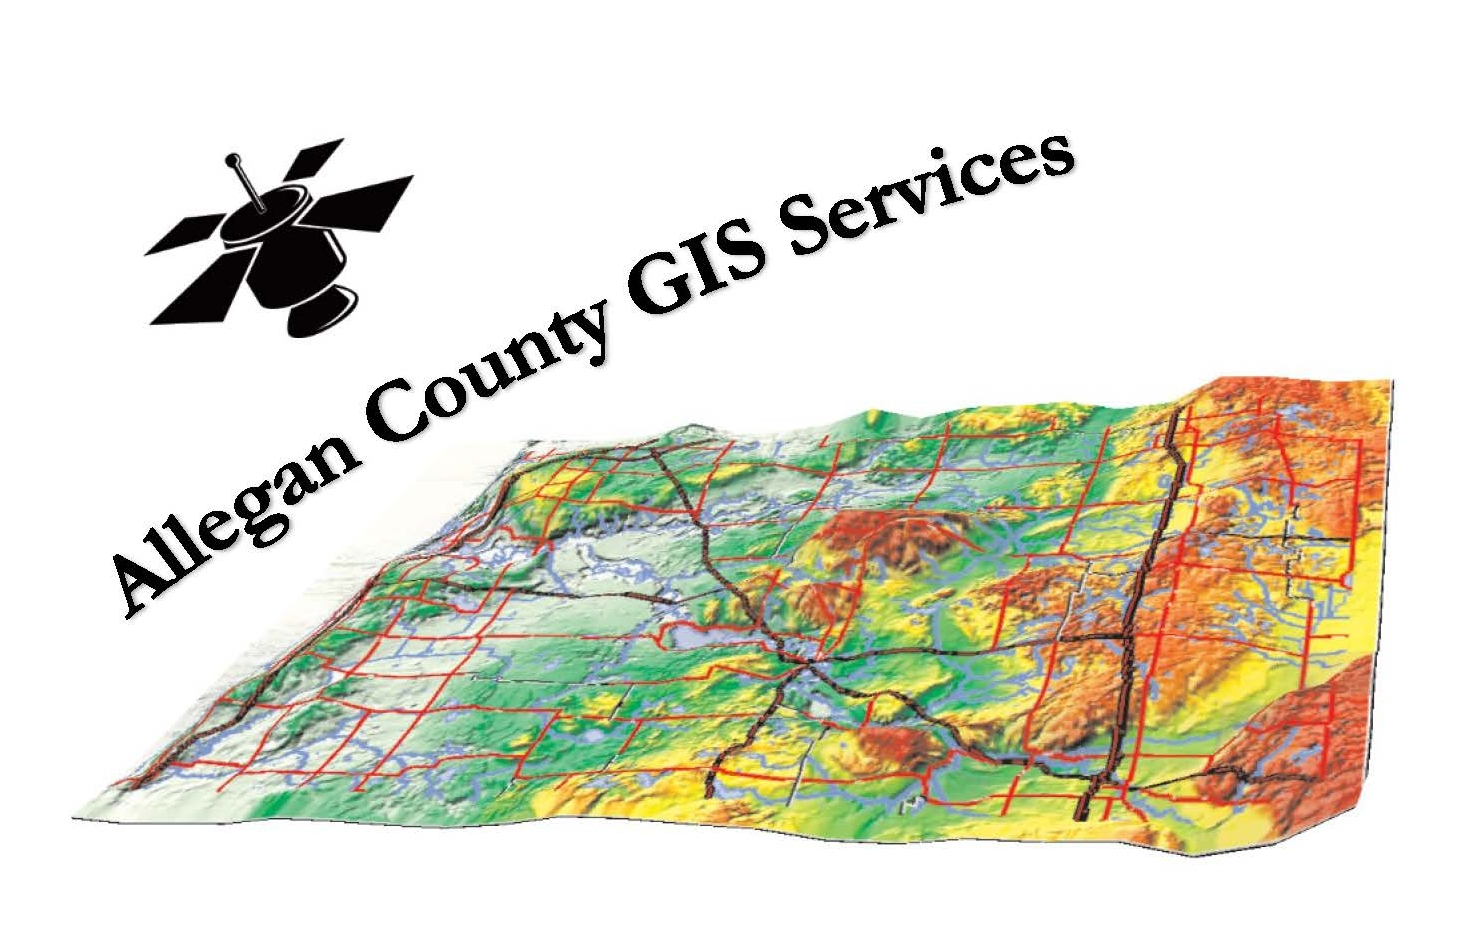
\includegraphics[scale=.45]{GIS_Logo_better.jpg}
\end{center}
\end{figure}
\Huge \bfseries \titlename \\ % Title text
\HRule \\[.4cm] % Horizontal Line added
\author{\Large Allegan County GIS \\\Large www.allegancounty.org/gis} % defines author
}  % inputs common title
\setcounter{tocdepth}{5}  % subparagraph and down
\begin{document}% document begins

\ifstandalone
\maketitle % creates title page
\clearpage
\tableofcontents % creates TOC
\clearpage
\fi

\subsection{Forfeiture Data Collection}

\subsubsection{Problem and Analysis}

\paragraph{Background}
Treasurer department has an annual responsibility to properly document the tax forfeiture process.  The LIS Department built an application in MS Access and MapInfo that consumed a daily export from BSA and was deployed to the field on a laptop.  A digital camera was used for site photos and later imported into the laptop.

\paragraph{Statement of Problem}
Current Tax Forfeiture workflow is built on MapInfo software which has been replaced by ESRI software.  The Forfeiture data collection application must be recreated in the ESRI framework.

\paragraph{Analysis}
Tax Forfeiture Application will facilitate:

\begin{itemize} %1

\item Mobile data collection on handheld device via Collector for ArcGIS configured with Allegan County GIS Portal  (\textbf{device app})

\begin{itemize} %2

\item Device app will:

\begin{itemize} %3

\item Synchronize with data in the office (online)
\item Navigate to forfeiture sites (offline)
\item Collect data and photos of forfeiture sites (offline)
\item Synchronize the collected data with data in the office (online)
\end{itemize} %3

\end{itemize} %2

\item Daily form production and printing for each site visited with required data and images.

\end{itemize} %1

\clearpage
\subsubsection{Design}
\paragraph{Overview}This Application utilizes Treasurer Department data to document the forfeiture process.  An enterprise GIS deployment enables offline data collection by up to two users.
\begin{figure}[h!]
\centering
    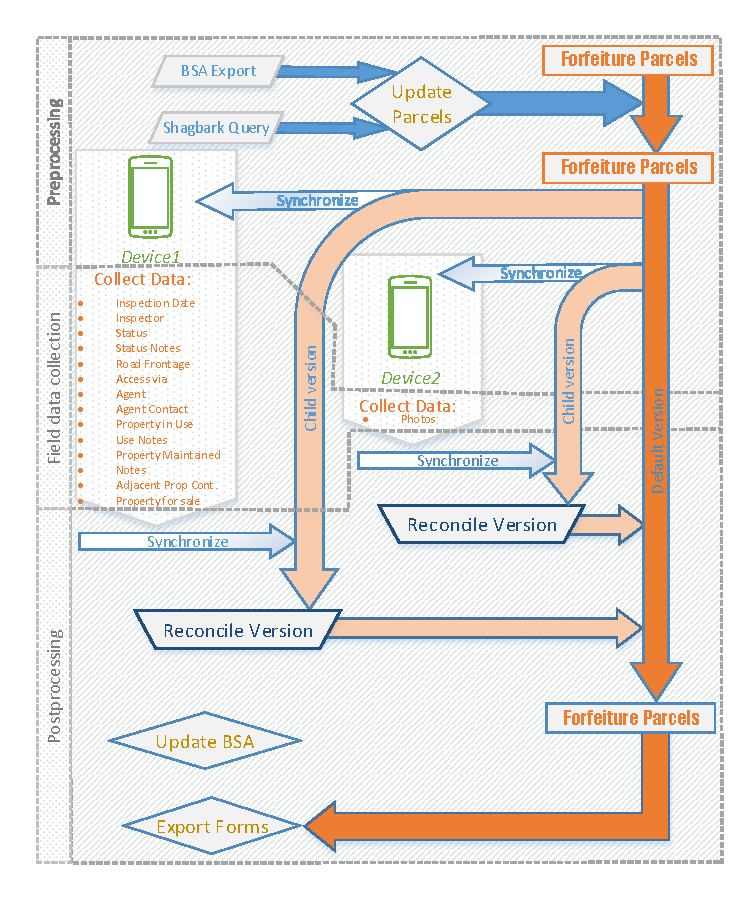
\includegraphics[width=.95\textwidth]{ProjectDesign}
    %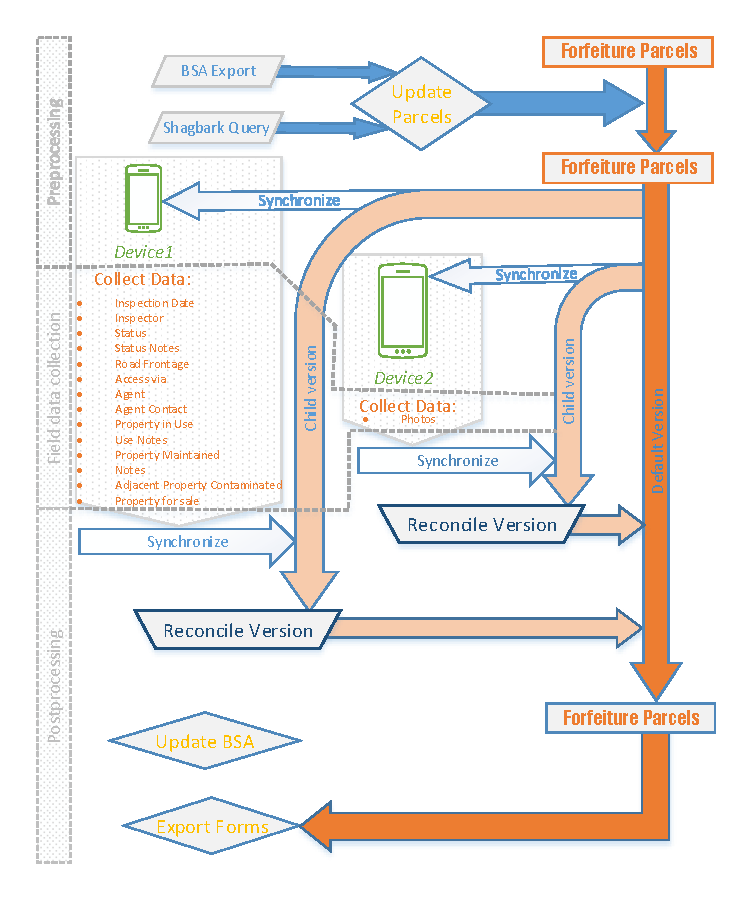
\includegraphics{DesignFlowChart}
\caption{Project Design}
\end{figure}
\subparagraph*{}There are three stages to daily workflow: Preprocessing, Field Collection, and Postprocessing.  Forfeiture Parcels, is a map feature class that is processed in the office via the network and remotely via the internet.
\clearpage
\subparagraph{Workflow Summary}
\begin{description}
\item [Preprocessing] The data is updated to match the Treasures data in BSAforfeiture.net and check for intersections with known contamination sites.  Data is then synchronized to two android mobile devices.
\item [Field data collection] The two mobile devices are used to collect info required, one for all the attributes, the other for photos.
\item[Postprocessing] The mobile devices are syncronized back to the network data and a form is exported for each site visited that day.
\end{description}

\medskip \paragraph{Technologies Used}
\subparagraph{BSA Data}Details of parcels in the forfeiture process are managed in BSA Delinquent Tax.net.  The Treasurer office does a BSA export of the parcels in need of a site visit in the preprocessing.

\subparagraph{ArcGIS Desktop}Tools are designed to preprocess and postprocess forfeiture parcel data for fieldwork.  The user will execute a preprocess script tool that prepares the data for field deployment.  After fieldwork, a post process script tool syncronizes data from the fieldwork with the live data on the Allegan County network. 

\subparagraph{ArcGIS Collector}A free mobile application developed and tested on Android is deployed to the field for data collection.  The application is configured to work offline(without an internet or cellular connection) by syncronizing before and after fieldwork.

\subparagraph{ArcGIS Portal Webmaps and Apps}Live data from a publishing enterprise geodatabase(ACPub), running on SQL Server database server (acintsql01) is provided through a feature service (REST service)  named TaxReversionParcels.  A webmap called the Forfeiture Field Map consumes the TaxReversionParcels feature service, exposing the data to editing.  The Forfeiture Field Map is configured to work in the ArcGIS Collector App.  The app downloads the webmap, allowing the user to collect the necessary information on each forfeiture parcel in the field disconnected, and then to upload the changes when reconnected. 

\paragraph{Forfeiture Mobile Data Collection App in Action}

Three parts of the daily routine:
\begin{enumerate}
\item \Large Preprocessing \normalsize(in the office):

\begin{itemize}
\item Export current forfeiture list from BSA
\item Update webmap layers with results from BSA export
\item Update webmap layers with results of an intersect routine with contaminated sites  
\item Synchronize from webmap layers to field collection devices \textbf{(device app)}
\end{itemize}

\item \Large Field data collection \normalsize with device app:

\begin{itemize}
\item Navigation to forfeiture sites is aided by users location shown in map
\item A Checklist of data points about the site
\item Attach photos to the site
\item Save results for synchronization in post-processing
\end{itemize}

\item \Large Post-processing \normalsize (in the office)

\begin{itemize}
\item Synchronize data and images collected in device app to webmap layers

\end{itemize}
\end{enumerate}

\clearpage
\paragraph{Data Details}
\subparagraph*{Location}

\begin{wrapfigure}{r}{0.5\textwidth}
\centering
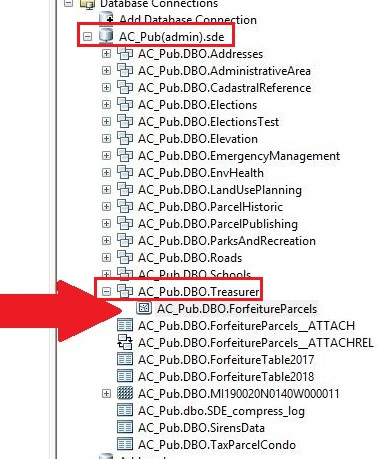
\includegraphics[width=.45\textwidth]{LiveDataLocation}
\caption{Live Data Location}
\vspace{.25in}
\HRule \\[.4cm] % Horizontal Line added
\vspace{.25in}
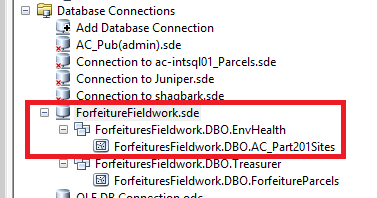
\includegraphics[width=.3\textwidth]{contaminationFeatureClass.png}
\caption{Contamination Feature Class}
\end{wrapfigure}
The data is located in ACPUB.  ACPUB is a geodatabase on ACINTSQL01.
\vspace{.5in}

Forfeiture Parcels Data
\vspace{3.5in}

Contamination Data
\clearpage
\subparagraph{ForfeitureParcels Feature Class}
\begin{table}
\centering
\begin{tabular}{|l|l|c|r|}
\hline
\multicolumn{4}{|c|}{{\LARGE Attribute List}} \\
\hline
Field Name&Field Alias&Entry Type&Note\\ \hline
PropertyNumber&Property Number&Prefilled&NA\\
Need2Print&Print Today&Dropdown&Yes or No\\
InspectionDate&InspectionDate&{\scriptsize Autofill or Dropdown}&NA\\
Inspector&Inspector&Dropdown&NA\\
Address&Address&Prefilled&NA\\
Status&Status&Dropdown&NA\\
StatusNotes&Status Notes&Open Entry&120Char\\
Roadfrontage&Road Frontage&Dropdown&Yes or No\\
AccessVia&Access via&Open Entry&30Char\\
Agent&Agent&Open Entry&30Char\\
AgentContact&Agent Contact&Open Entry&30Char\\
UseNotes&Use Notes&Open Entry&120Char\\
PropMaintNotes&{\footnotesize Property Maintained Notes}&Open Entry&120Char\\
PropertyForSale&Property for sale&Dropdown&Yes or No\\
Posted&Posted&Prefilled&NA\\
InList&In List&Prefilled&in Preproc\\
PostedInList&PostedInList&Prefilled&in Preproc\\
Acres&Acres&Prefilled&NA\\
Class&Class&Prefilled&NA\\
PropertyInUse&Property In Use&Dropdown&Yes or No\\
PropertyMaintained&Property Maintained&Dropdown&Yes or No\\
PropertyContaminated&Property Contaminated&Prefilled&in Preproc\\
Notes&Notes&Open Entry&120Char\\
{\footnotesize AdjacentPropertyContaminated}&{\footnotesize Adjacent Property Contaminated}&Prefilled&in Preproc\\
{\footnotesize PropertyContaminatedNotes}&{\footnotesize PropertyContaminatedNotes}&Prefilled&in Preproc\\
{\footnotesize AdjPropertyContaminatedNotes}&{\footnotesize AdjPropertyContaminatedNotes}&Prefilled&in Preproc\\
PictureComments&Picture1Comments&Open Entry&50Char\\
PostedDate&PostedDate&Dropdown&Date\\
\hline
\end{tabular}
\caption{Dataset Details}
\end{table}

\clearpage
\paragraph{Webmap Details}The Forfeiture Field Map can be accessed on PC through the Allegan County GIS Portal.  The map is made up of a basemap and a feature layer.
\begin{figure}[h!]
\centering
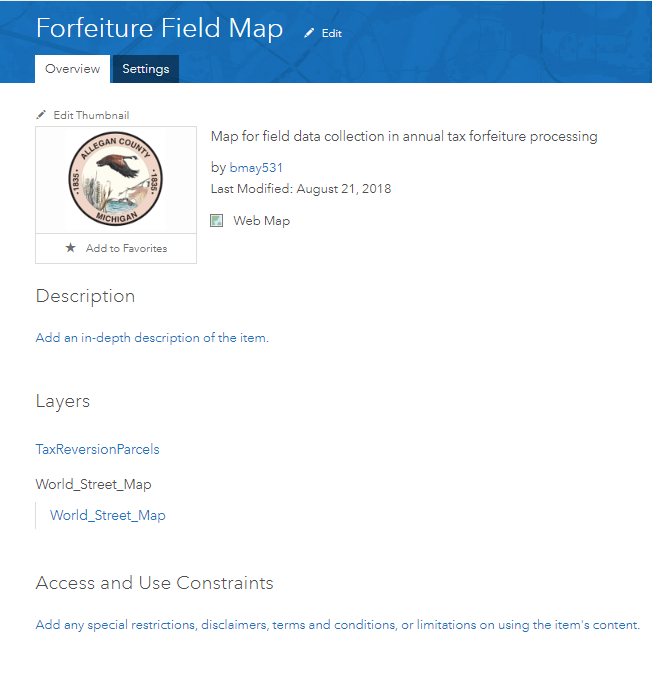
\includegraphics[width=.6\textwidth]{webMapDetails}
\caption{Web Map Details}
\end{figure}

\subparagraph{Feature Layer Details}The webmap consists of a basemap and a feature layer, TaxReversionParcels.  TaxReversionParcels has been configured for offline use.
\begin{figure}[h!]
\centering
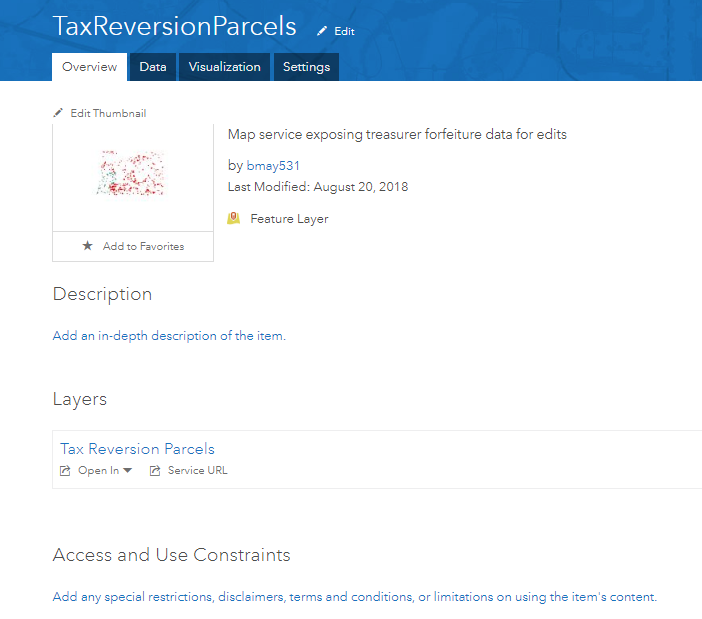
\includegraphics[width=.6\textwidth]{layerDetails}
\caption{Layer Details}
\end{figure}
\clearpage



%images of publishing the service and explanation of settings required for offline use




\subparagraph{Basemap Details}A tiled basemap service is used.  The infoserv user credentials are used for sharing.  The url for the shared service is:
\begin{verbatim}
https://tiledbasemaps.arcgis.com/arcgis/rest/
   services/World_Street_Map/MapServer
\end{verbatim}
\begin{figure}[h!]
\centering
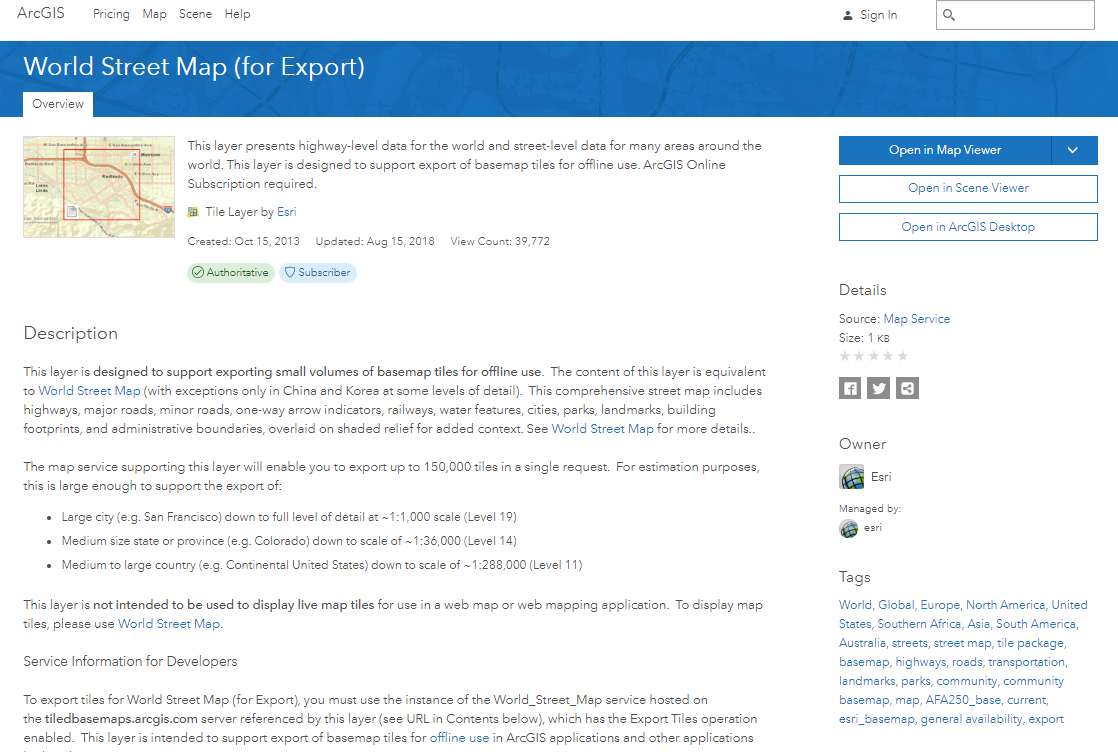
\includegraphics[width=.7\textwidth]{BasemapSourceDescription}
\caption{Basemap Source Description}
\end{figure}
\clearpage


%Unplaced images
\subparagraph{unplaced images}
\begin{figure}[h!]
\centering
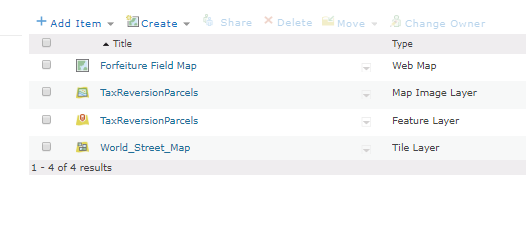
\includegraphics[width=.7\textwidth]{PortalContents}
\caption{Portal Contents}
\end{figure}
%\subparagraph{Feature layer configuration}
%\begin{figure}[h!]
%\centering
%\includegraphics[width=.7\textwidth]{featureLayerConfig}
%\caption{Feature Layer Configuration}
%\end{figure}

\begin{figure}[h!]
\centering
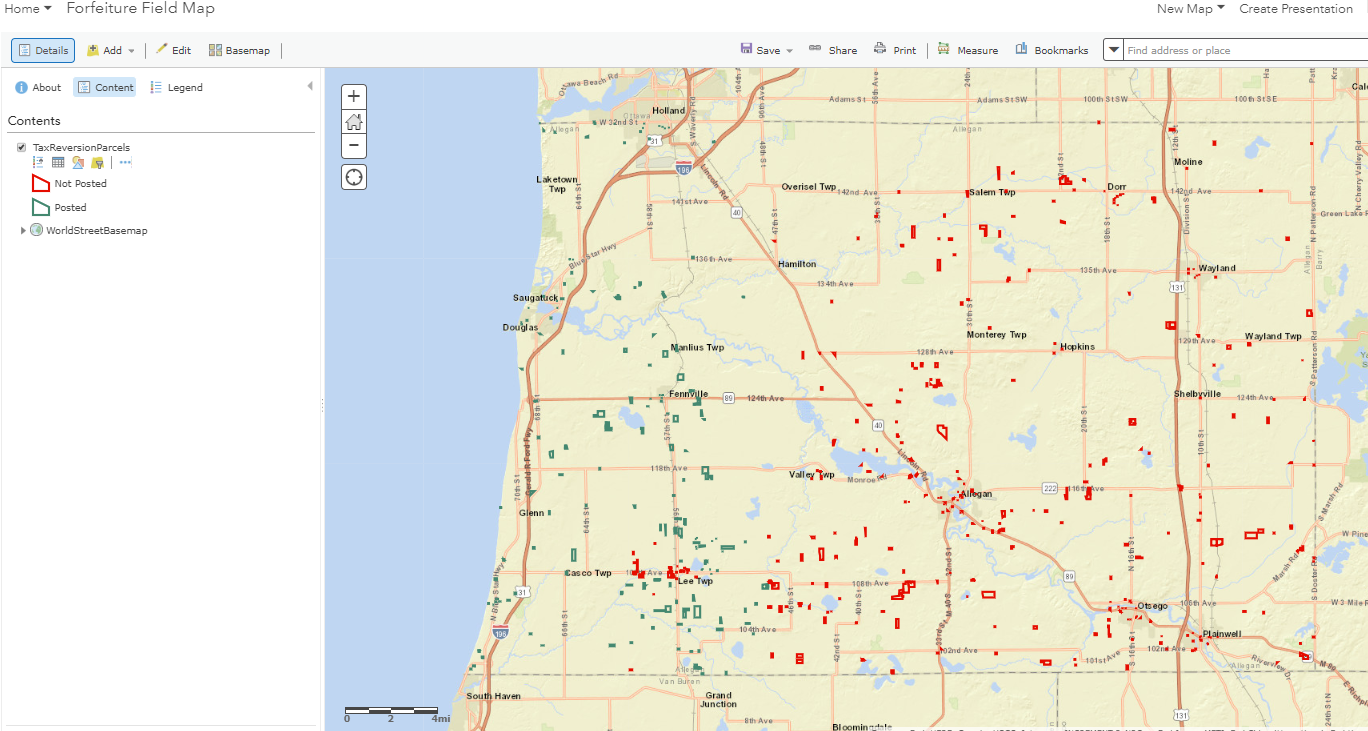
\includegraphics[width=.5\textwidth]{FieldMapOnPC}
\caption{Field Map on PC}
\end{figure}

\clearpage
\subsubsection{Hard Copy Record}
screenshots:
arcmap map 
arcmap tools
portal screenshots
sql server mgt screen shots
phone screenshots

\paragraph{ArcGIS Server}

\paragraph{xx}


\clearpage
\subsubsection{User Manual}

\paragraph{Administrative Tasks}

\subparagraph{Annual Setup}

\subparagraph{Setup Users in ArcGIS}Users that will run Pre and Post processing scripts must be created and given priviliges on ACPub Treasurer Feature Data Set.

\subparagraph{Setup Users in Portal for ArcGIS}Users that will use the Collector for ArcGIS must have profiles added to and managed in the Allegan County GIS Portal site.

\subparagraph{Schema Change Procedure}

\subparagraph{Form Edits Procedure}

\clearpage
\paragraph{Collection Device Setup}

\paragraph{Collector Application Setup Details}

\subparagraph{Install Collector for ArcGIS}
\begin{itemize}
\item Available from the Google Play Store
\end{itemize}
\begin{figure}[h!]
\centering
    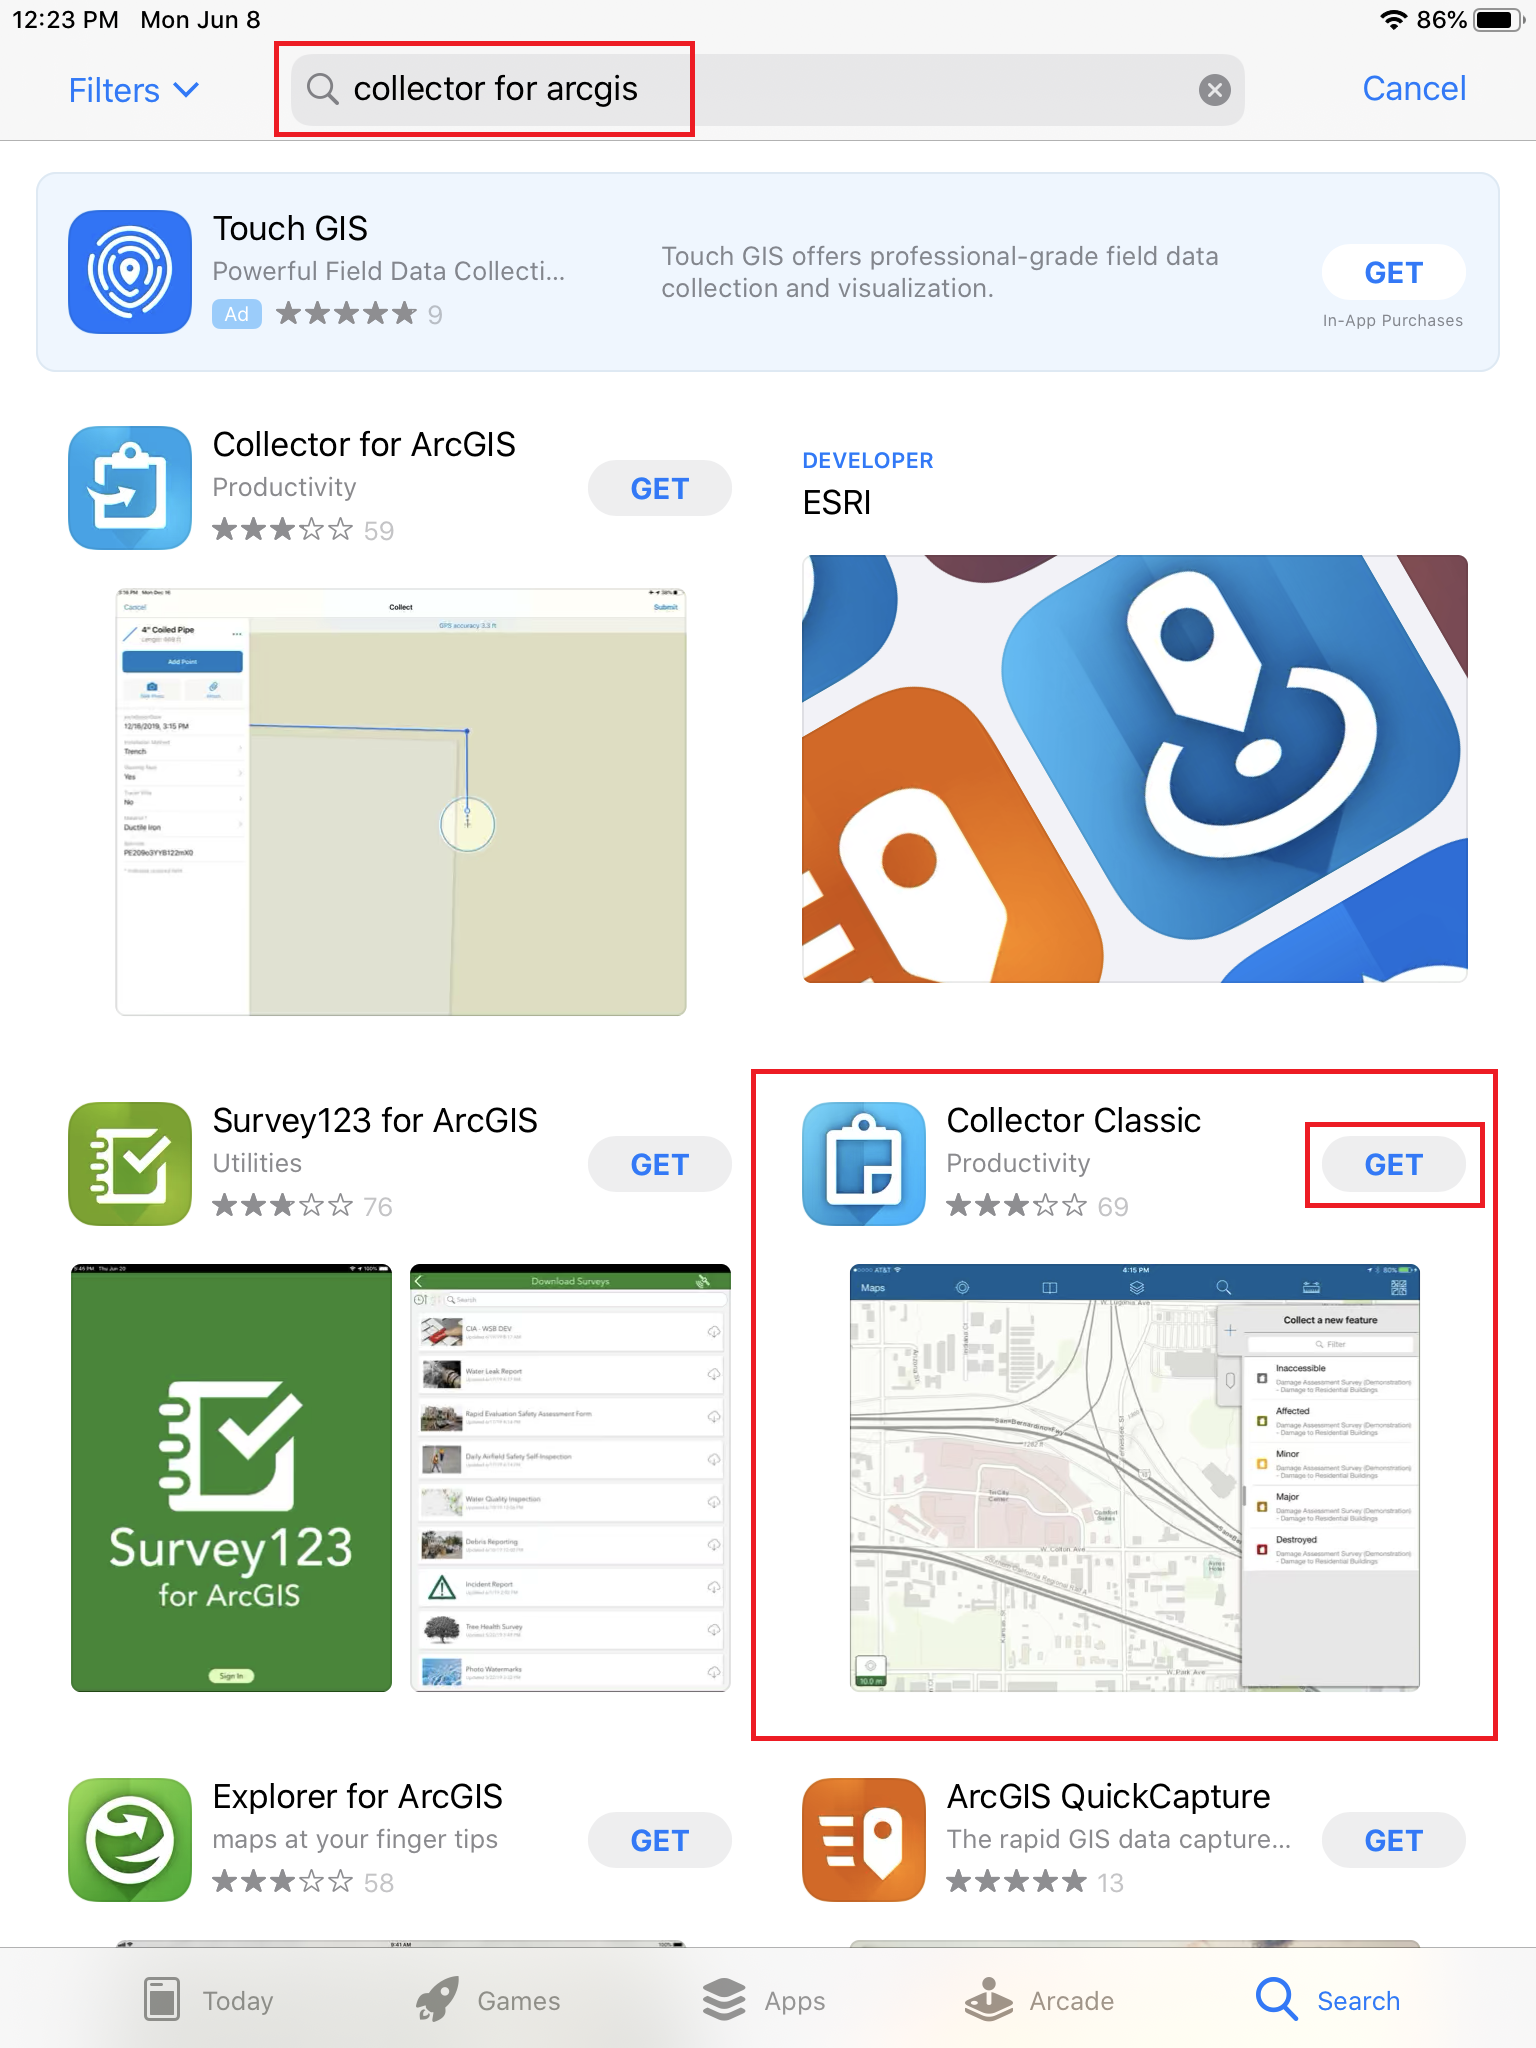
\includegraphics[width=.65\textwidth]{DownloadtheApp.png}
\caption{Download the App}
\end{figure}

\clearpage
\subparagraph{Configure Collector}

\subparagraph*{\\}
\begin{wrapfigure}{r}{0.5\textwidth}
\centering
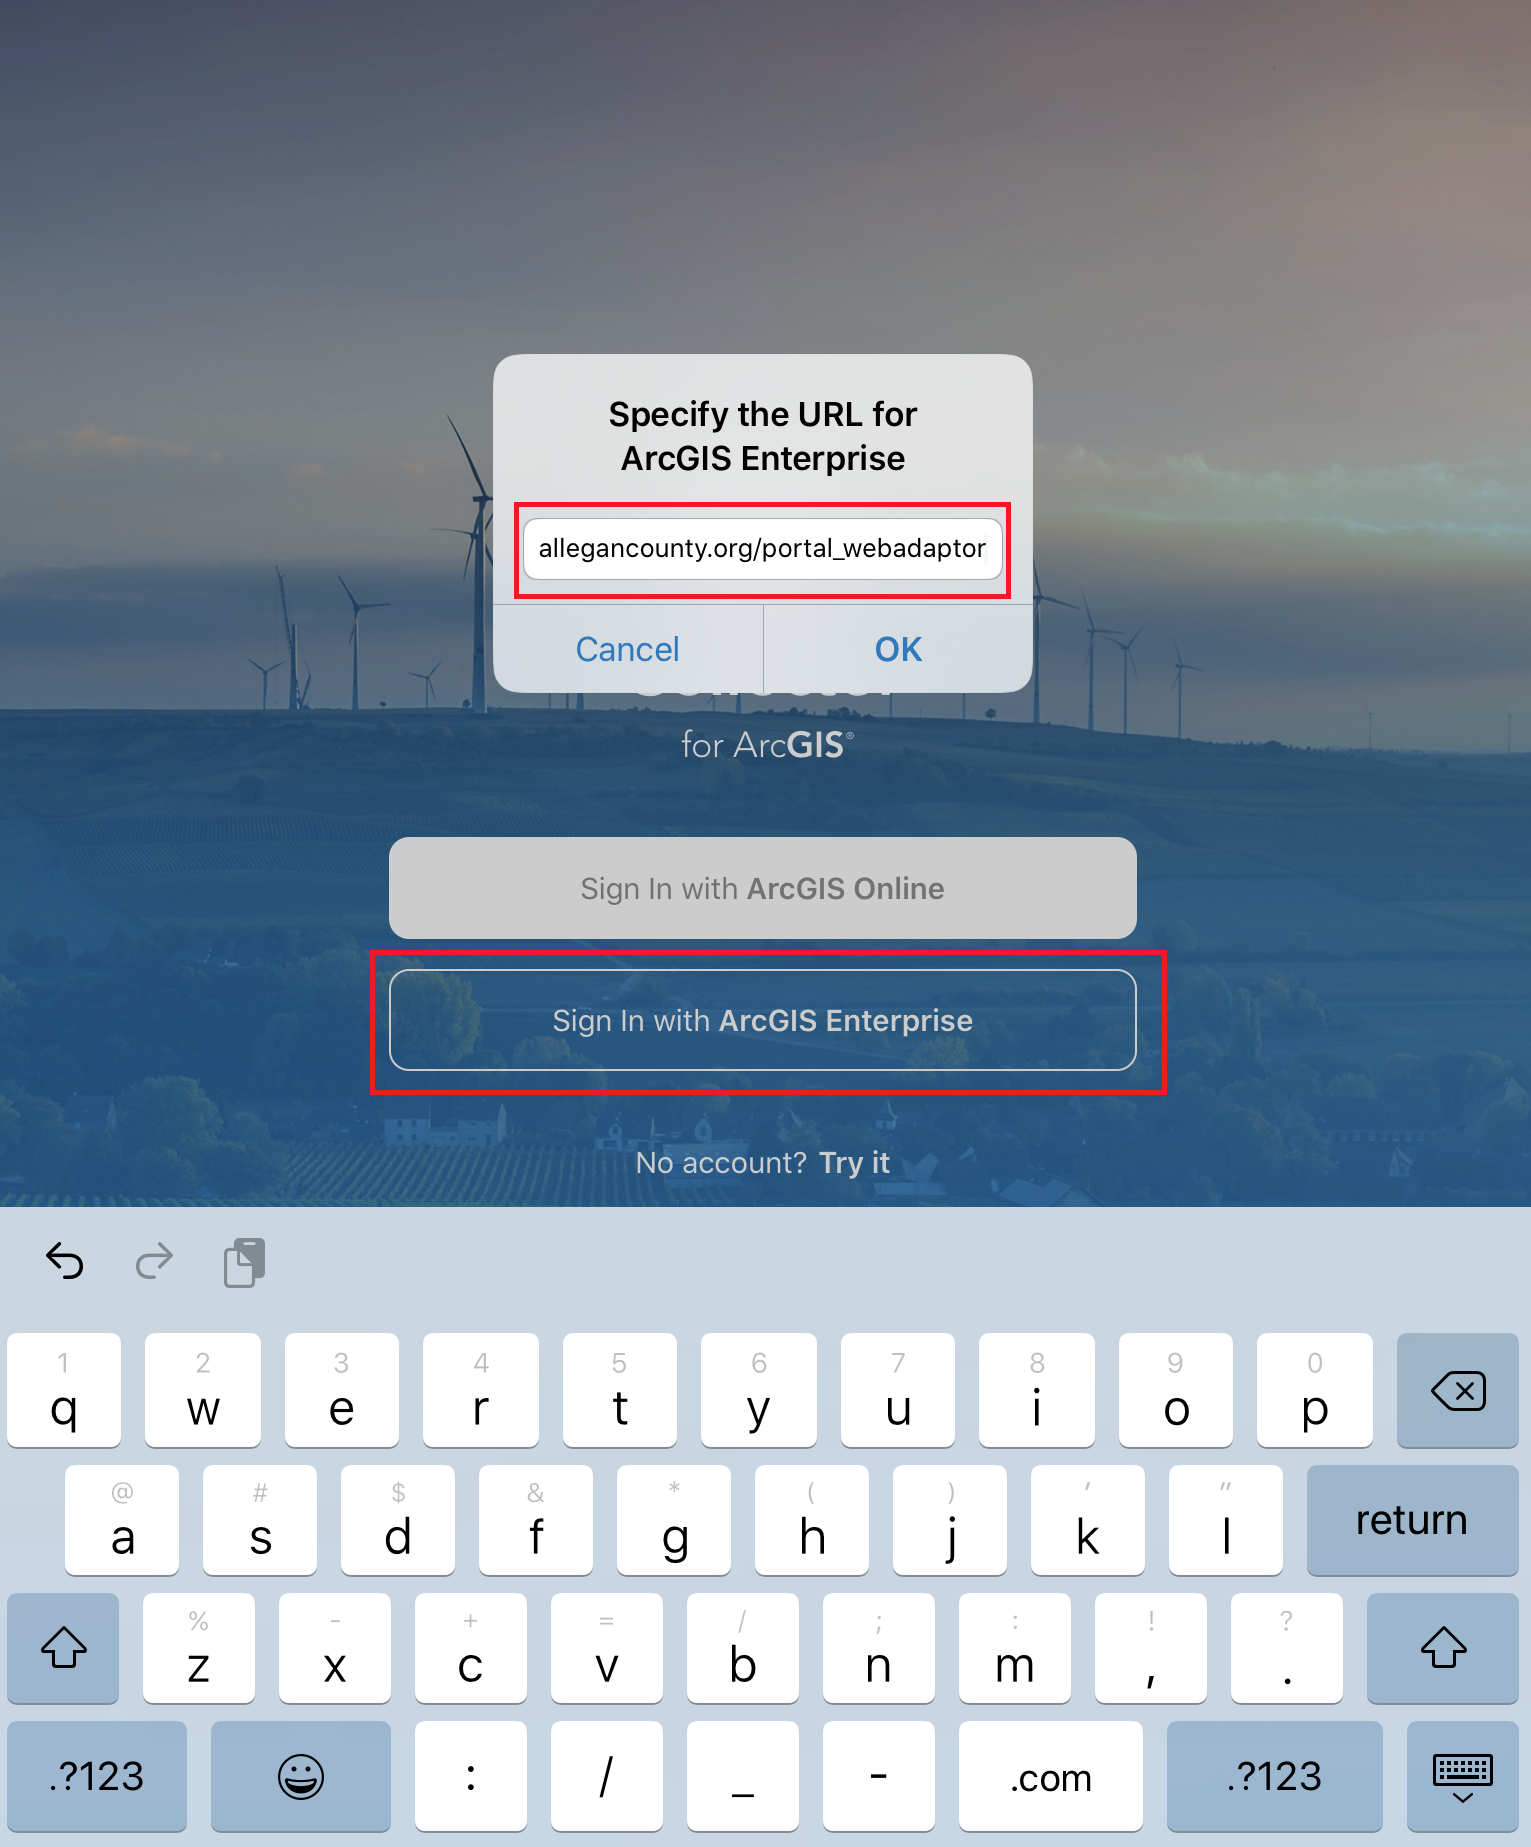
\includegraphics[width=.3\textwidth]{CollectorConnection}
\caption{Collector Connection}
\vspace{.25in}
\HRule \\[.4cm] % Horizontal Line added
\vspace{.25in}
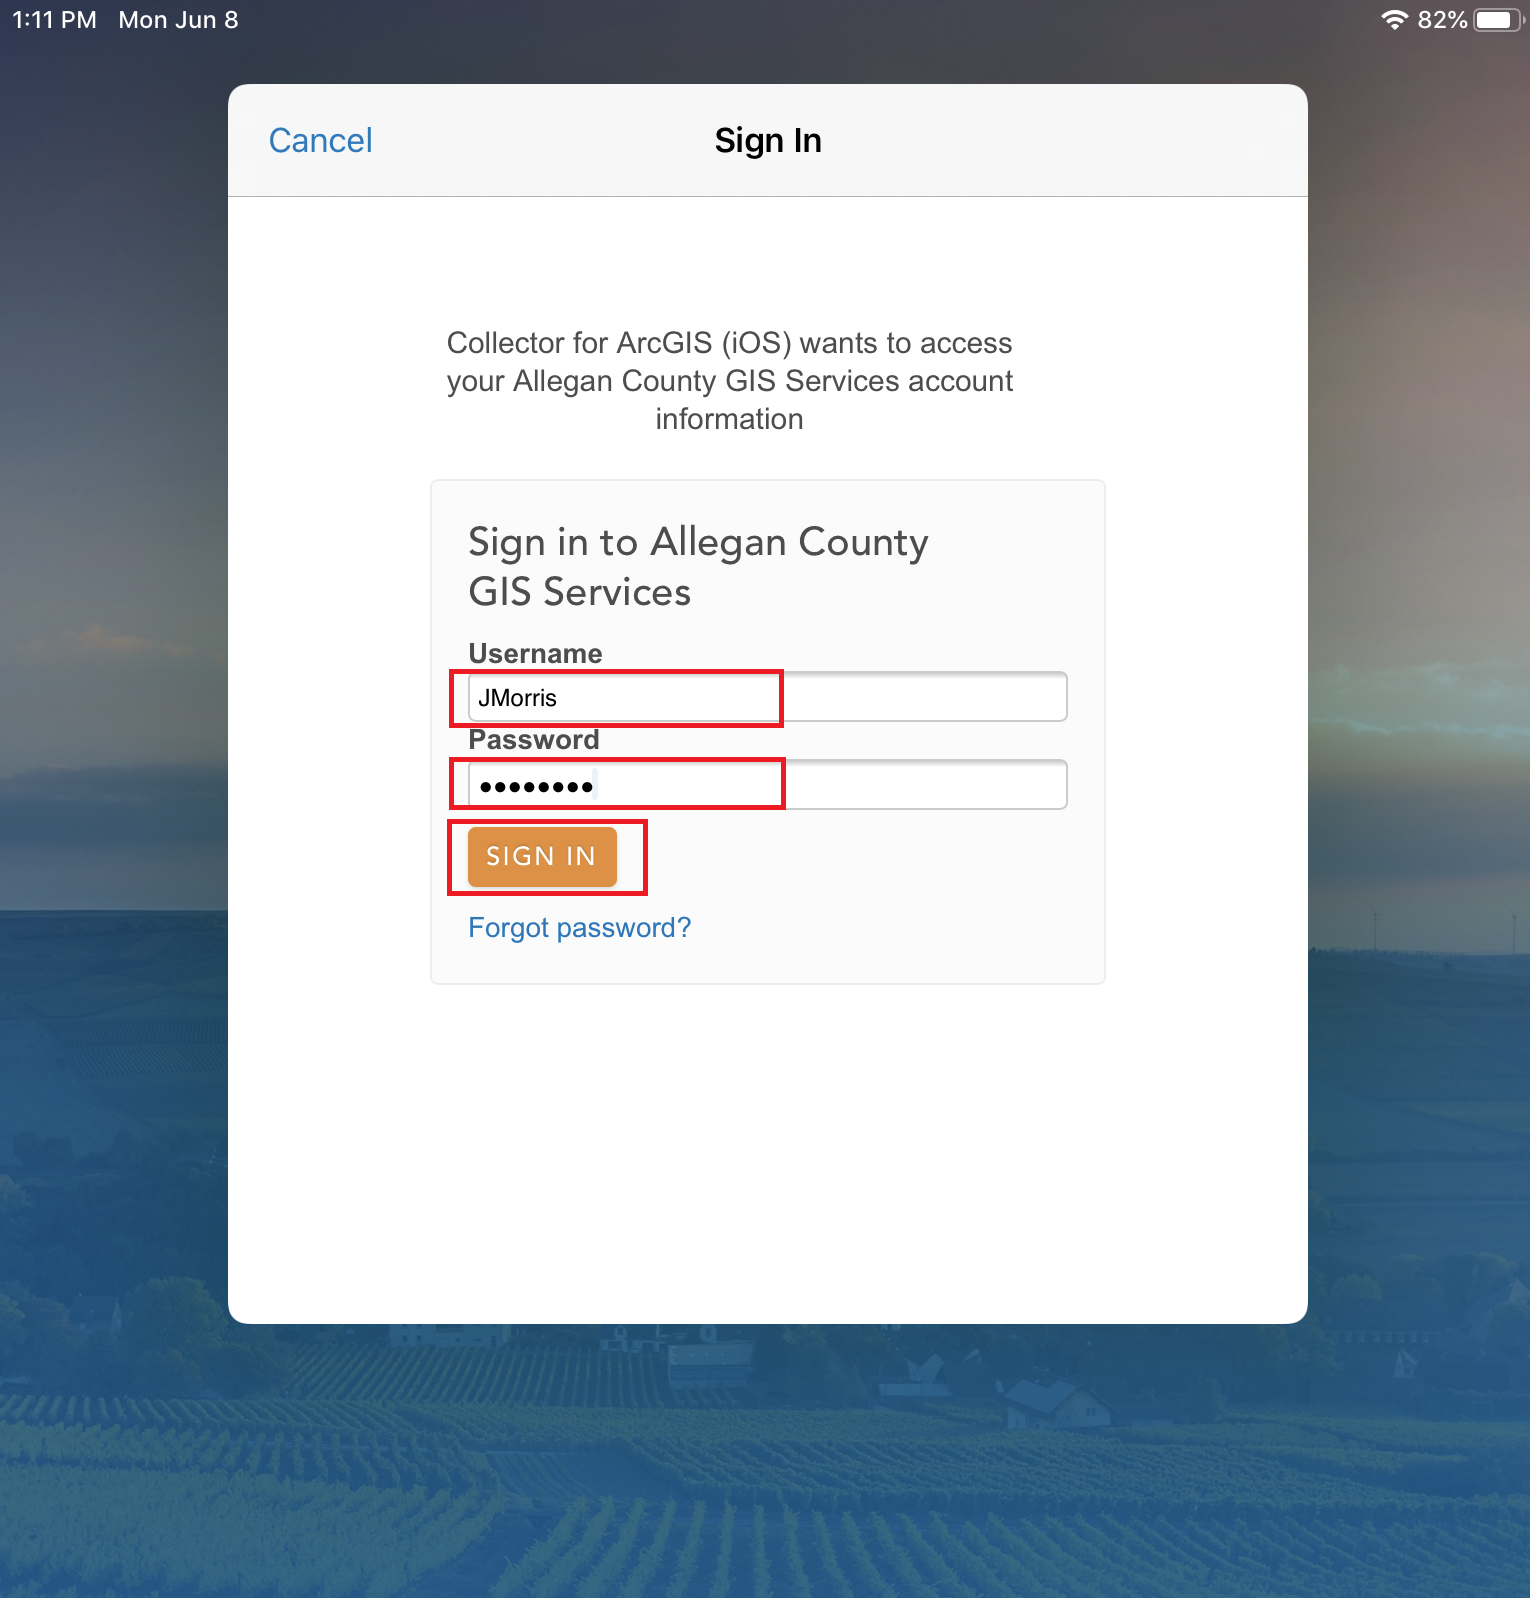
\includegraphics[width=.3\textwidth]{EnterCredentials.png}
\caption{Enter Credentials}
\end{wrapfigure}
for Organization Website, Type:
\vspace{.5in}

\begin{verbatim}
https://gis.allegancounty.org/
portal_webadaptor

\end{verbatim}
then:\\
Press \Large Continue
\vspace{3in}
Enter Credentials\\
then:\\
Press \Large SIGN IN
\clearpage
\subparagraph{Download the Forfeiture Field Map}
There are 3 different versions of the map.
\subparagraph*{\\}
\begin{wrapfigure}{r}{0.5\textwidth}
\centering
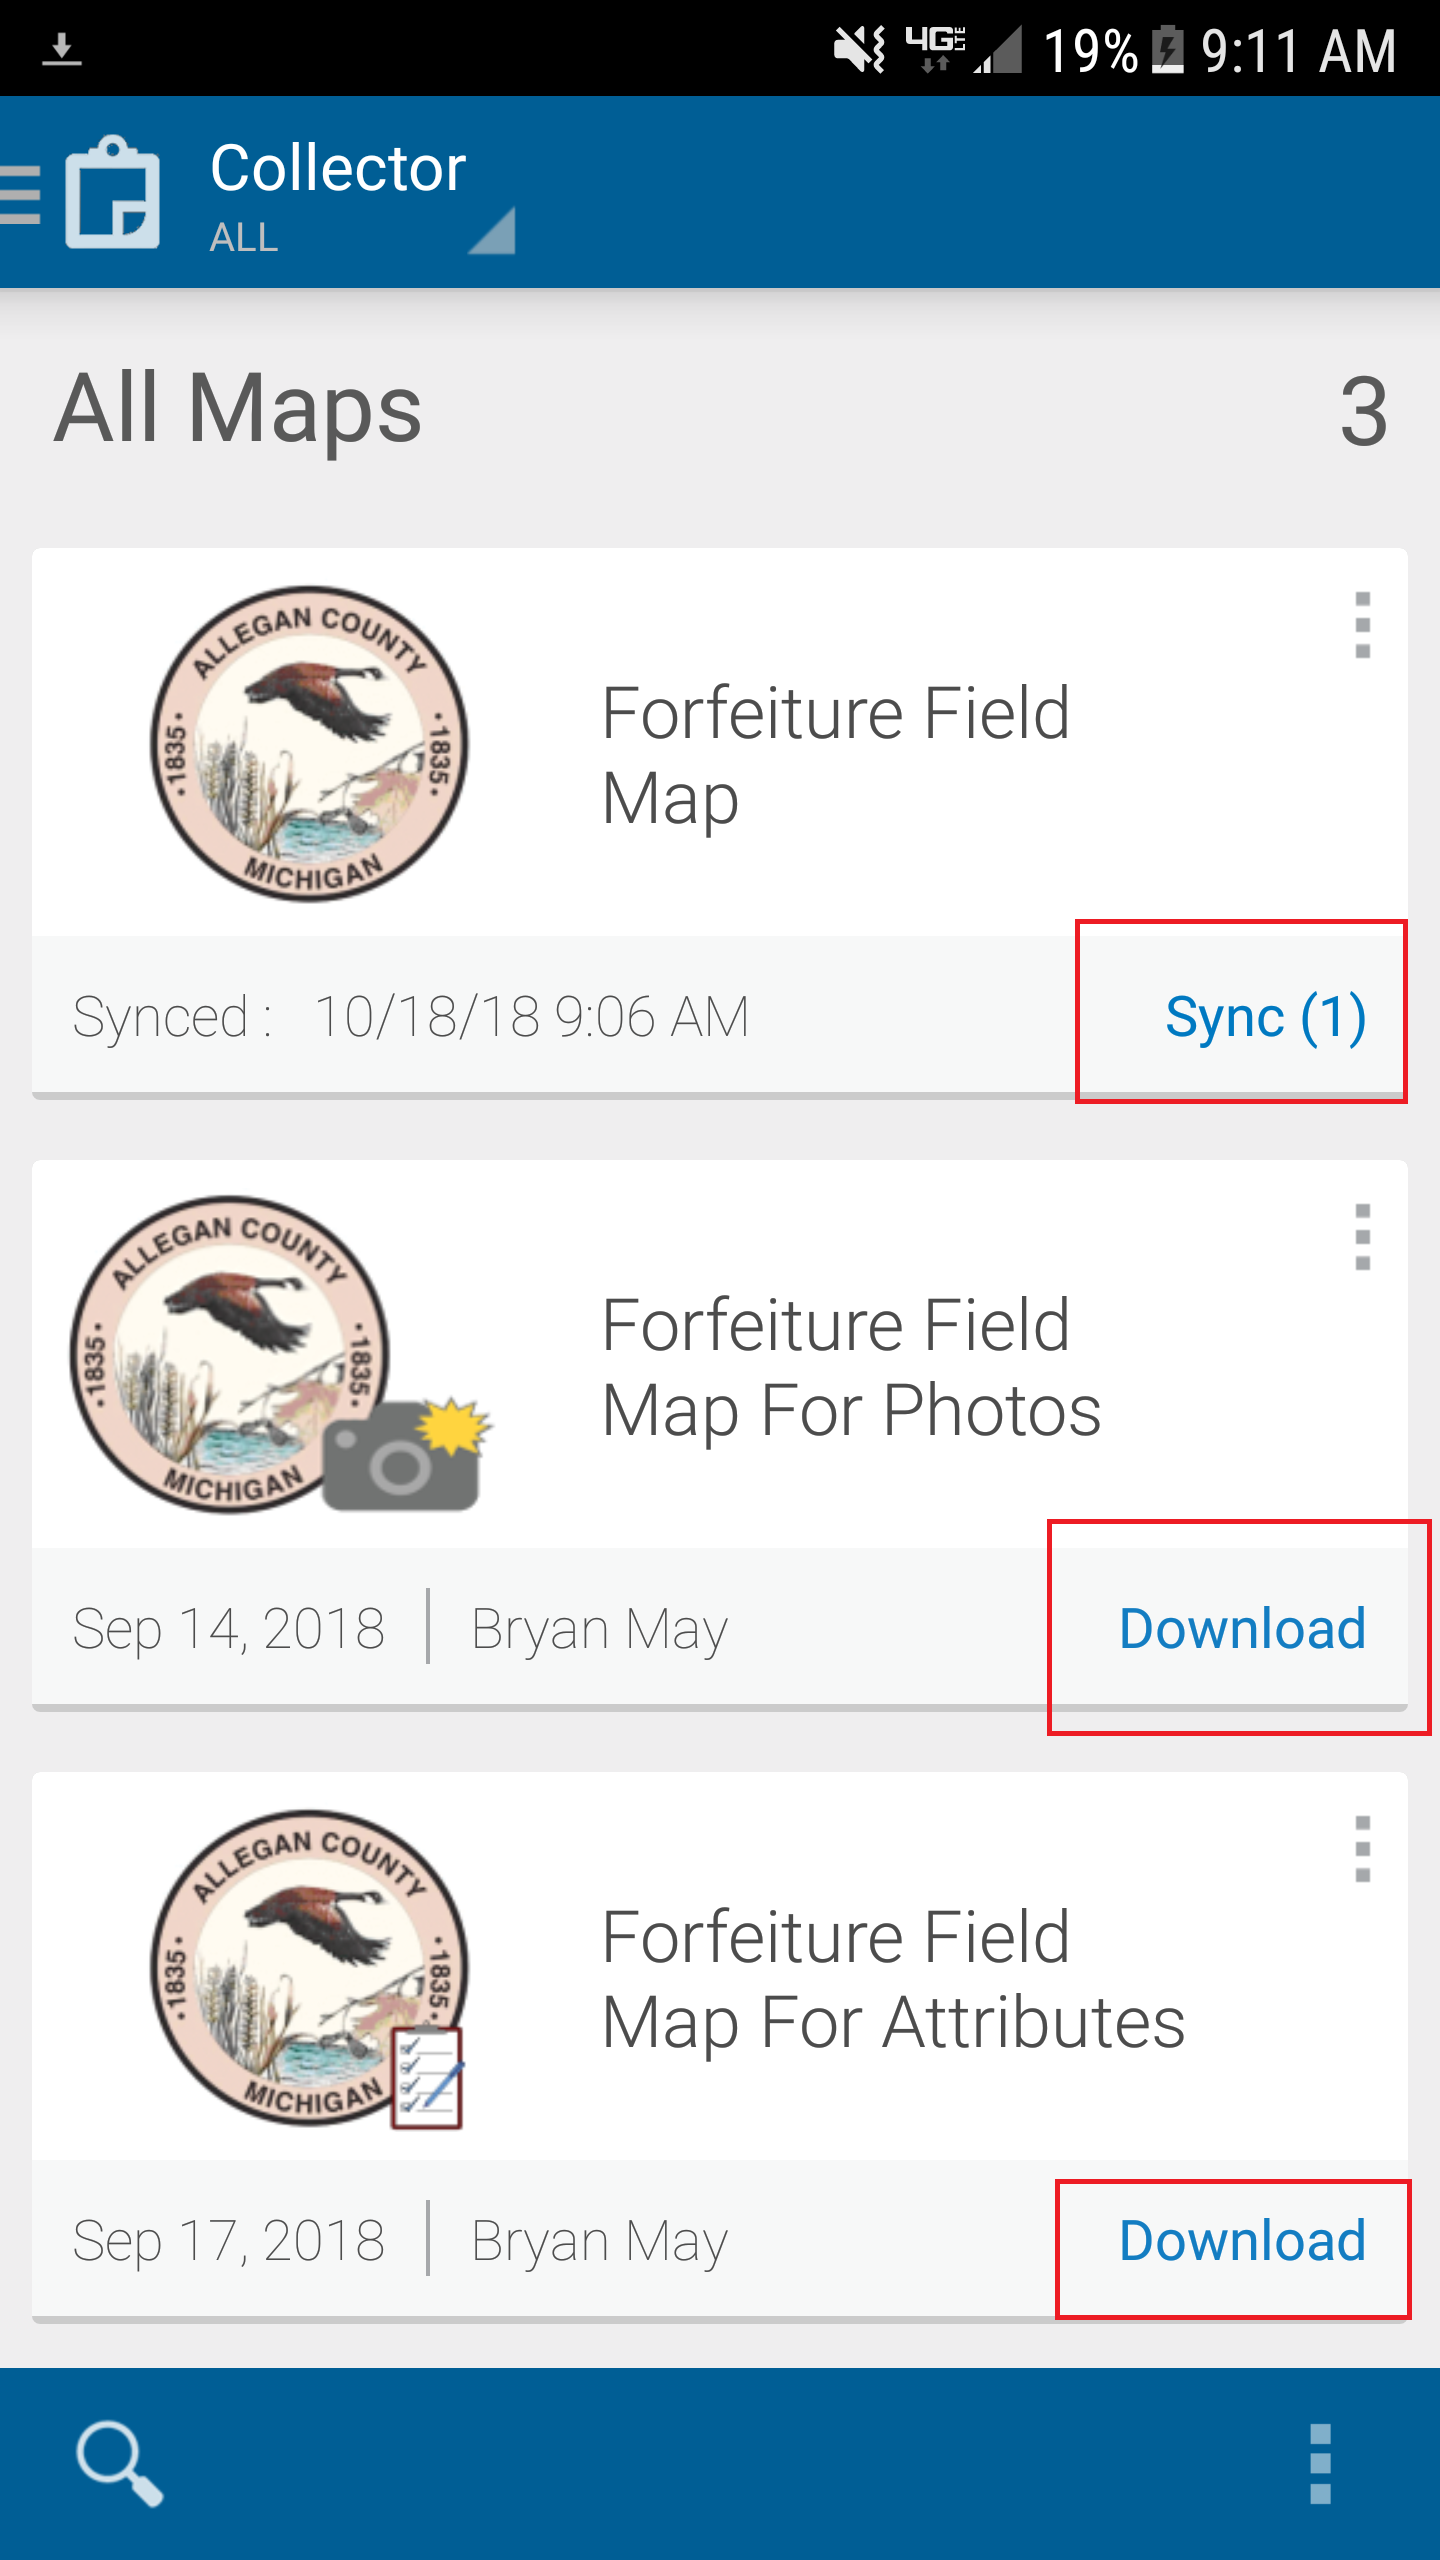
\includegraphics[width=.5\textwidth]{CollectorChooseMap.png}
\caption{Collector Maps Menu}
\end{wrapfigure}
\begin{itemize}
\item Forfeiture Field Map
\item Forfeiture Field Map For Photos
\item Forfeiture Field Map For Attributes
\end{itemize}
\clearpage
\subparagraph*{\\}
\begin{wrapfigure}{r}{0.5\textwidth}
\centering
%\vspace{.25in}
%\HRule \\[.4cm] % Horizontal Line added
%\vspace{.25in}
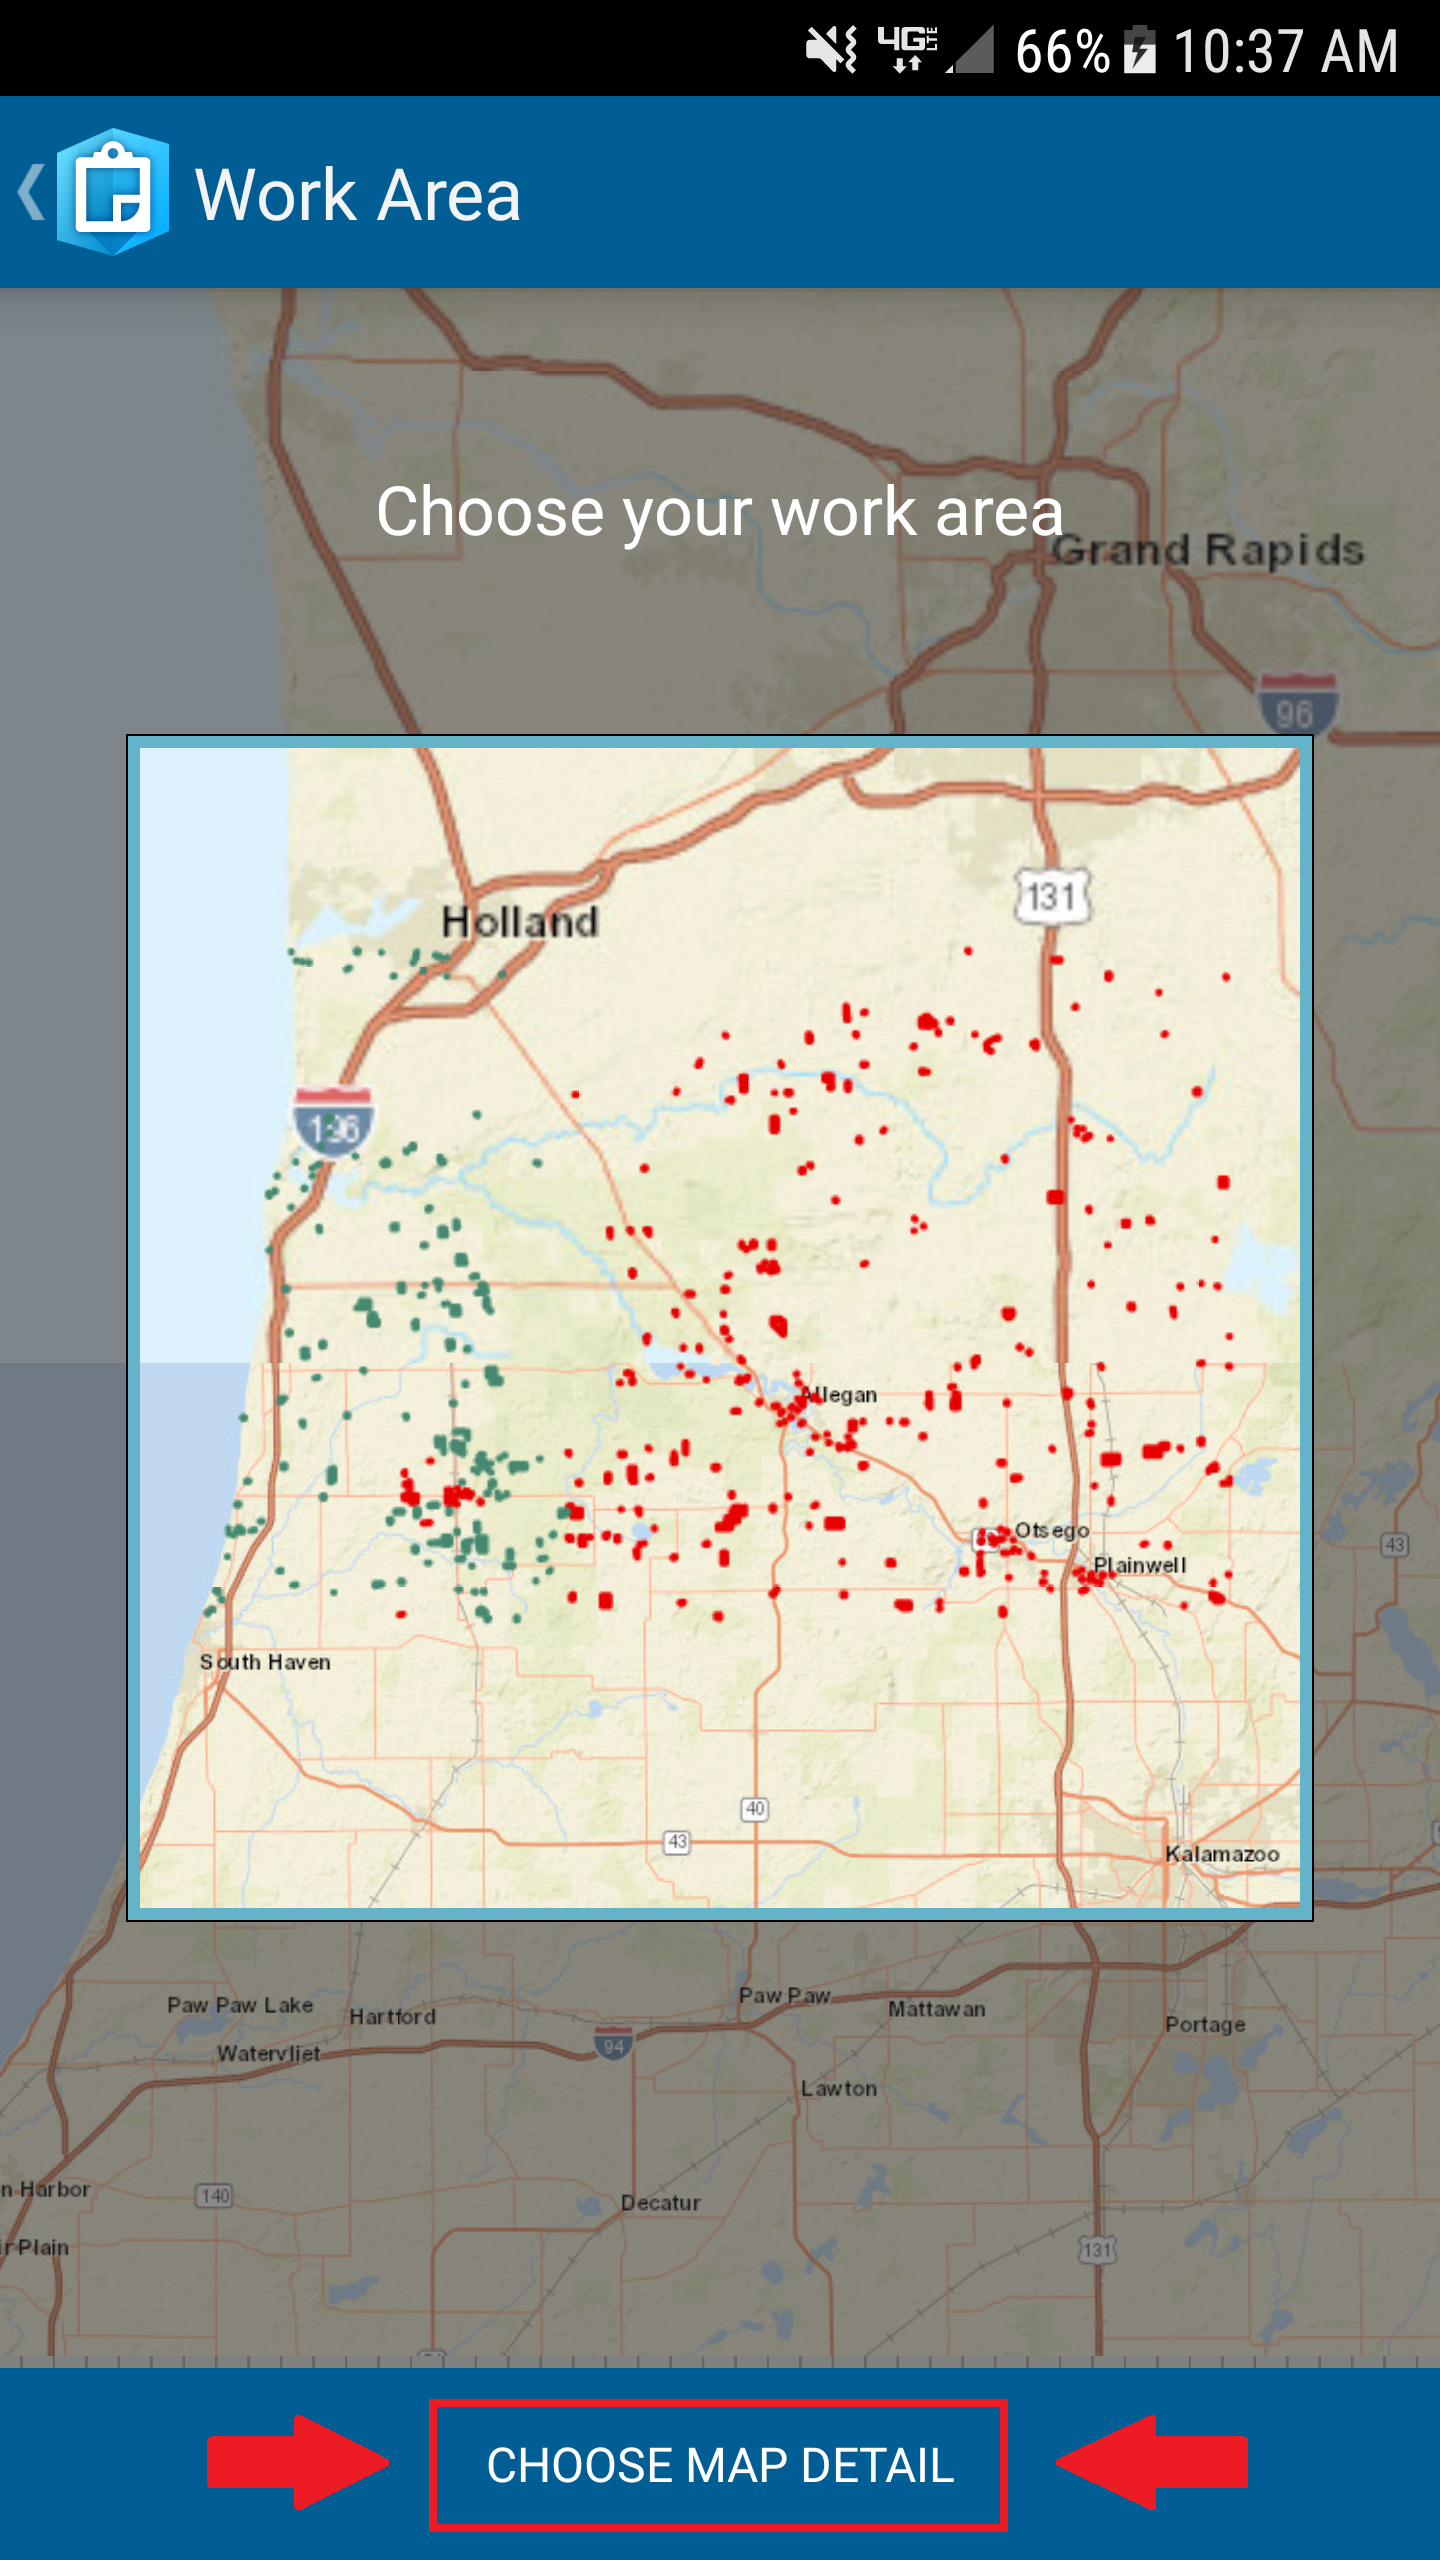
\includegraphics[width=.3\textwidth]{ChooseWorkAreaLarge.png}
\caption{Choose Work Area (large)}
\end{wrapfigure}
The Download option indicates it is not on the device but is available for offline use.
\vspace{.5in}

\noindent Press \Large Download\\
\vspace{3in}

\noindent Specify work area to download and press \Large map detail\\
\vspace{.5in}

\noindent \footnotesize Note that a larger area takes longer to download but the basemap only needs to be downloaded once.
\clearpage
\subparagraph{Choose Map Detail}

\subparagraph*{\\}
\begin{wrapfigure}{r}{0.5\textwidth}
\centering
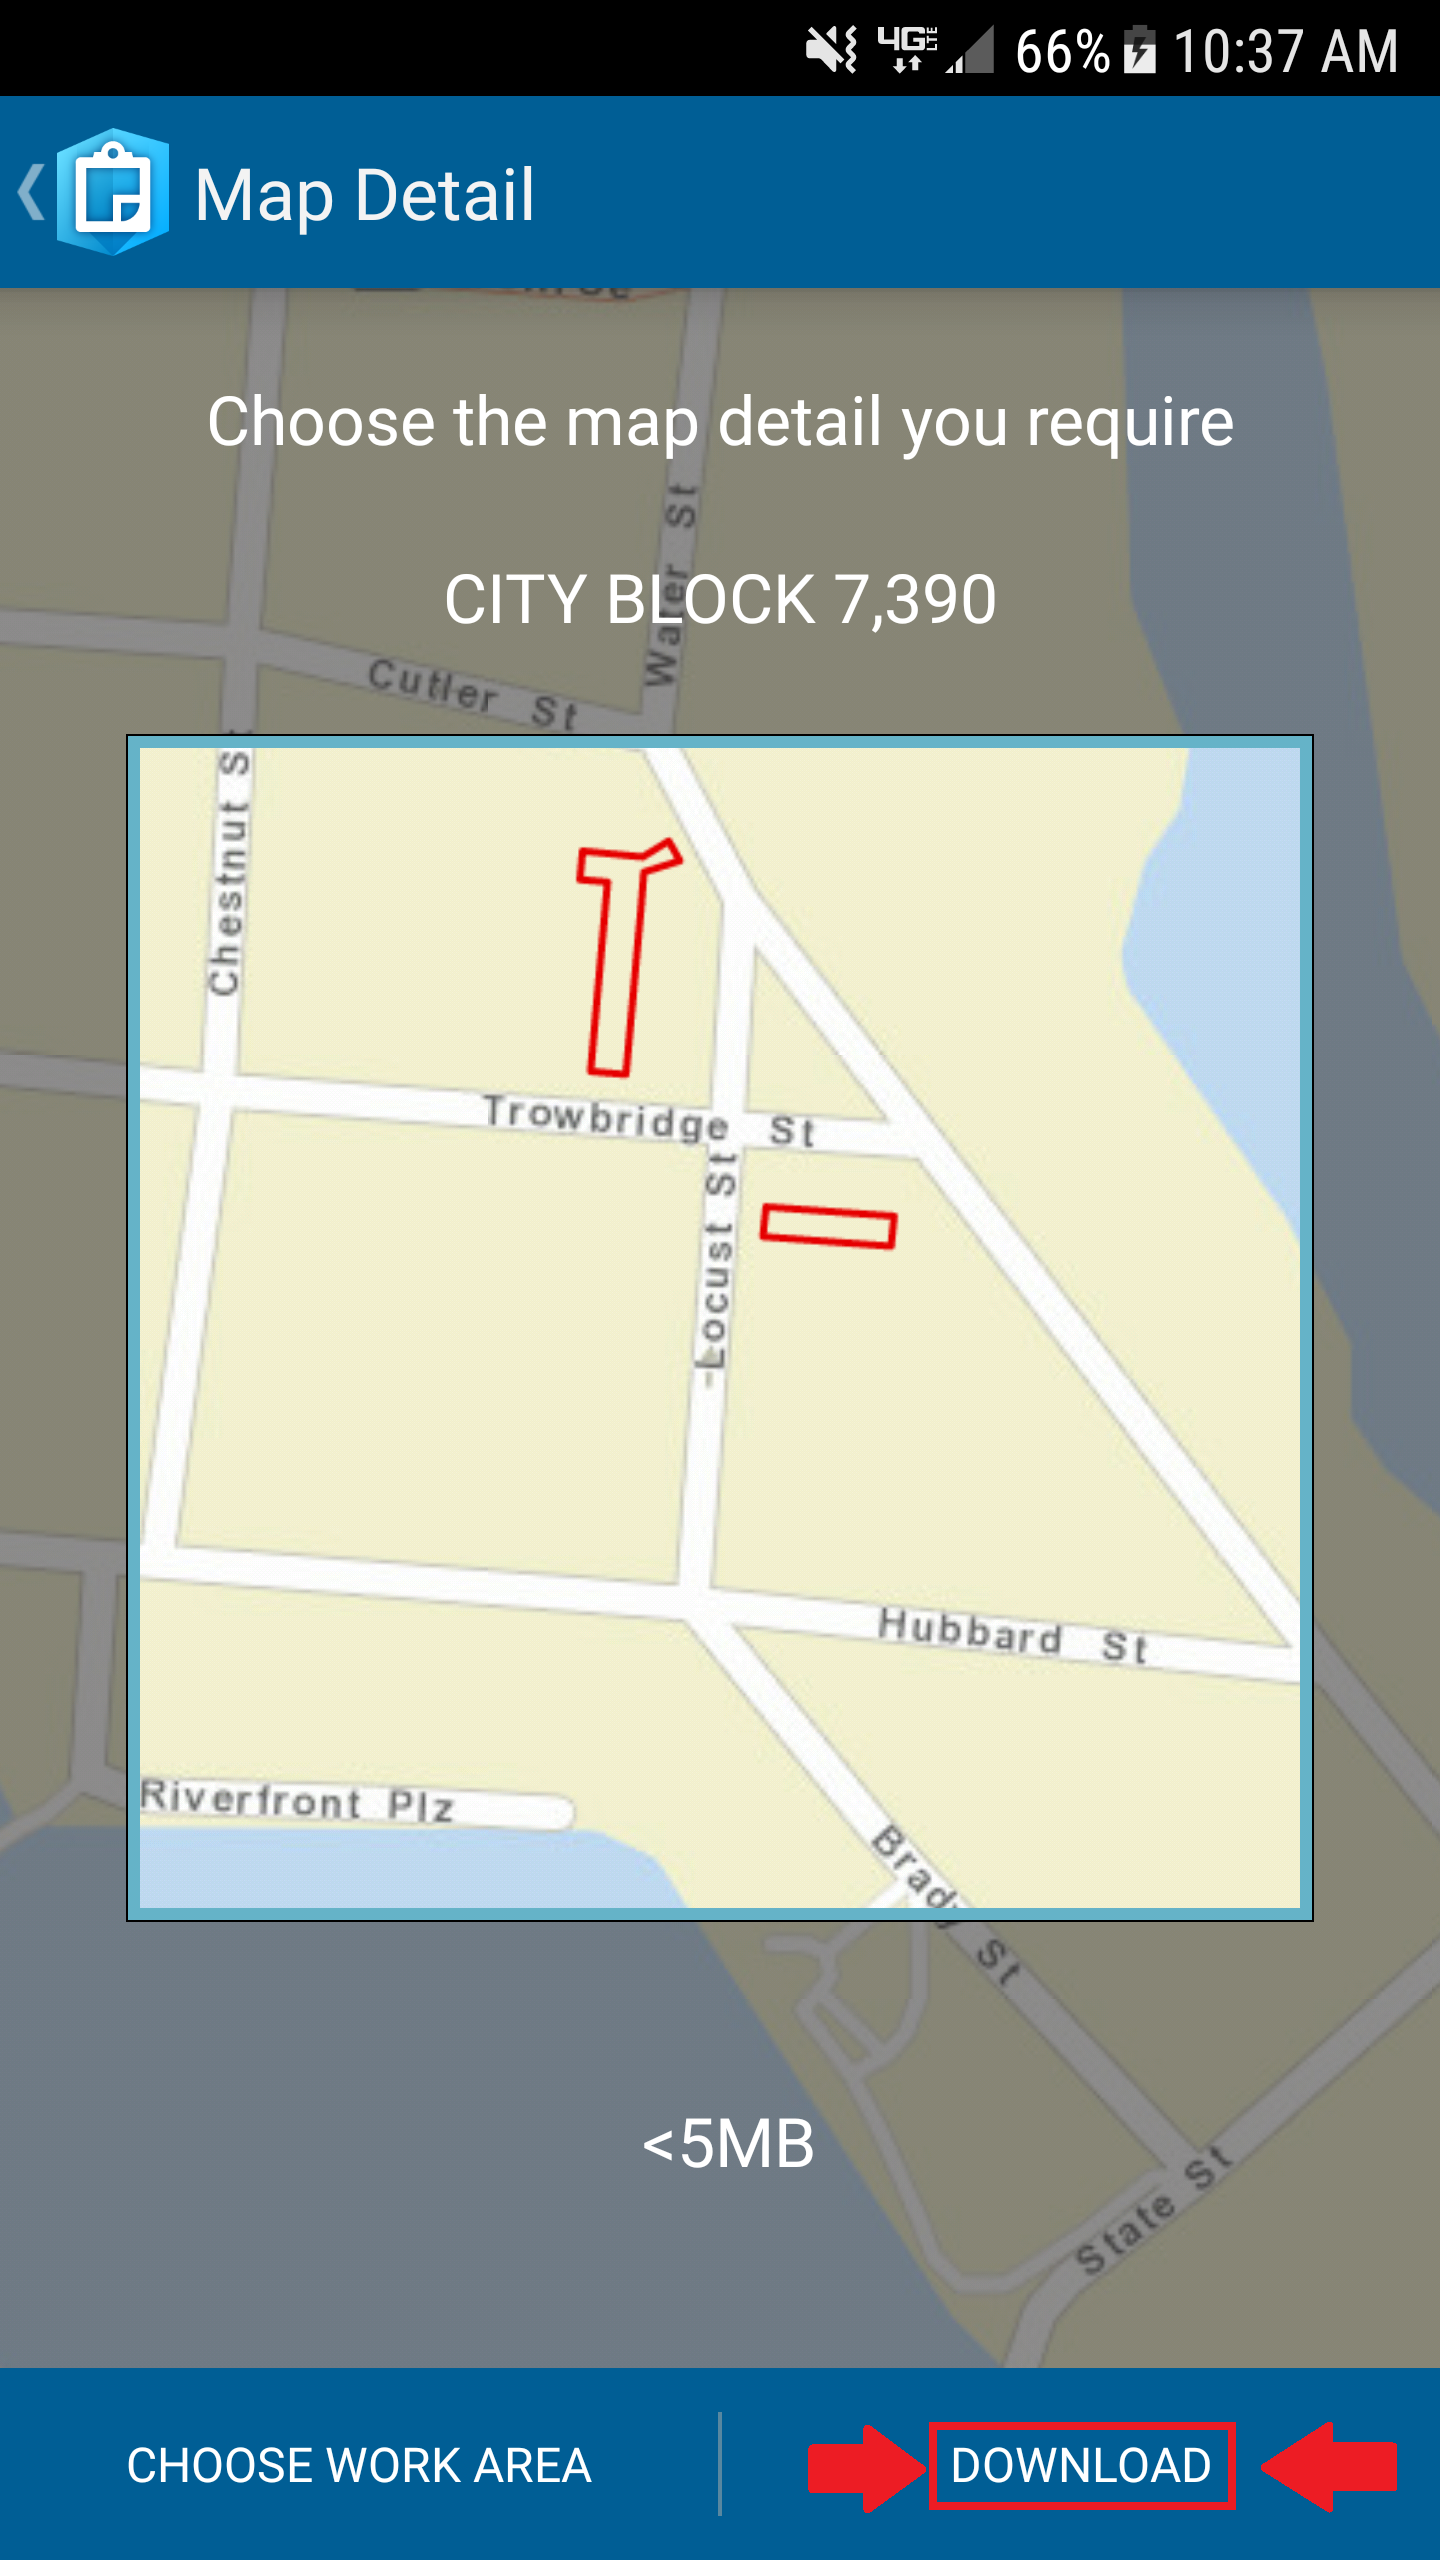
\includegraphics[width=.3\textwidth]{ChooseMapDetail.png}
\caption{Choose Map Detail}
\vspace{.25in}
\HRule \\[.4cm] % Horizontal Line added
\vspace{.25in}
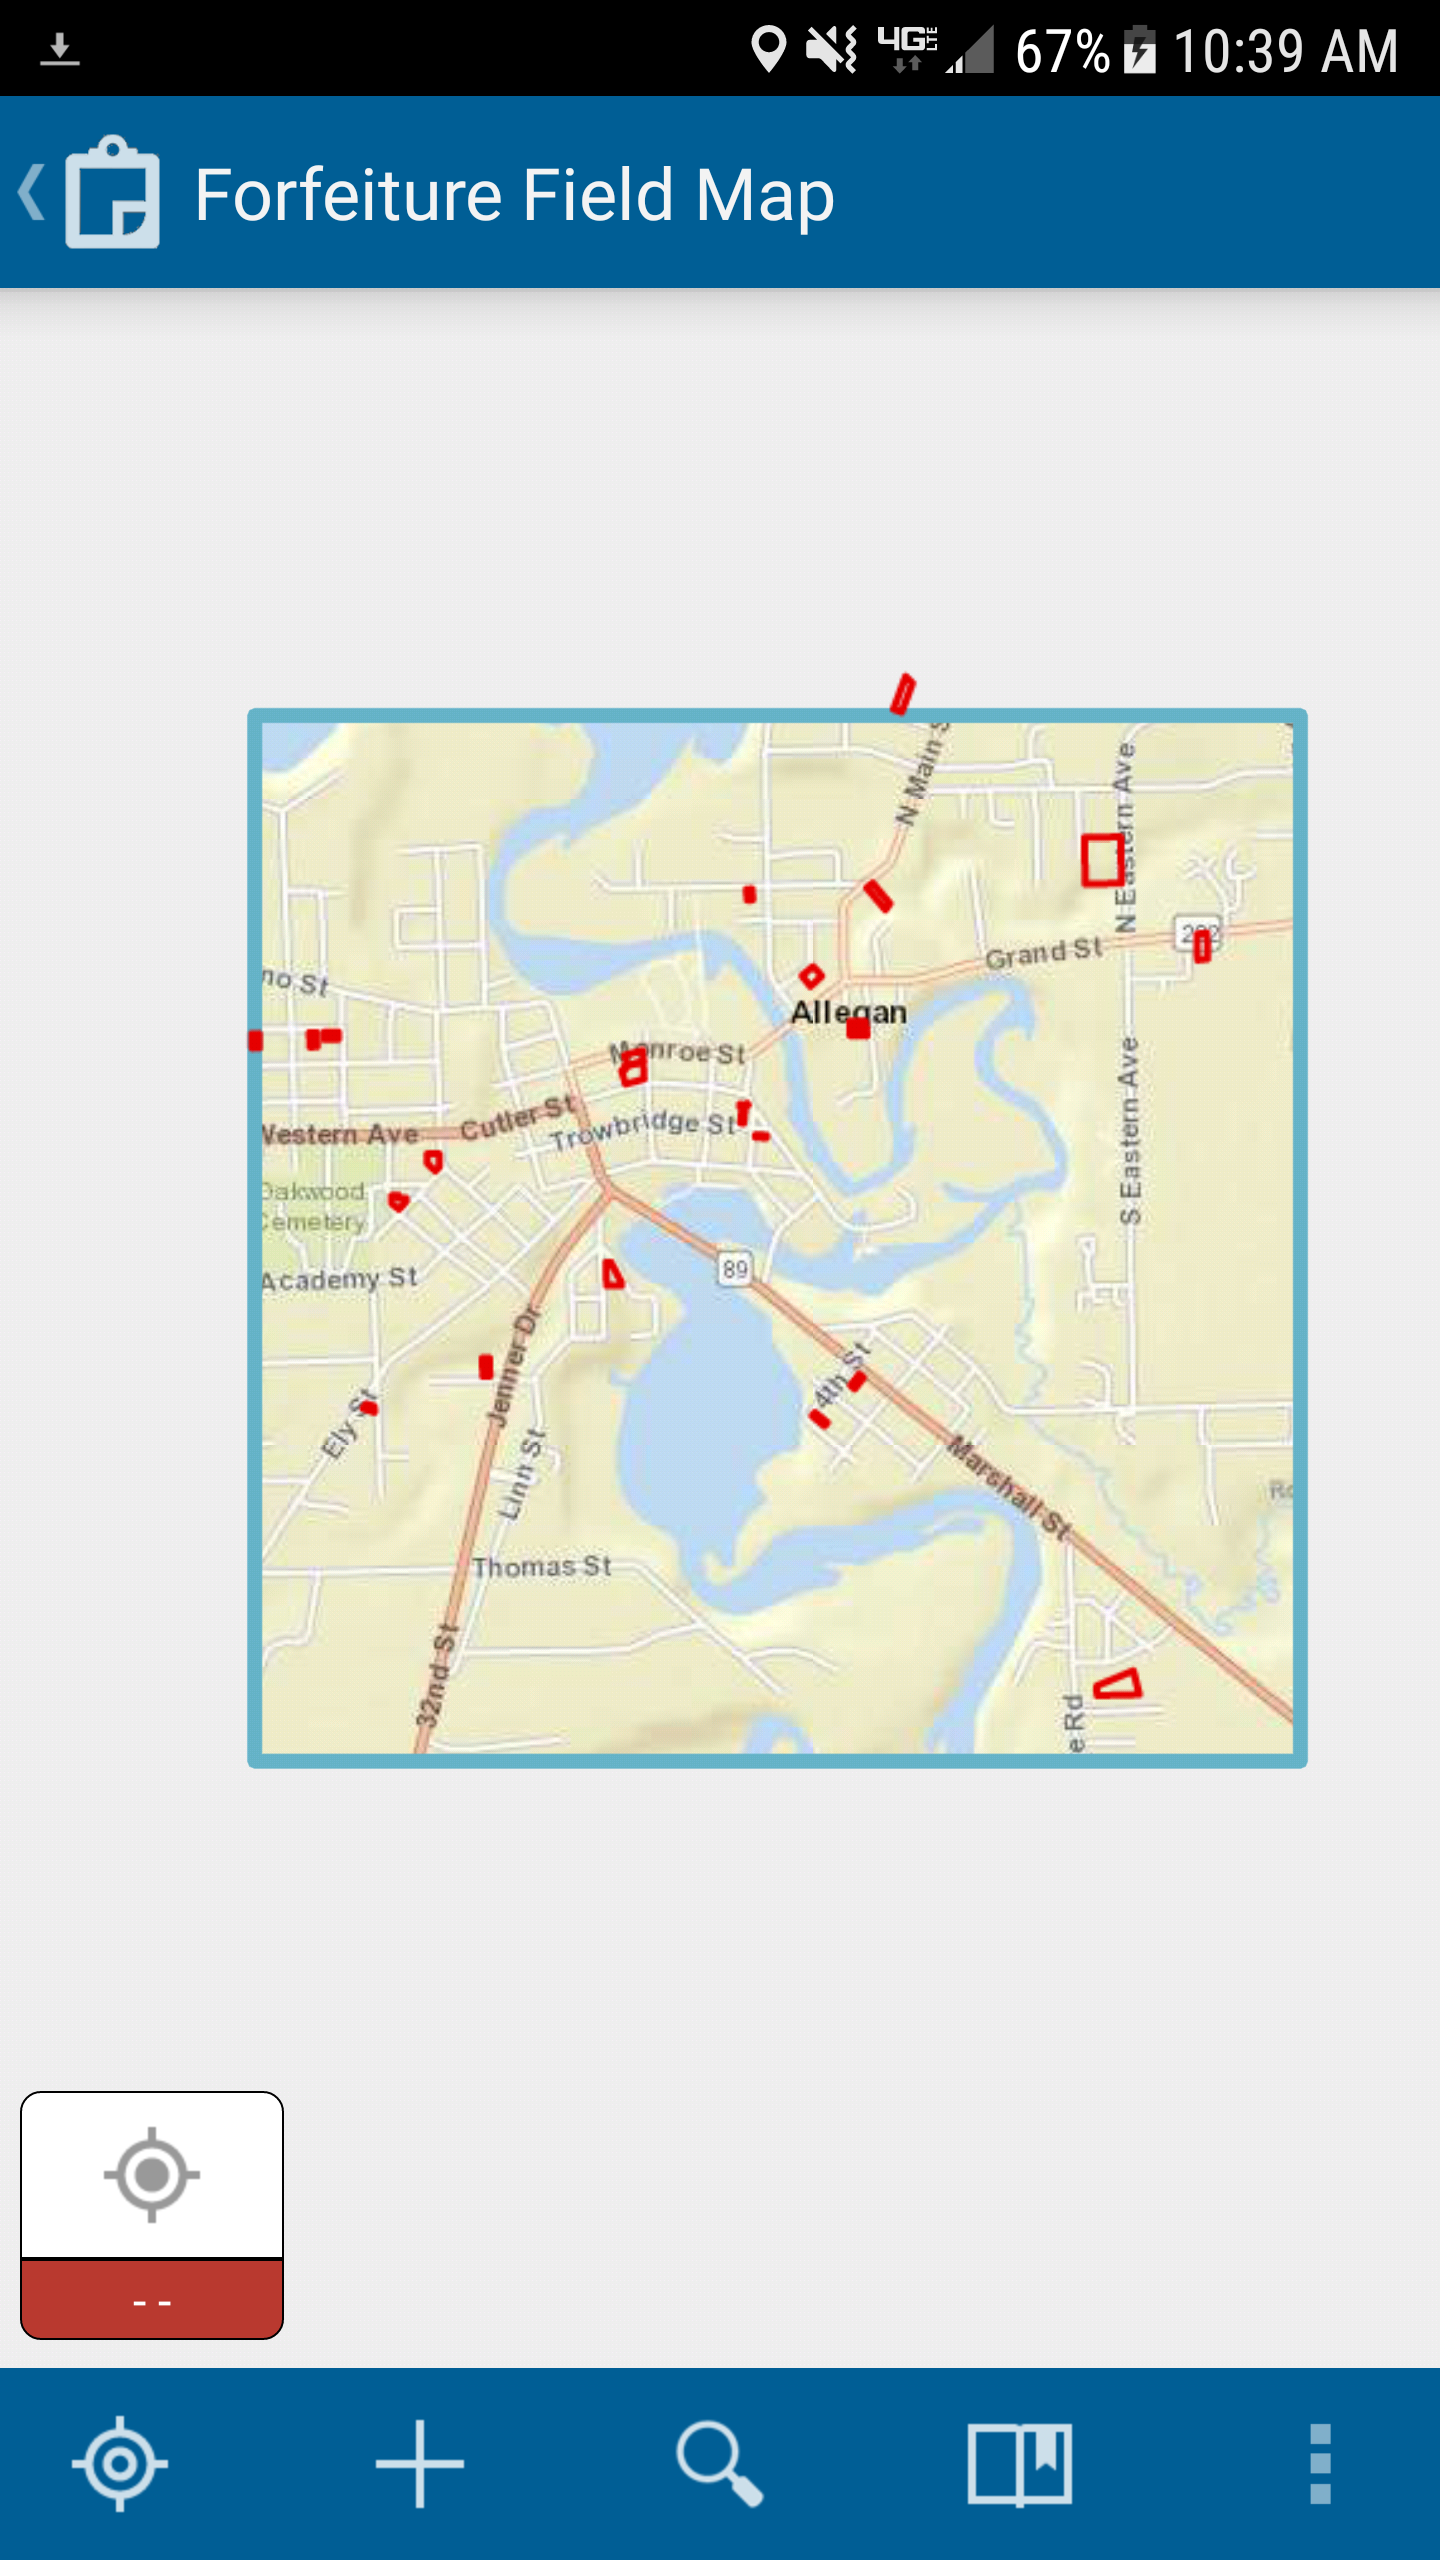
\includegraphics[width=.3\textwidth]{MaponDevice.png}
\caption{Map on Device}
\end{wrapfigure}
Zoom into the level of detail desired.
\vspace{.5in}

\noindent Press Download \\
\vspace{3.5in}

\noindent This area is ready for field data collection.

\clearpage
\paragraph{Open Camera Application Setup Details}

\subparagraph{Install Open Camera}
\begin{itemize}
\item Available from the Google Play Store
\end{itemize}
\begin{figure}[h!]
\centering
    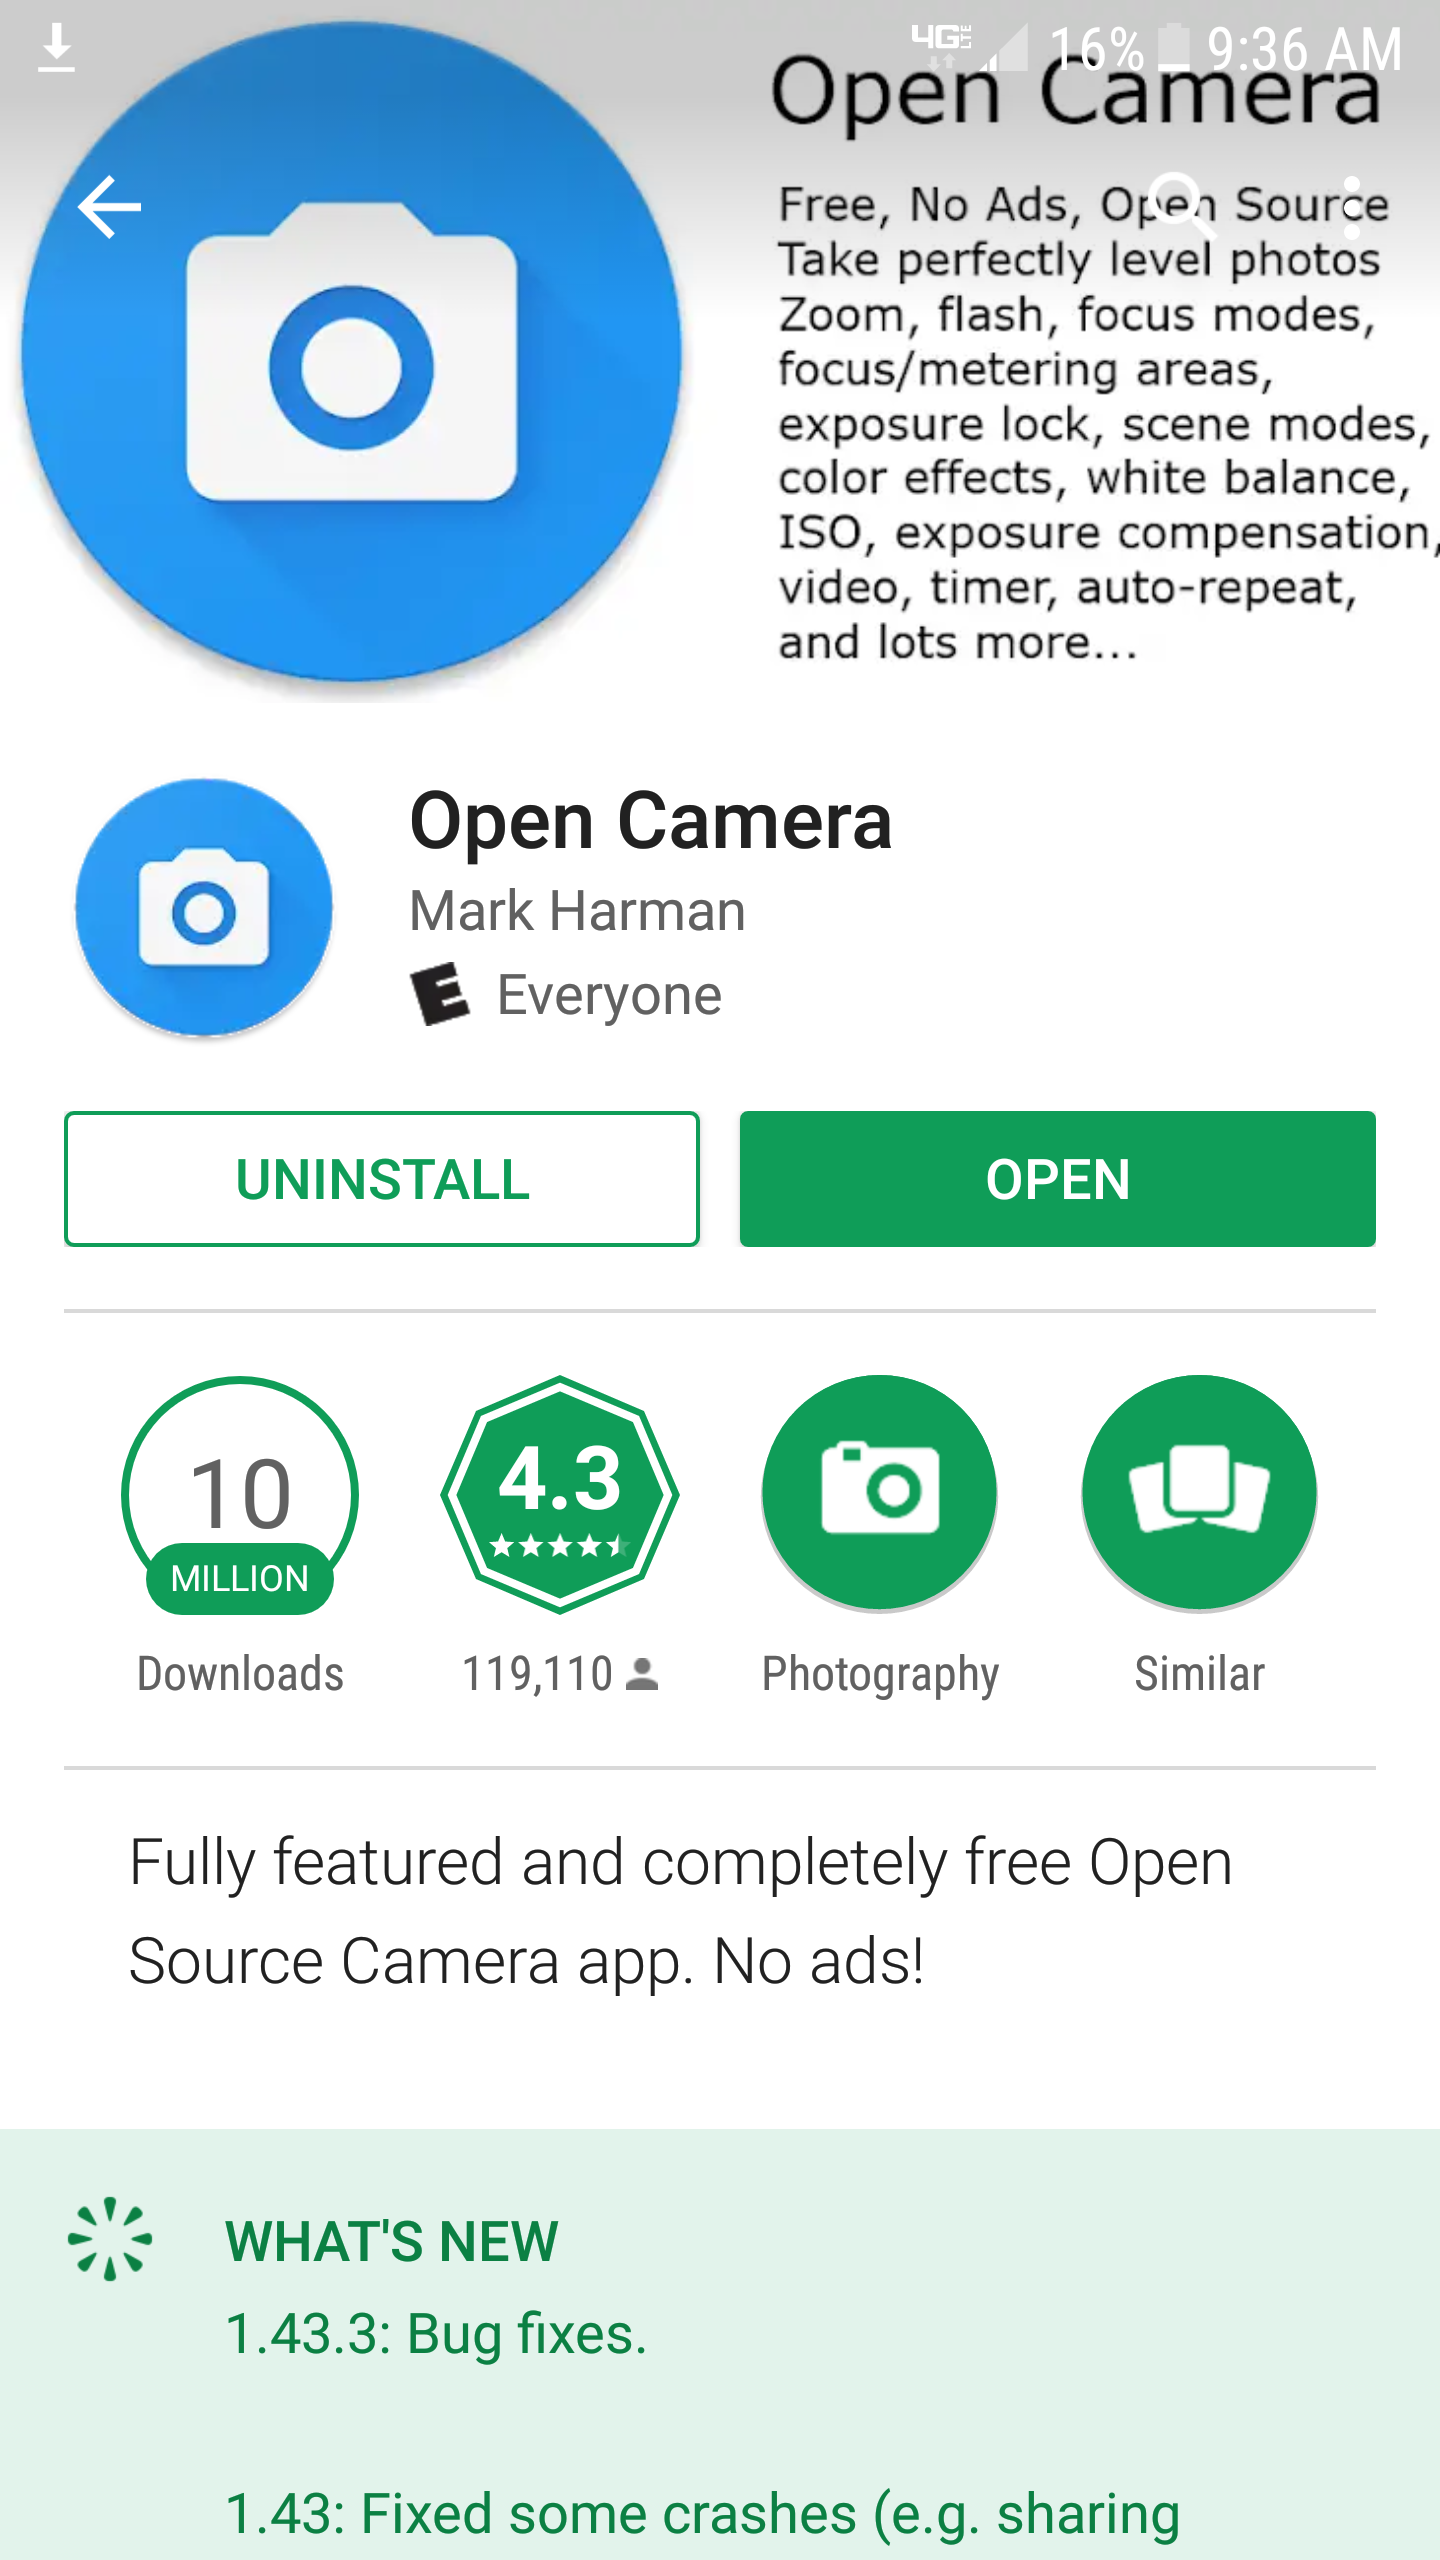
\includegraphics[width=.7\textwidth]{openCameraAppStore.png}
\caption{Open Camera from Google Play Store}
\end{figure}

\clearpage
\subparagraph{Configure Open Camera}

\subparagraph*{\\}
\begin{wrapfigure}{r}{0.5\textwidth}
\centering
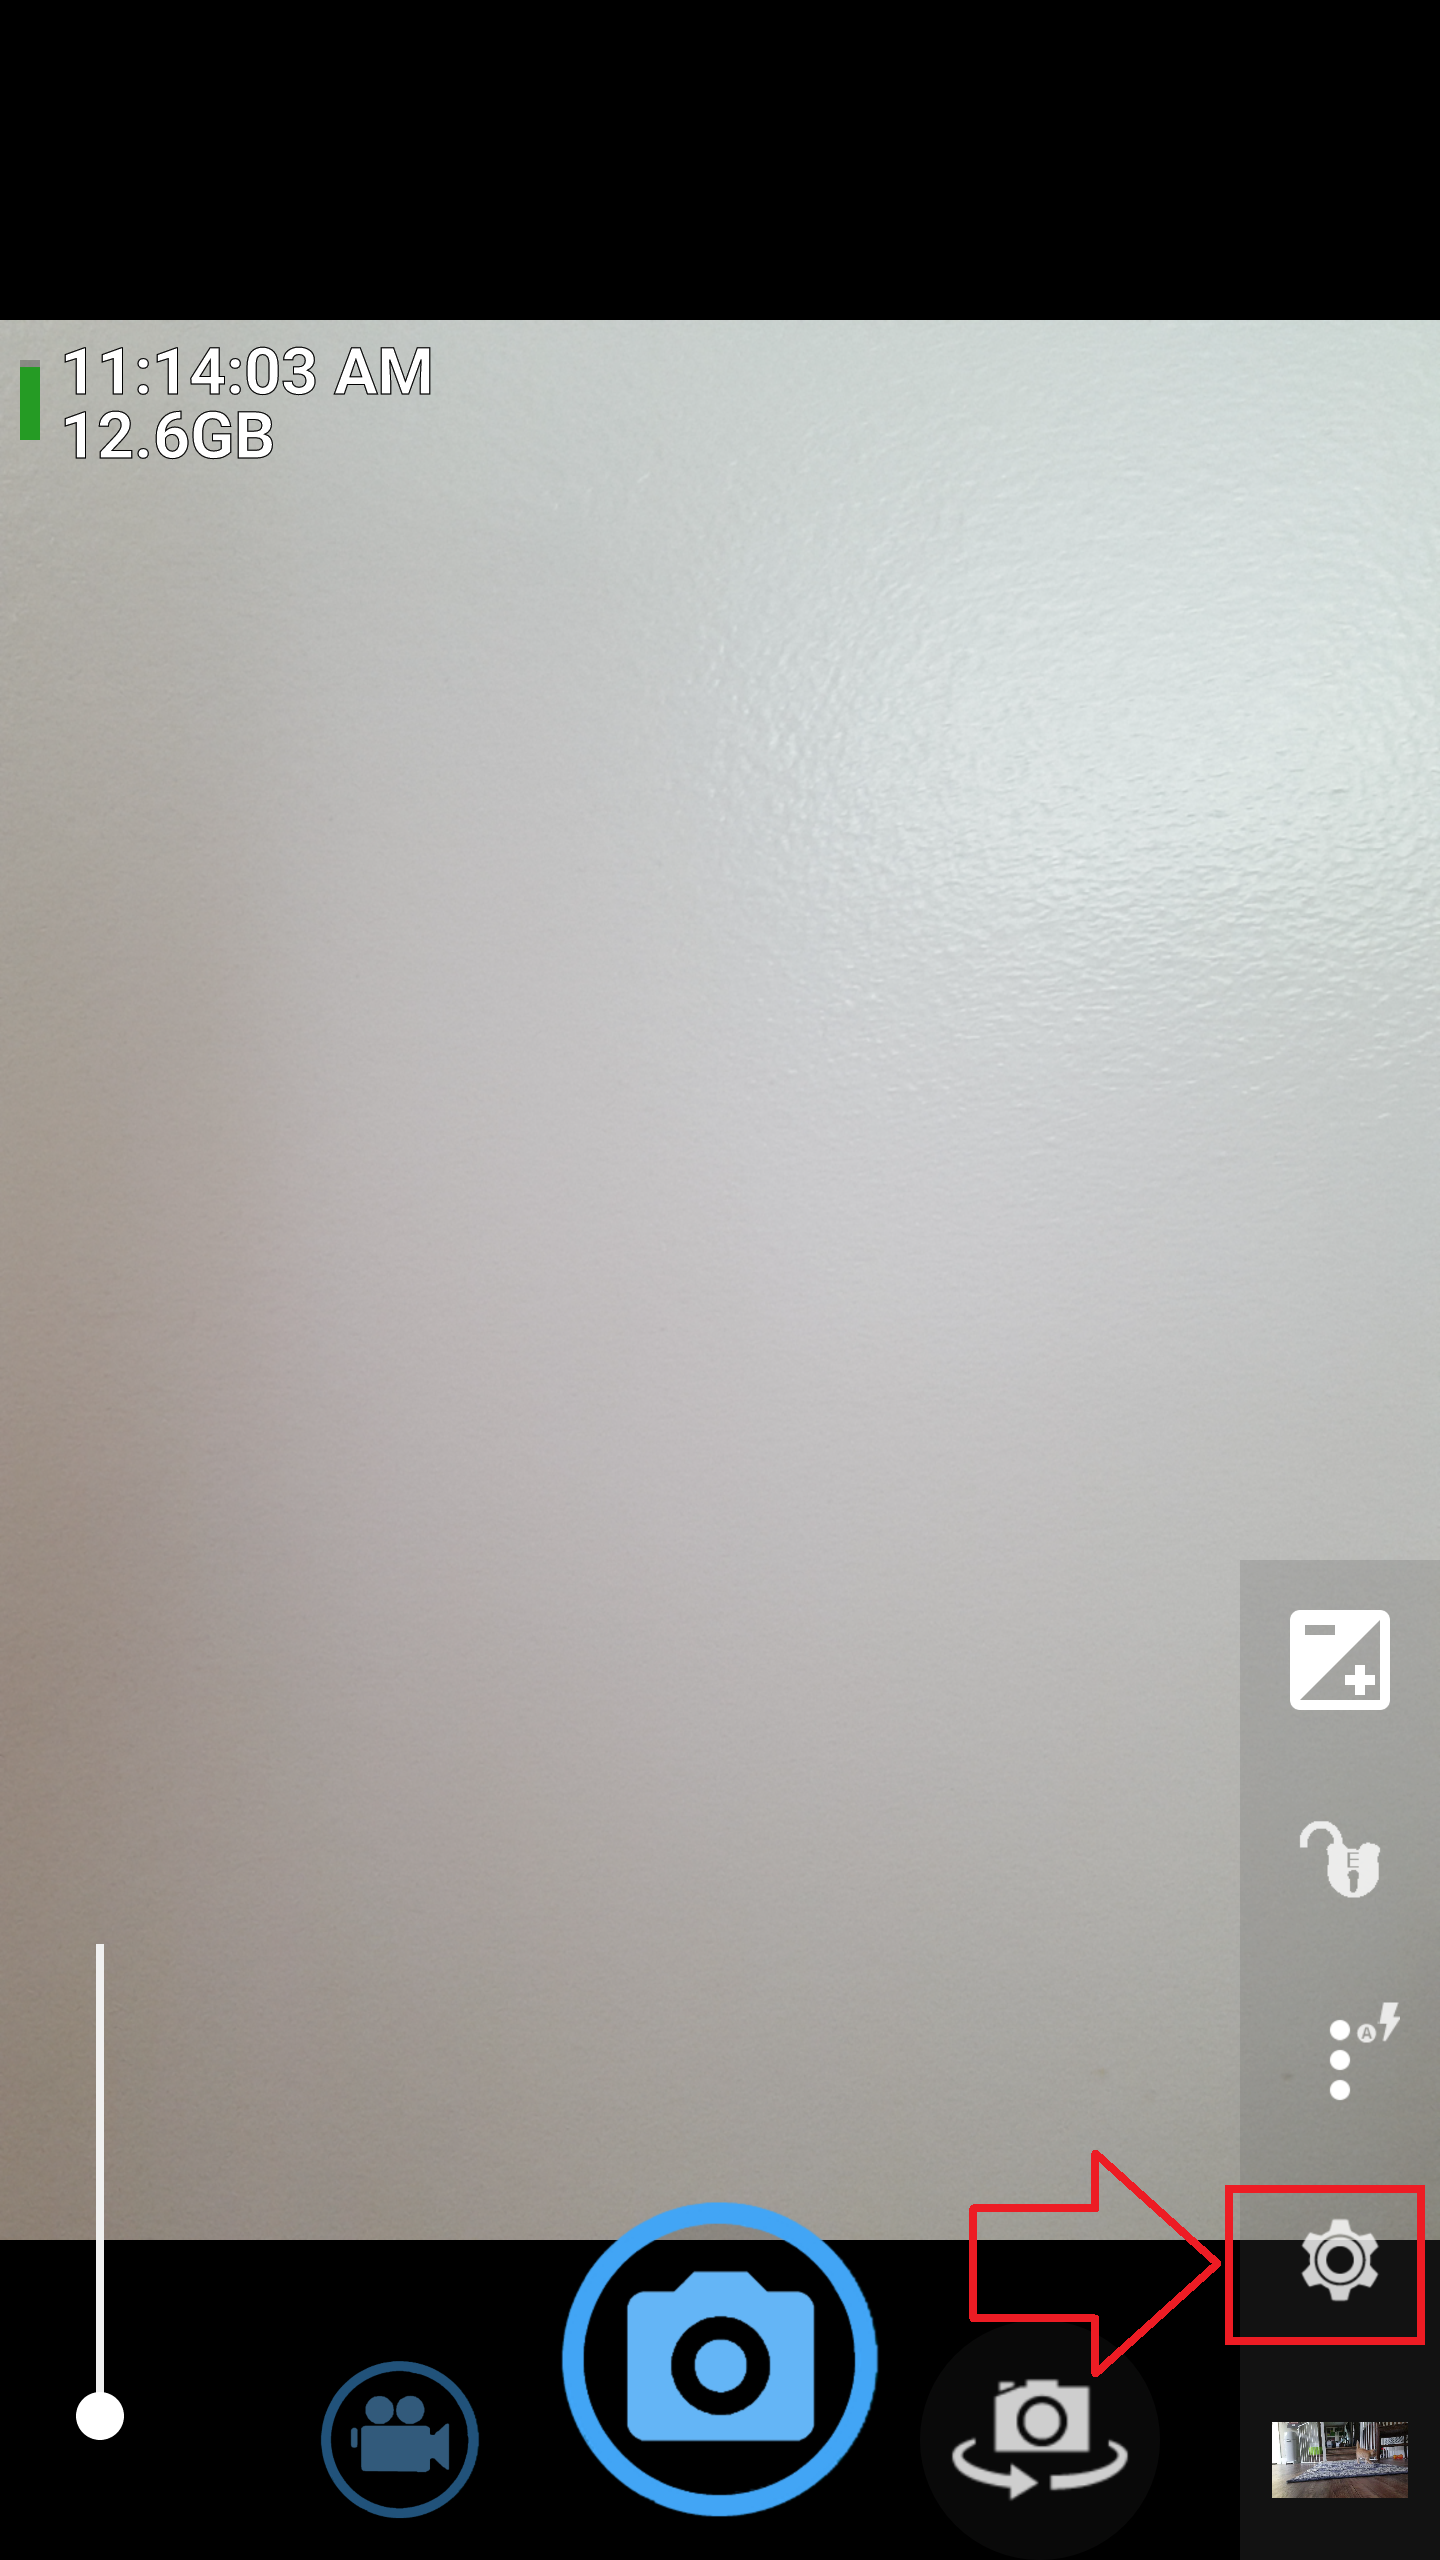
\includegraphics[width=.3\textwidth]{findSettings.png}
\caption{Find Settings Menu}
\vspace{.25in}
\HRule \\[.4cm] % Horizontal Line added
\vspace{.25in}
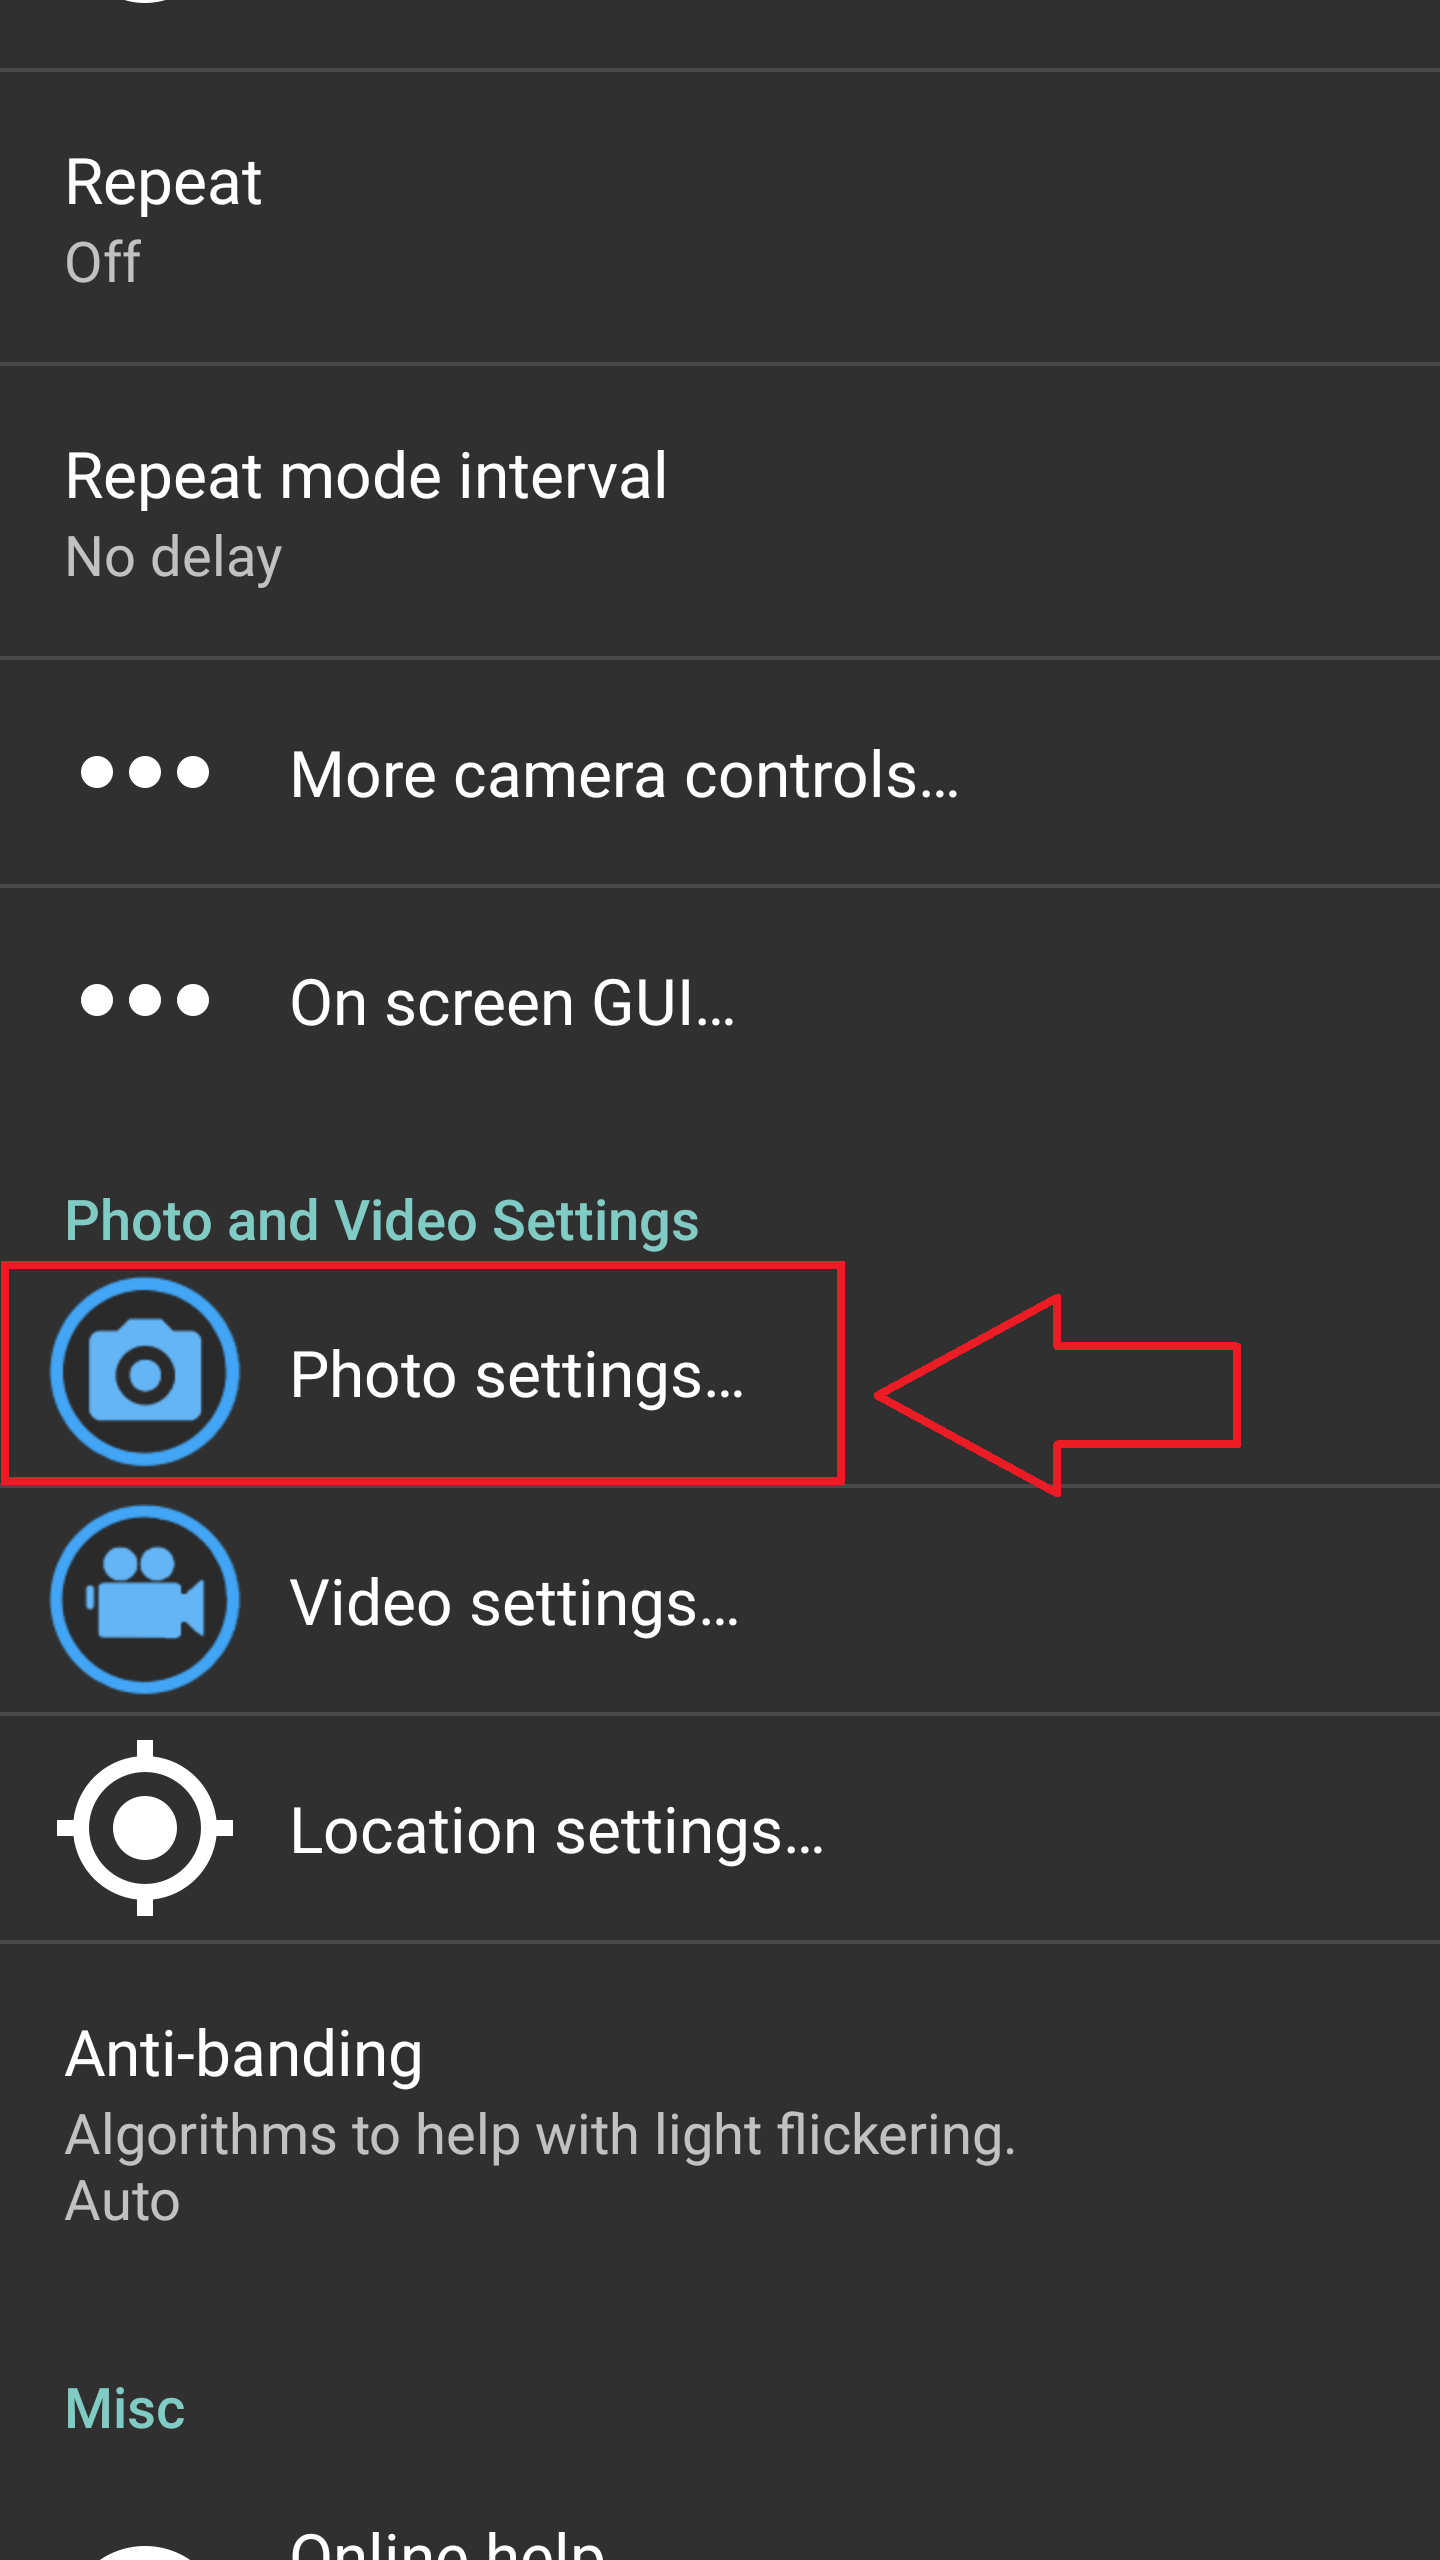
\includegraphics[width=.3\textwidth]{settingsScreen.png}
\caption{Setting Screen}
\end{wrapfigure}
In the Open Camera Application:\\
\vspace{1in}
\noindent Press the gear shaped \Large Settings \normalsize button to go into the settings menu\\
\vspace{3in}
\noindent Press the \Large Photo Settings \normalsize button\\
\clearpage
\subparagraph*{Set Photo Resolution}
\subparagraph*{\\}
\begin{wrapfigure}{r}{0.5\textwidth}
\centering
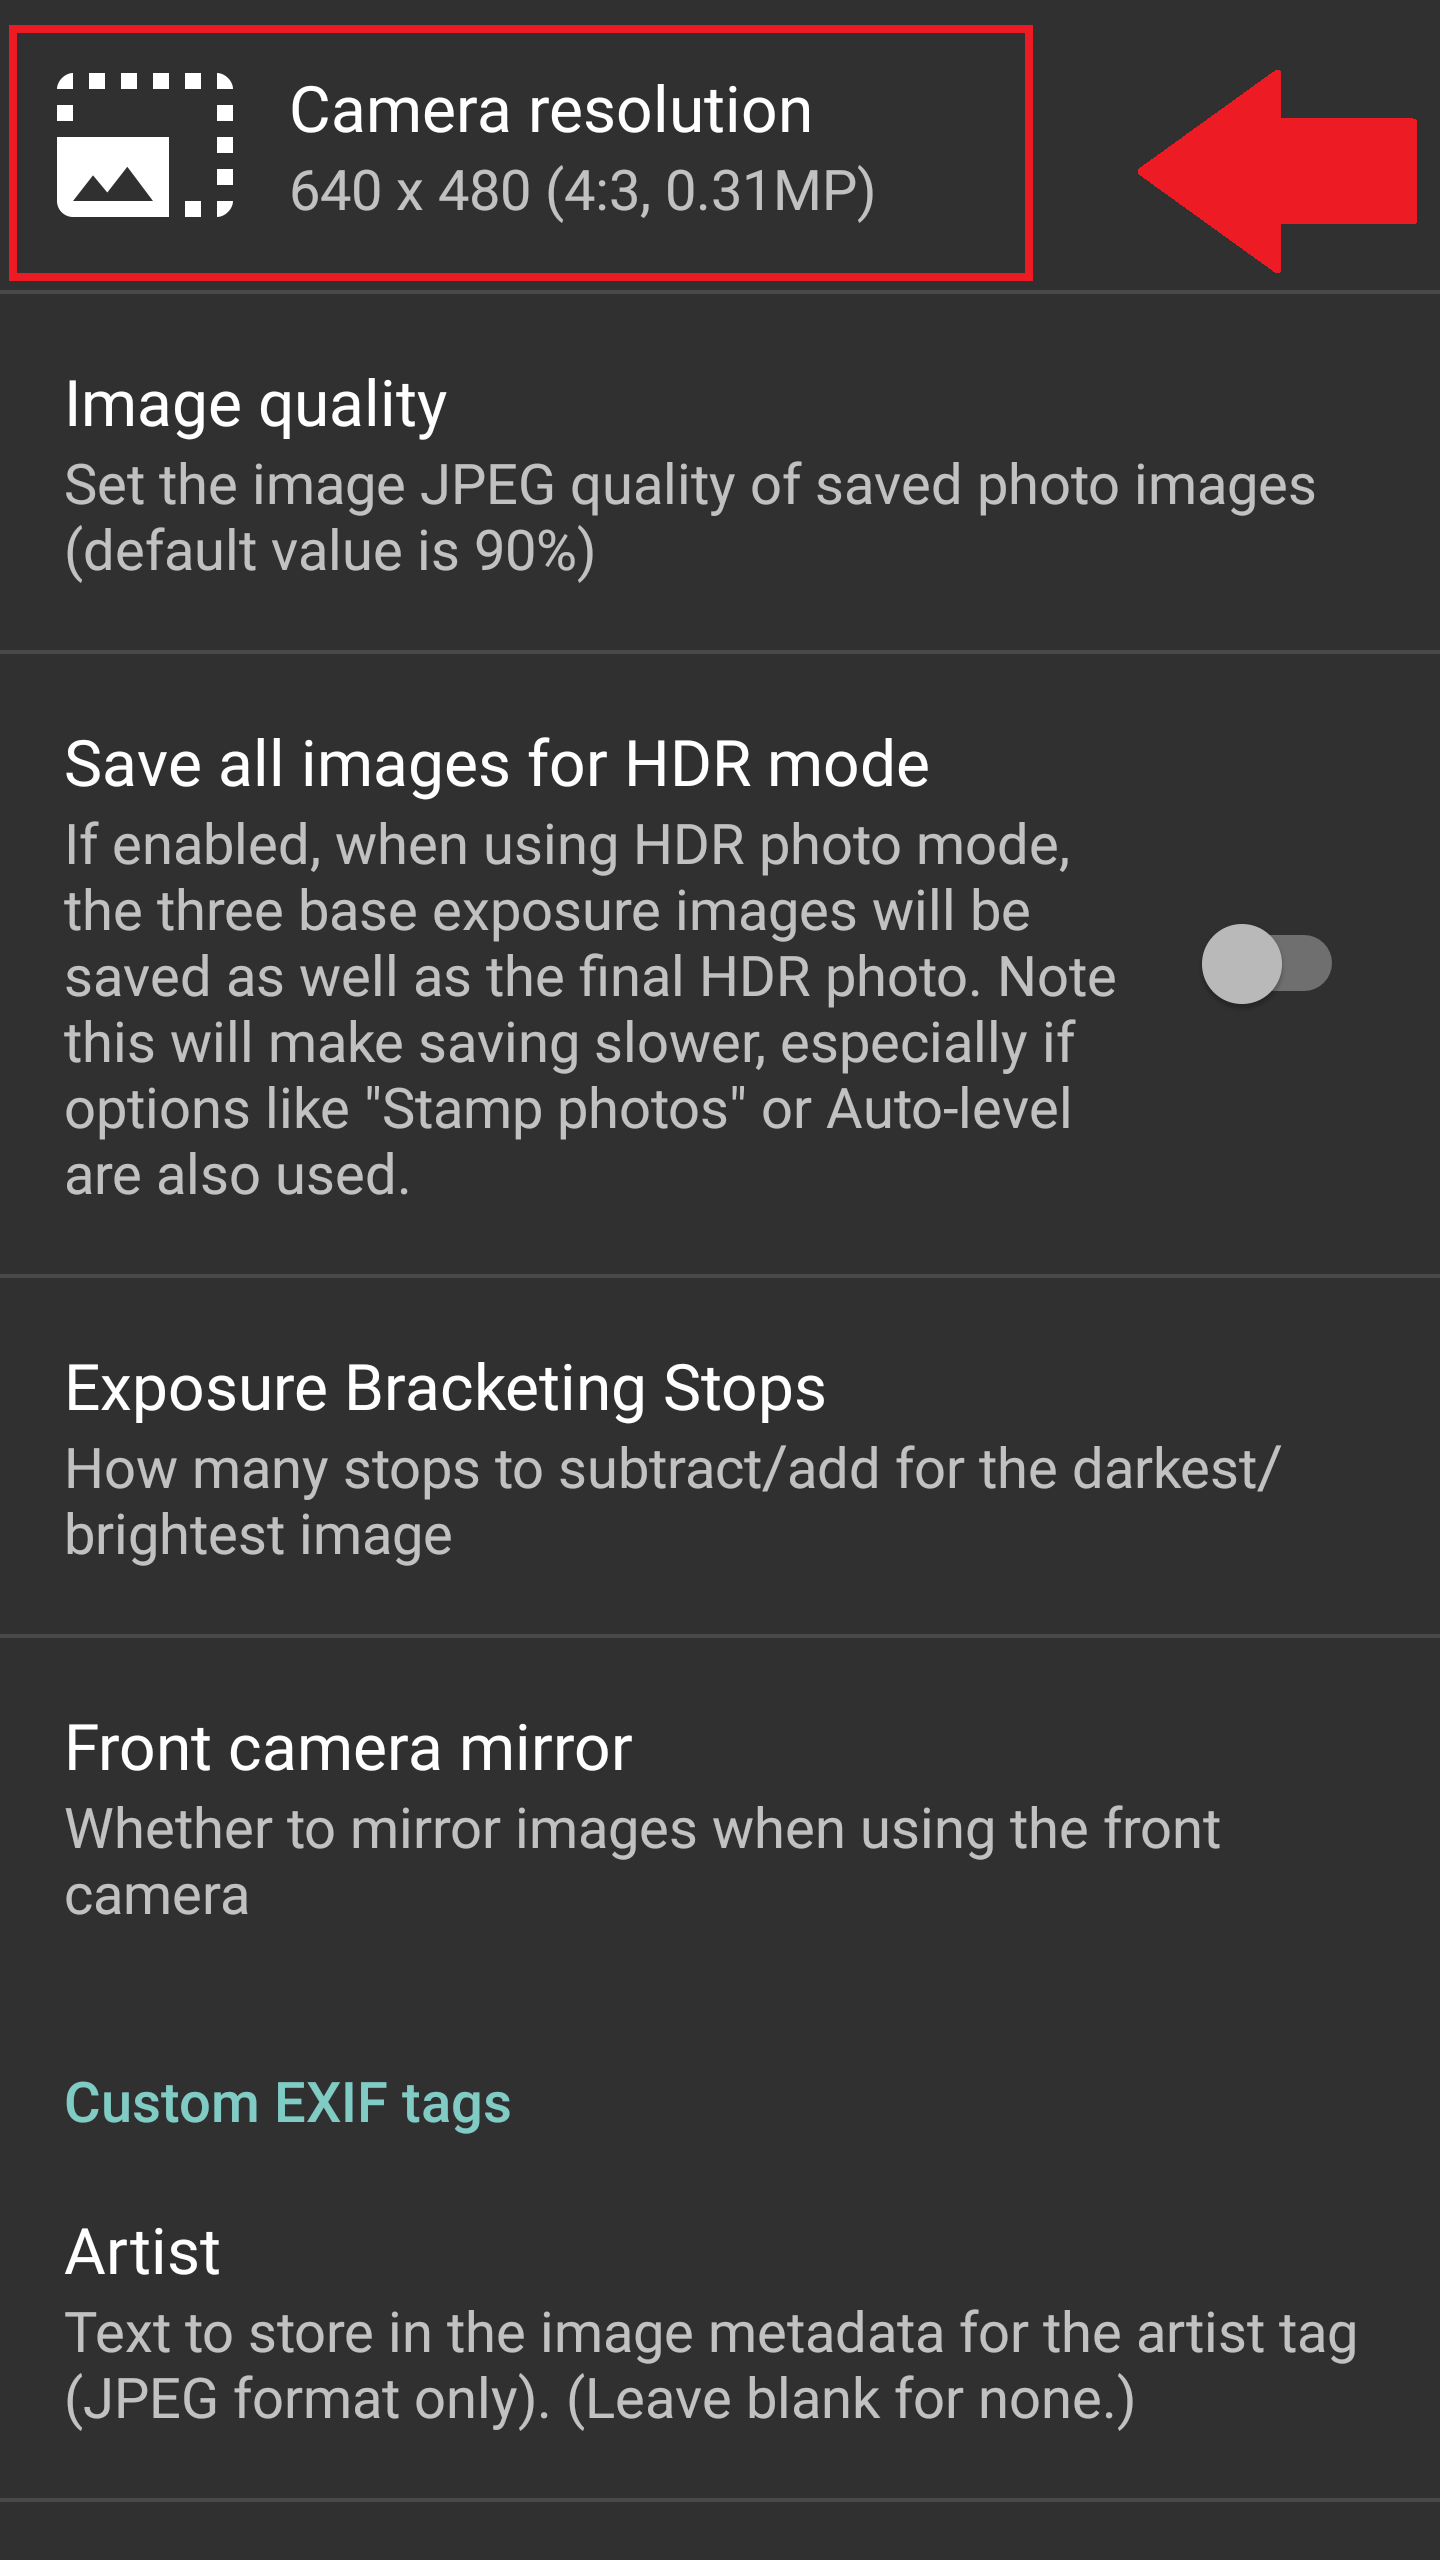
\includegraphics[width=.3\textwidth]{photoSettings.png}
\caption{Photo Settings Menu}
\vspace{.25in}
\HRule \\[.4cm] % Horizontal Line added
\vspace{.25in}
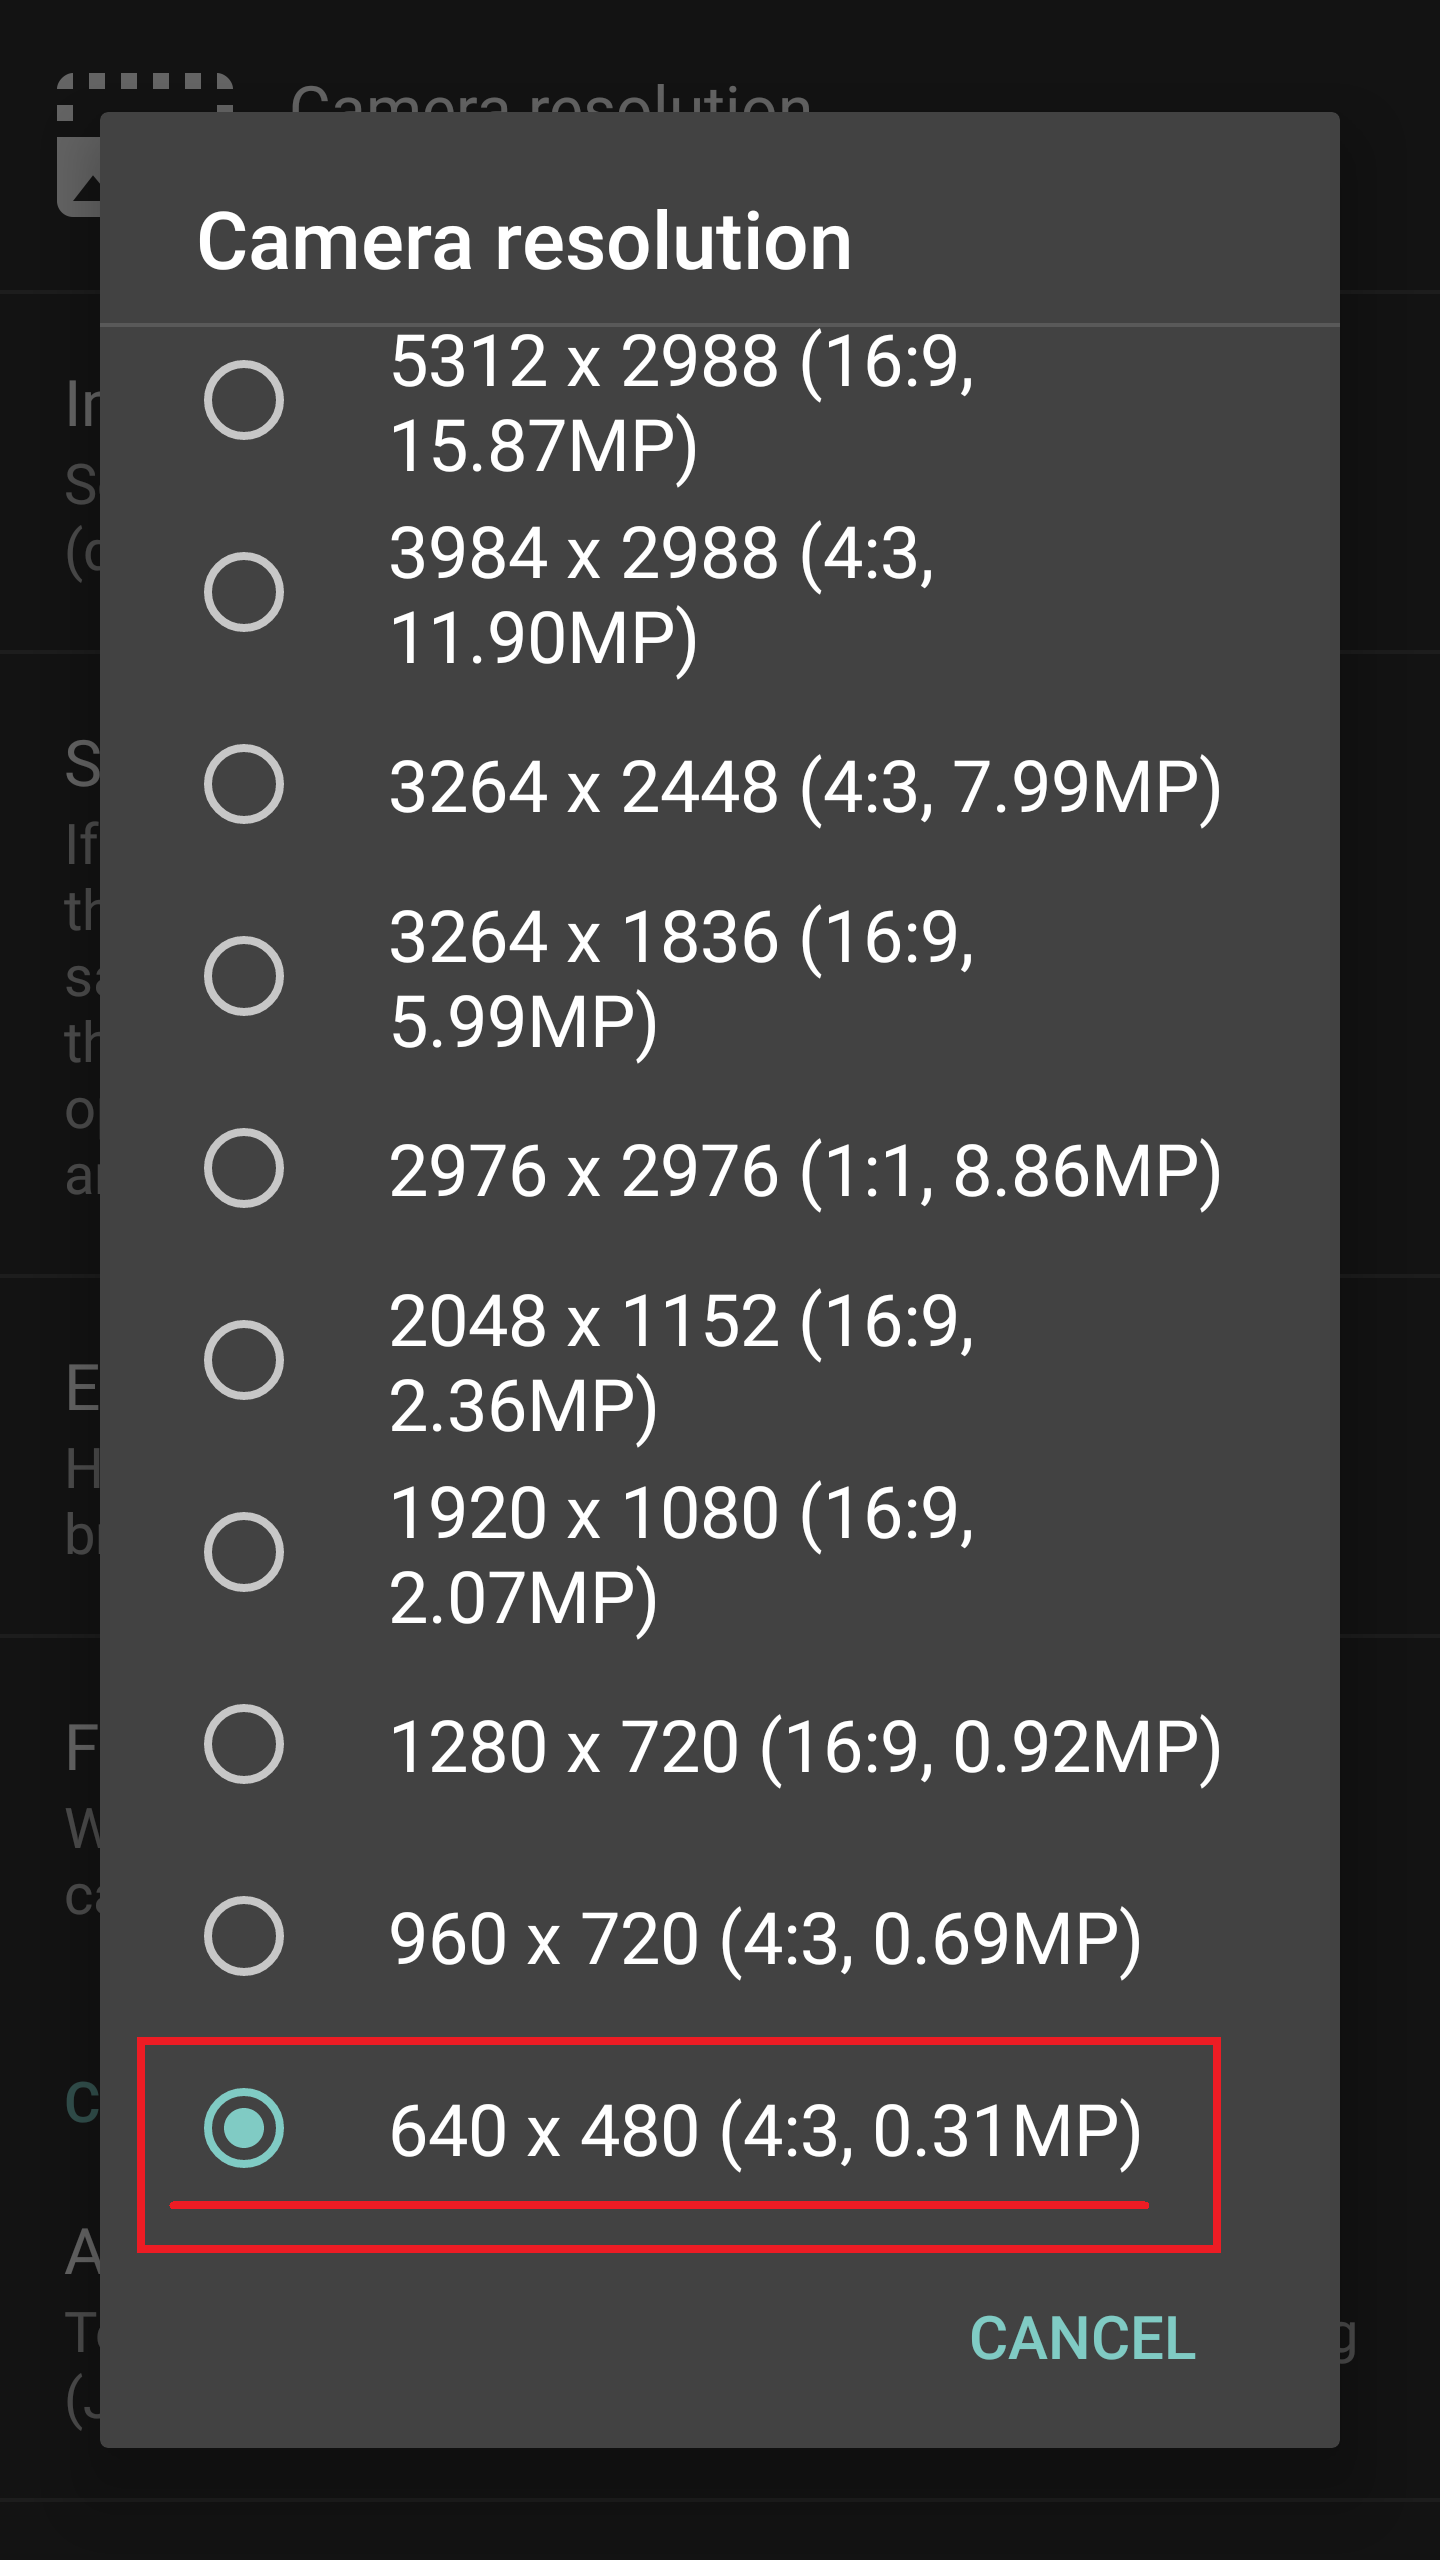
\includegraphics[width=.3\textwidth]{cameraResolutionSetting.png}
\caption{Camera Resolution Setting}
\end{wrapfigure}
In \Large photo settings:\\
\vspace{1in}
\noindent Press the \Large Camera resolution \normalsize button\\
\vspace{3in}
\noindent Select \textbf{\LARGE 640 x 480}\\
\clearpage
\paragraph{Daily Preprocessing Routine}
\subparagraph{Execute Preprocessing Script}A tool in ArcGIS that:
\begin{itemize}
\item Exports current forfeiture list from BSA
\item Updates webmap layers with results from BSA export
\end{itemize}
\subparagraph*{\\}
\begin{wrapfigure}{r}{0.75\textwidth}
\centering
\includegraphics[width=.65\textwidth]{preprocess.png}
\caption{Processing Tools}
\end{wrapfigure}
In Catalog:\\
\vspace{1in}
\noindent Open the toolbox\\
\vspace{1in}
\noindent Open tool 1\\
\clearpage
\subparagraph{Synchronize the Forfeiture Field Map\\}
\subparagraph*{\texorpdfstring{\\}{}}
\begin{wrapfigure}{r}{0.5\textwidth}
\centering
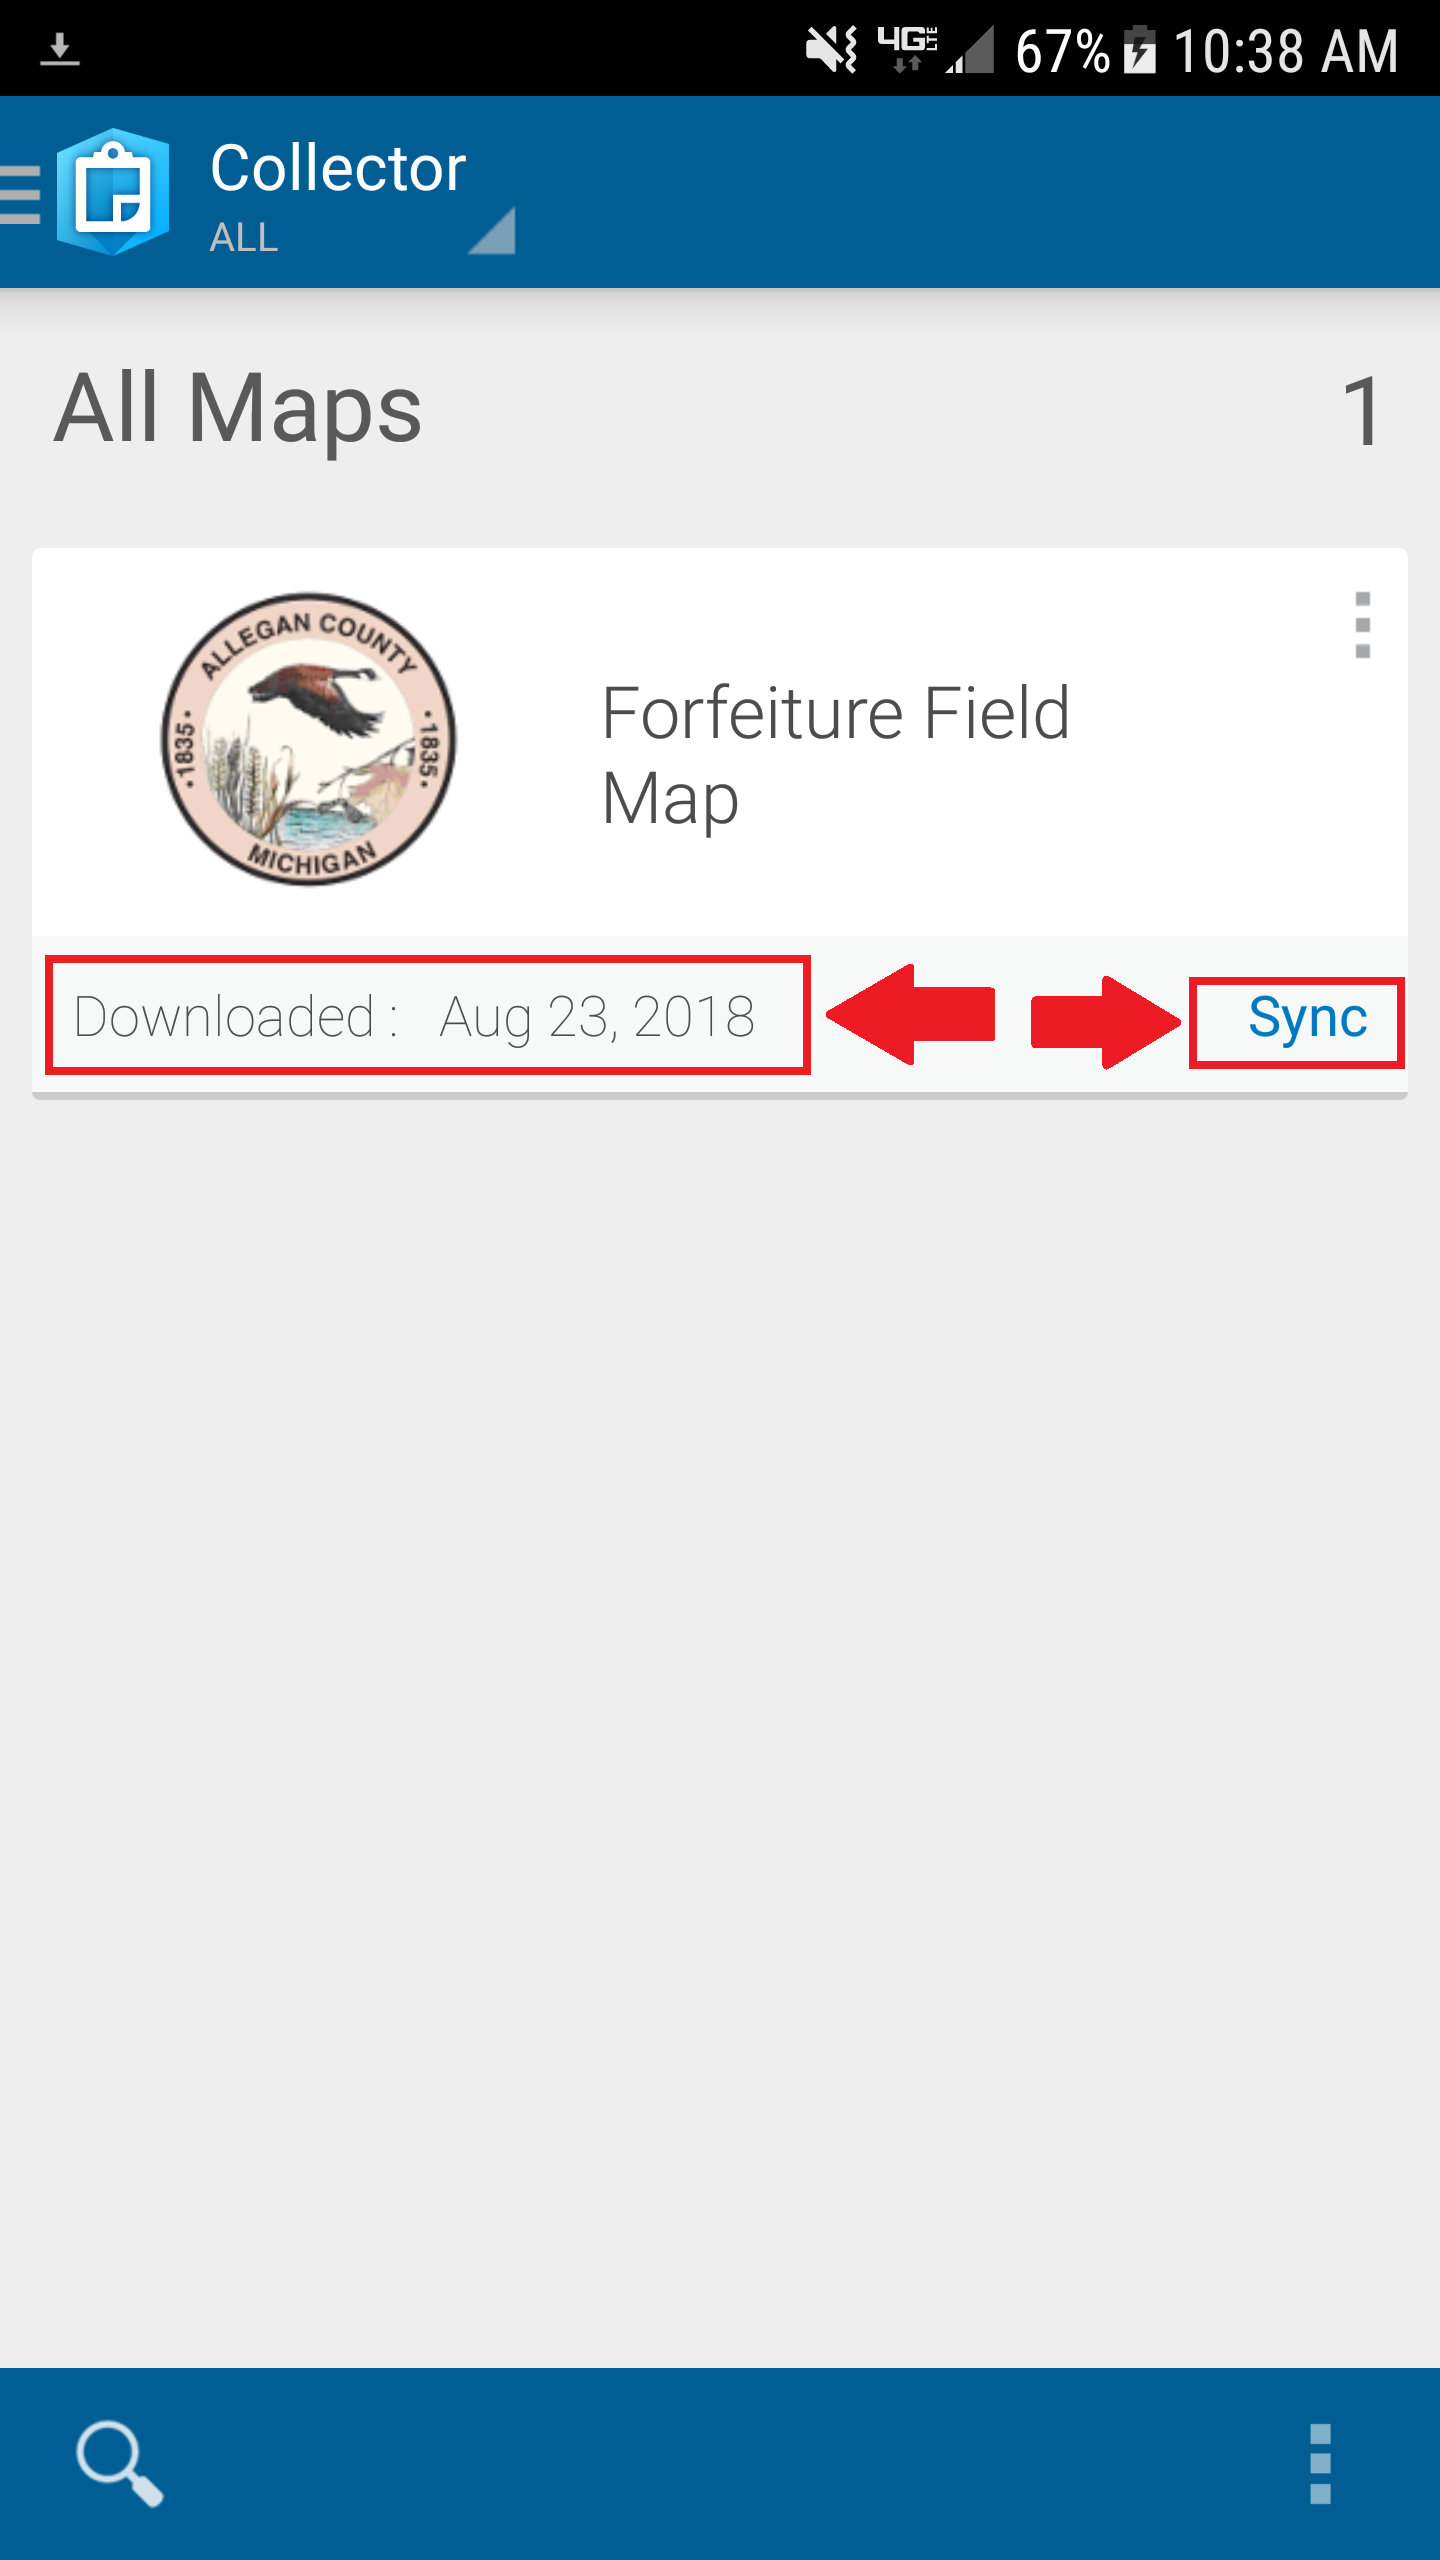
\includegraphics[width=.3\textwidth]{MapDownloaded.png}
\caption{Map Downloaded}
\vspace{.25in}
\HRule \\[.4cm] % Horizontal Line added
\vspace{.25in}
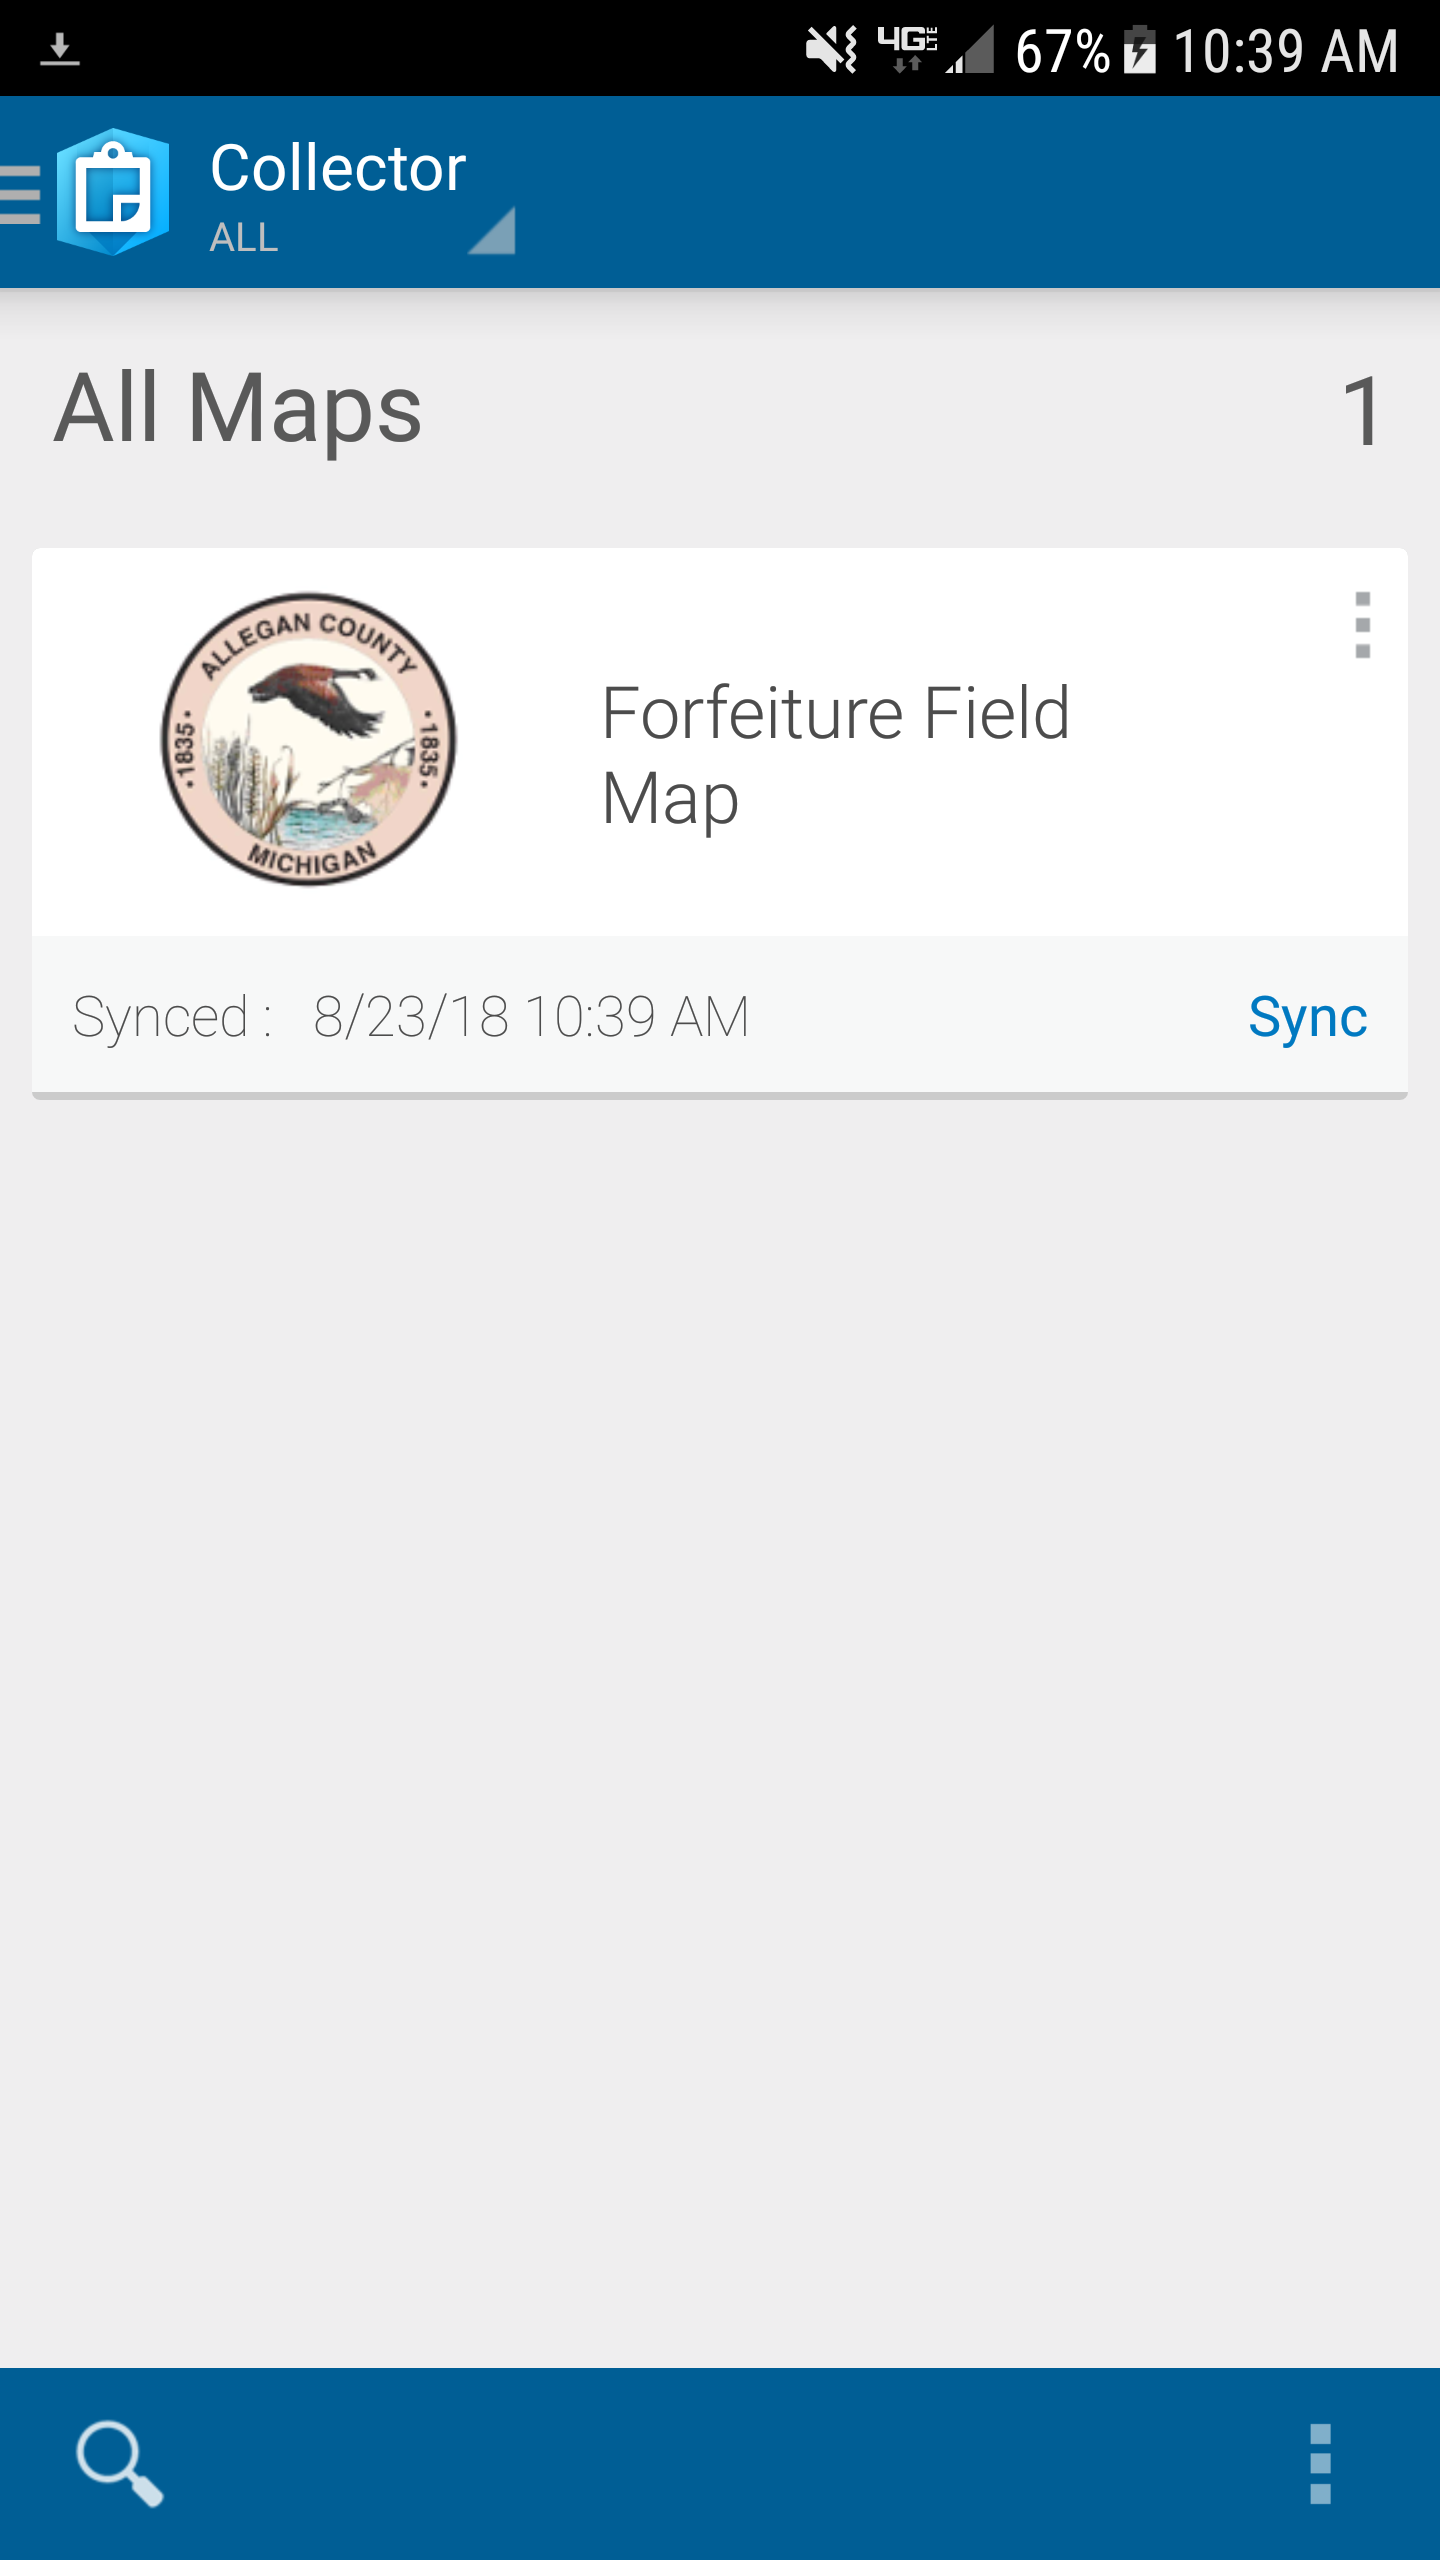
\includegraphics[width=.3\textwidth]{MapSyncronized.png}
\caption{Map Synchronized}
\end{wrapfigure}
\Large Note the date and time:
\vspace{1.5in}
\noindent Press \Large Sync
\vspace{1.5in}
\Large Note the date and time
\vspace{1.5in}
Map is now synchronized
\clearpage
\paragraph{Forfeiture Data Collection}
\subparagraph{Forfeiture Parcels Data Details}
Attributes are of four entry types:\begin{itemize}
\item prefilled
\item autofill
\item dropdown
\item text box \end{itemize}
For each site visited, select the desired parcel, push the edit button and collect attributes.  If the boxes are autofill, select from dropdown or typed.\bigskip 
\clearpage
\subparagraph{Device 1 Field Operation}Device one data collection interface, used to add data to all of the boxes
\subparagraph*{\\}
\begin{wrapfigure}{r}{0.5\textwidth}
\centering
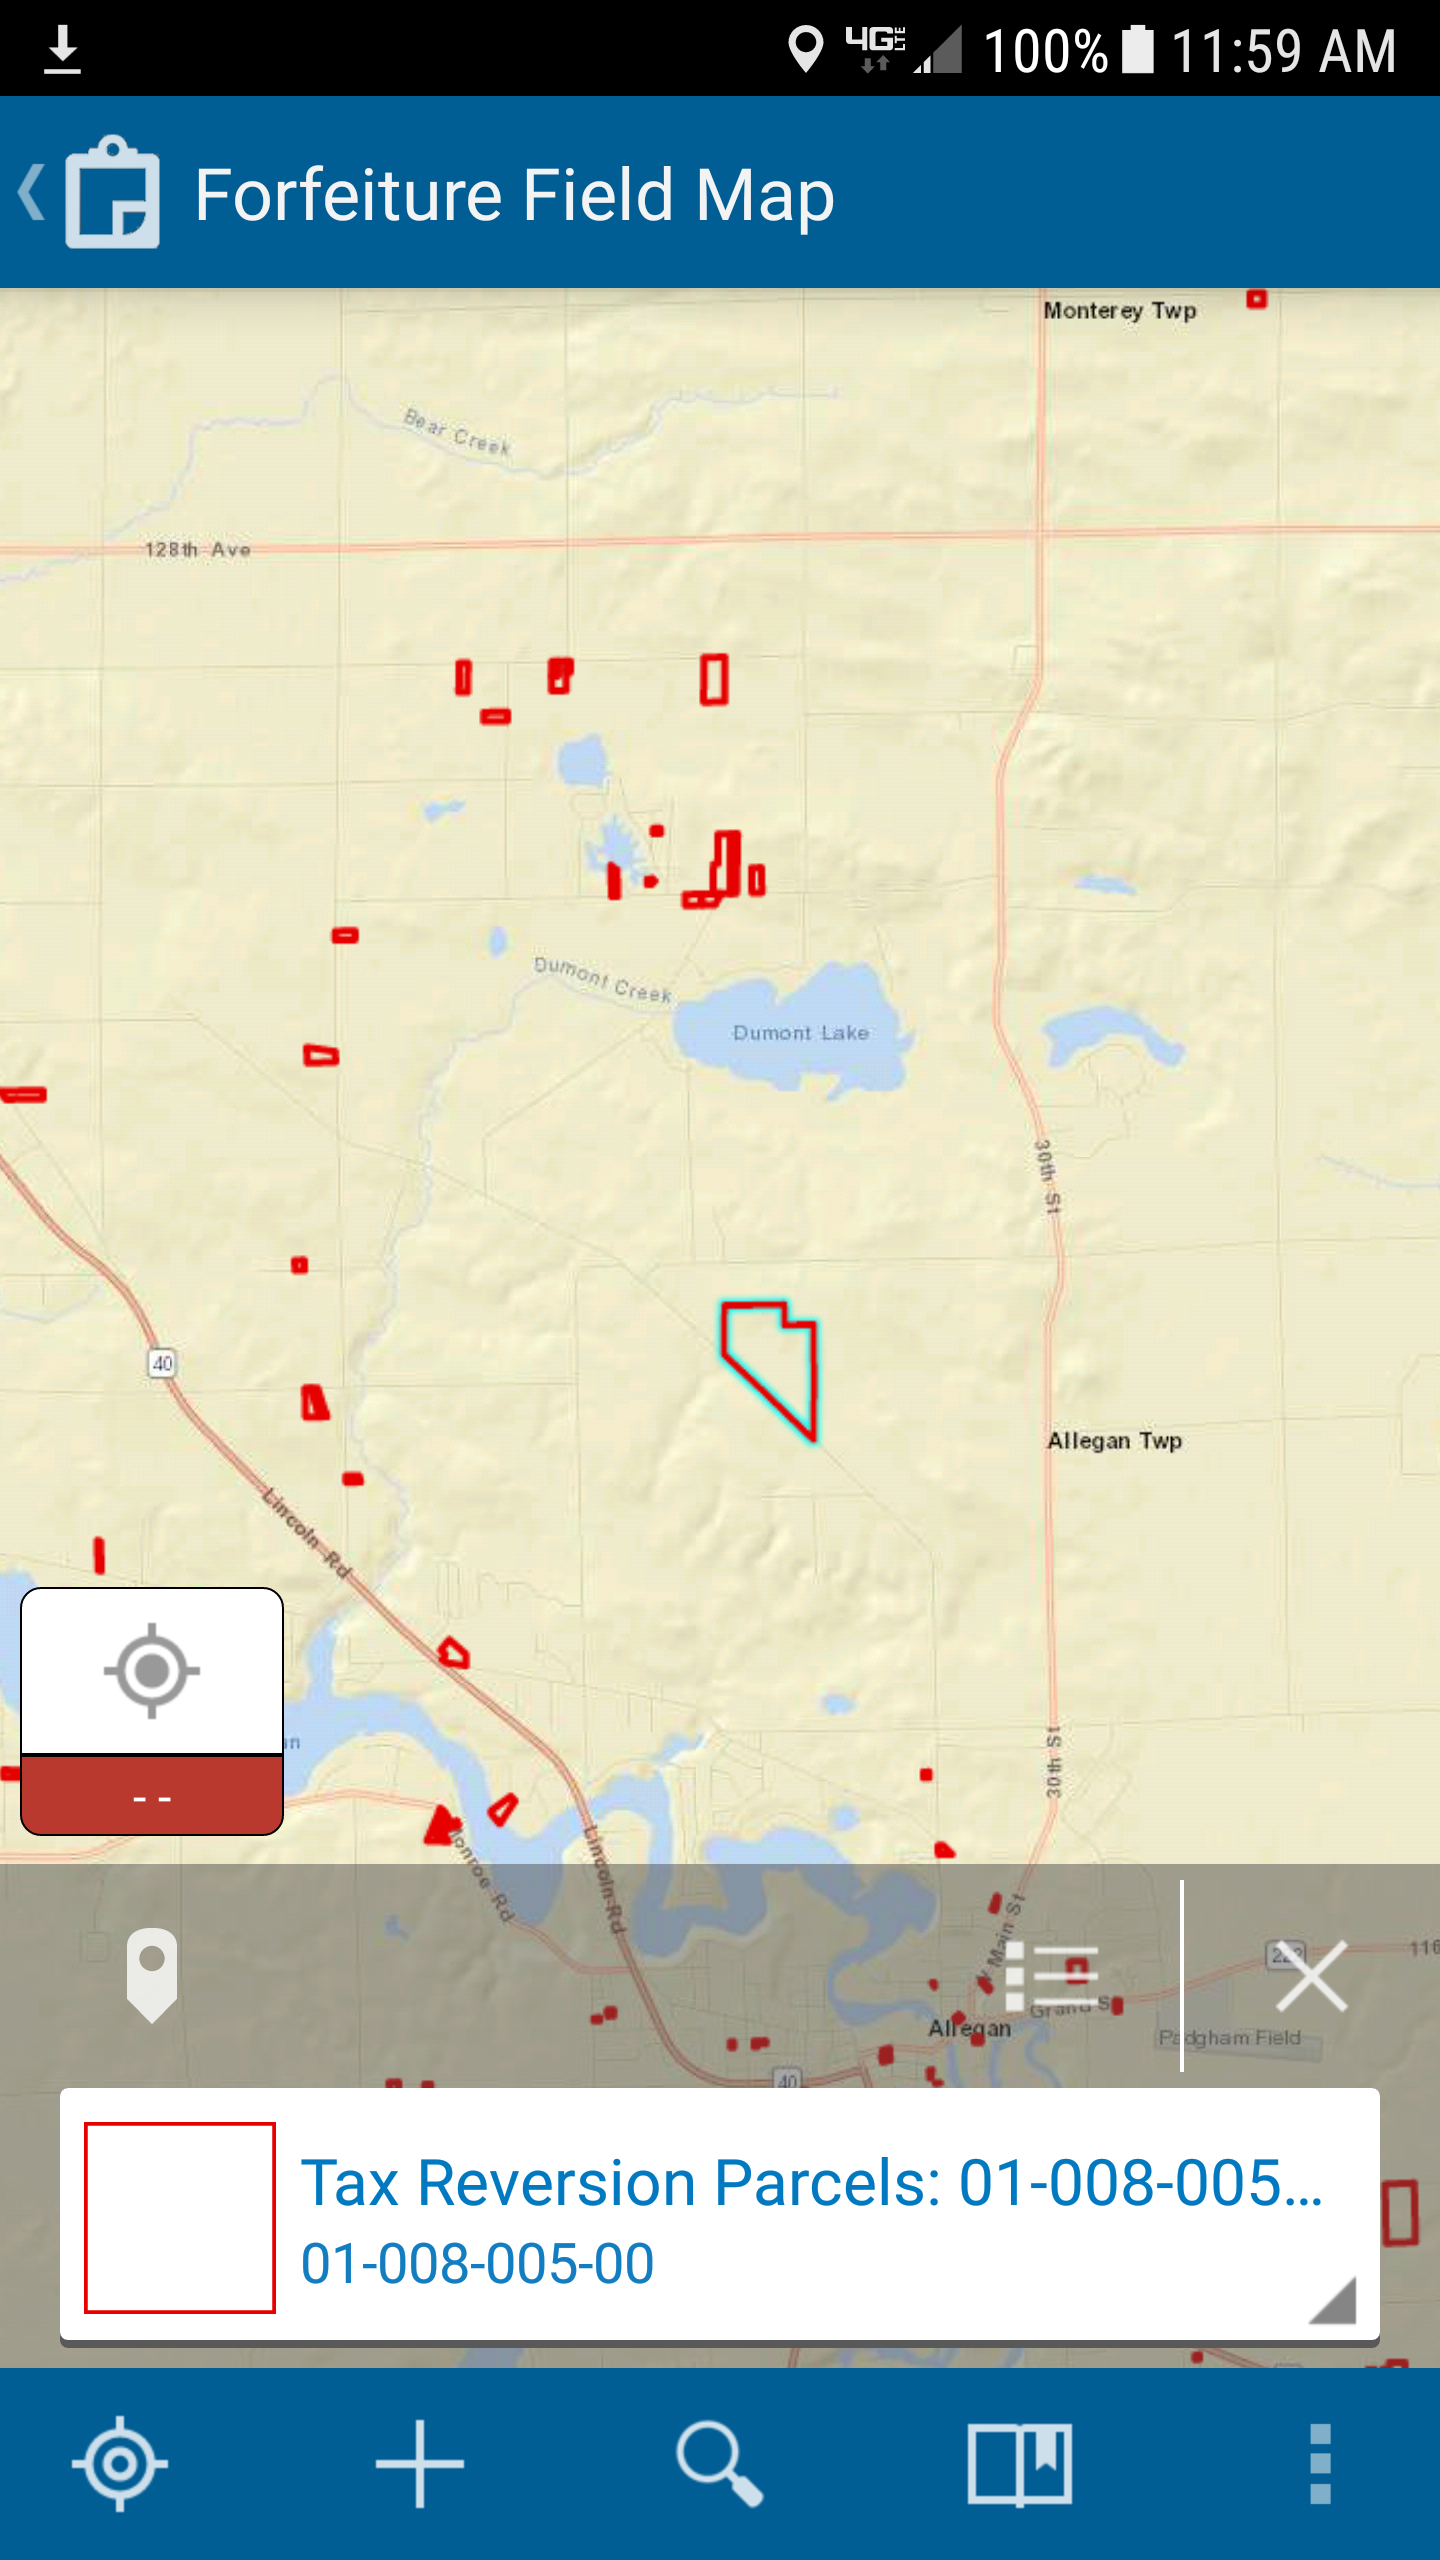
\includegraphics[width=.3\textwidth]{selectParcel.png}
\caption {Select Parcel}
\vspace{.25in}
\HRule \\[.4cm] % Horizontal Line added
\vspace{.25in}
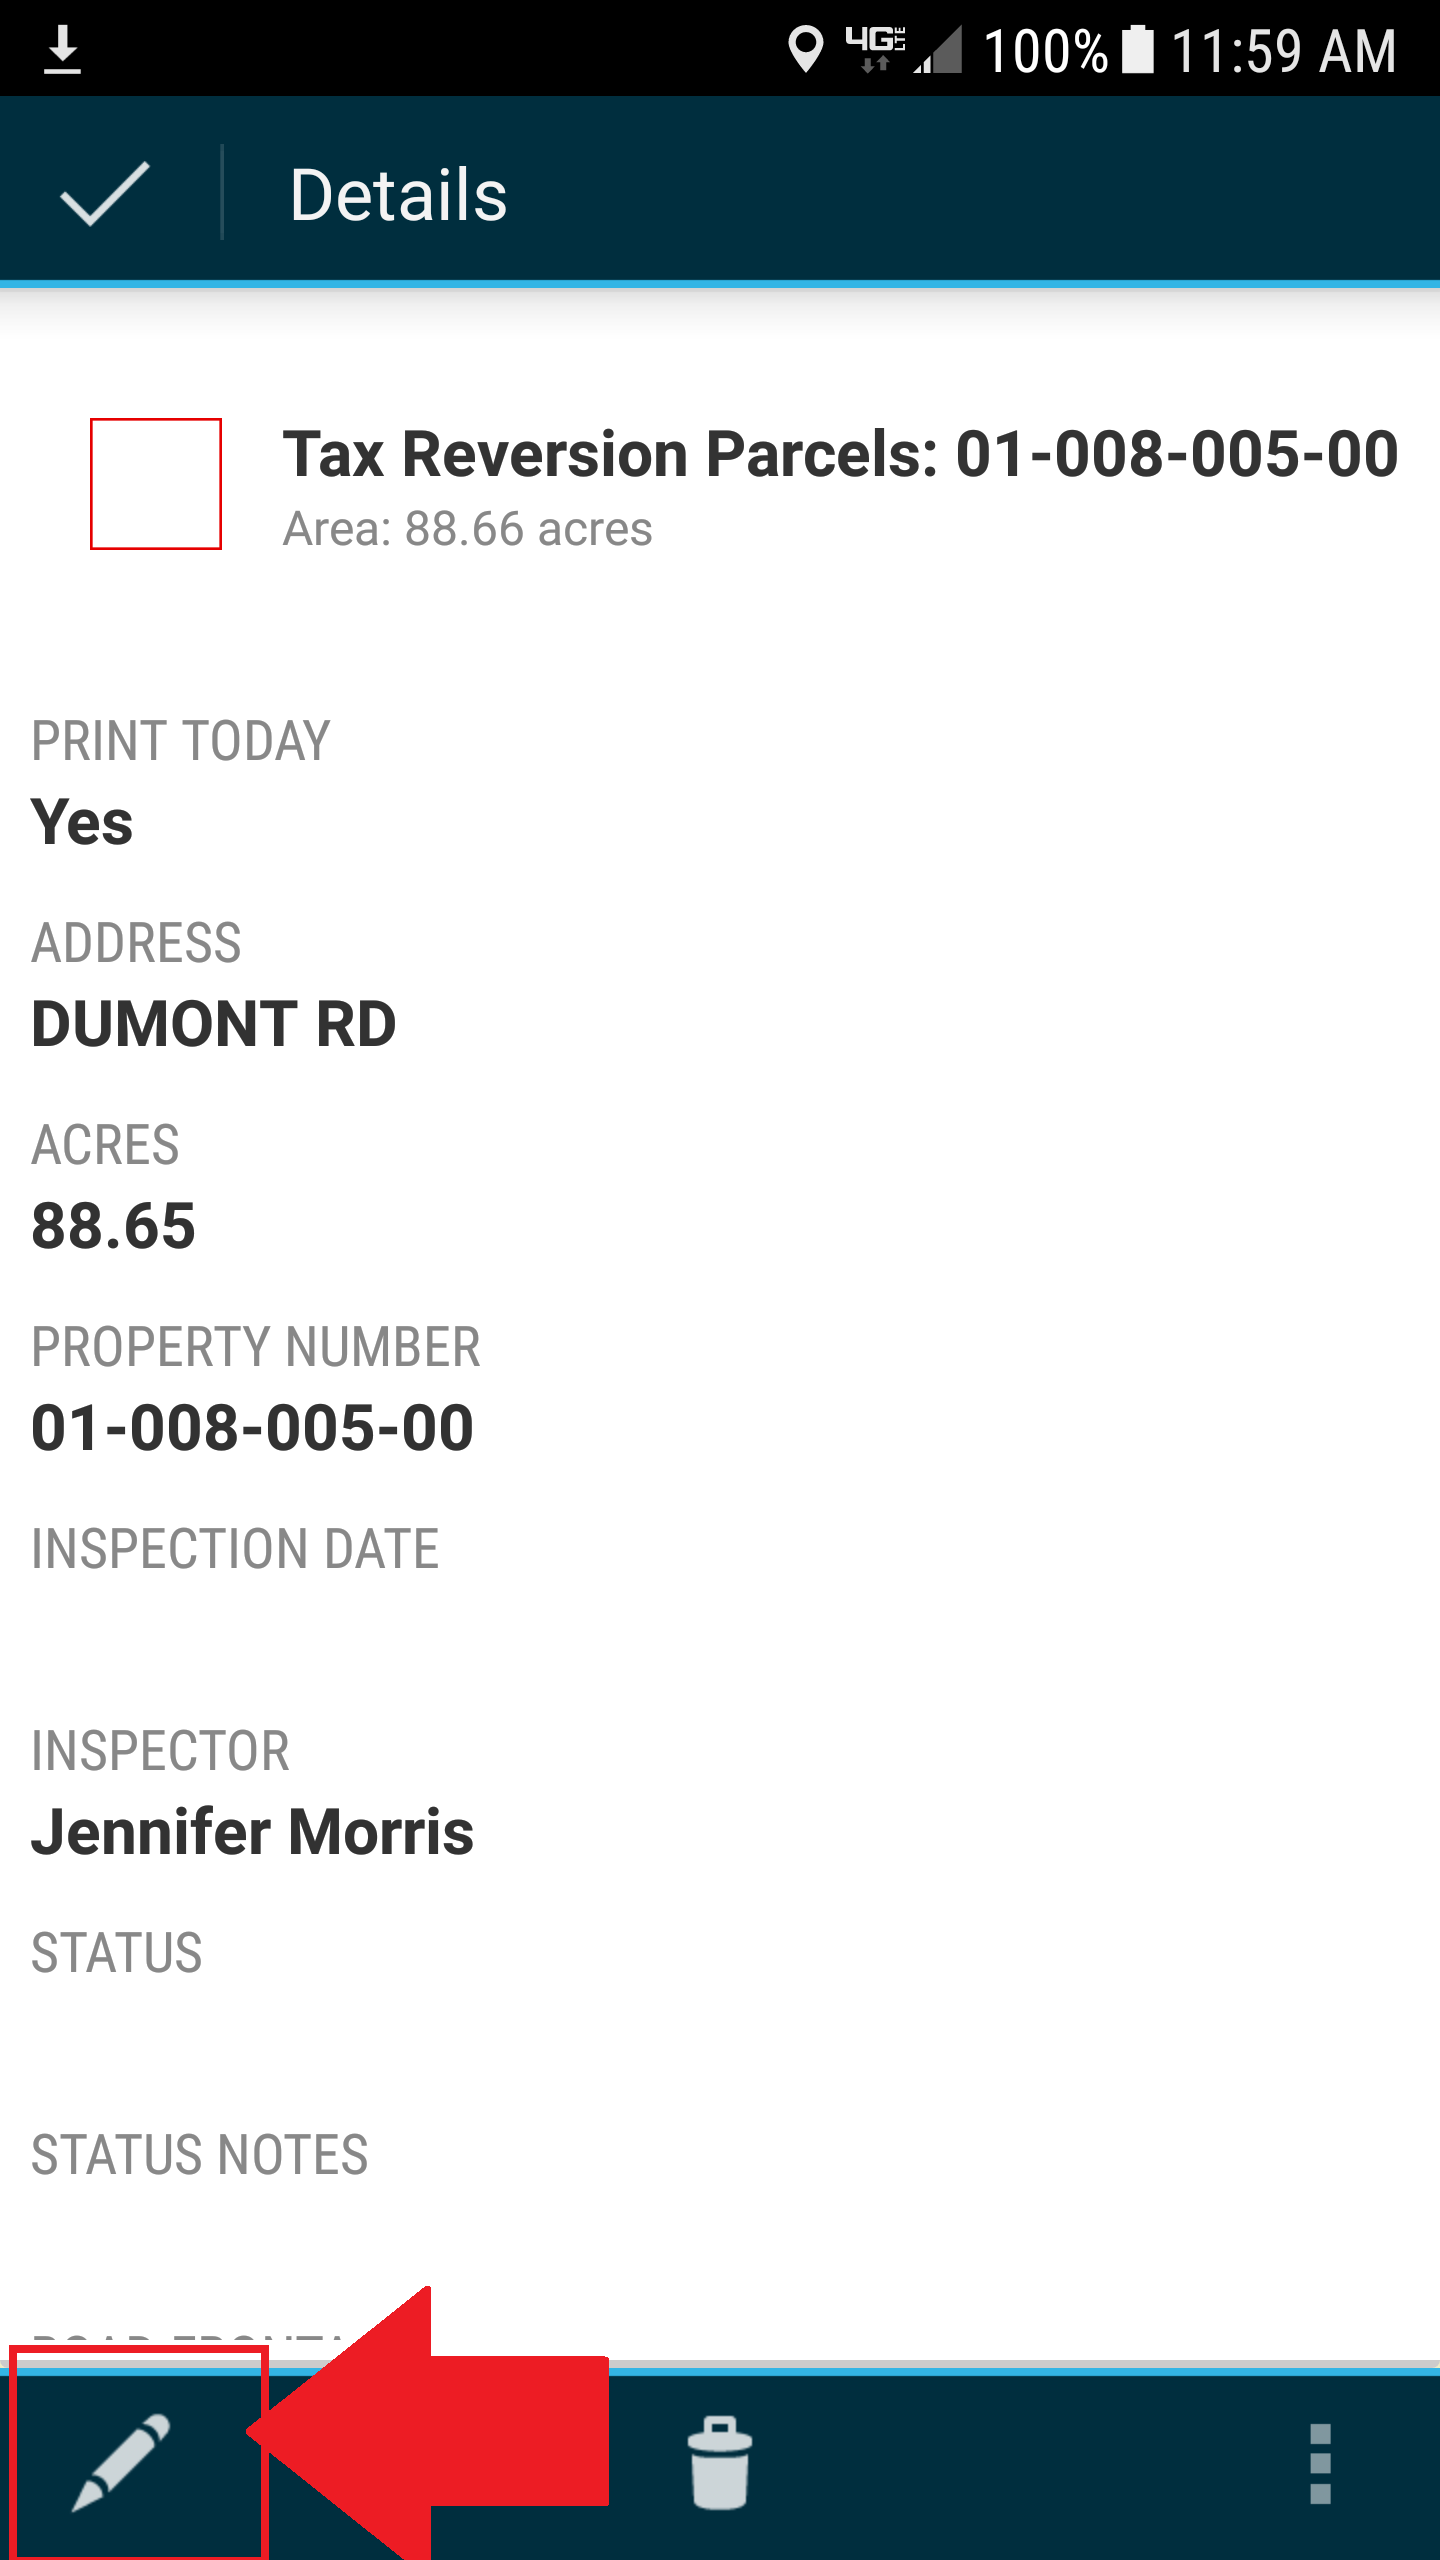
\includegraphics[width=.3\textwidth]{parcelDetails.png}
\caption{Parcel Details}
\end{wrapfigure}
\vspace{1in}
In the Forfeiture Field Map, for each site visited:\\
\vspace{1in}
\textbf{Select the desired parcel}
\vspace{3in}
Push the \Large edit button 
\clearpage
Class prefilled
Acres prefilled
\clearpage
\subparagraph*{Device 1 Field Operation Cont.}
\subparagraph*{\\}
\begin{wrapfigure}{r}{0.5\textwidth}
\centering
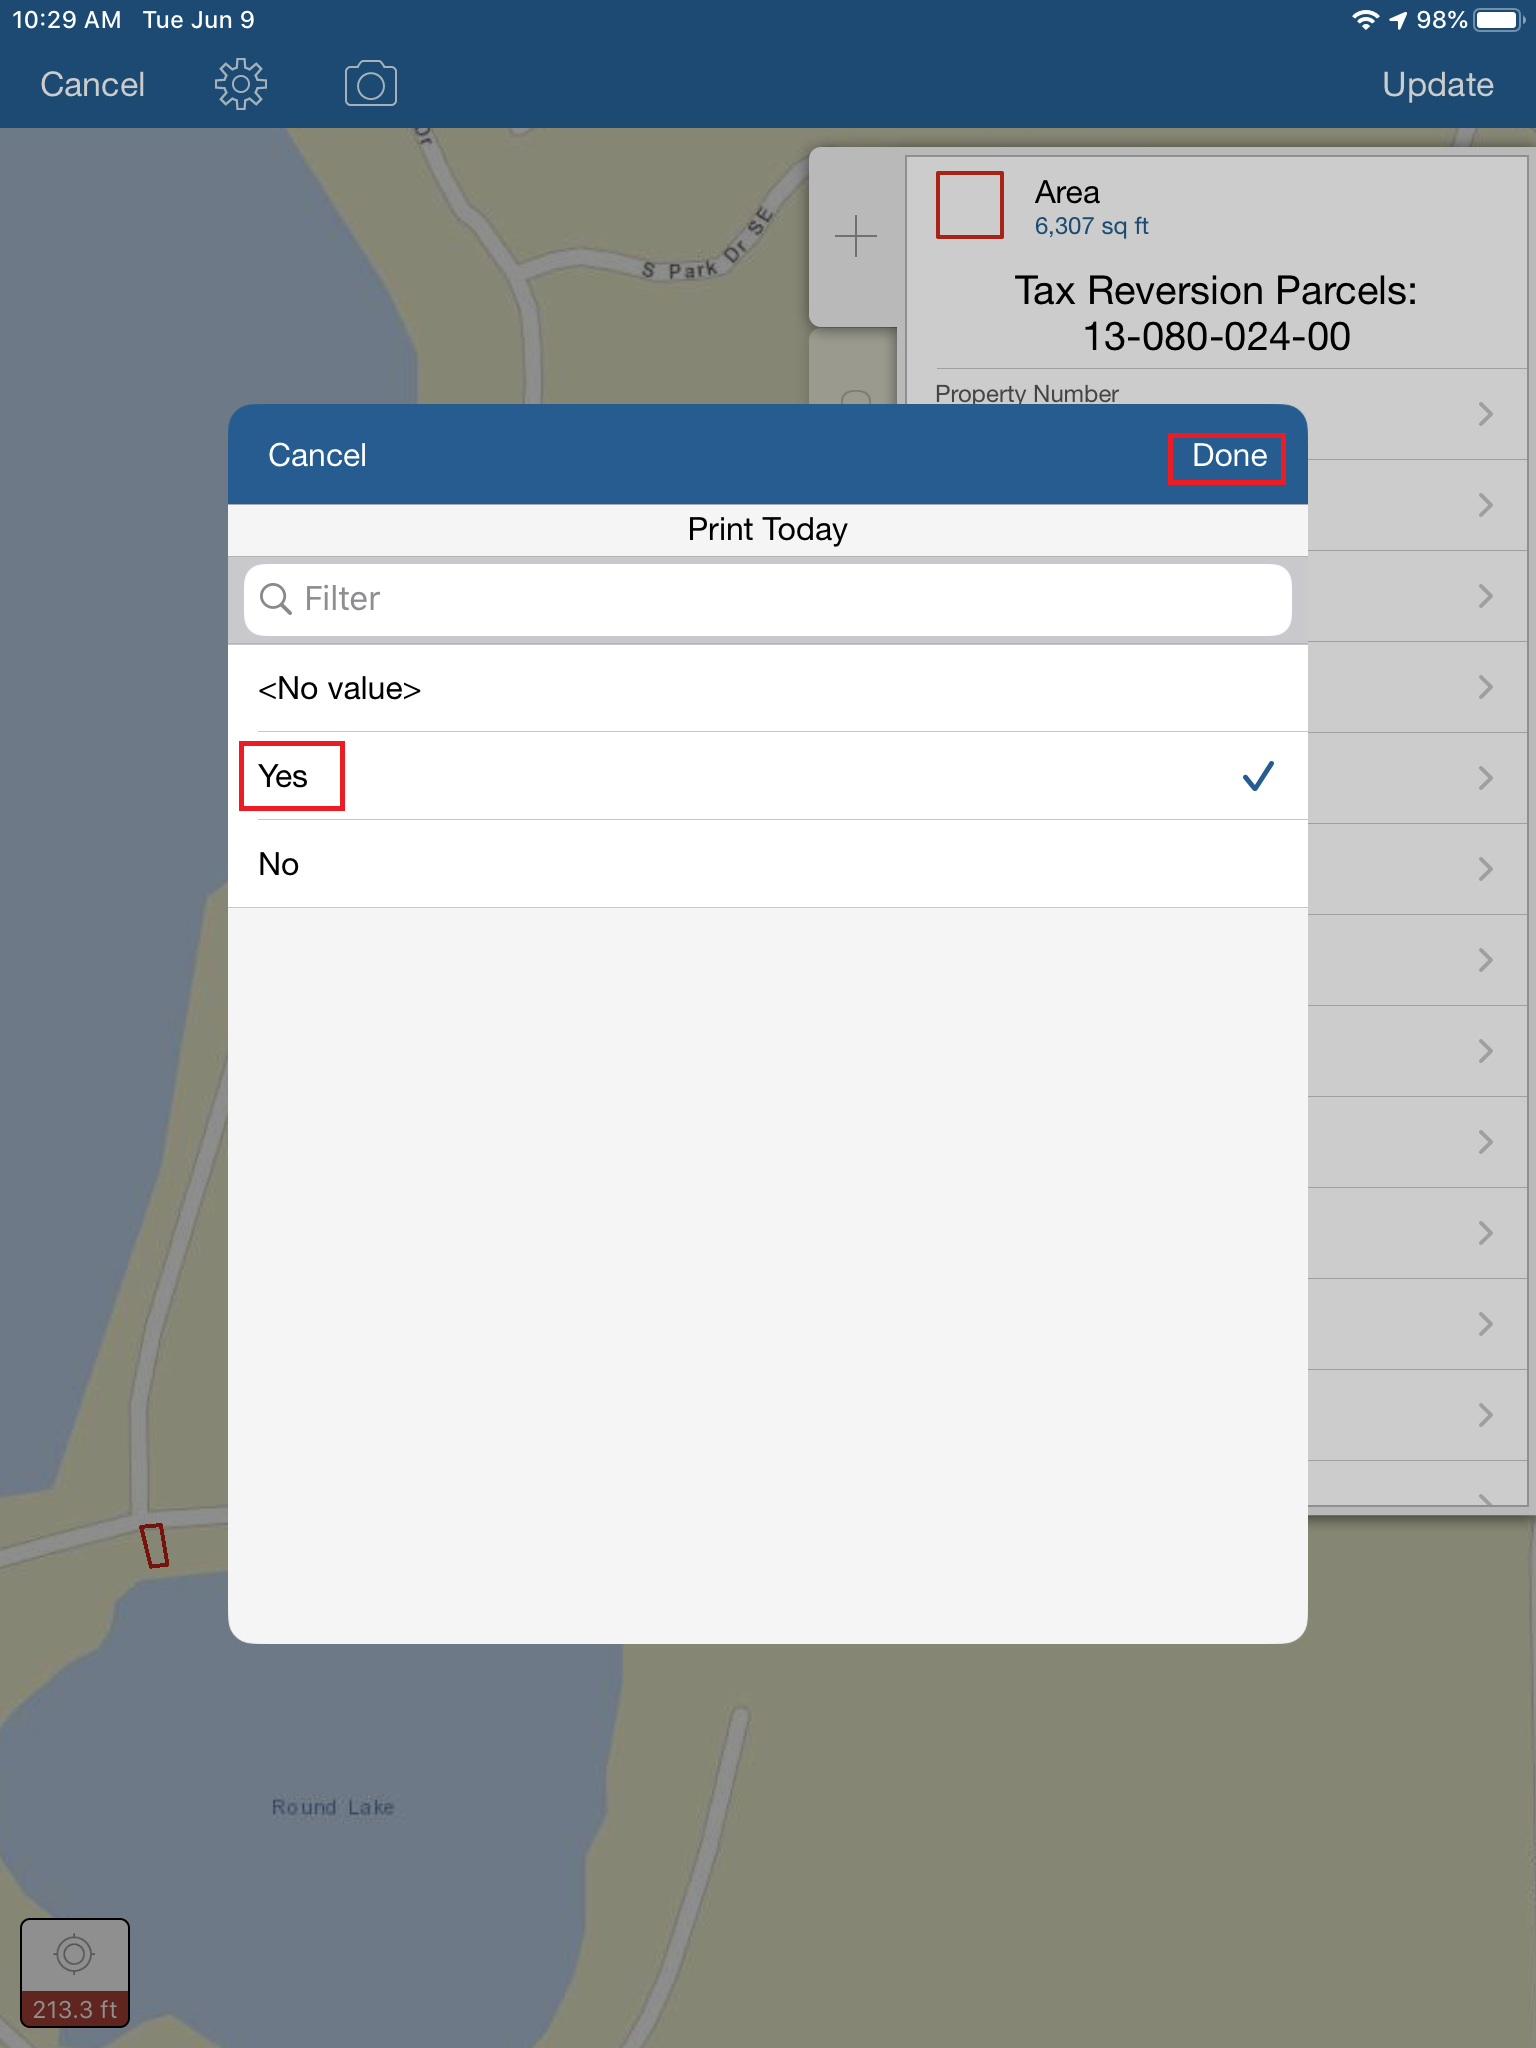
\includegraphics[width=.2\textwidth]{printToday.png}
\caption {Print Today Yes or No}
\vspace{.2in}
\HRule \\[.4cm] % Horizontal Line added
\vspace{.2in}
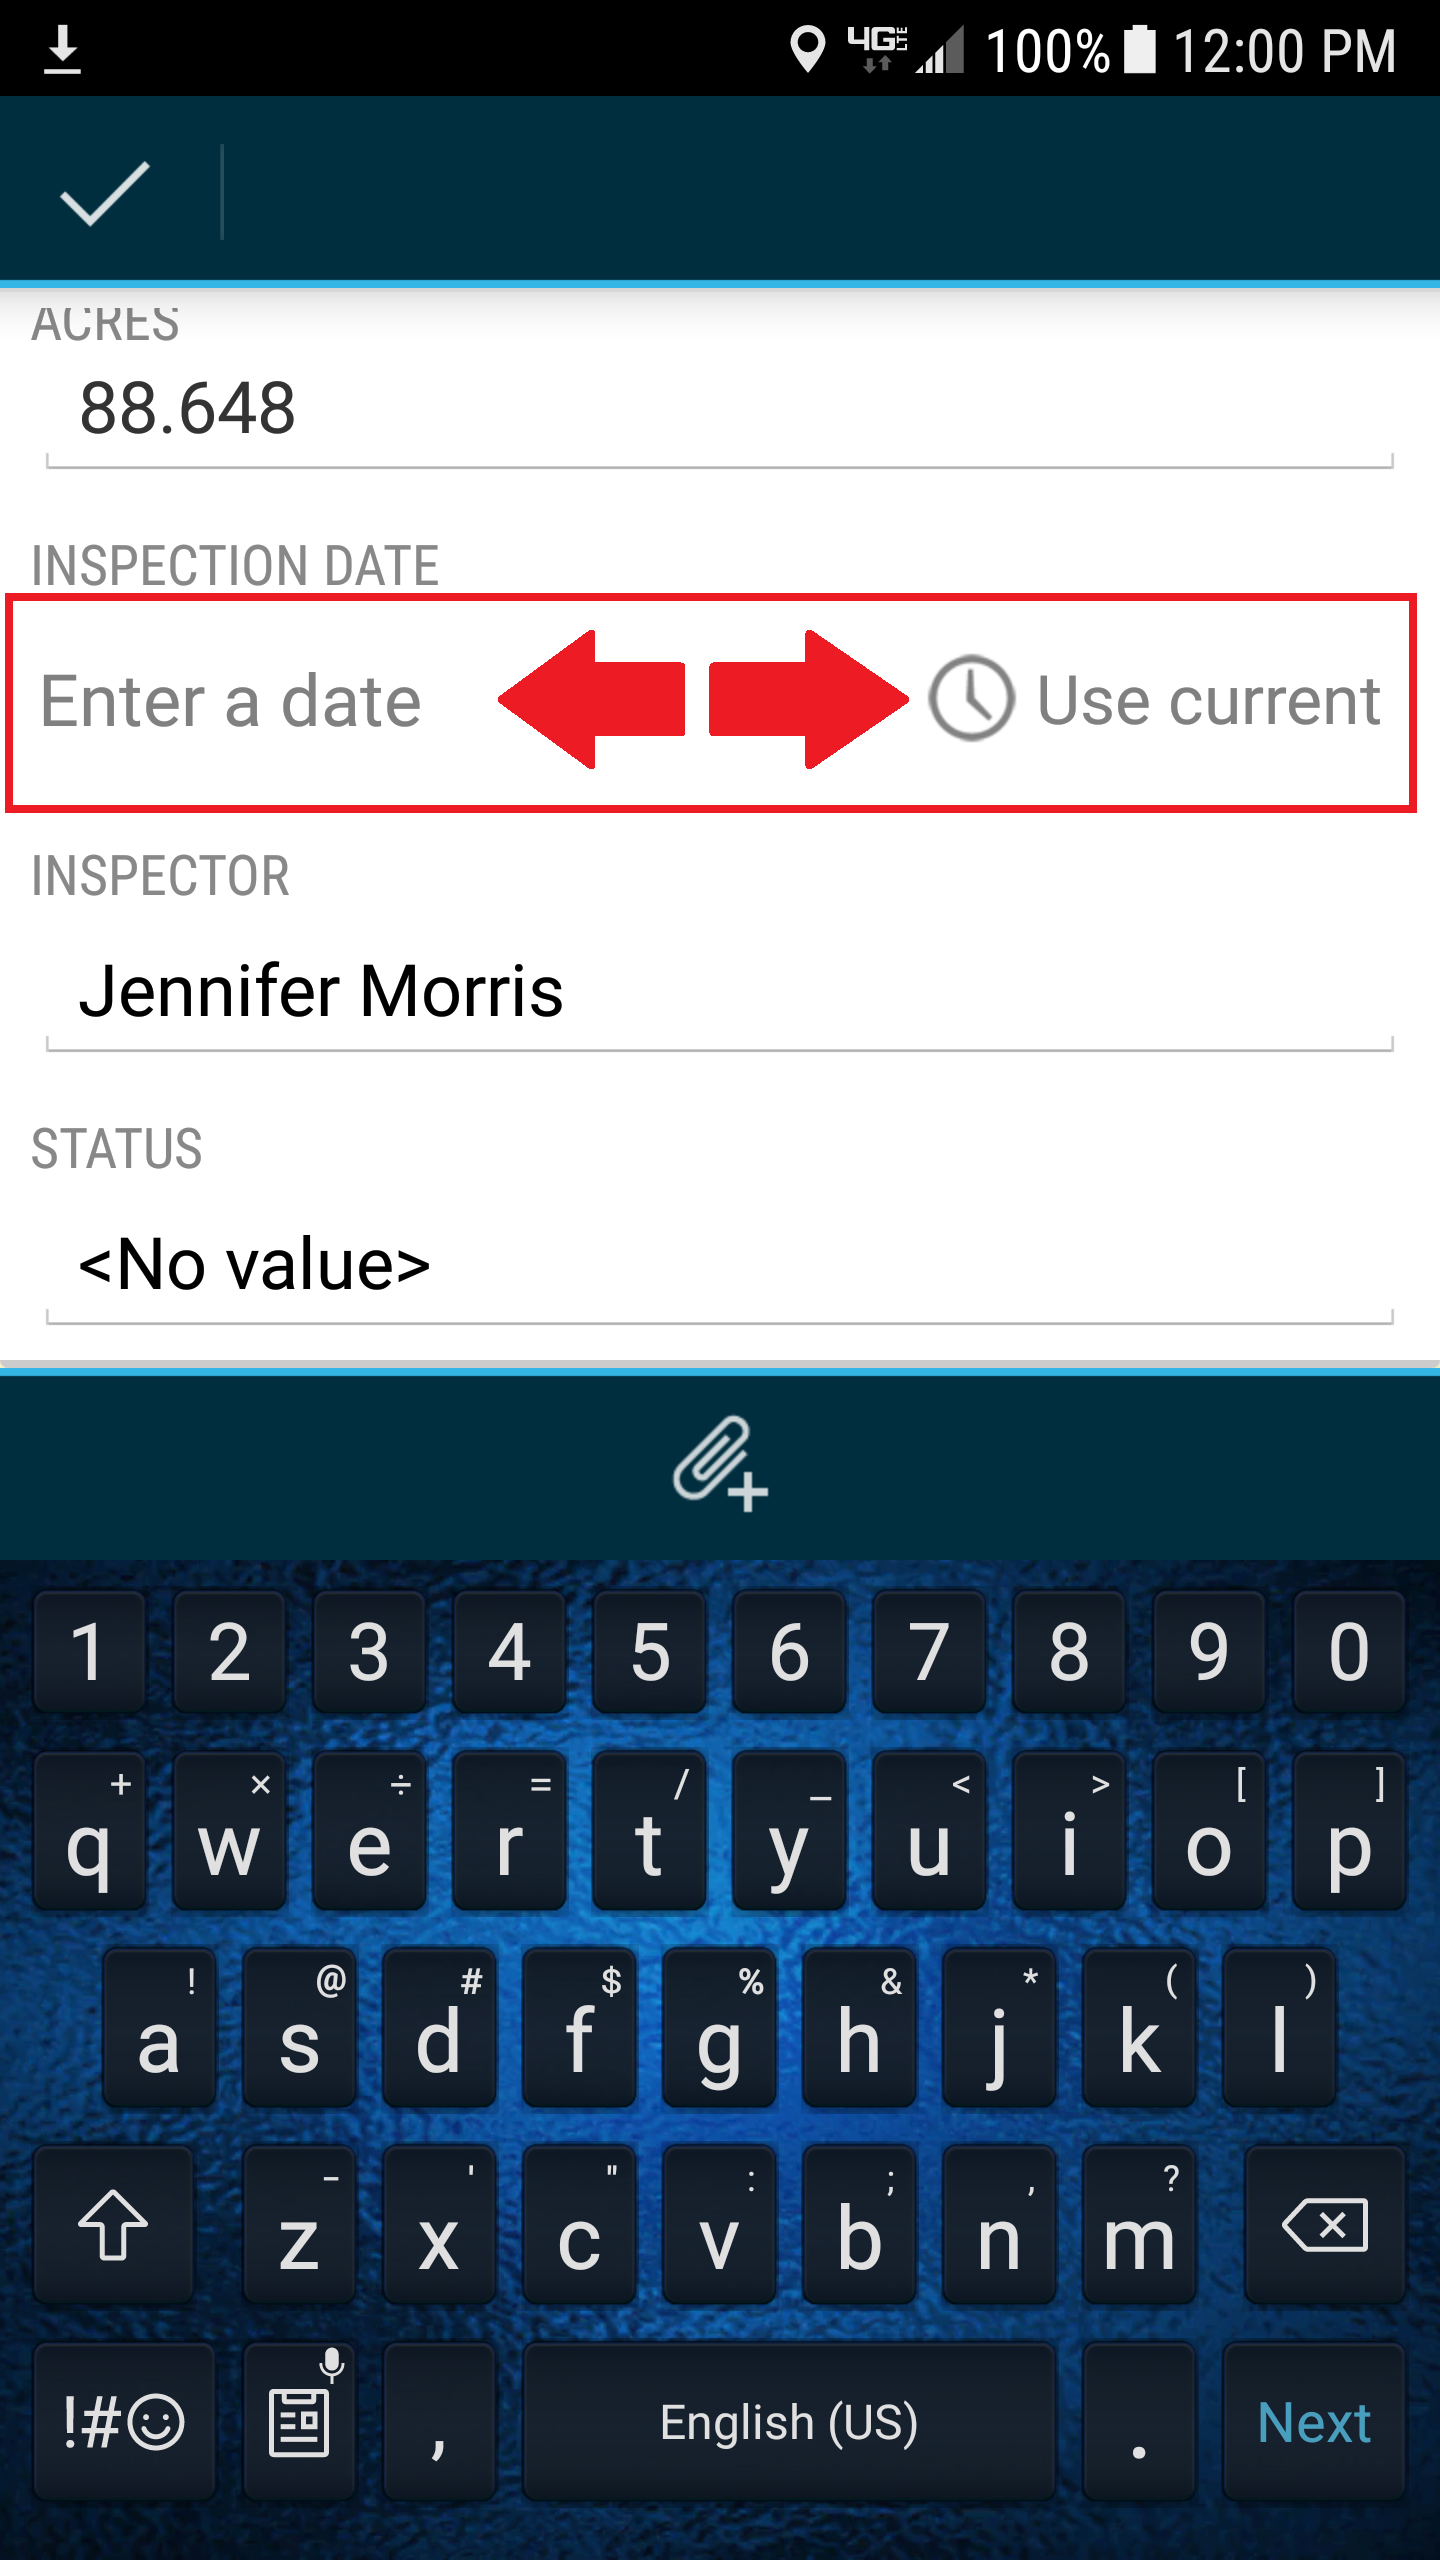
\includegraphics[width=.2\textwidth]{enterDate.png}
\caption{Enter Date}
\vspace{.2in}
\HRule \\[.4cm] % Horizontal Line added
\vspace{.2in}
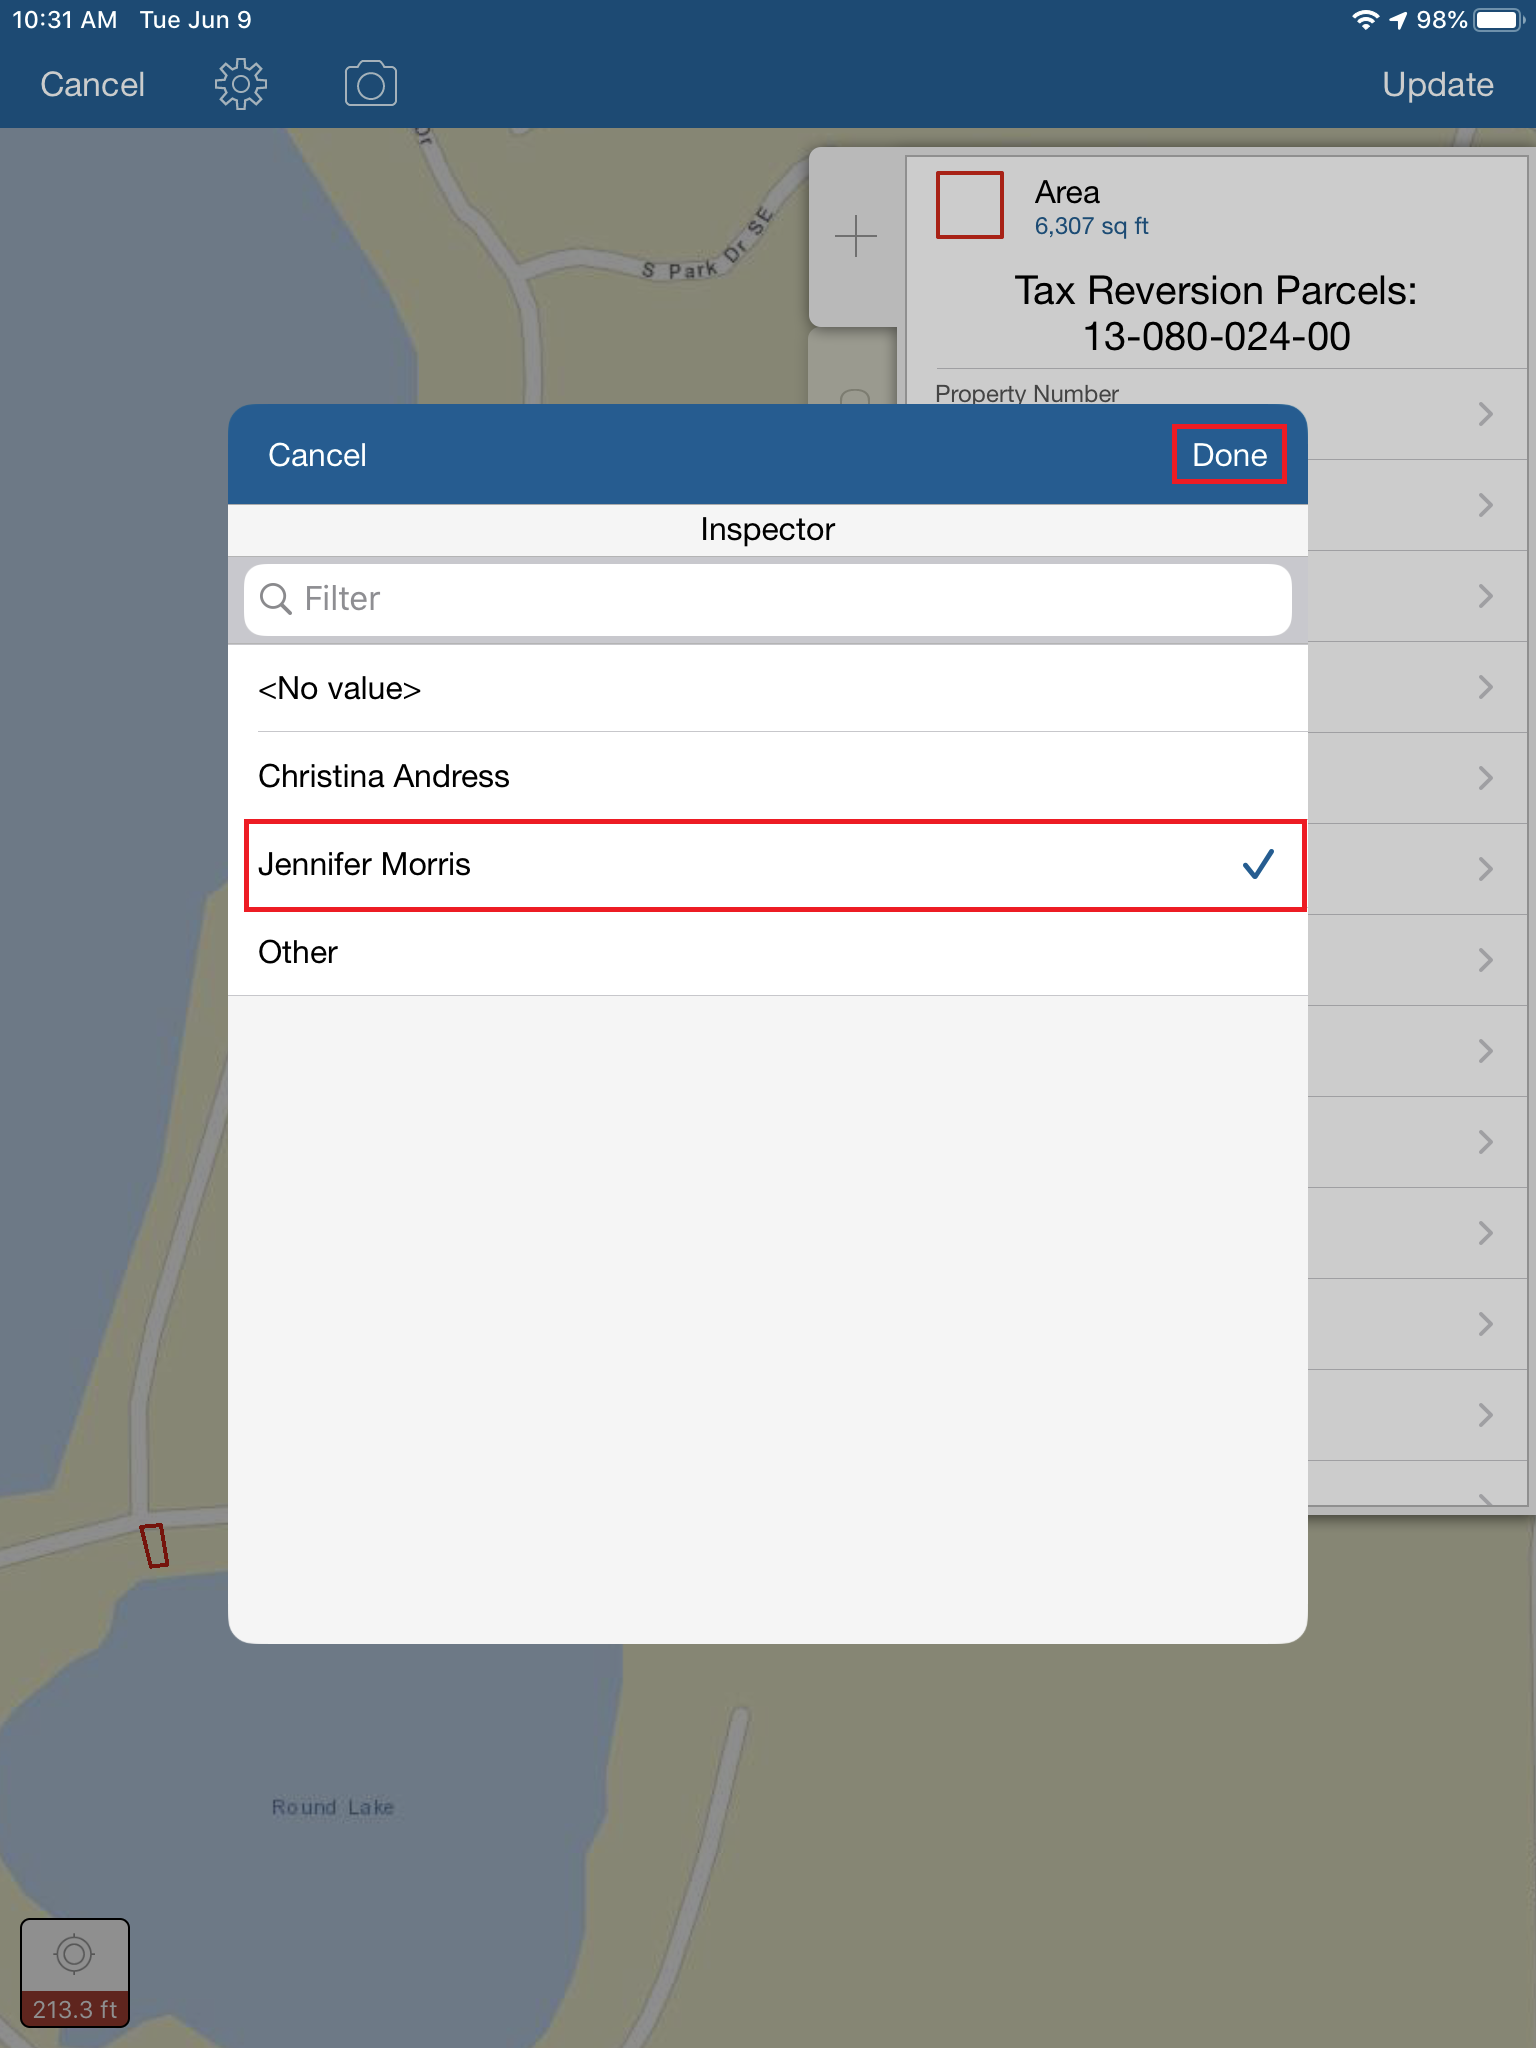
\includegraphics[width=.2\textwidth]{selectInspector.png}
\caption{Select Inspector}
\end{wrapfigure}
Select Yes for Print Today\\
\vspace{2.5in}
\noindent Select Use Current or enter any date\\
\vspace{2in}
\noindent Select Inspector From Dropdown\\
\clearpage
\subparagraph*{Device 1 Field Operation Cont.}
\subparagraph*{\\}
\begin{wrapfigure}{r}{0.5\textwidth}
\centering
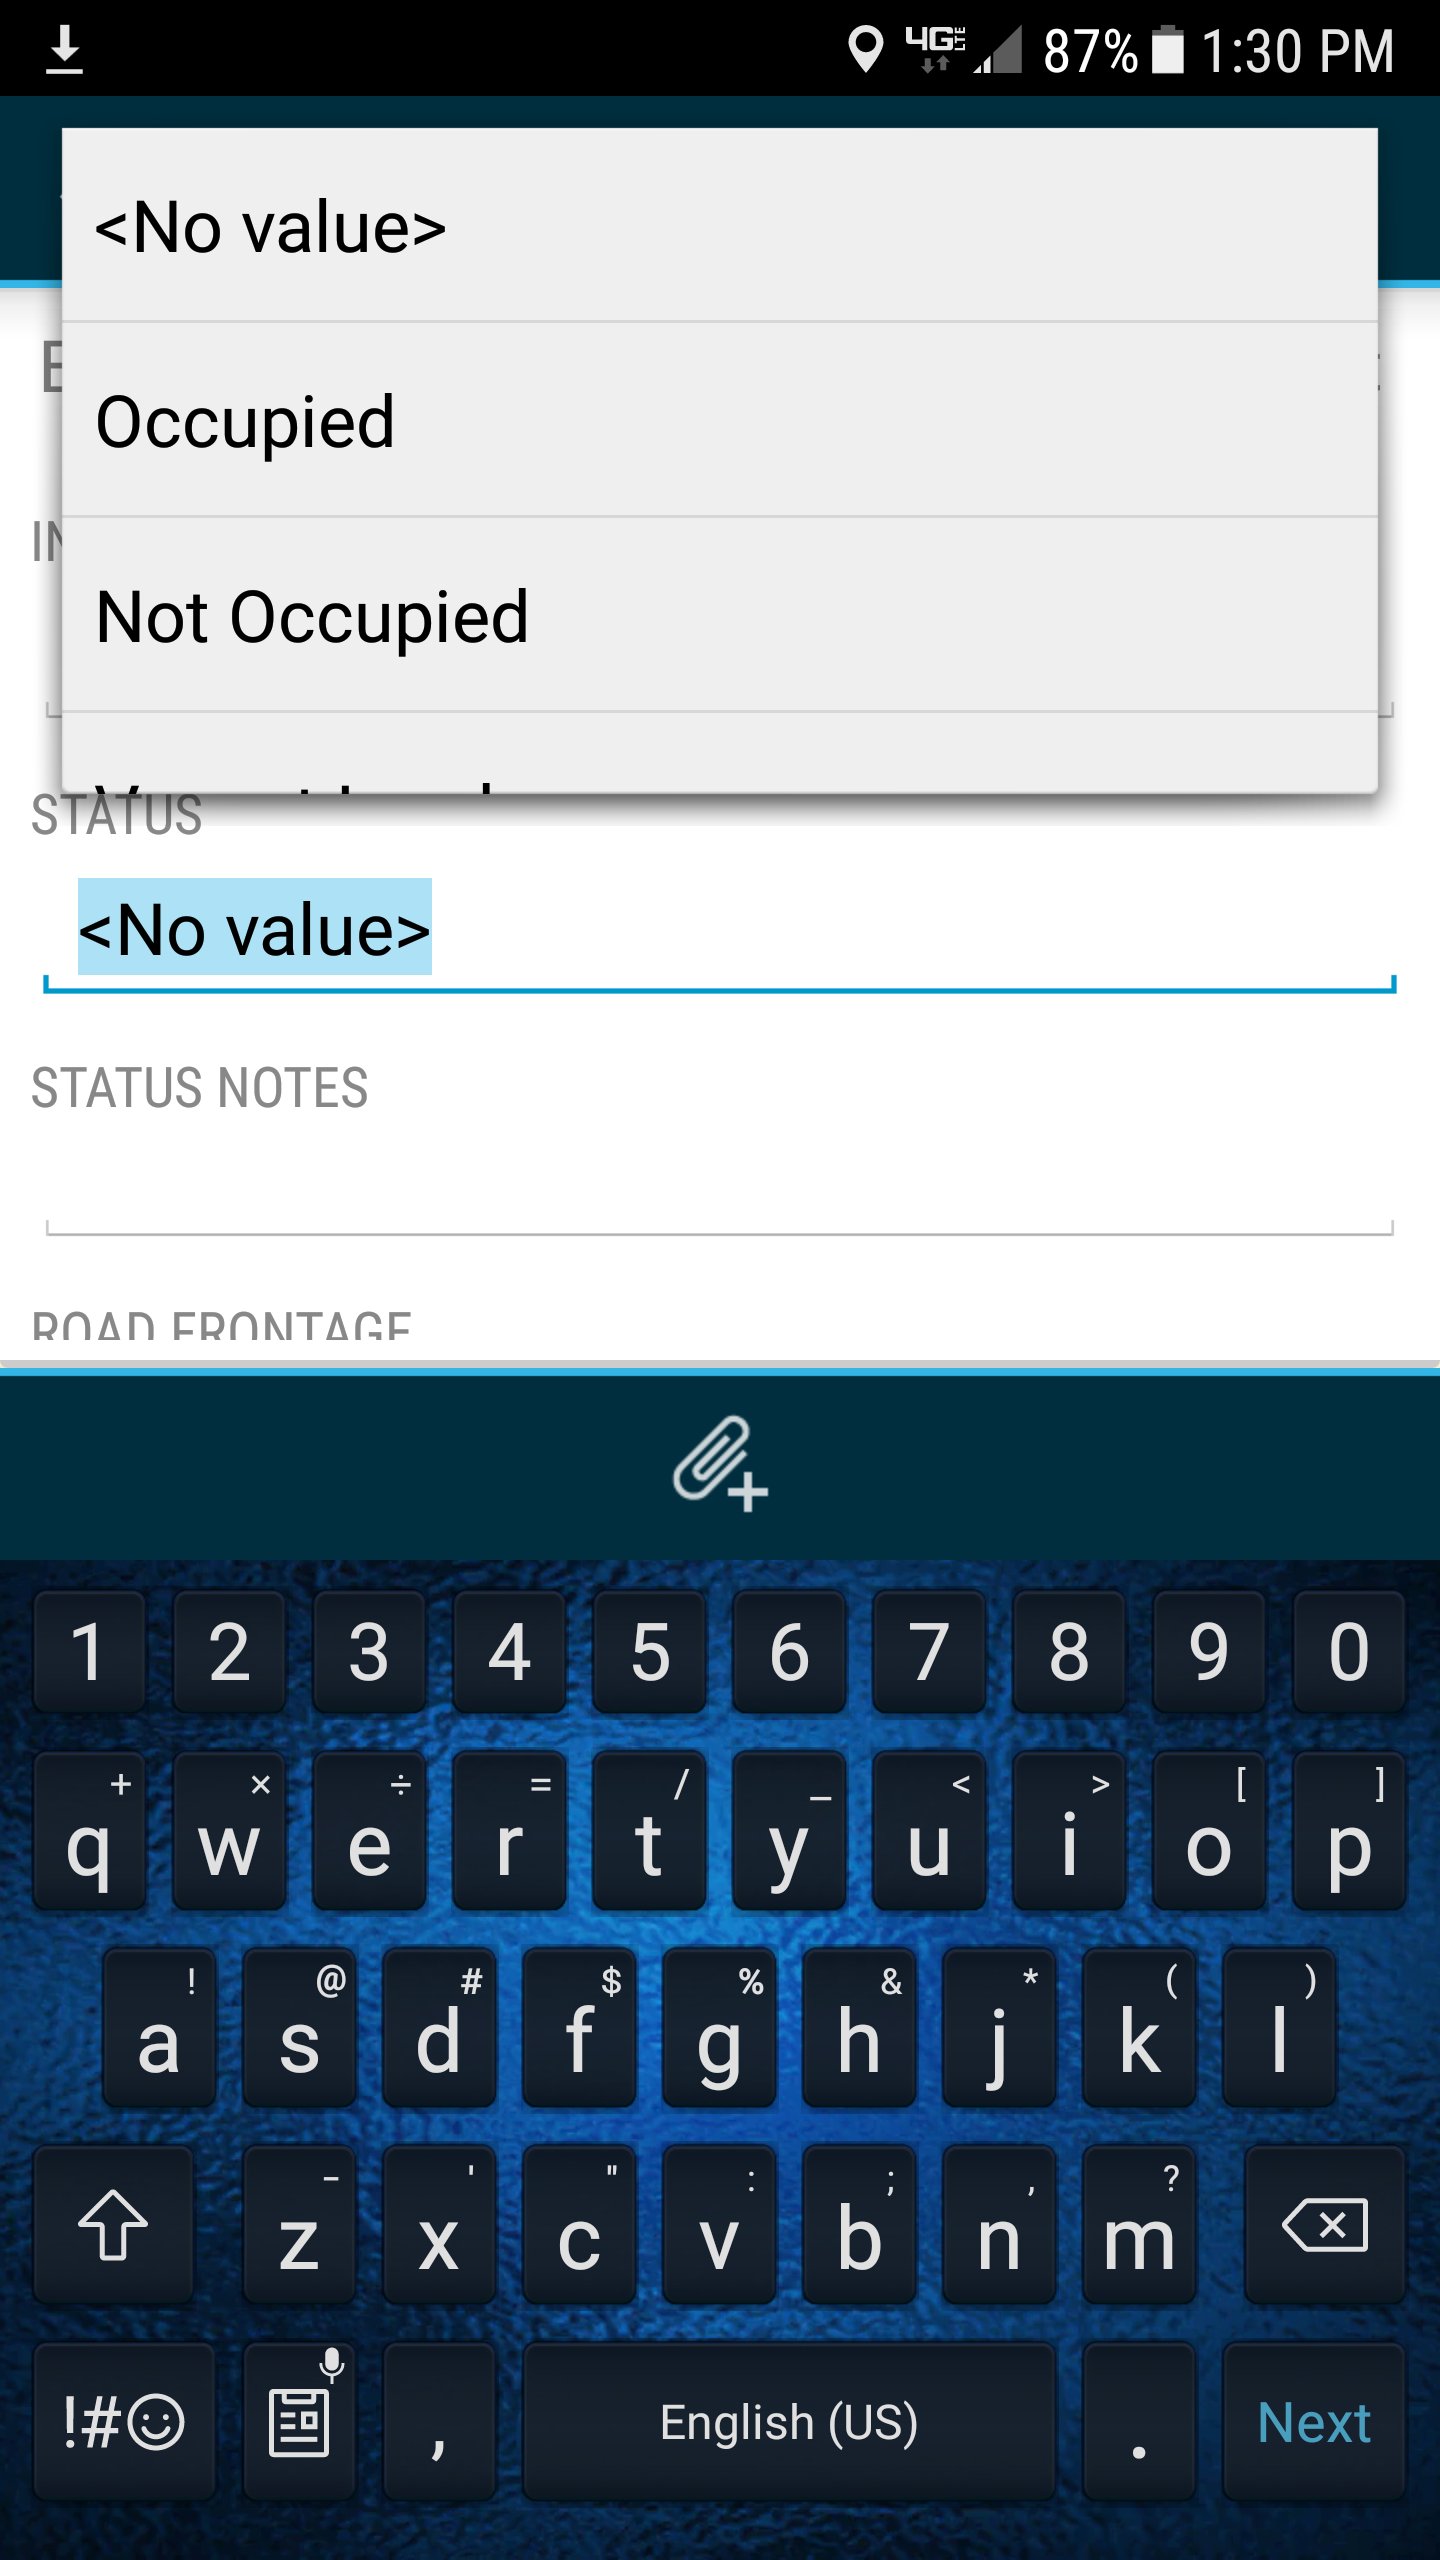
\includegraphics[width=.2\textwidth]{status.png}
\caption {Status}
\vspace{.2in}
\HRule \\[.4cm] % Horizontal Line added
\vspace{.2in}
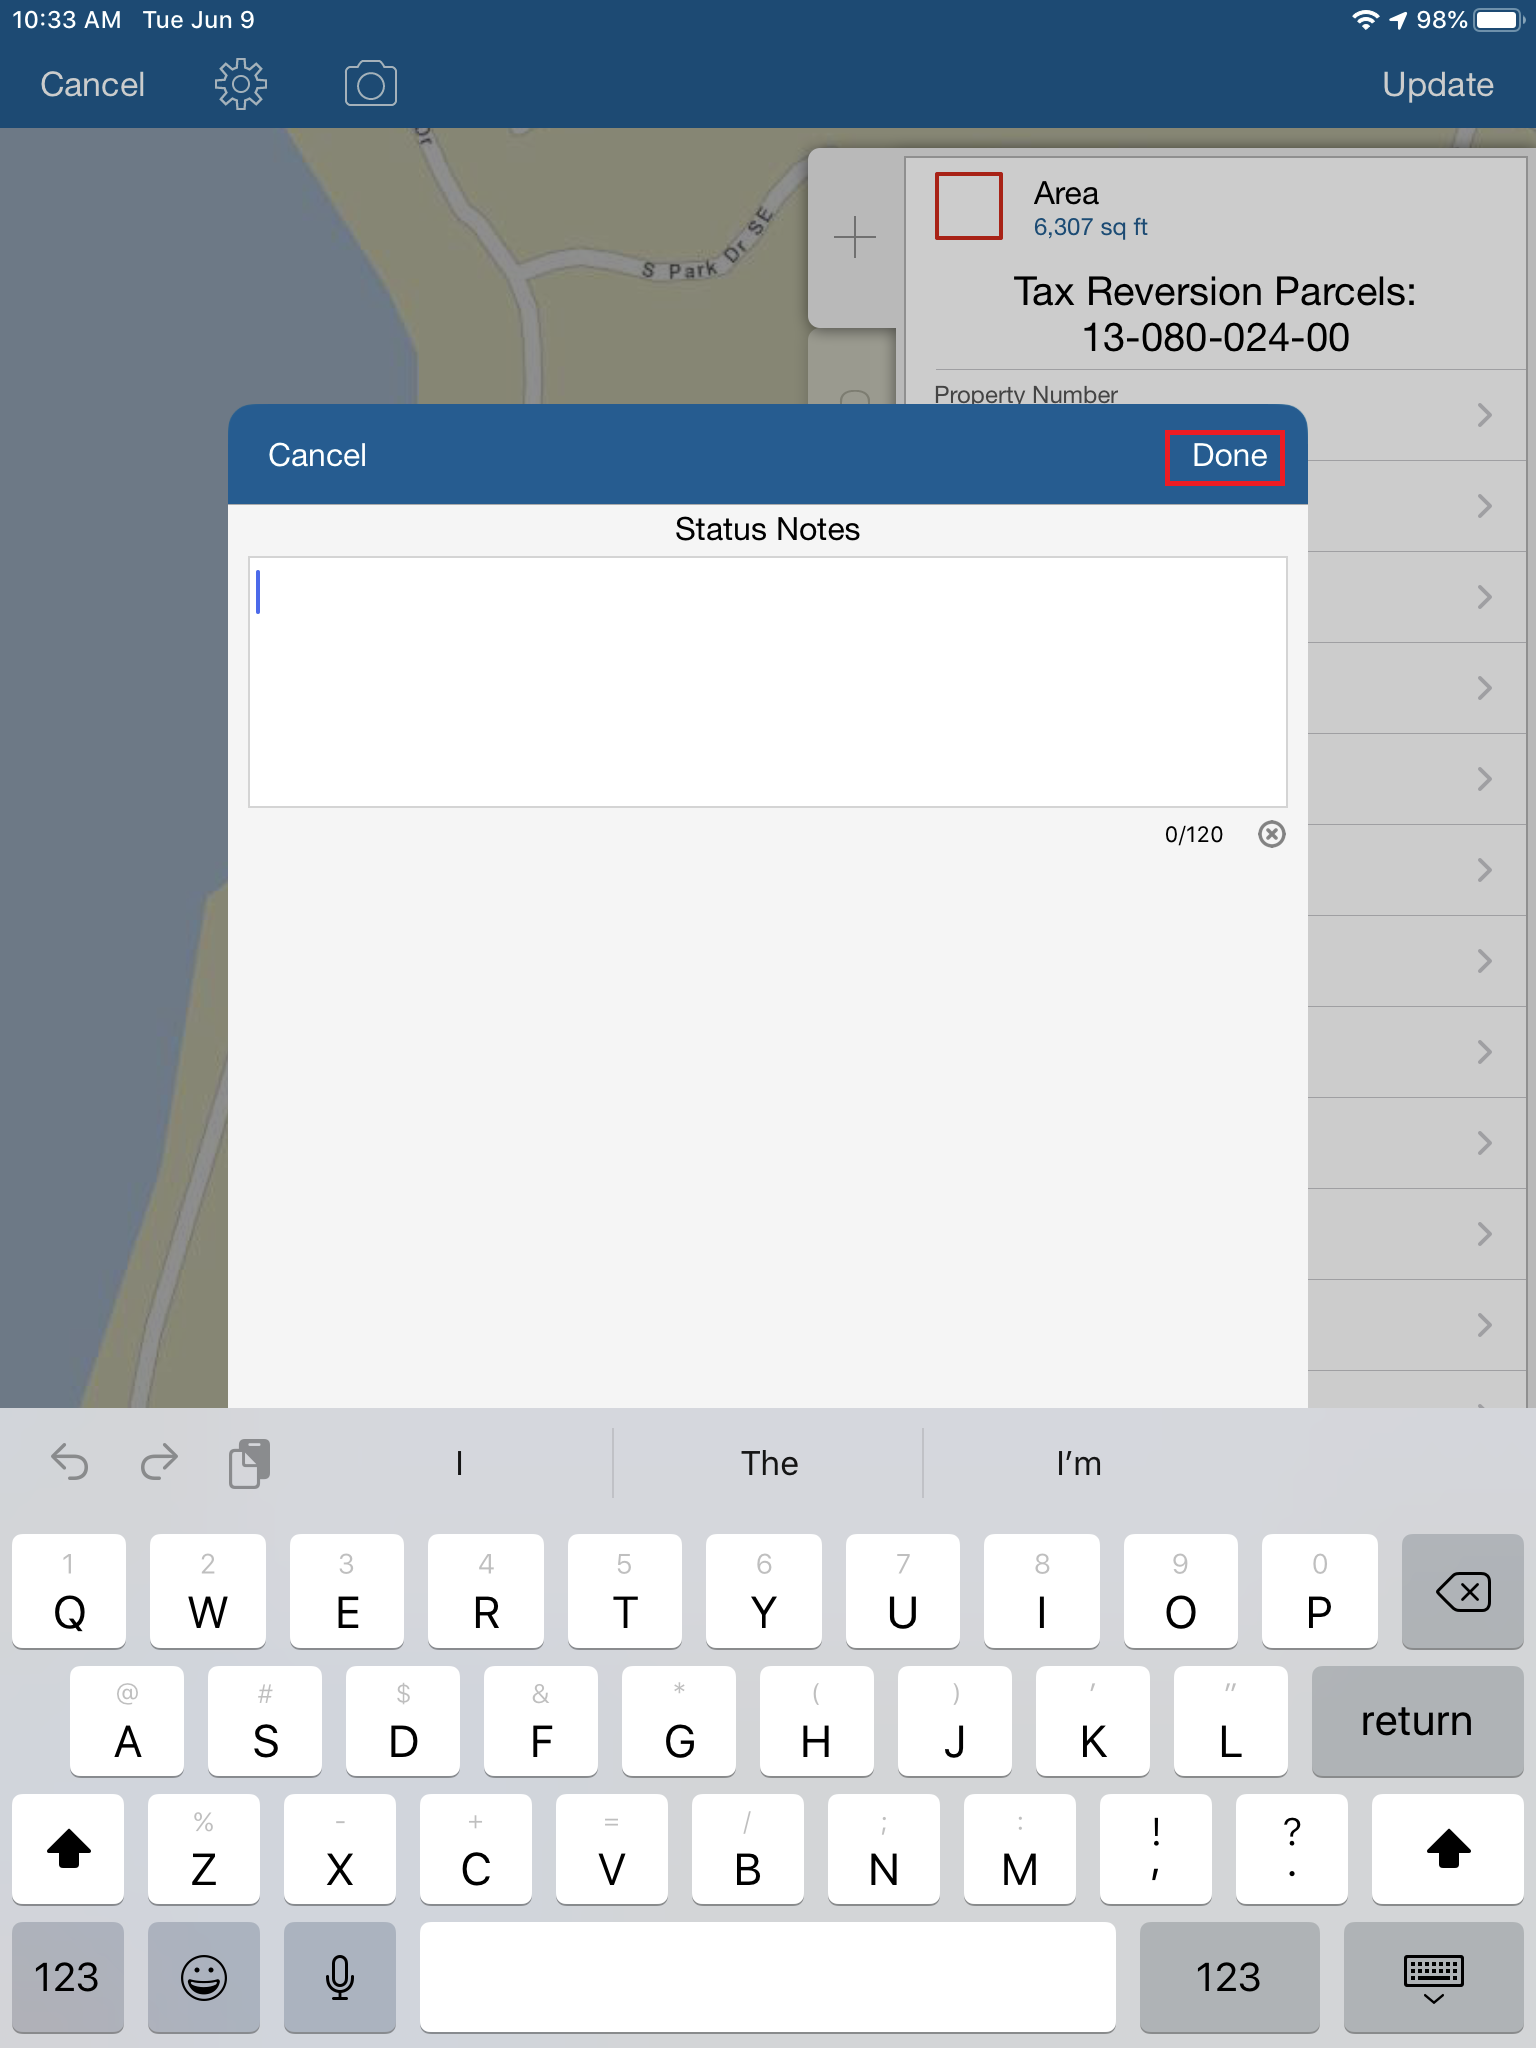
\includegraphics[width=.2\textwidth]{statusNotes.png}
\caption{Status Notes}
\vspace{.2in}
\HRule \\[.4cm] % Horizontal Line added
\vspace{.2in}
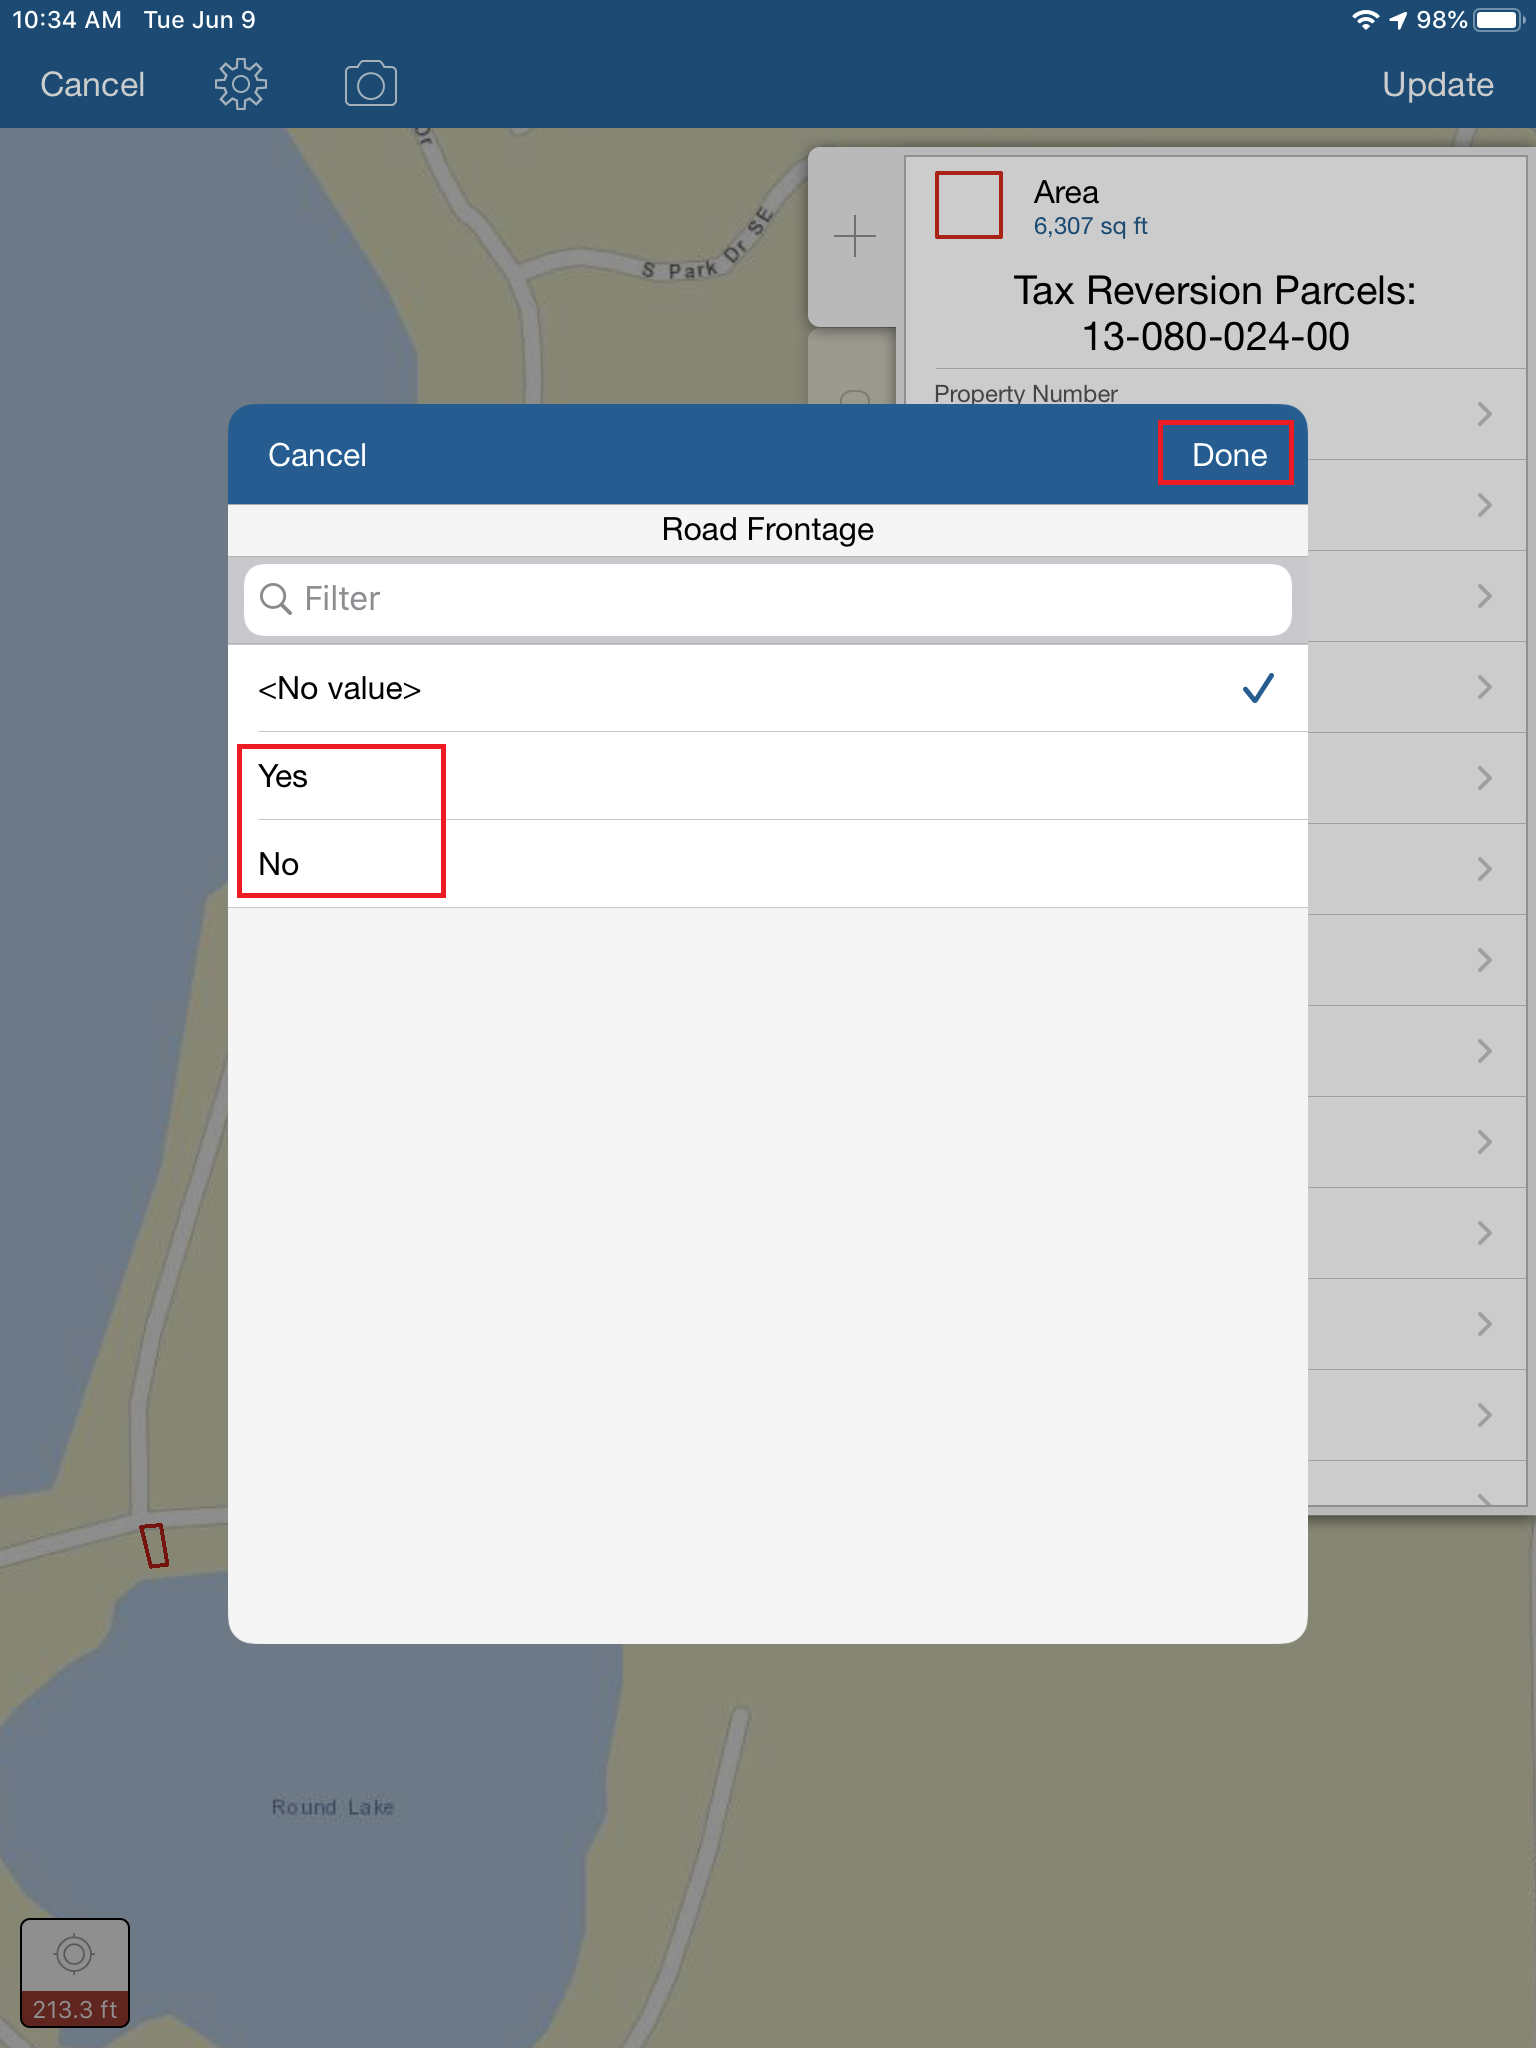
\includegraphics[width=.2\textwidth]{roadFrontage.png}
\caption{Road Frontage}
\end{wrapfigure}
Select Occupied or Not Occupied\\
\vspace{2in}
\noindent Enter status notes up to 120 characters\\
\vspace{2in}
\noindent Select Yes or No for Road Frontage\\
\clearpage
\subparagraph*{Device 1 Field Operation Cont.}
%\subparagraph*{\\}
\begin{wrapfigure}{r}{0.5\textwidth}
\centering
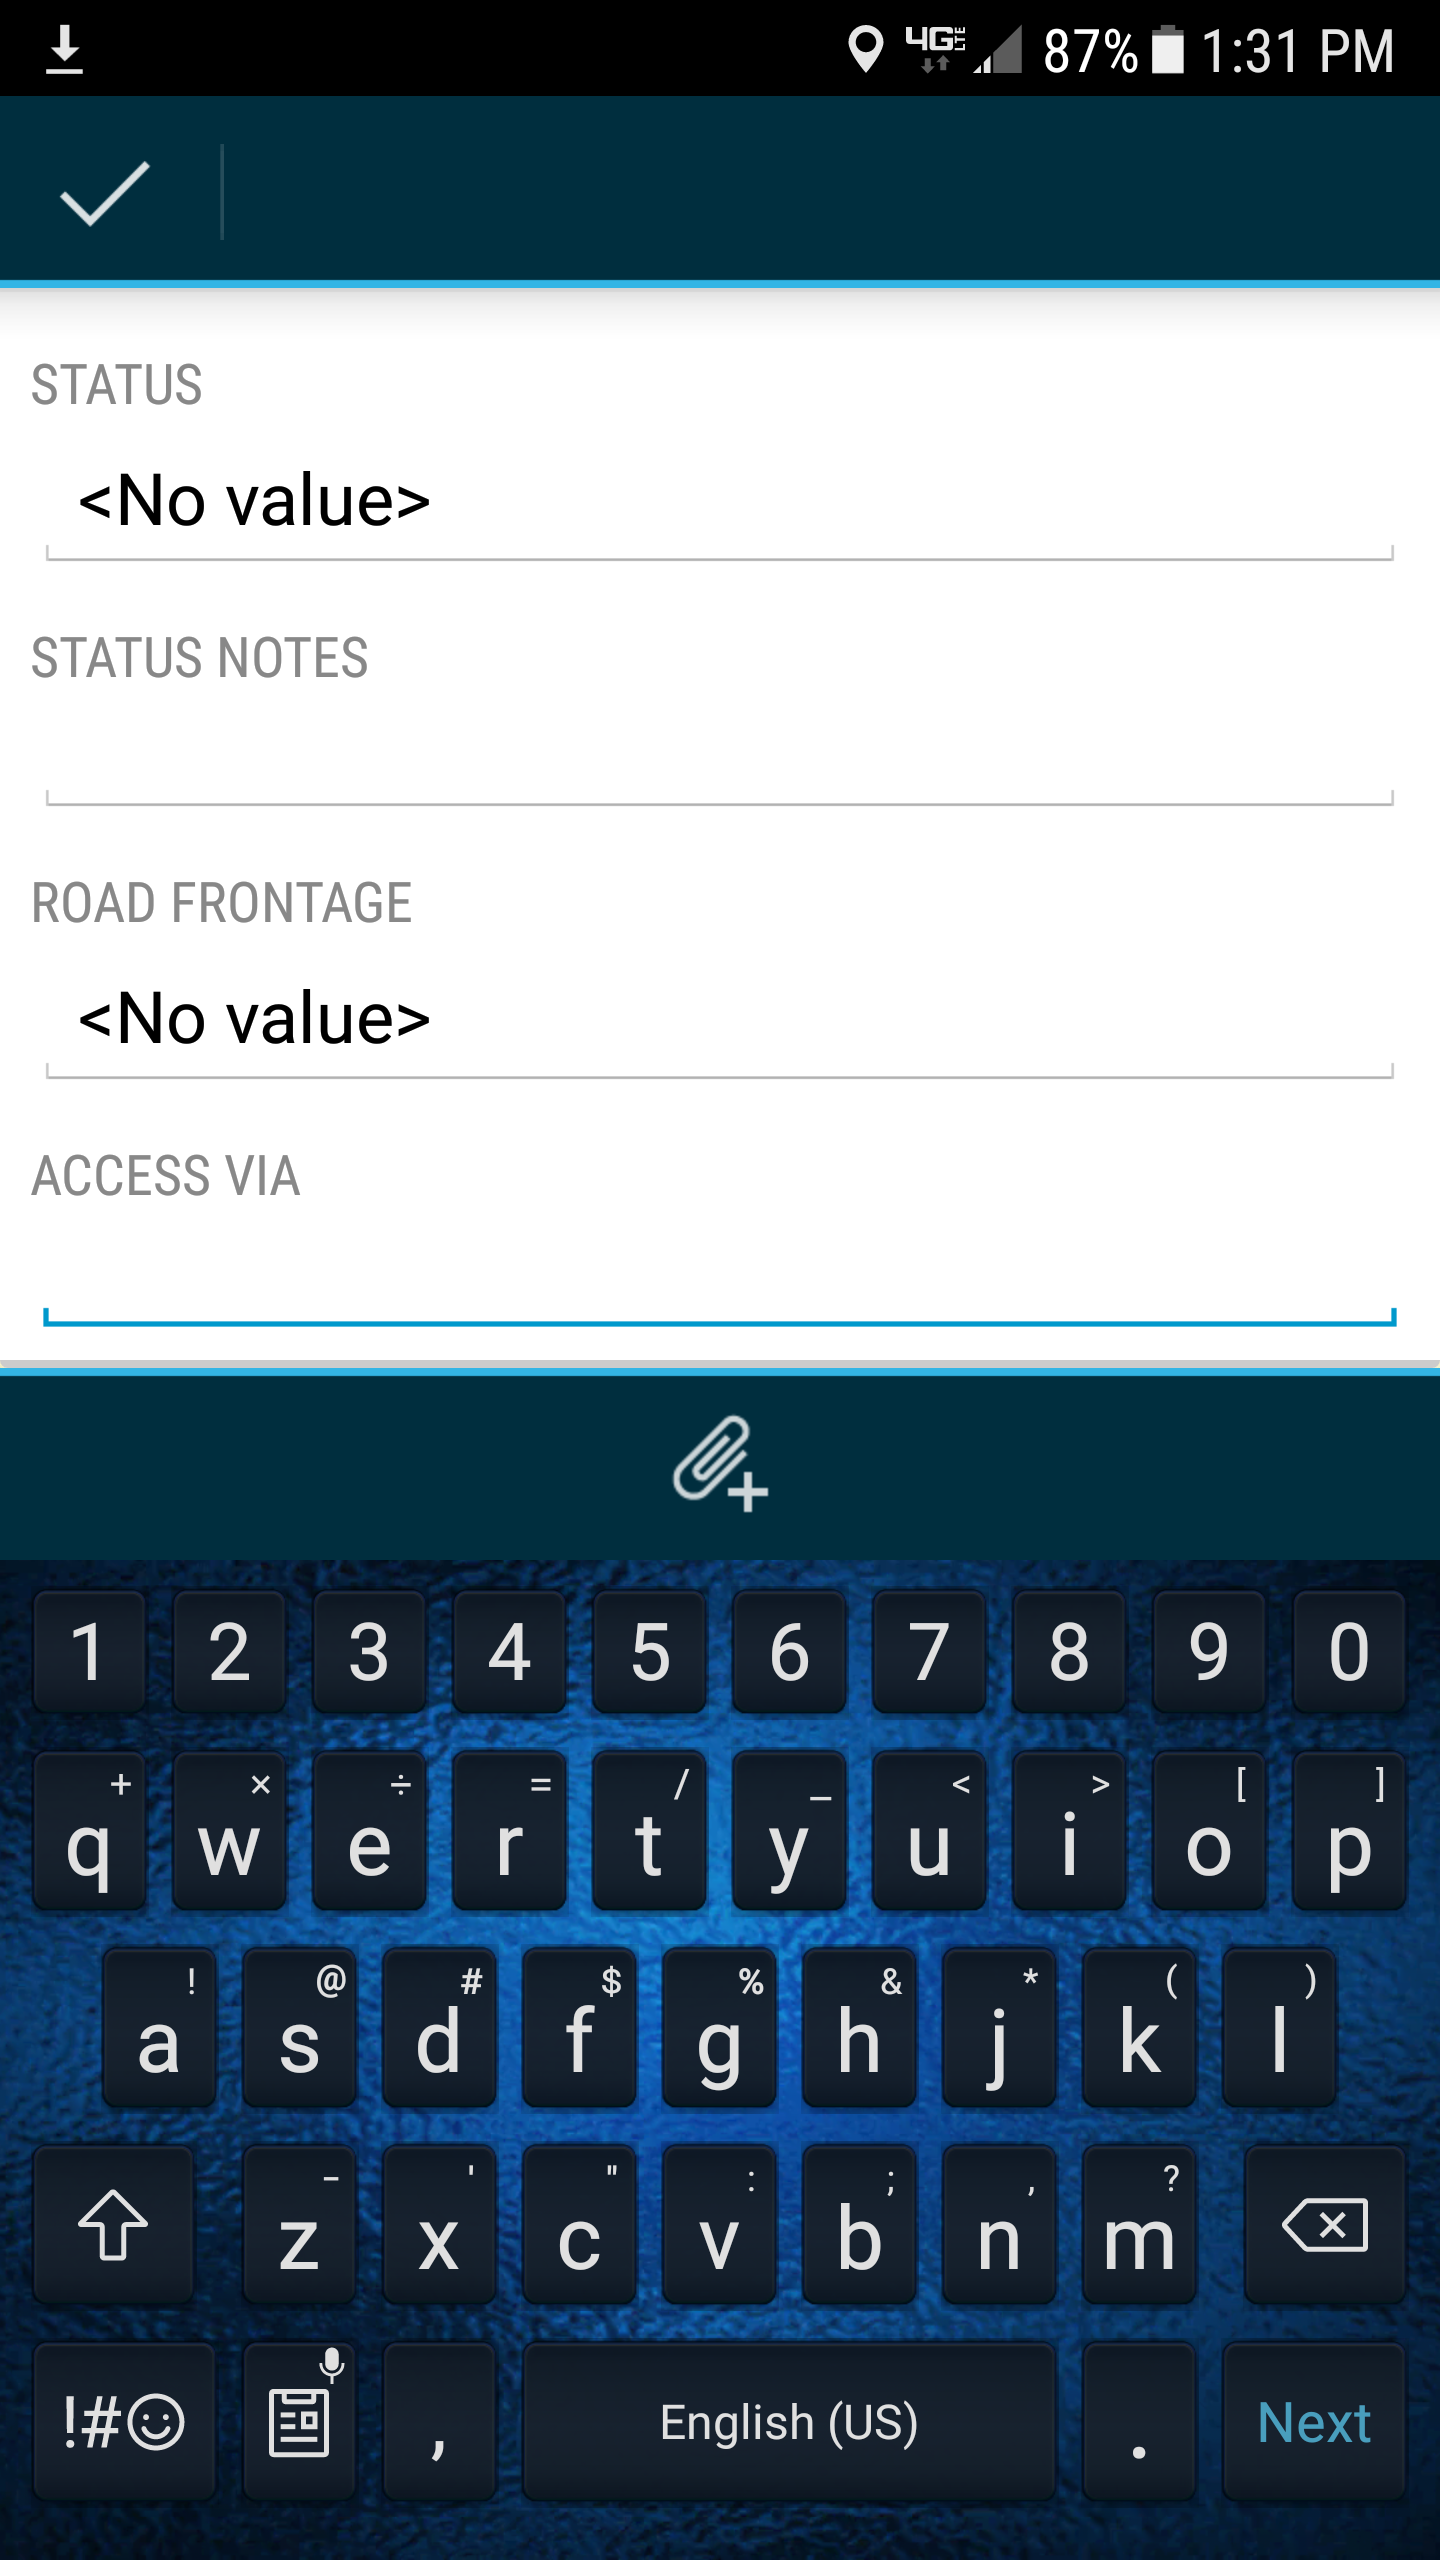
\includegraphics[width=.2\textwidth]{accessVia.png}
\caption {Access Via}
\vspace{.2in}
\HRule \\[.4cm] % Horizontal Line added
\vspace{.2in}
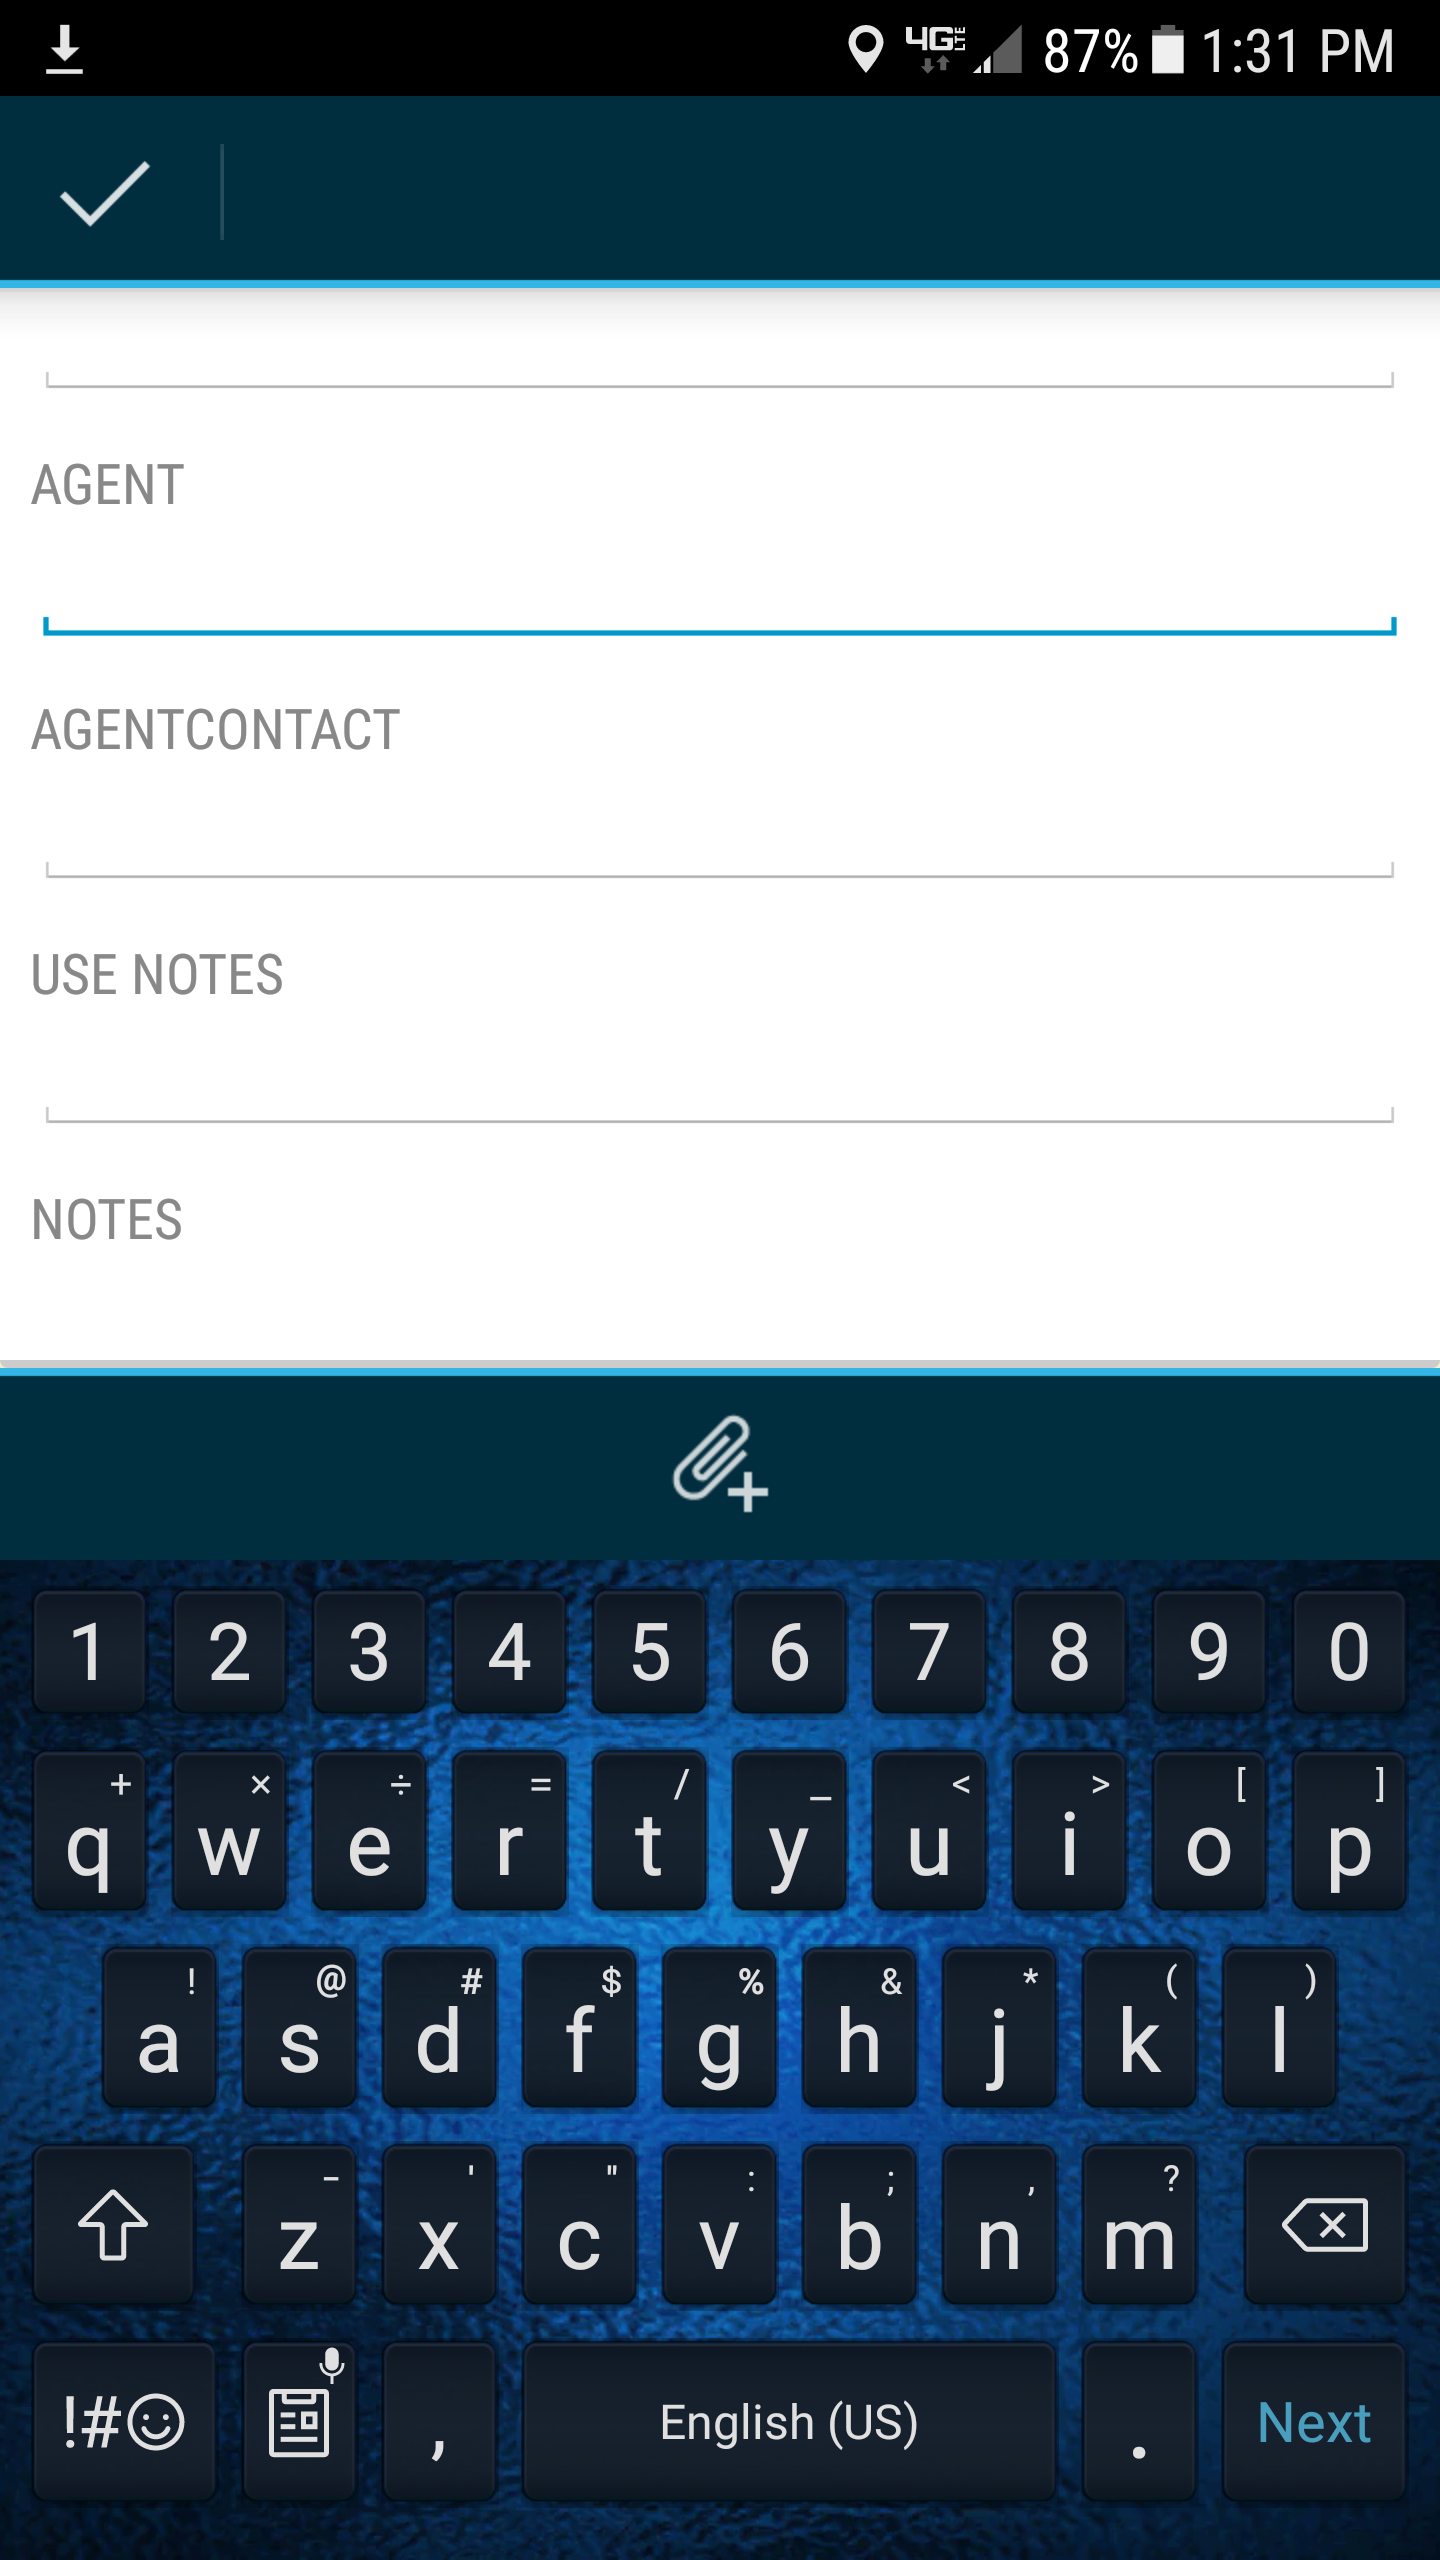
\includegraphics[width=.2\textwidth]{agent.png}
\caption{Agent}
\vspace{.2in}
\HRule \\[.4cm] % Horizontal Line added
\vspace{.2in}
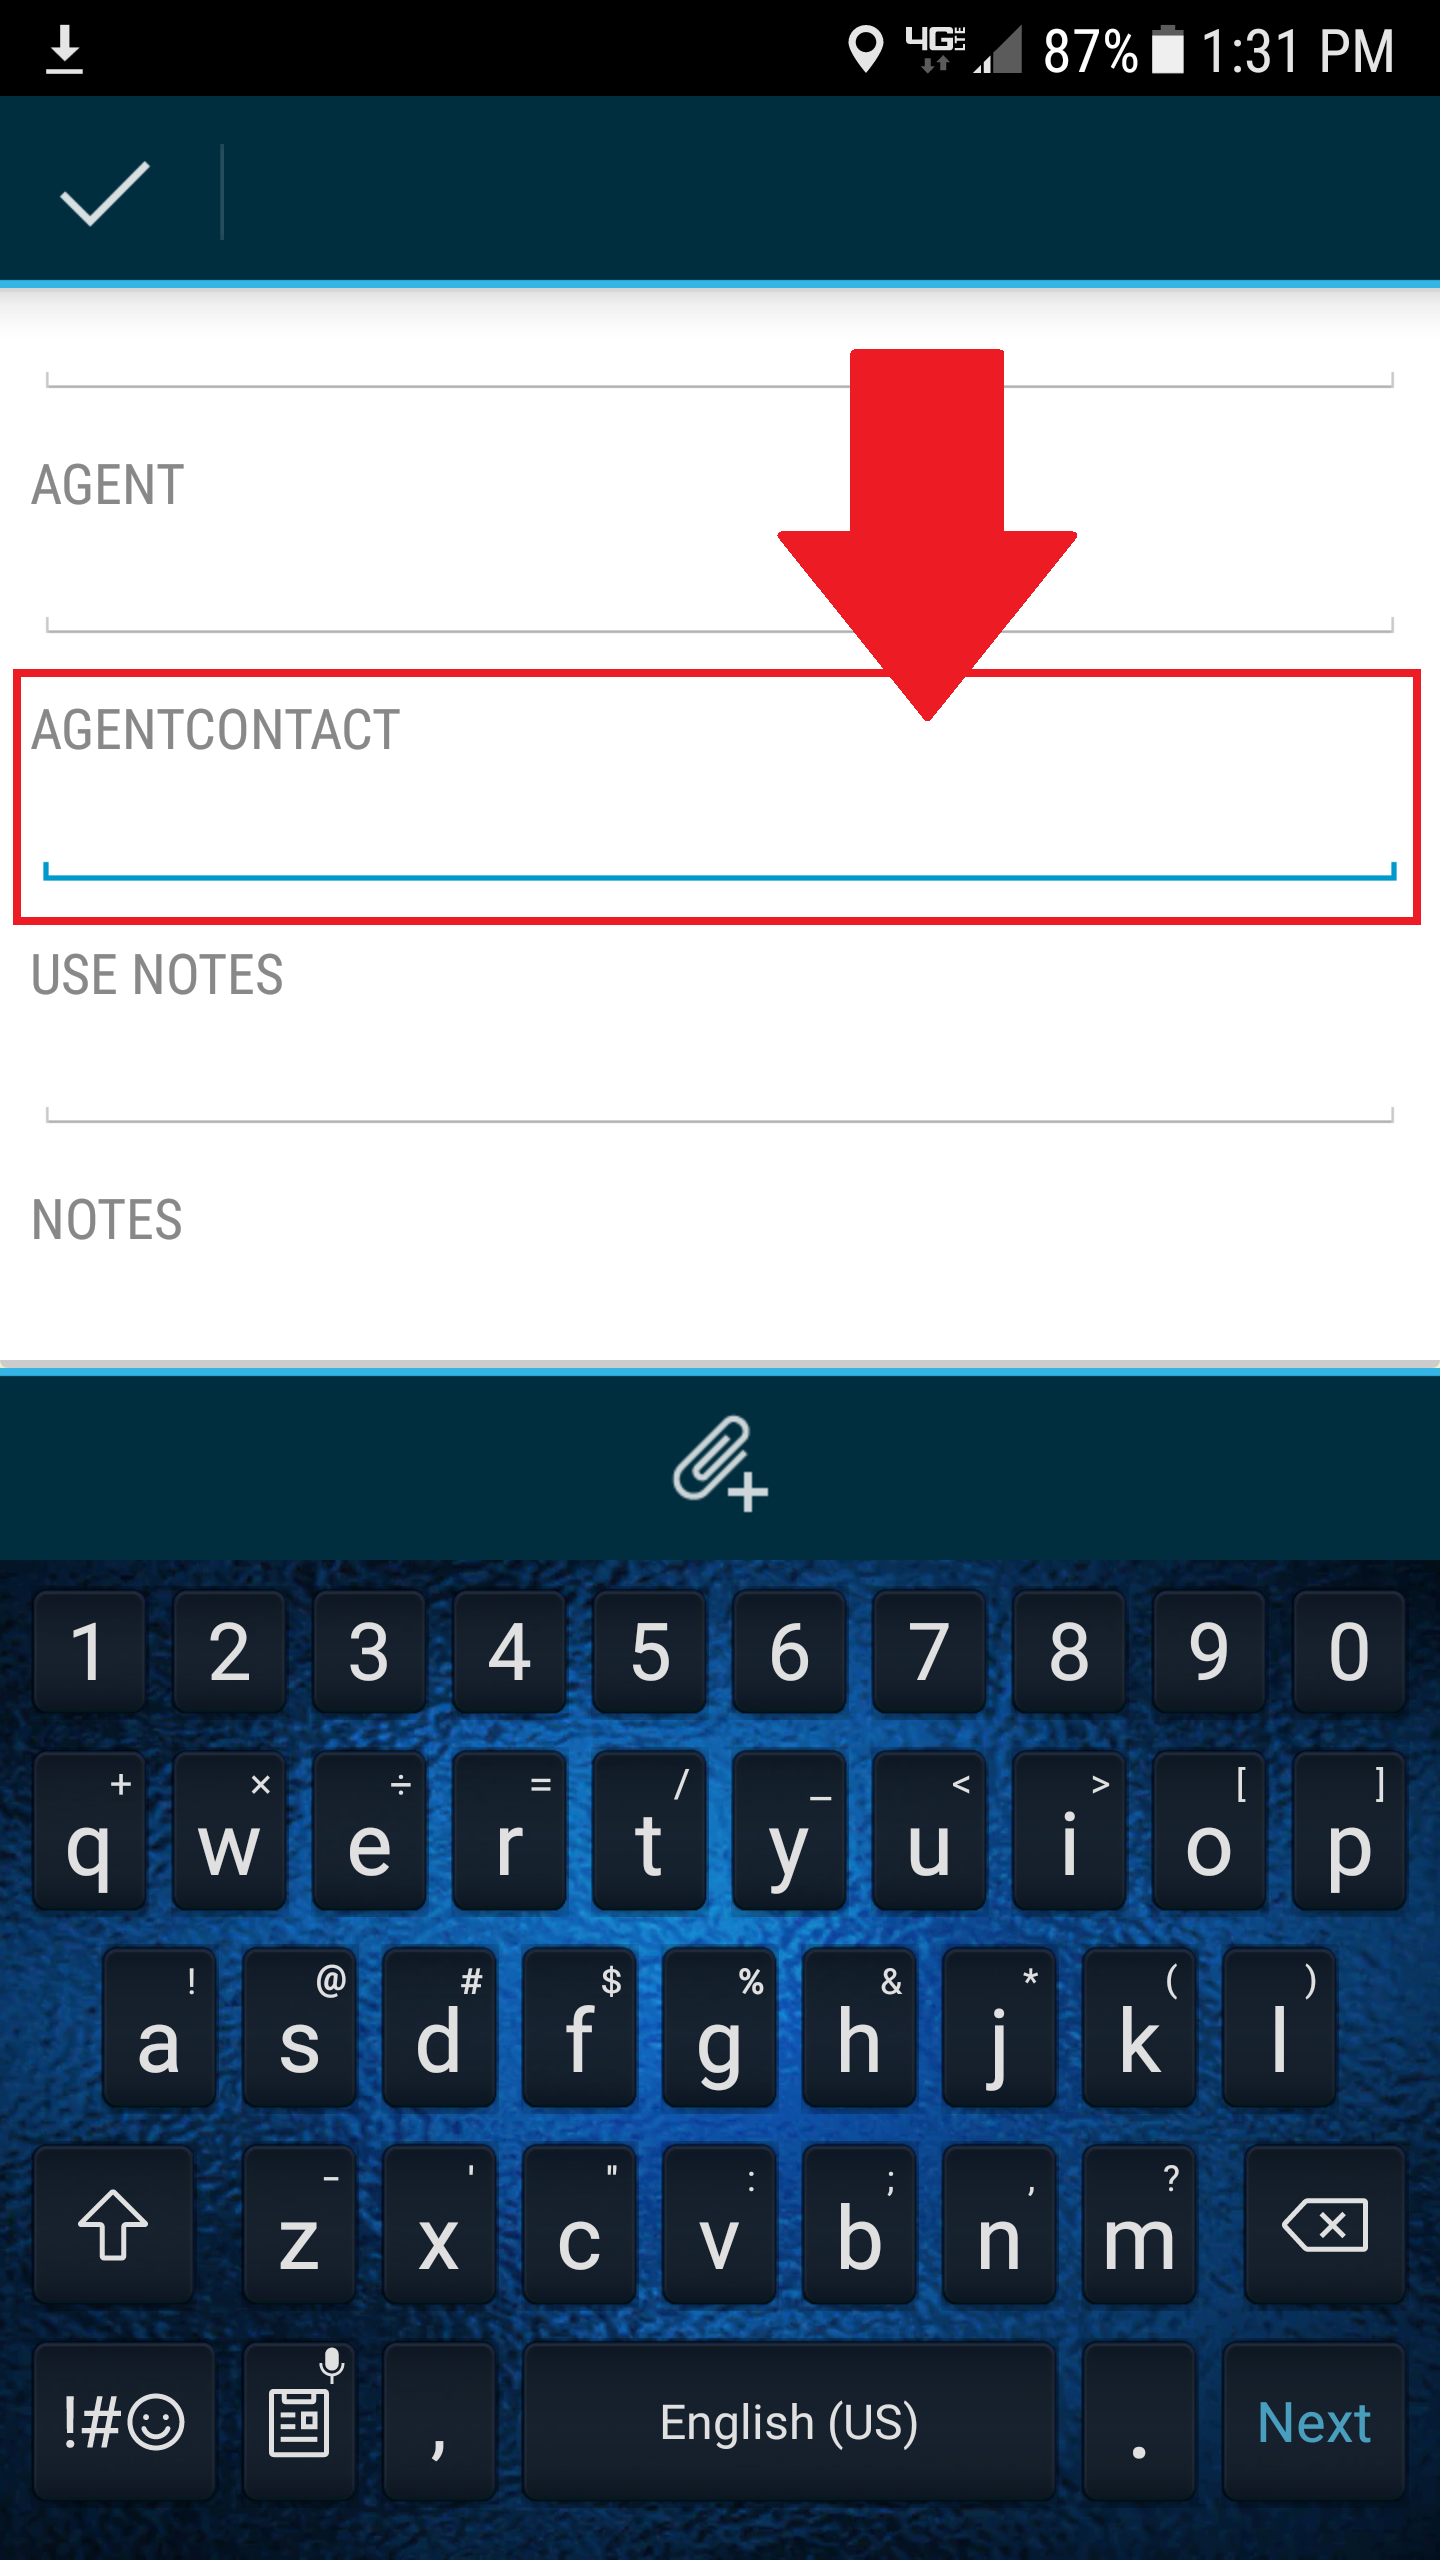
\includegraphics[width=.2\textwidth]{agentContact.png}
\caption{Agent Contact}
\end{wrapfigure}
Enter road used for access\\
\vspace{2in}

\noindent Enter Agent Name\\
\vspace{2in}

\noindent Enter Agent Contact Info\\

\clearpage
\subparagraph*{Device 1 Field Operation Cont.}
\subparagraph*{\\}
\begin{wrapfigure}{r}{0.5\textwidth}
\centering
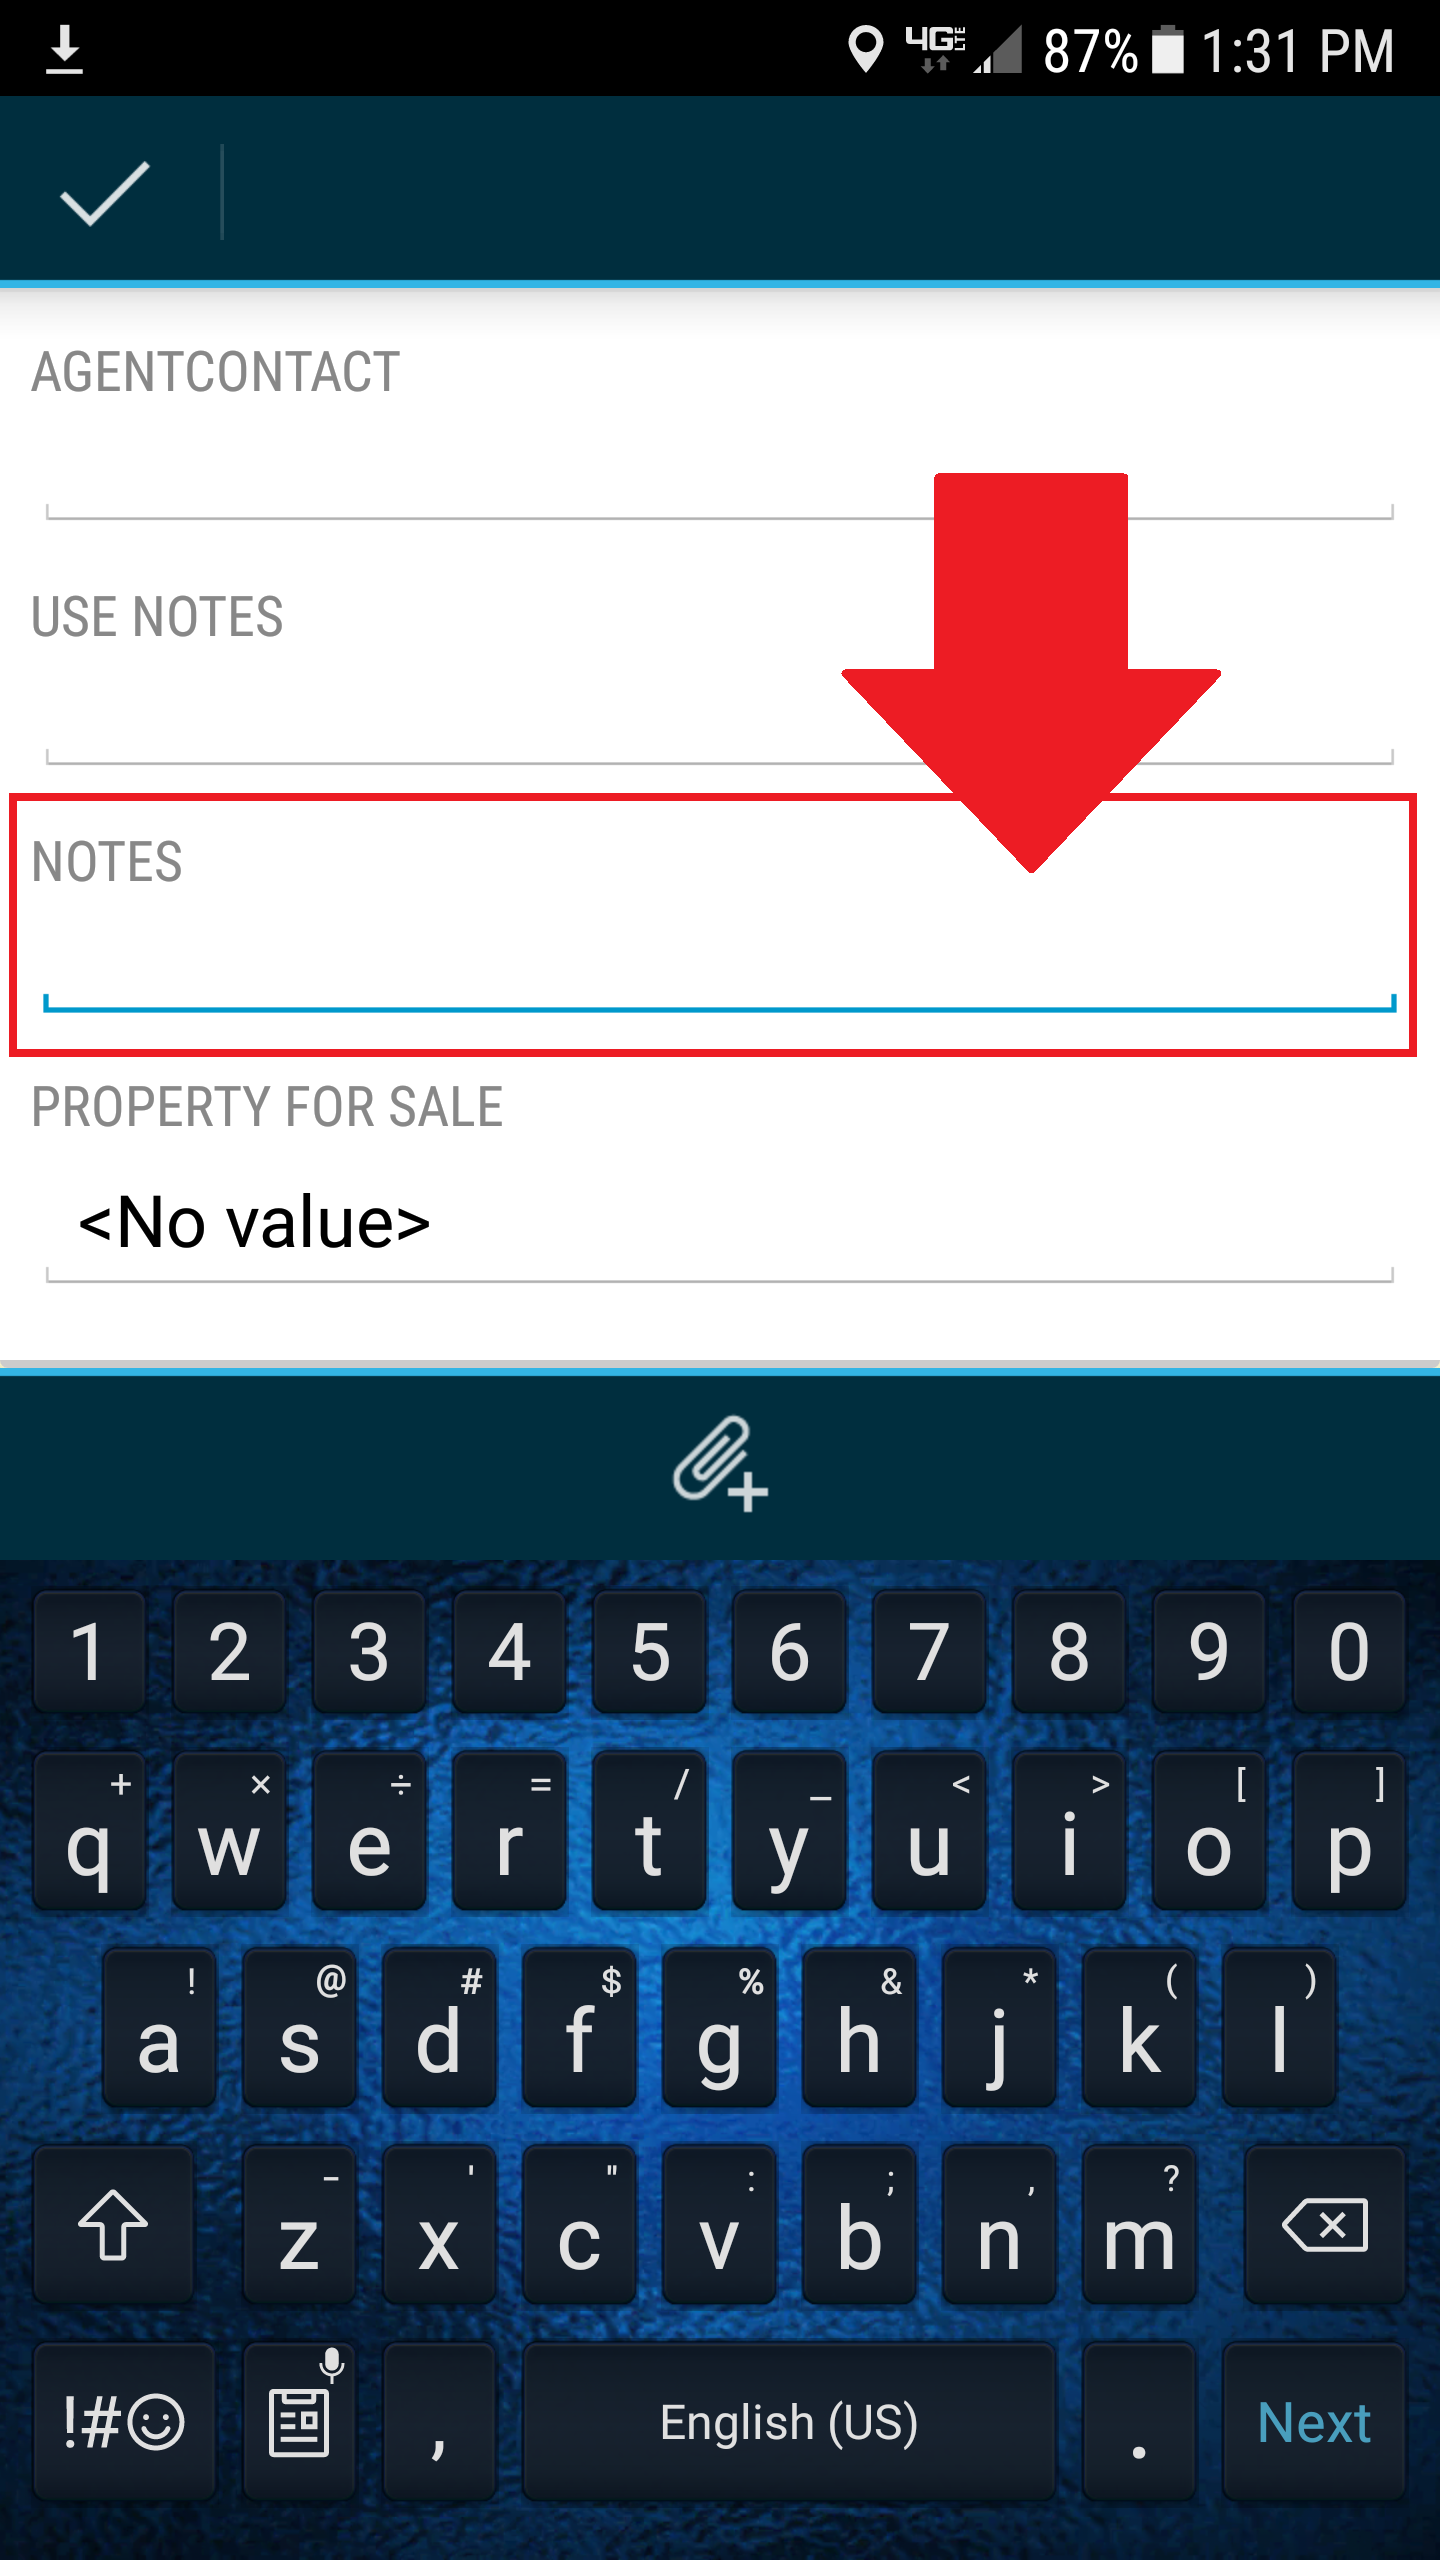
\includegraphics[width=.2\textwidth]{notes.png}
\caption {Use Notes}
\vspace{.2in}
\HRule \\[.4cm] % Horizontal Line added
\vspace{.2in}
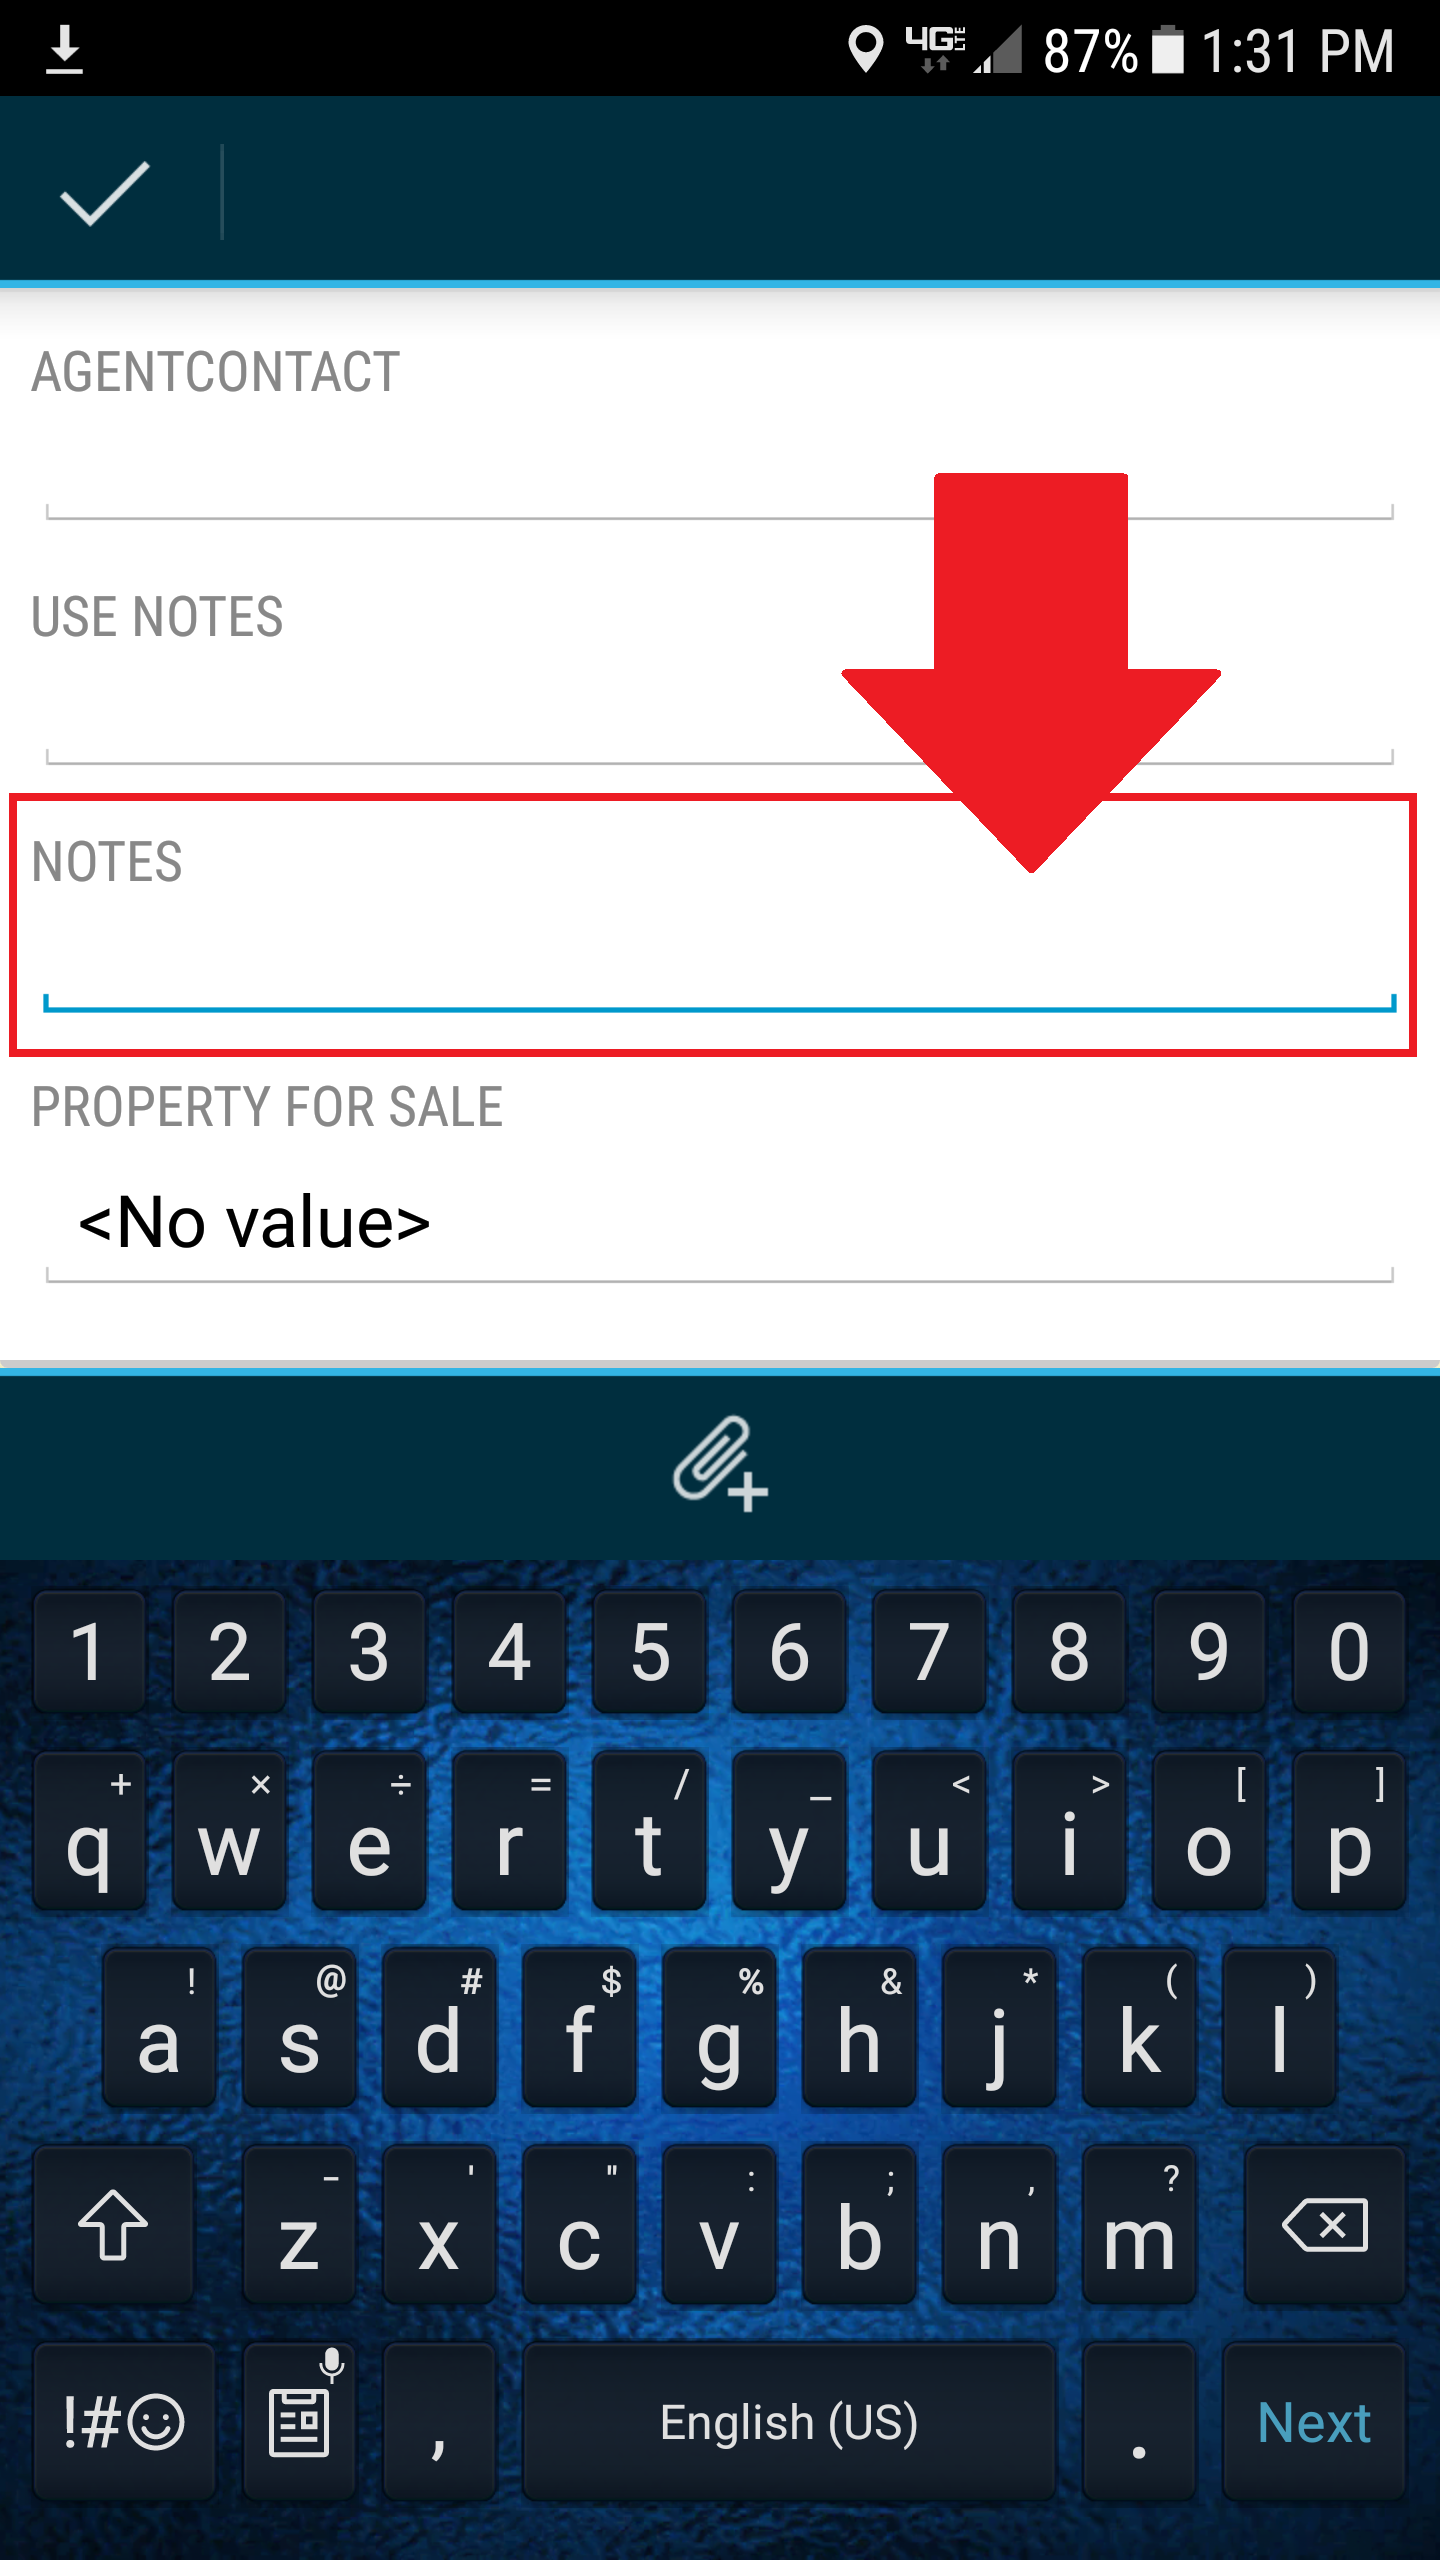
\includegraphics[width=.2\textwidth]{notes.png}
\caption{Notes}
\vspace{.2in}
\HRule \\[.4cm] % Horizontal Line added
\vspace{.2in}
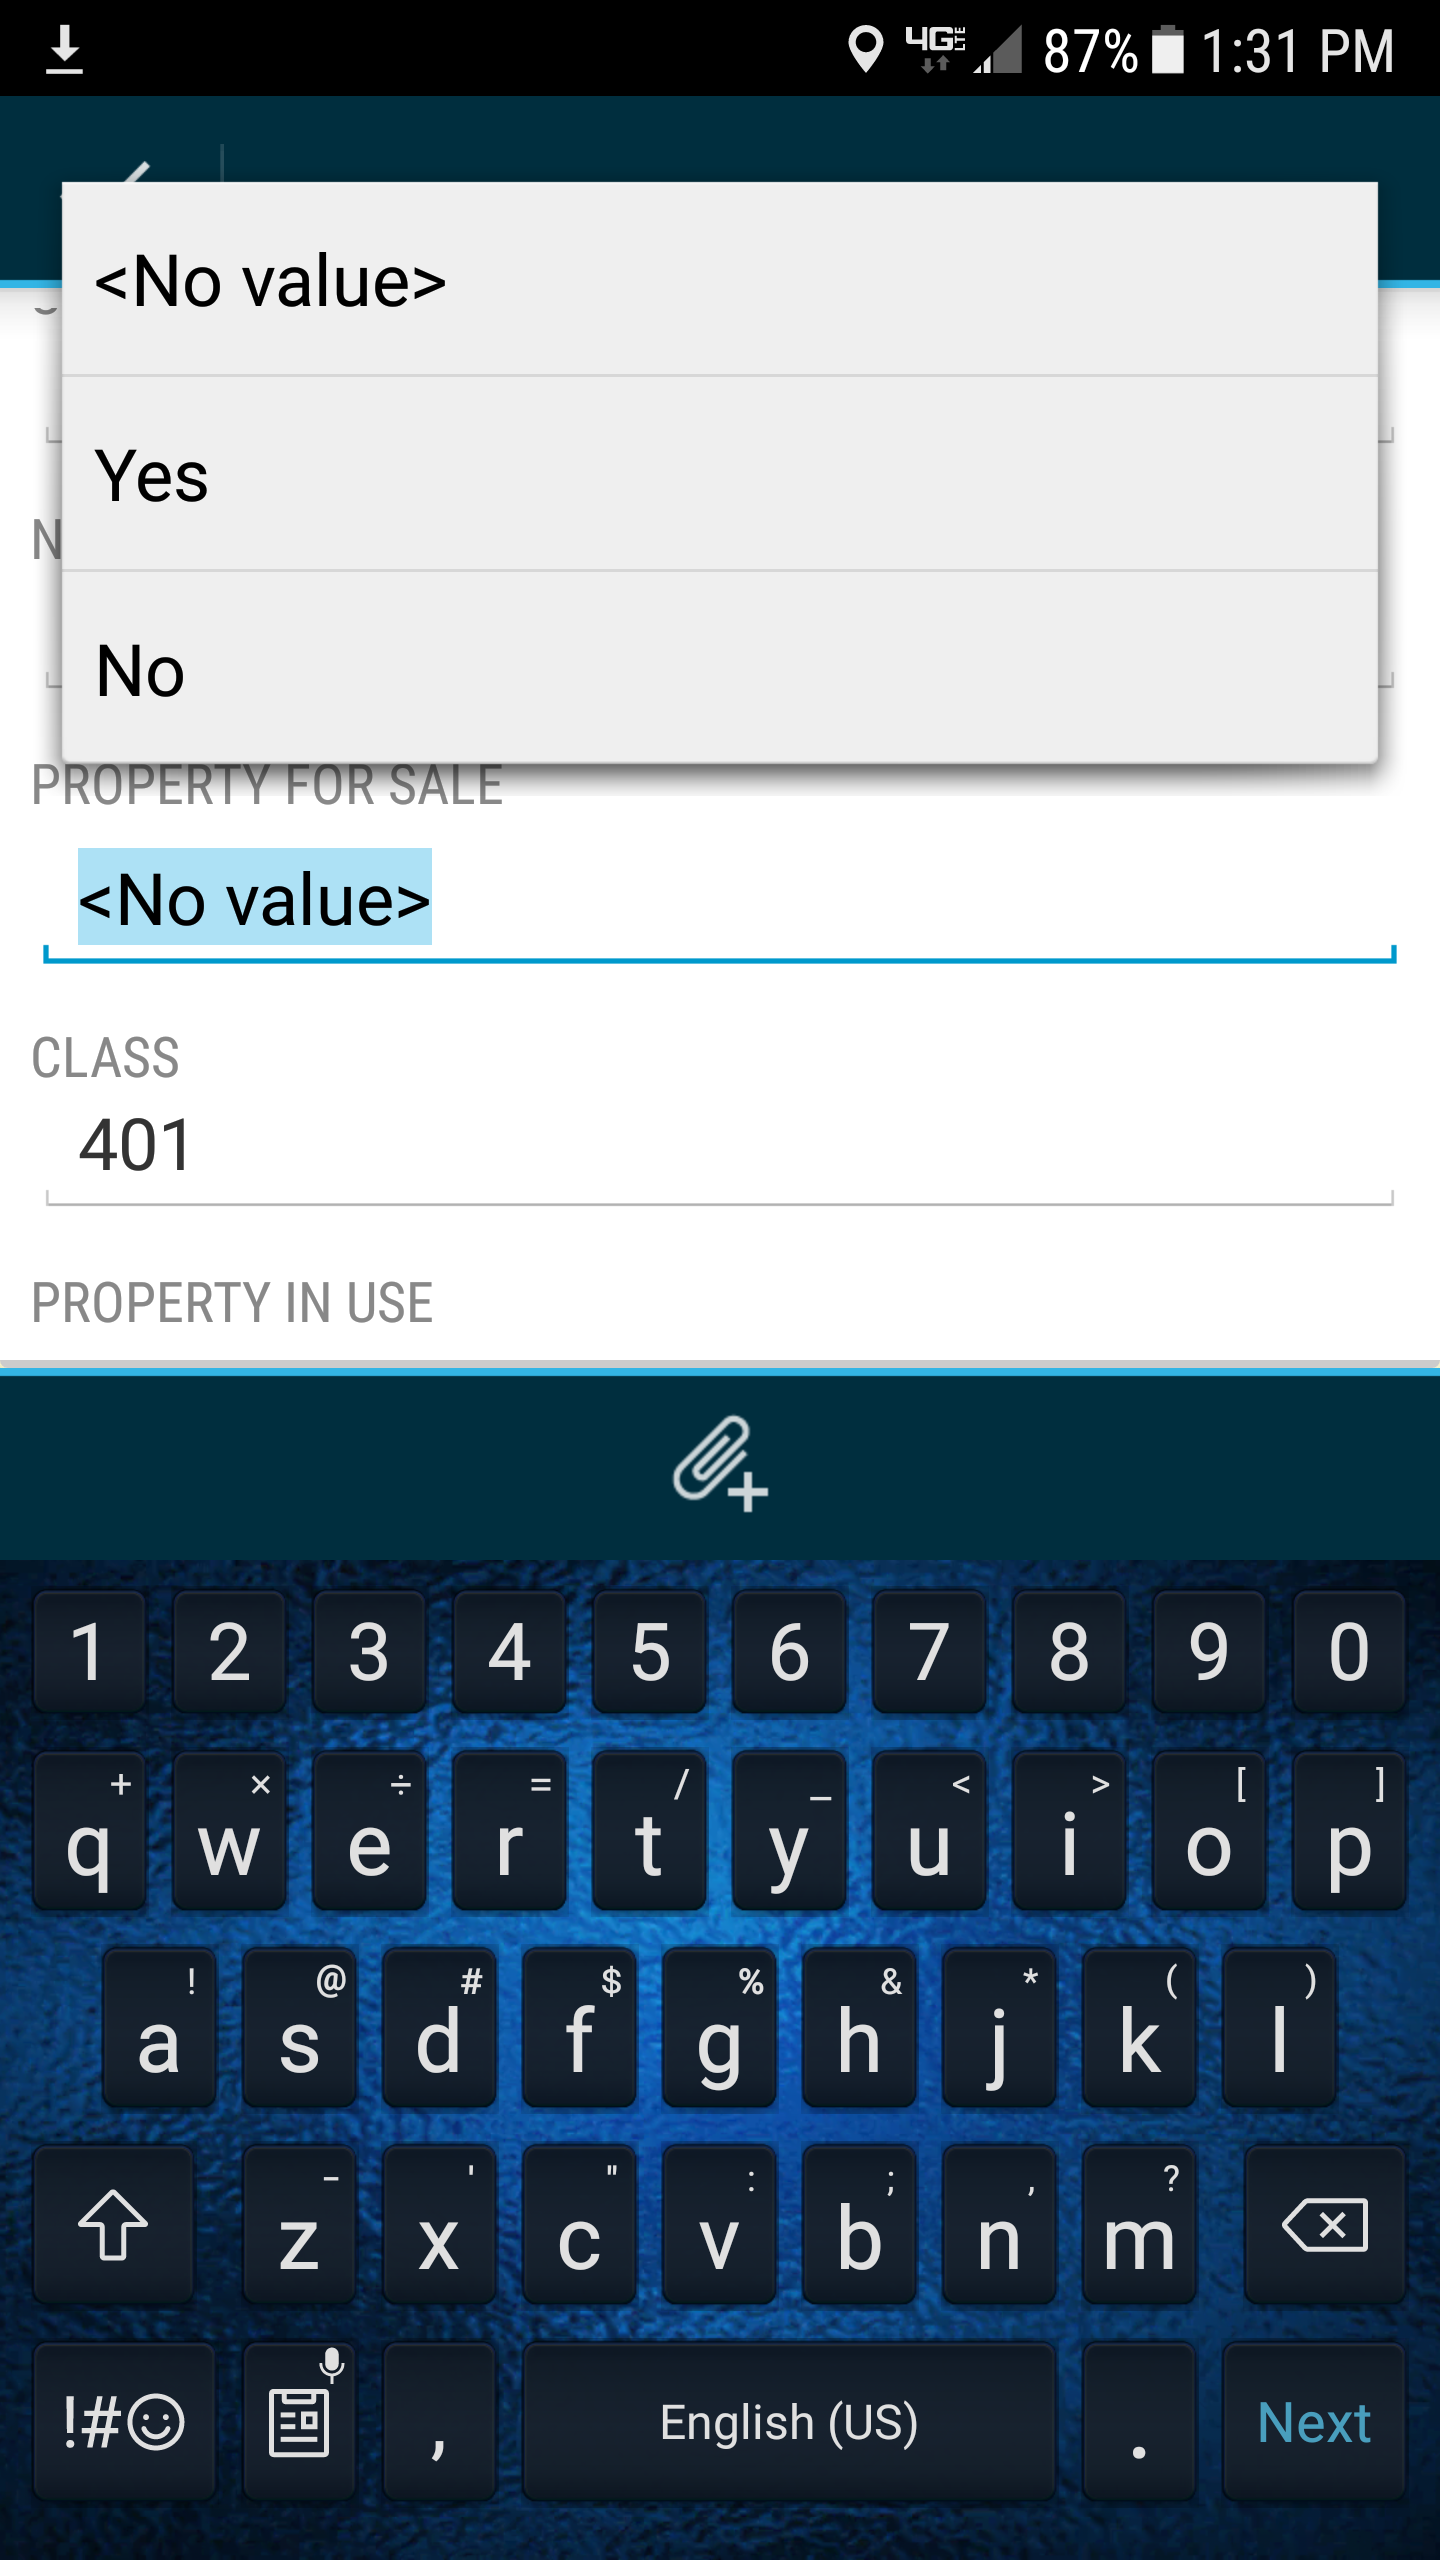
\includegraphics[width=.2\textwidth]{propertyForSale.png}
\caption{Property for Sale}
\end{wrapfigure}
Enter  Use Notes up to 120 characters\\
\vspace{2in}
\noindent Enter Notes up to 120 characters\\
\vspace{2in}
\noindent Enter property for sale yes or no\\
\clearpage
\subparagraph*{Device 1 Field Operation Cont.}
\subparagraph*{\\}
\begin{wrapfigure}{r}{0.5\textwidth}
\centering
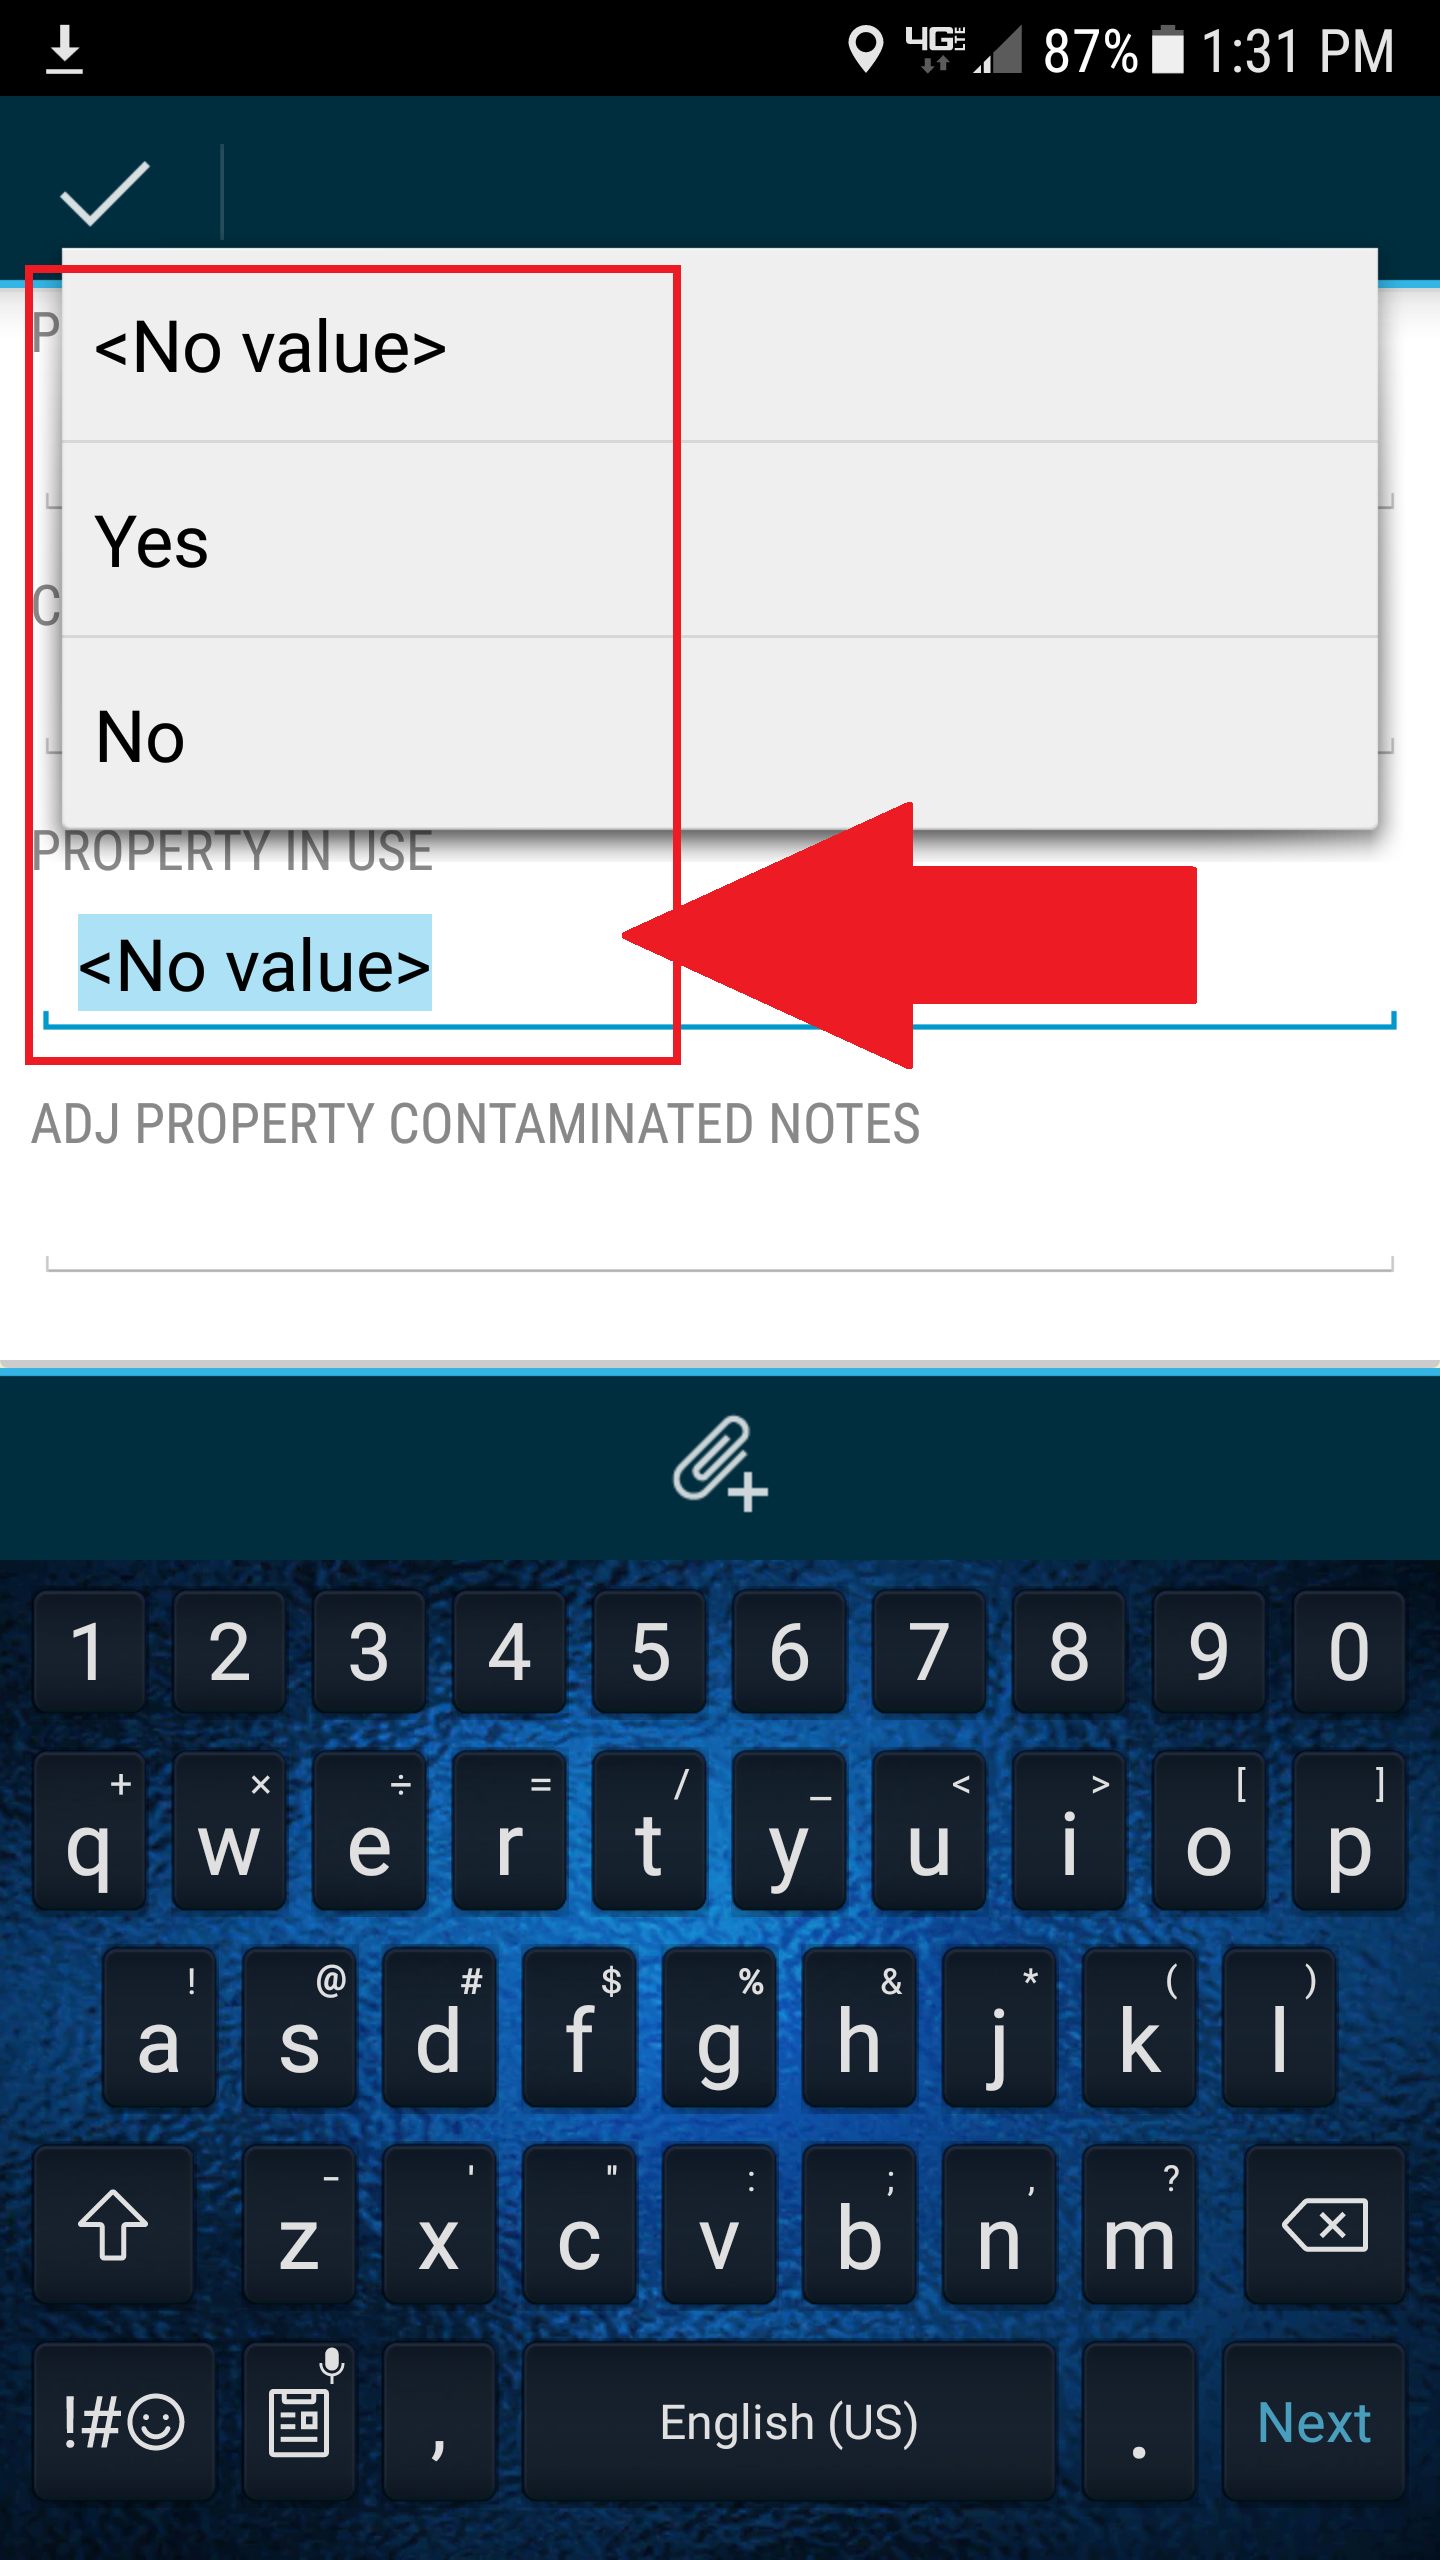
\includegraphics[width=.2\textwidth]{propertyInUse.png}
\caption {Property in Use}
\vspace{.2in}
\HRule \\[.4cm] % Horizontal Line added
\vspace{.2in}
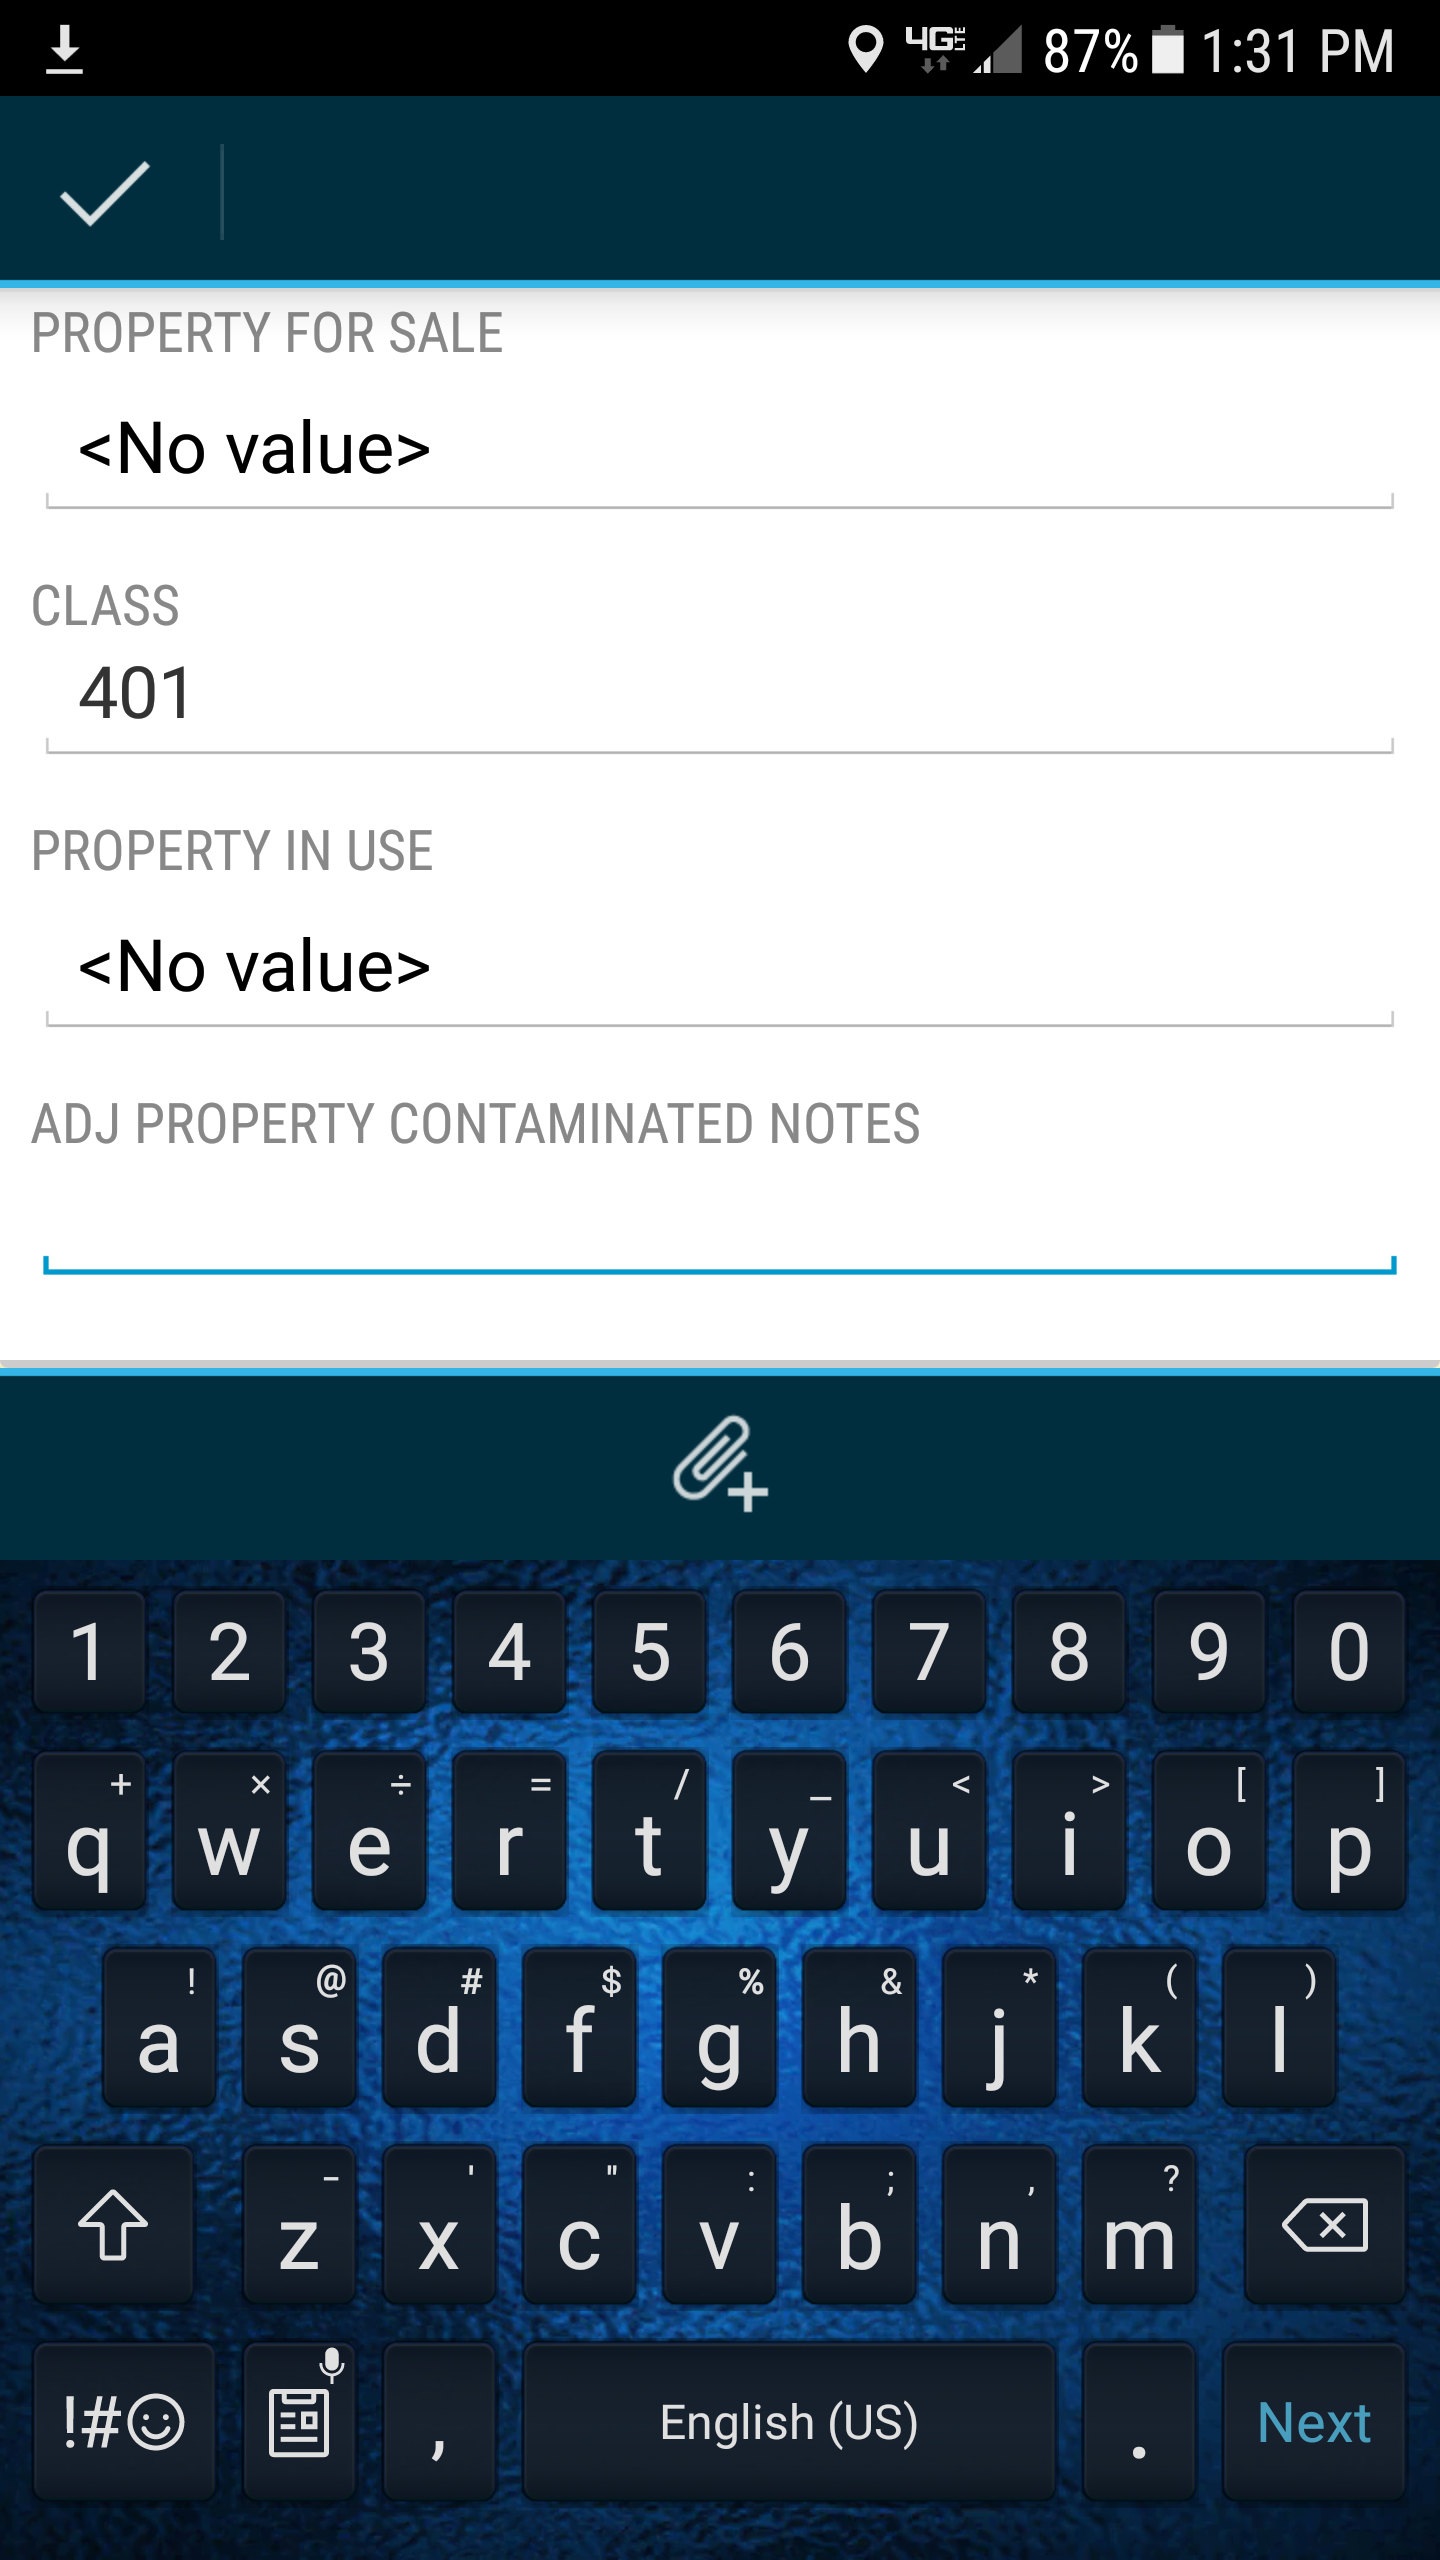
\includegraphics[width=.2\textwidth]{adjPropertyContNotes.png}
\caption{Adjacent Property Contaminated Notes}
\vspace{.2in}
\HRule \\[.4cm] % Horizontal Line added
\vspace{.2in}
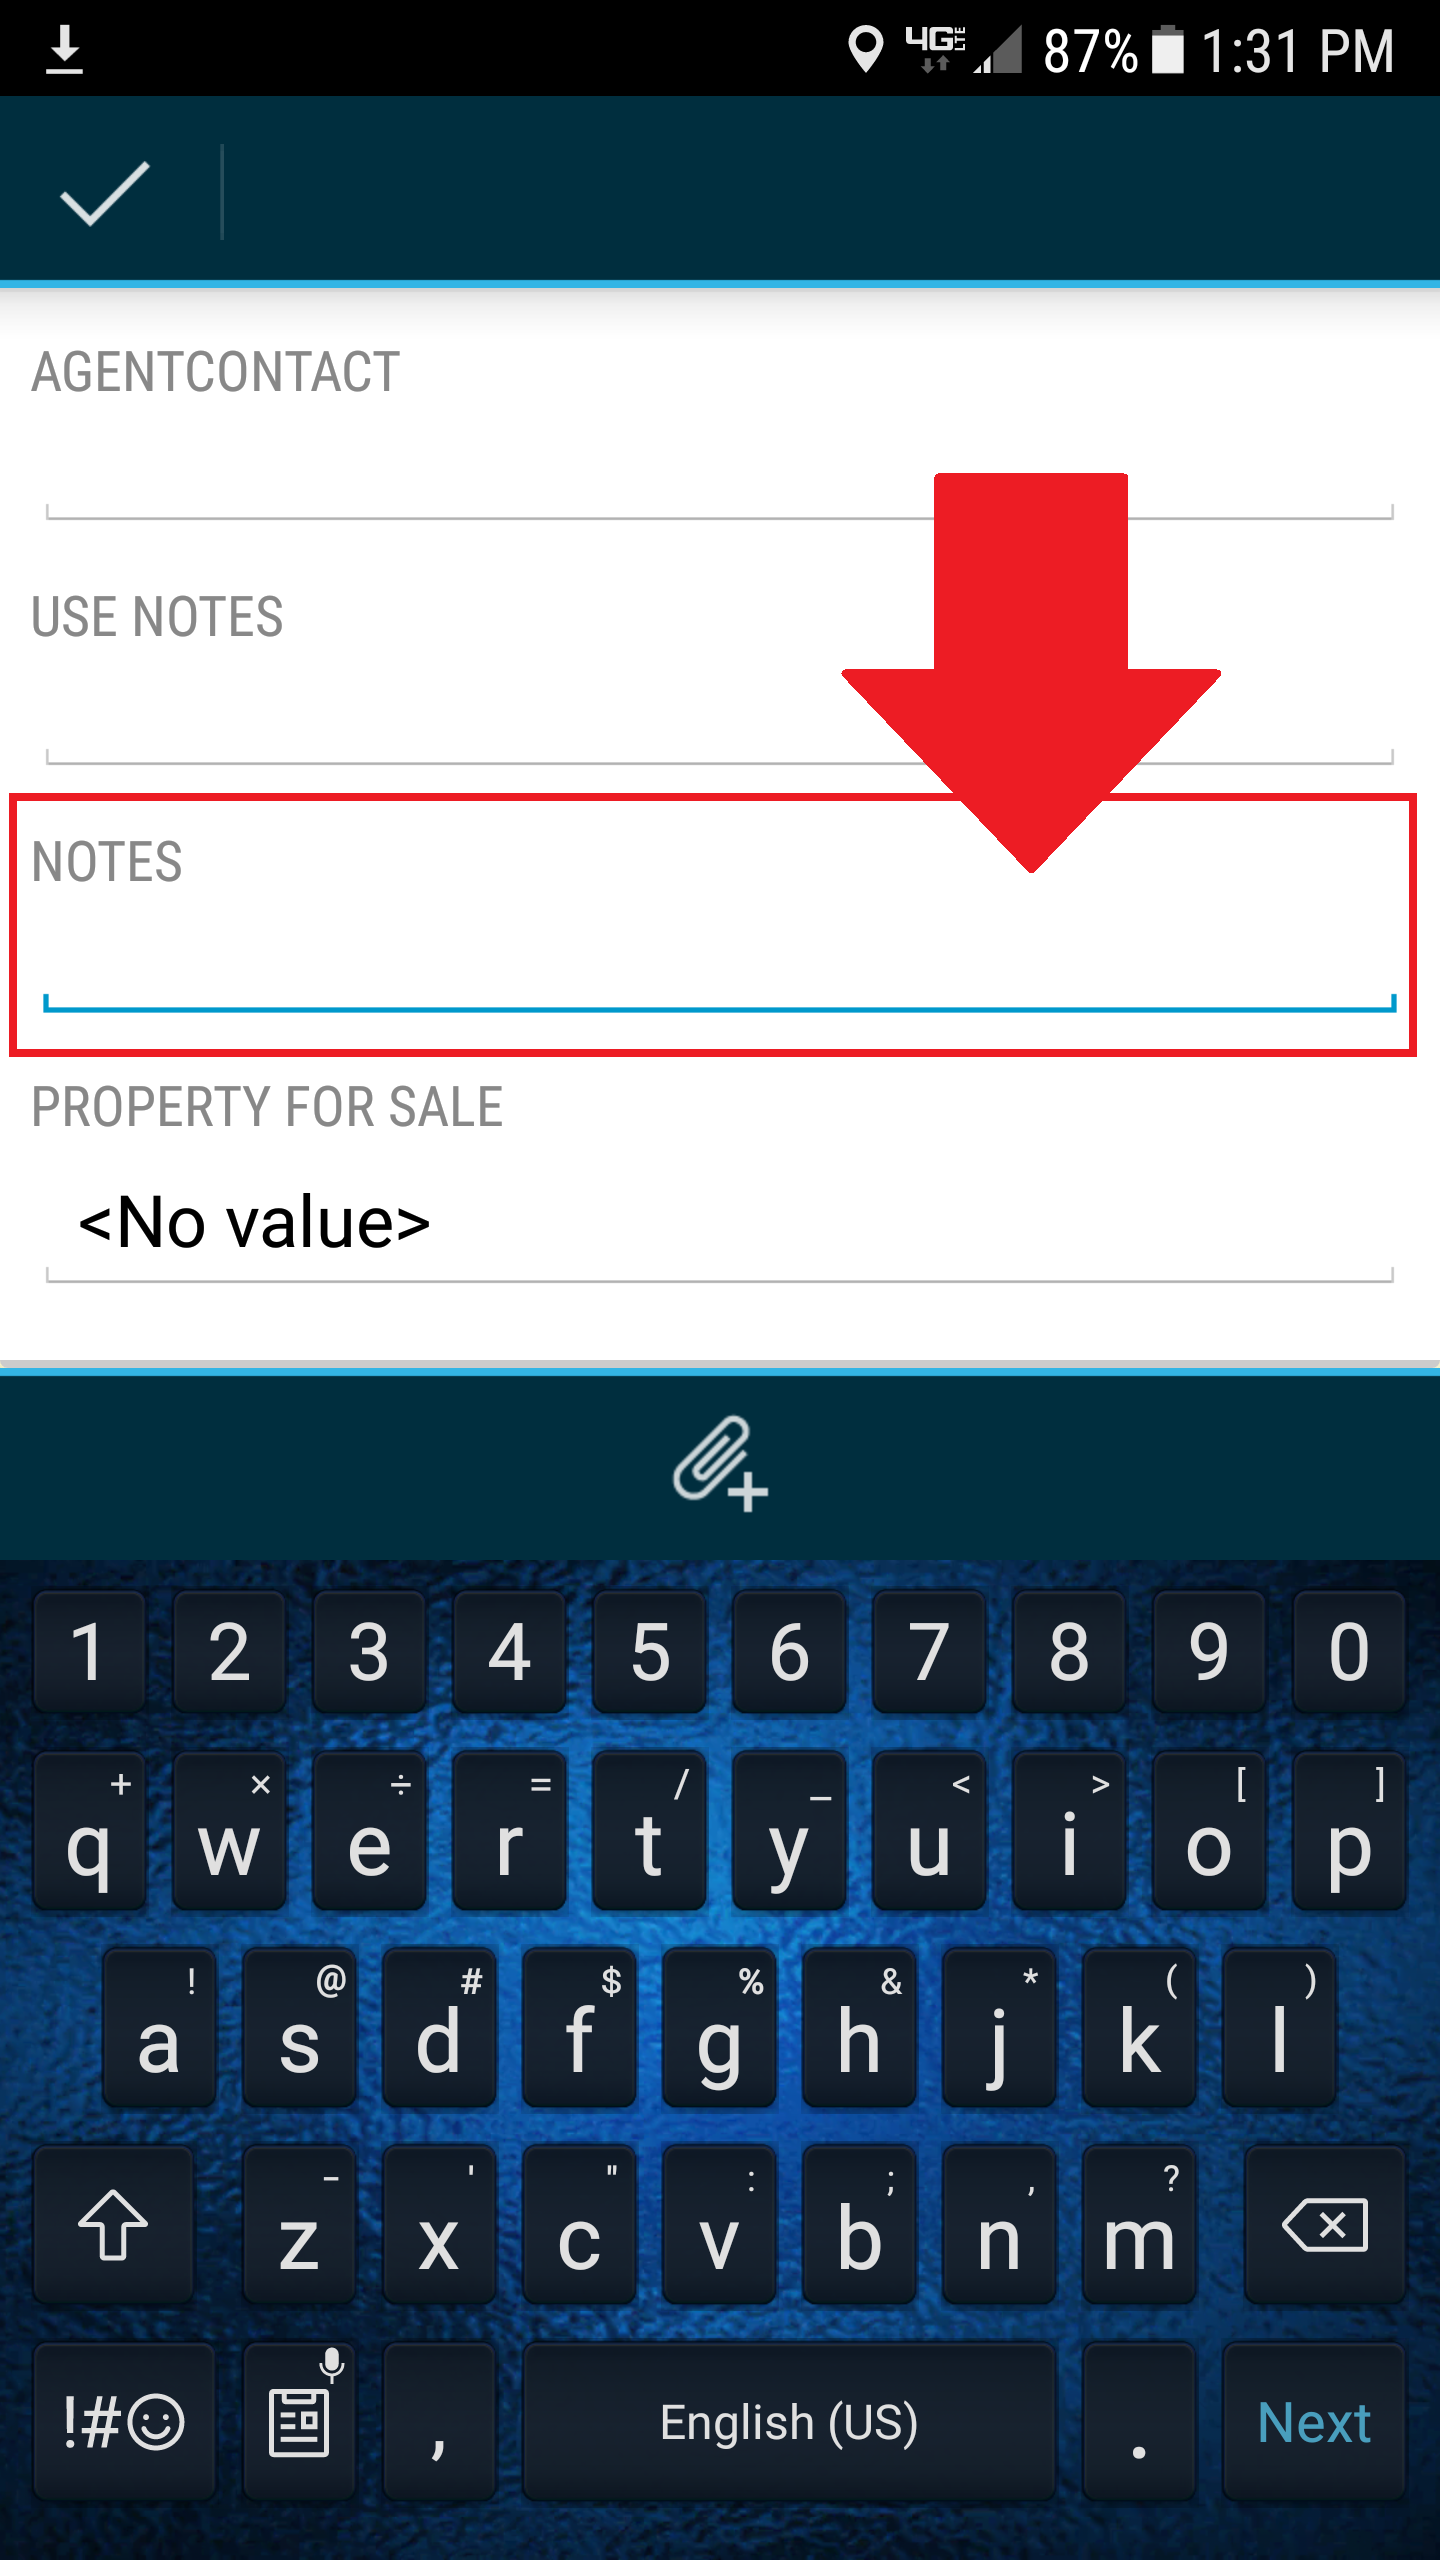
\includegraphics[width=.2\textwidth]{notes.png}
\caption{Property Contaminated}
\end{wrapfigure}
Property in Use Yes or No\\
\vspace{2in}
\noindent Adjacent Property Contaminated Notes up to 120 characters\\
\vspace{2in}
\noindent Property Contaminated yes or no prefilled\\
\clearpage
\subparagraph*{Device 1 Field Operation Cont.}
\subparagraph*{\\}
\begin{wrapfigure}{r}{0.5\textwidth}
\centering
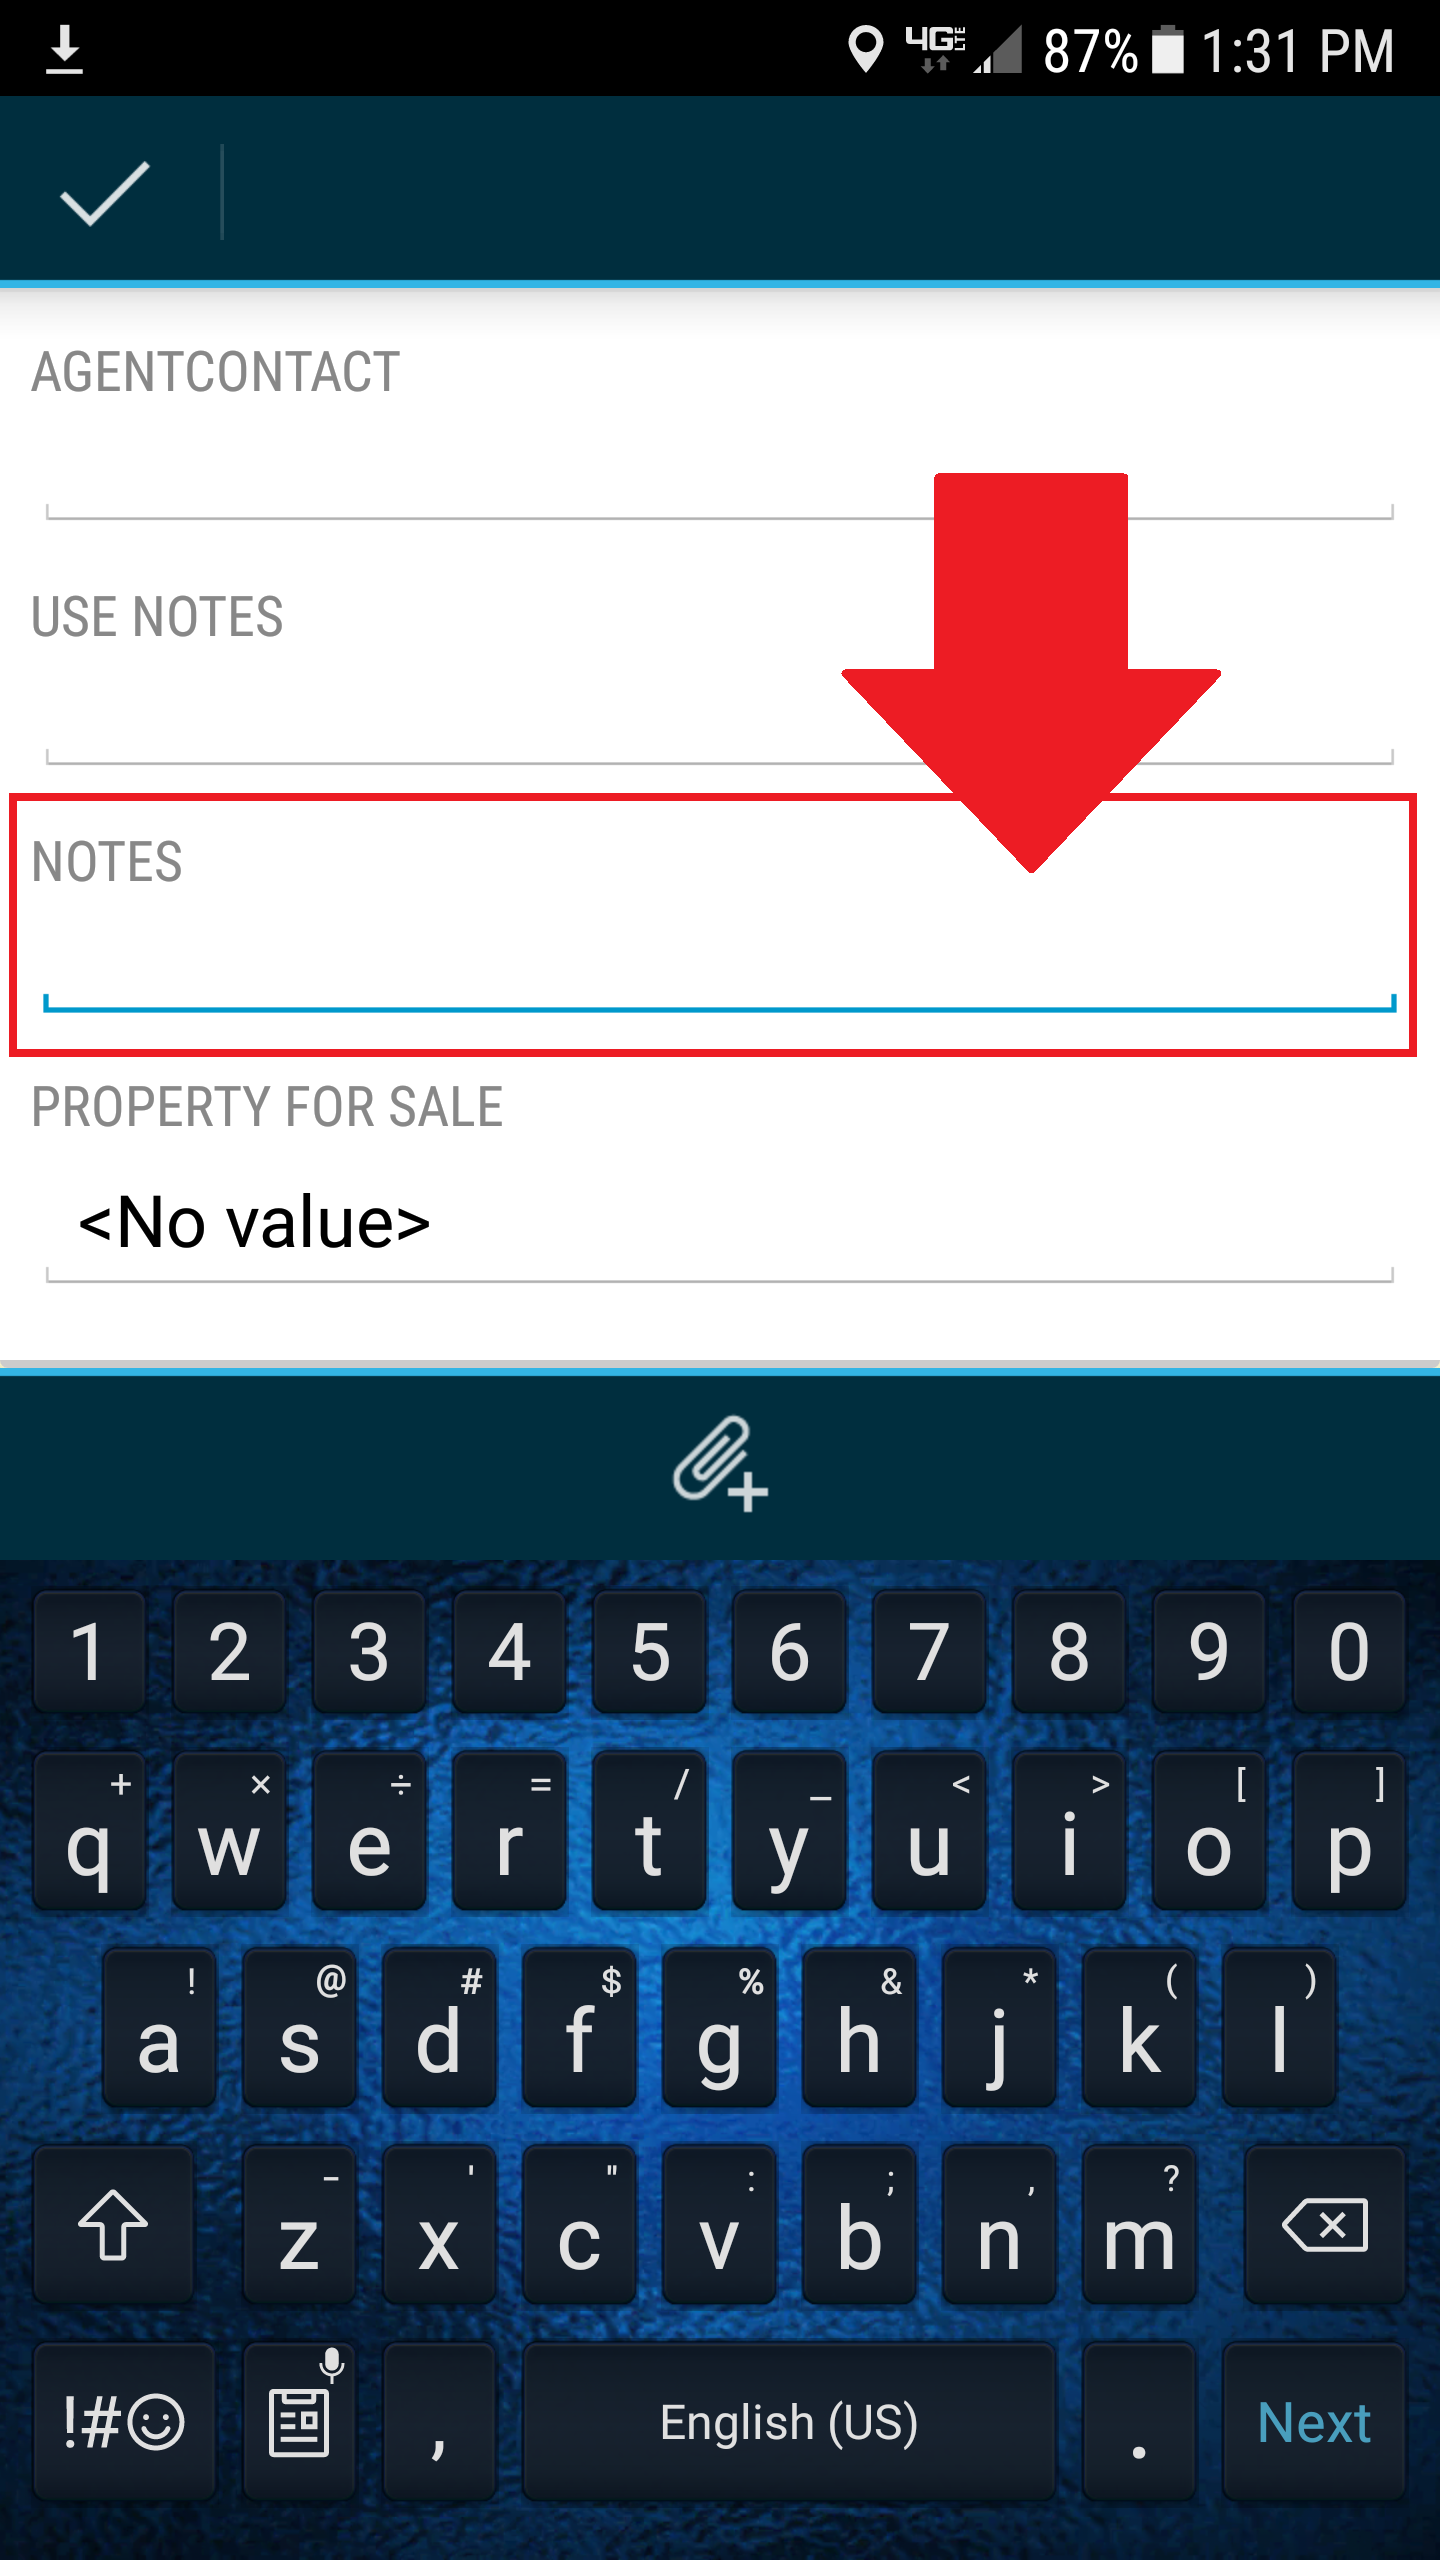
\includegraphics[width=.2\textwidth]{notes.png}
\caption {Notes up to 120 characters}
\vspace{.2in}
\HRule \\[.4cm] % Horizontal Line added
\vspace{.2in}
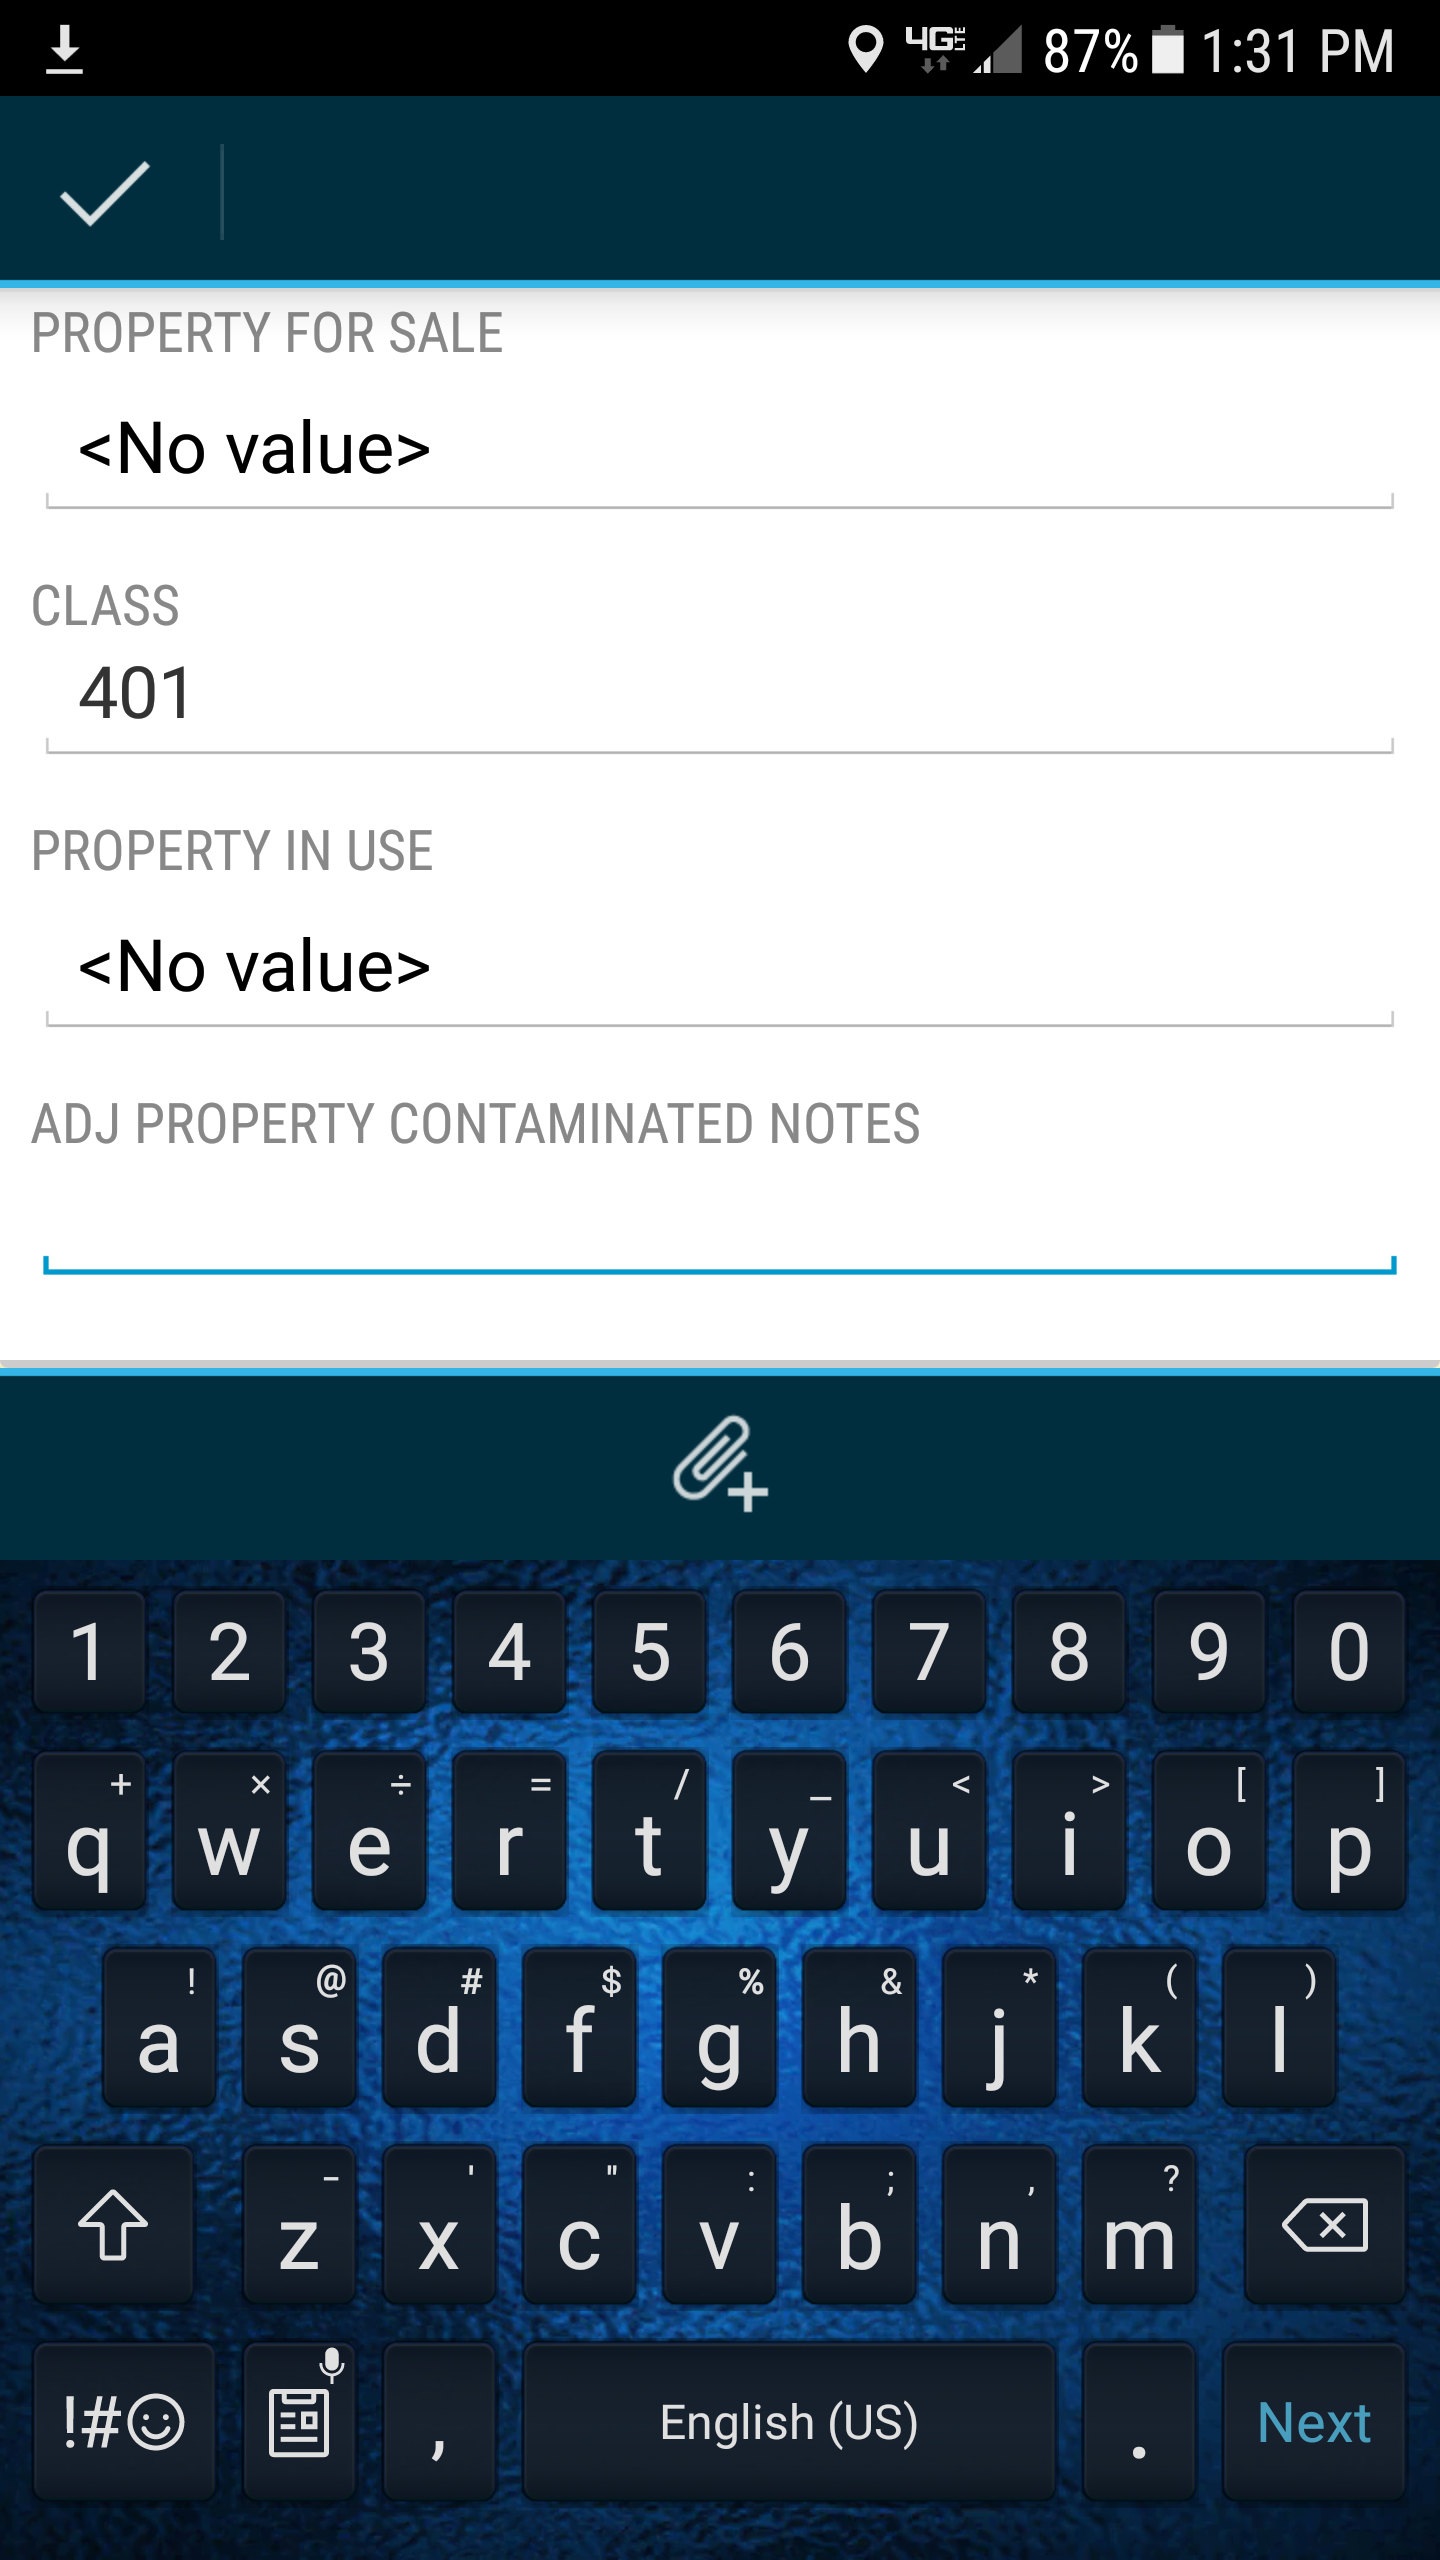
\includegraphics[width=.2\textwidth]{adjPropertyContNotes.png}
\caption{Adjacent Property Contaminated}
\vspace{.2in}
\HRule \\[.4cm] % Horizontal Line added
\vspace{.2in}
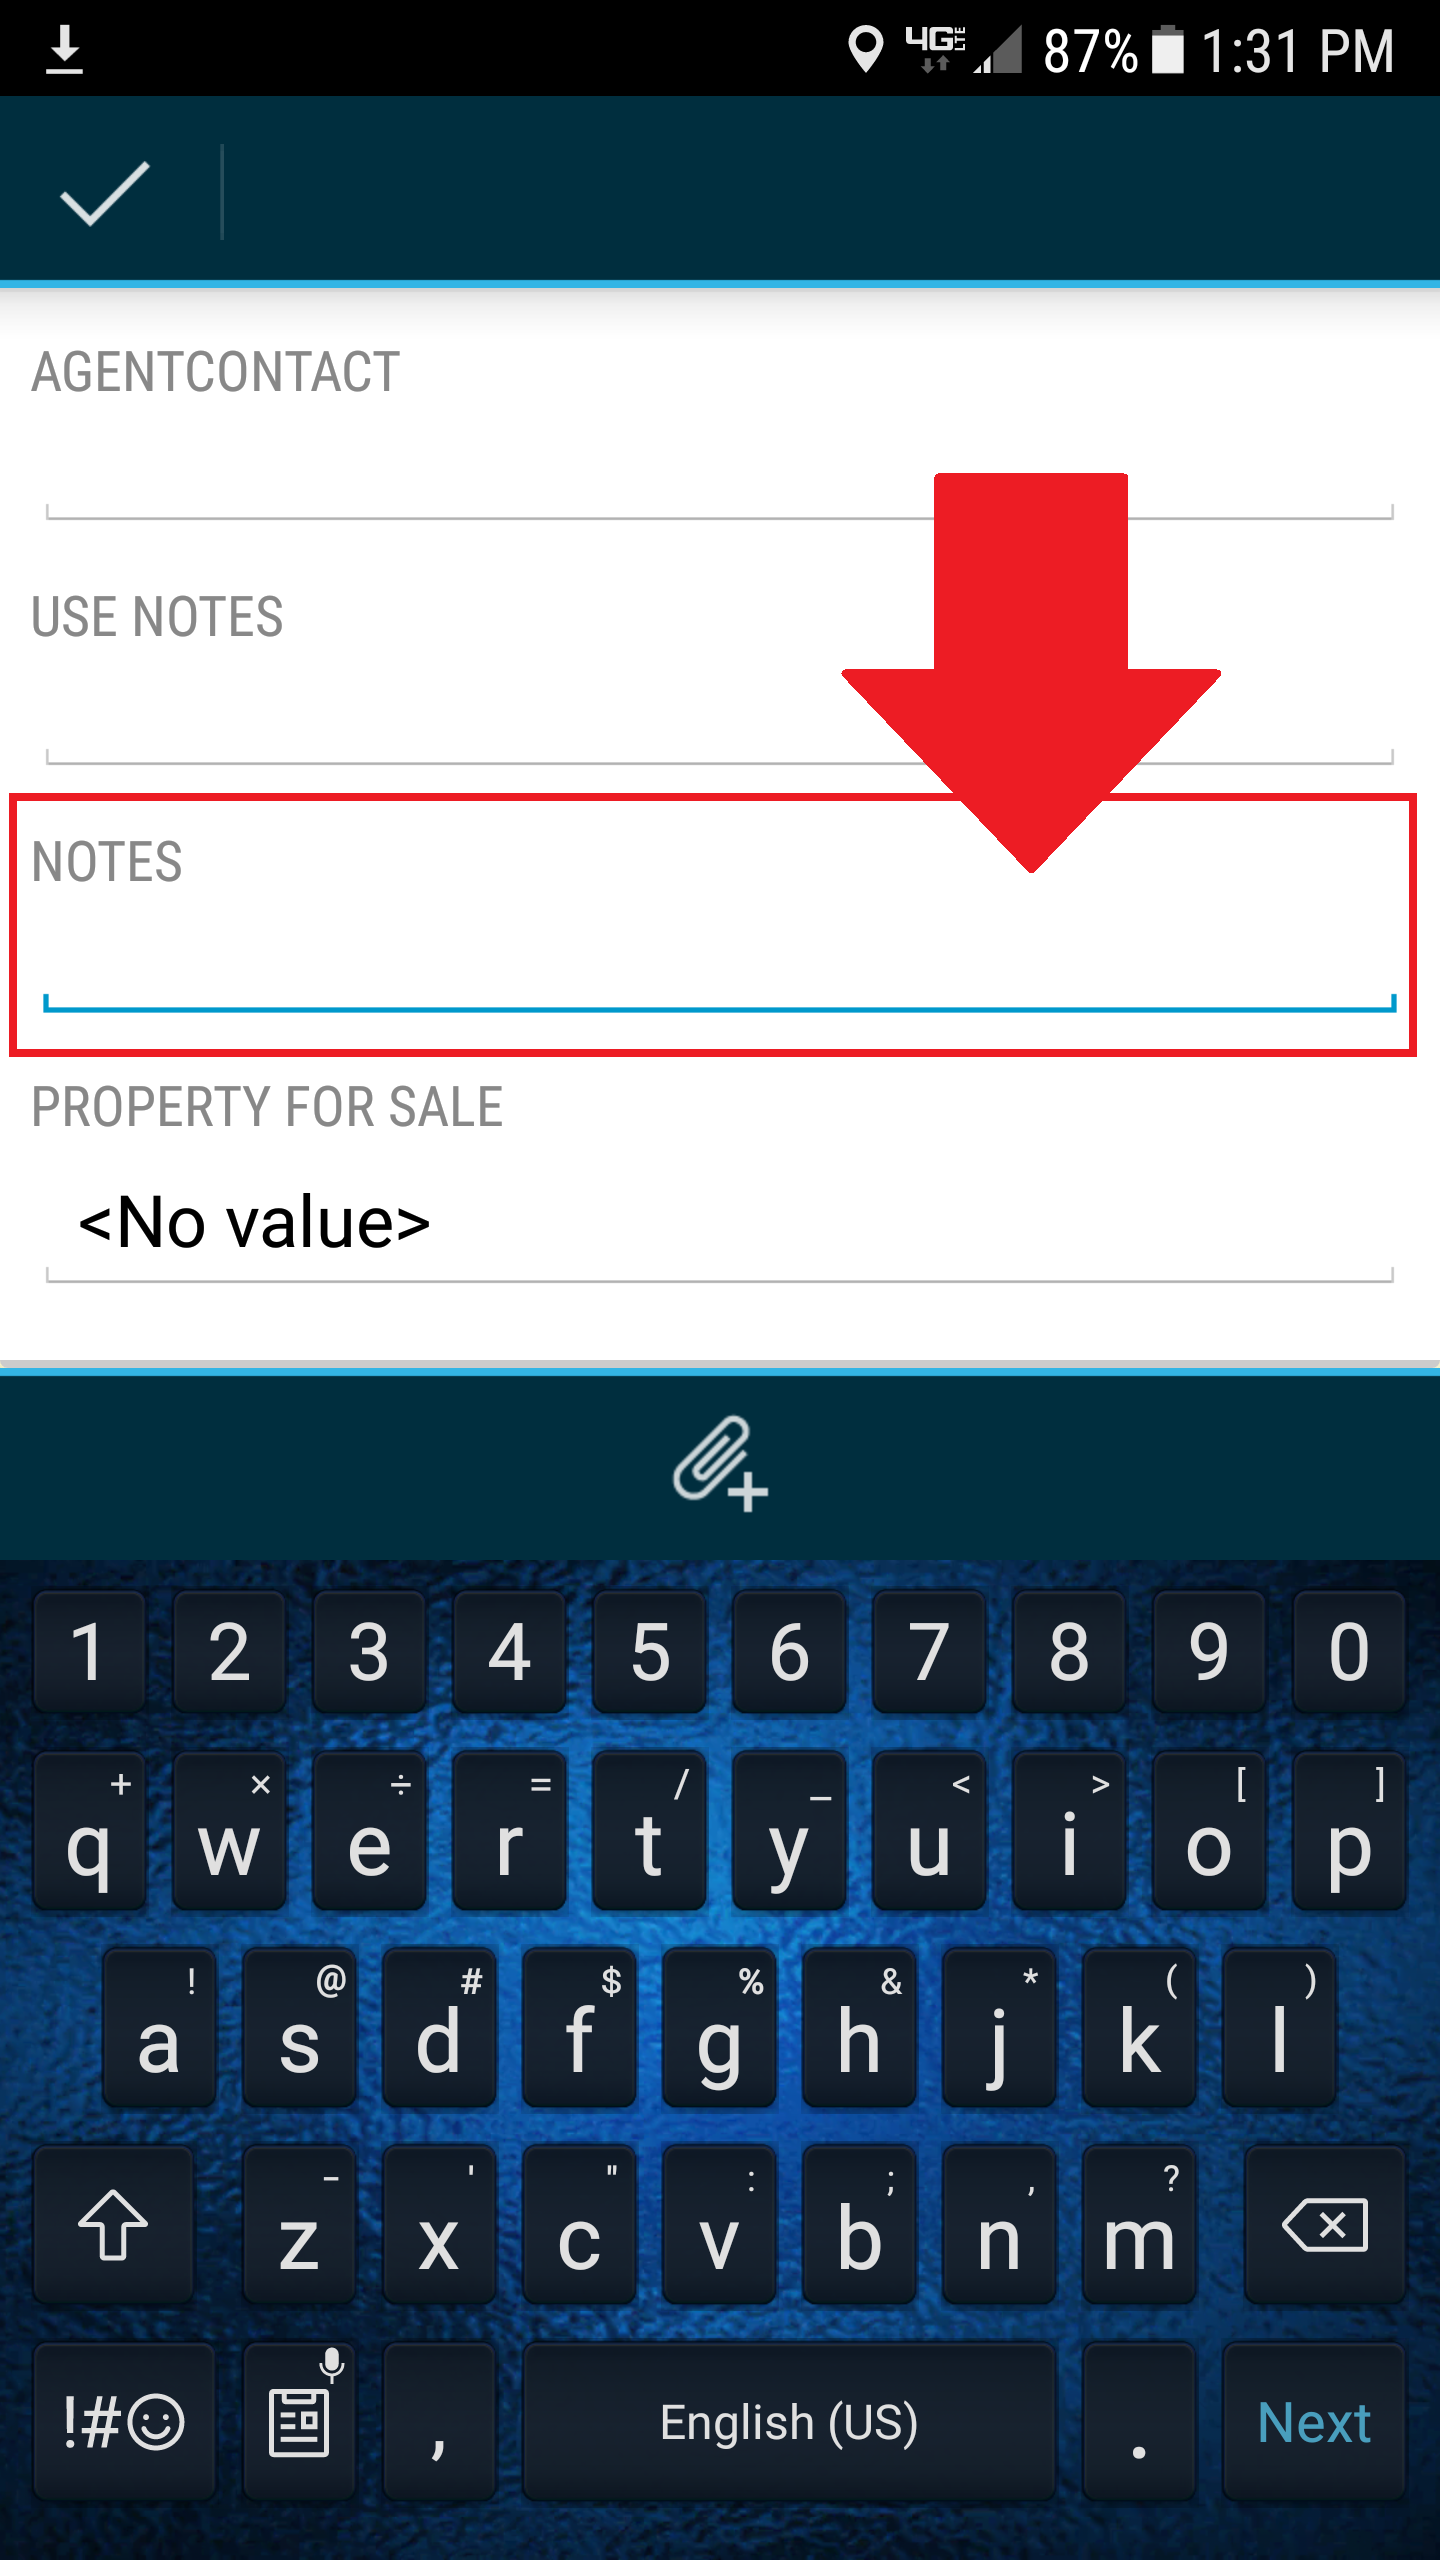
\includegraphics[width=.2\textwidth]{notes.png}
\caption{Property Contaminated}
\end{wrapfigure}
Enter notes up to 120 characters\\
\vspace{2in}

\noindent Adjacent Property Contaminated yes or no prefilled\\
\vspace{2in}

\noindent Enter Property Contaminated notes up to 120 characters\\

\clearpage
\subparagraph*{Device 1 Field Operation Cont.}
\subparagraph*{\\}
\begin{wrapfigure}{r}{0.5\textwidth}
\centering
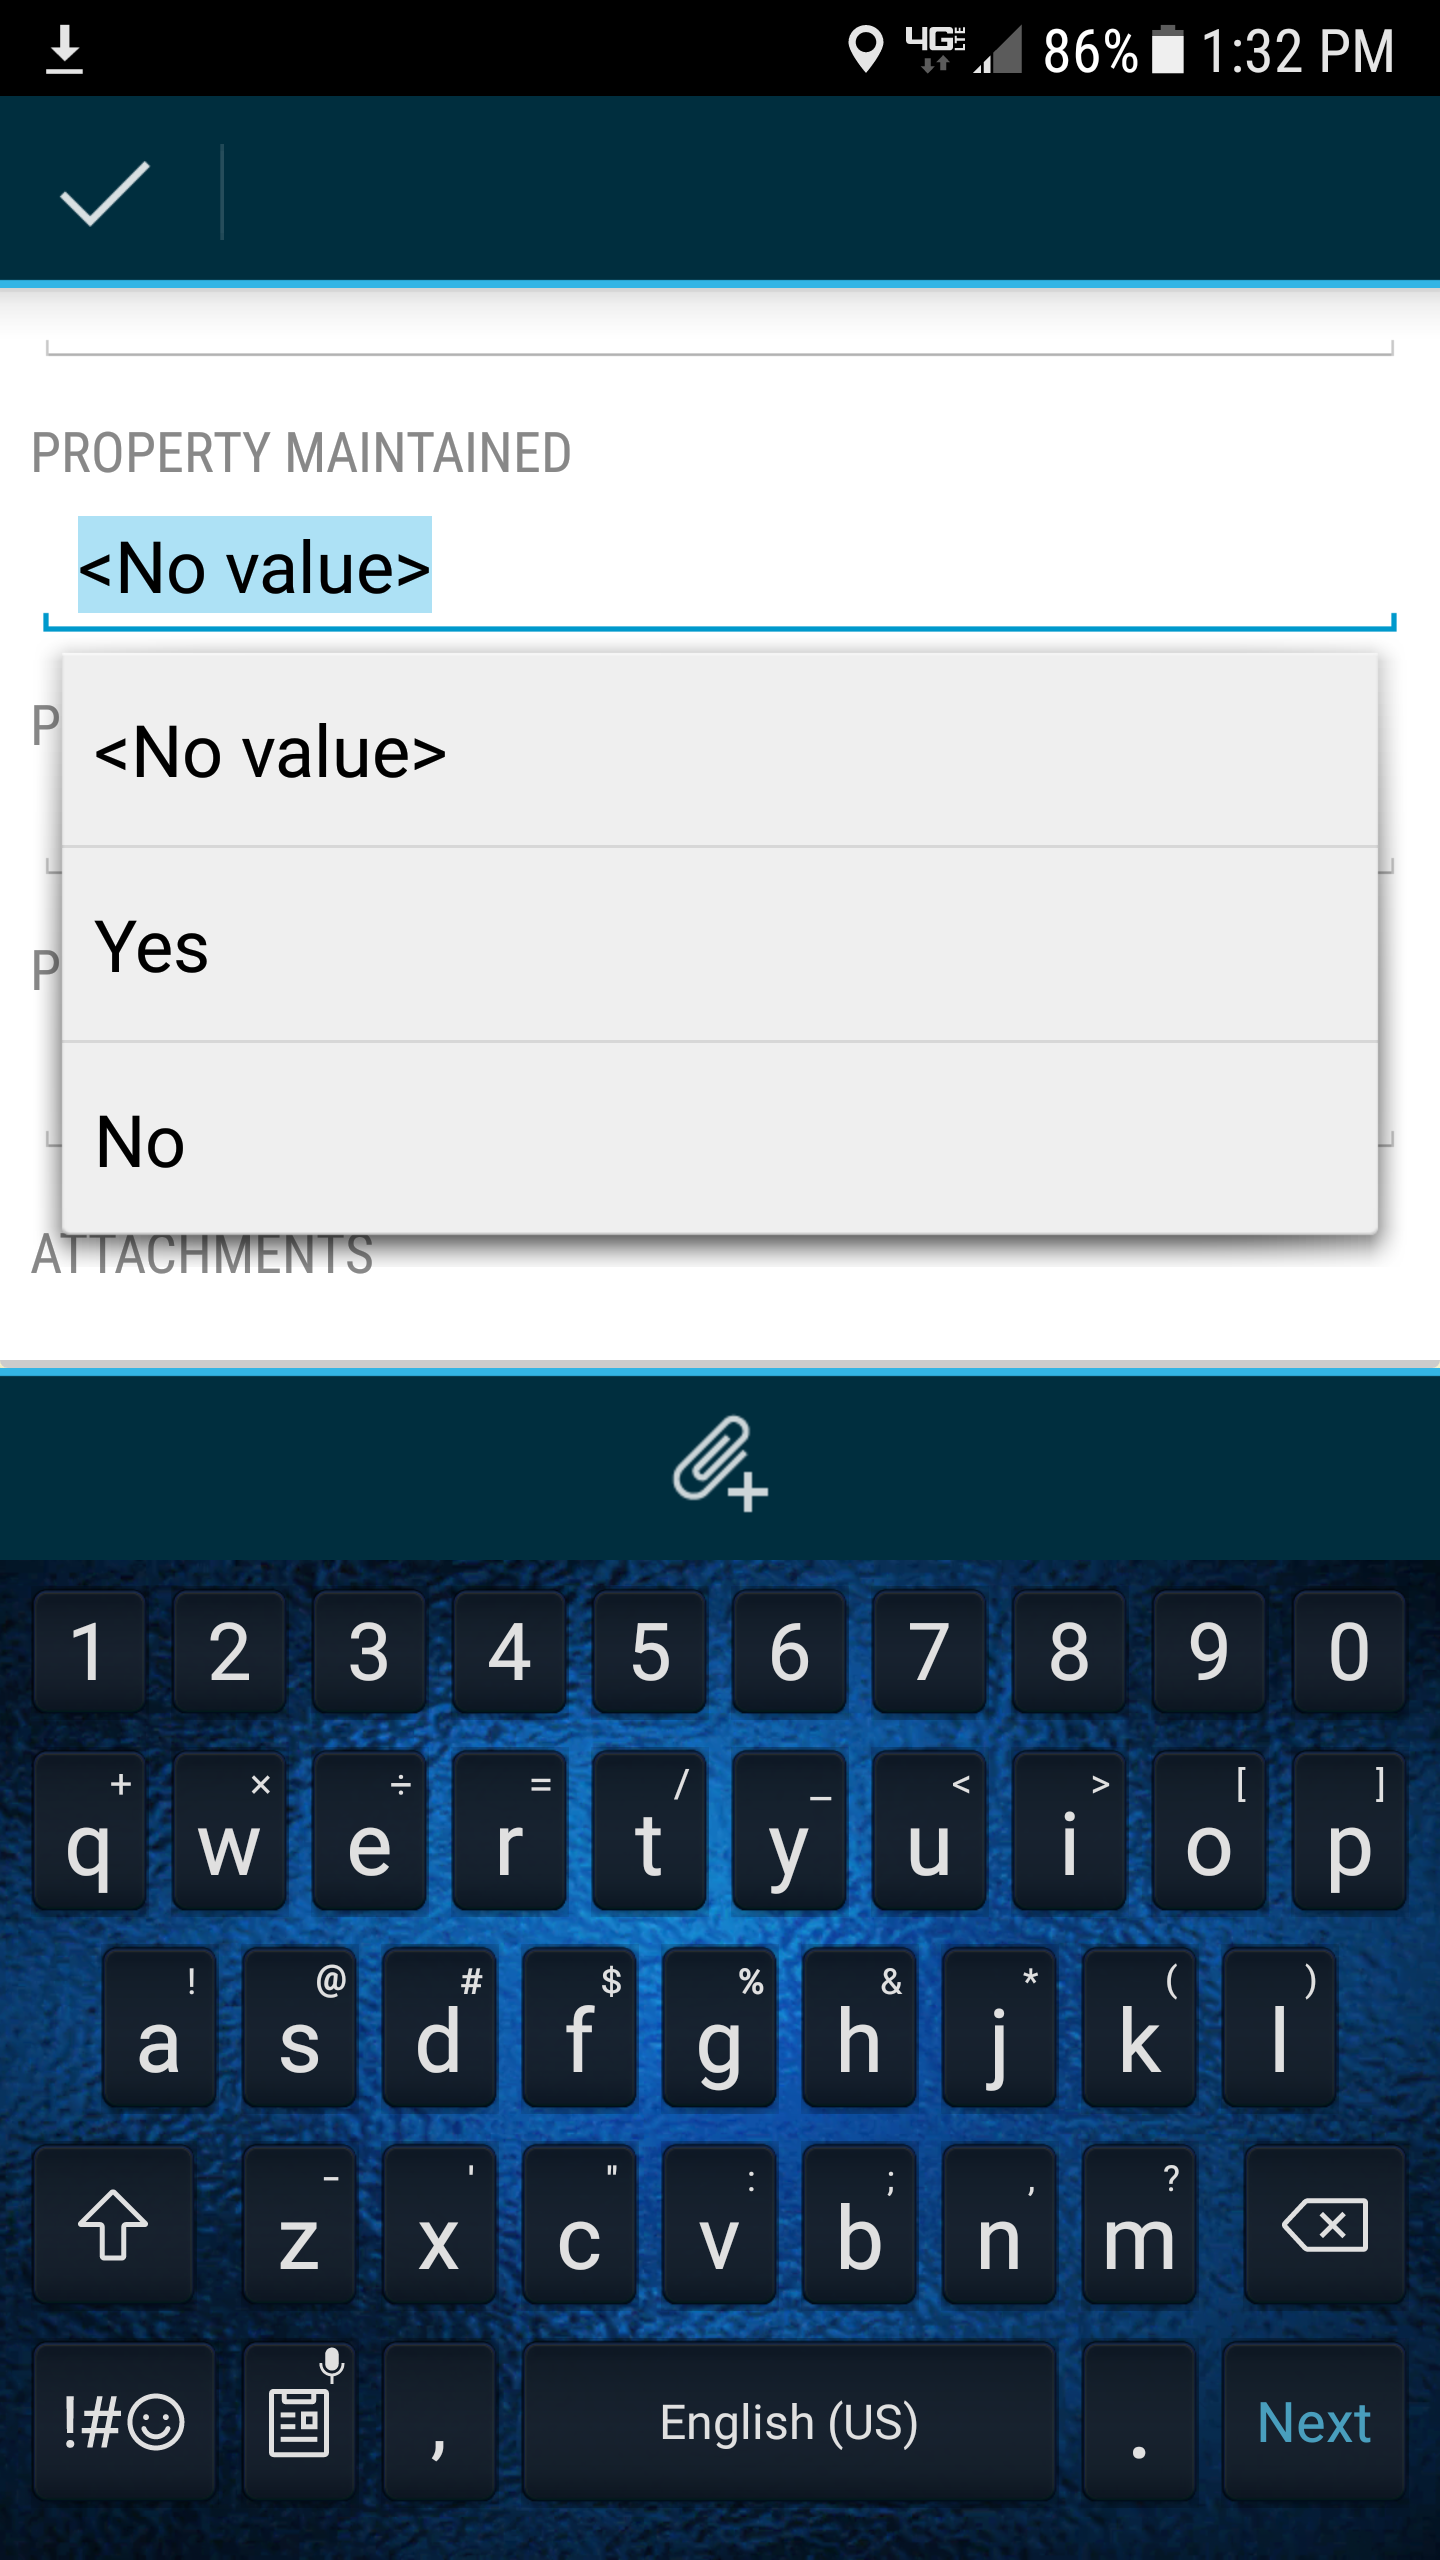
\includegraphics[width=.2\textwidth]{propertyMaintained.png}
\caption {Property Maintained}
\vspace{.15in}
\HRule \\[.4cm] % Horizontal Line added
\vspace{.2in}
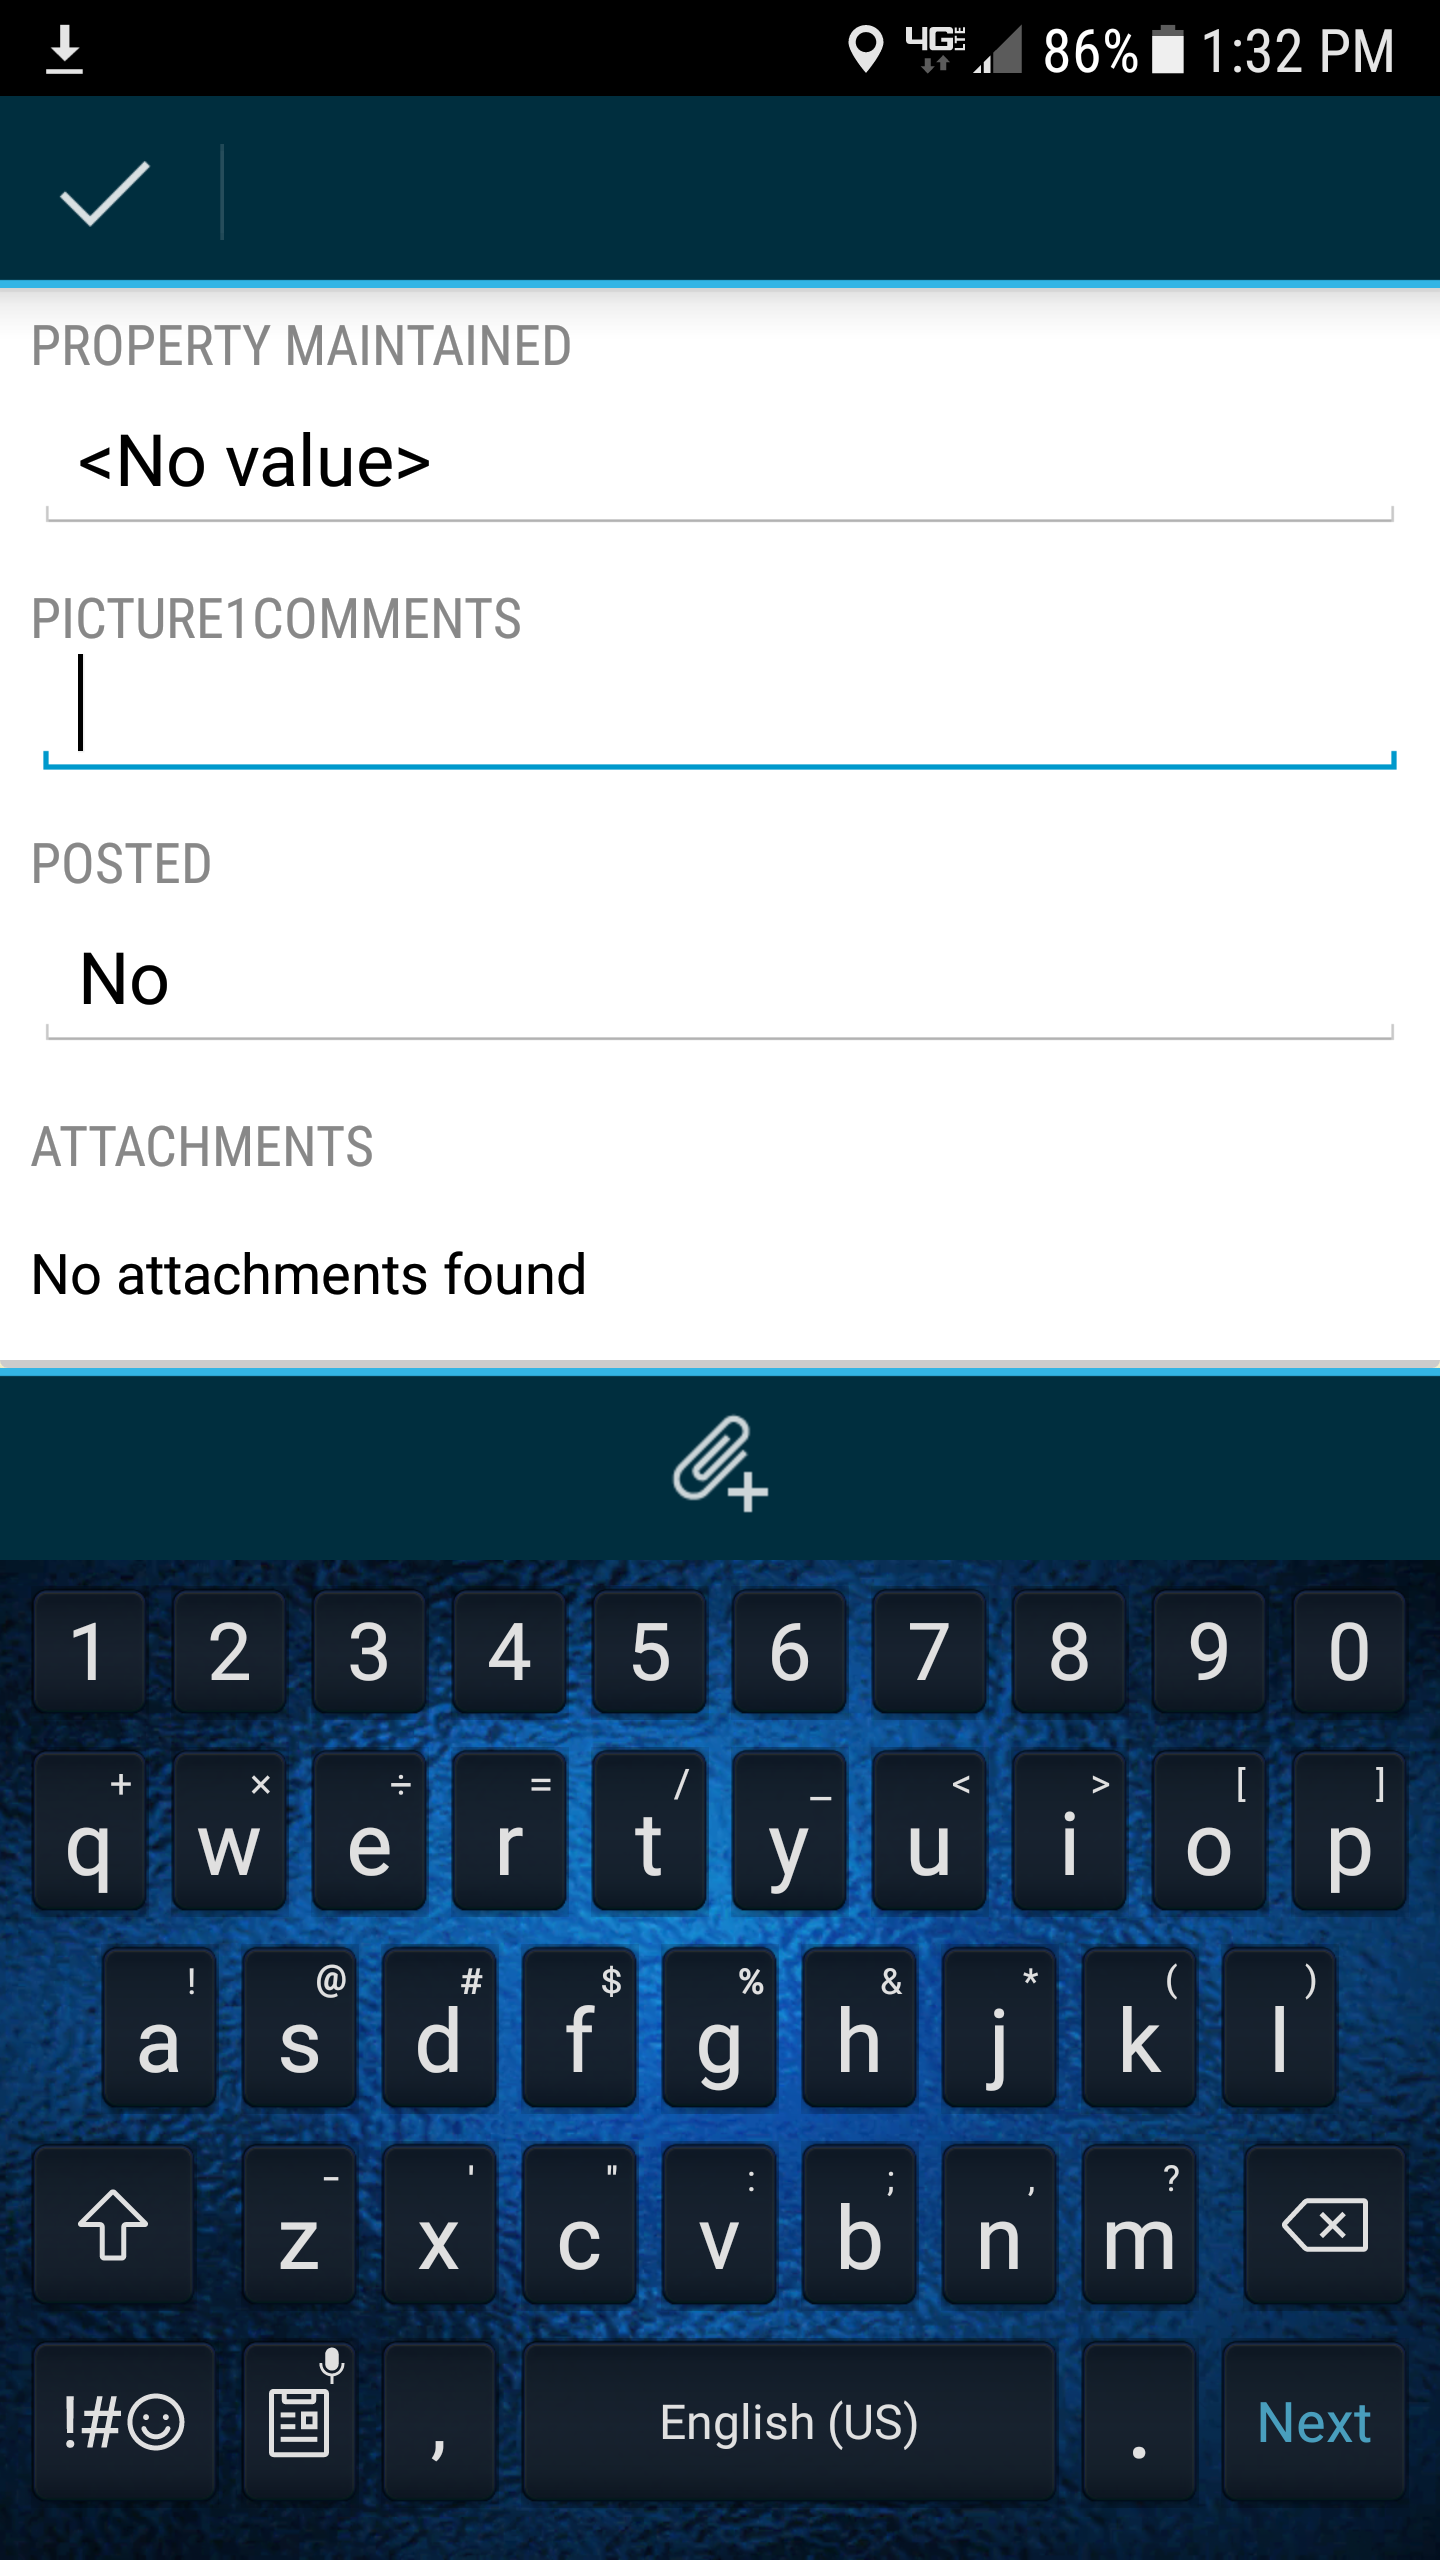
\includegraphics[width=.2\textwidth]{pictureComments.png}
\caption{Picture Comments}
\vspace{.15in}
\HRule \\[.4cm] % Horizontal Line added
\vspace{.2in}
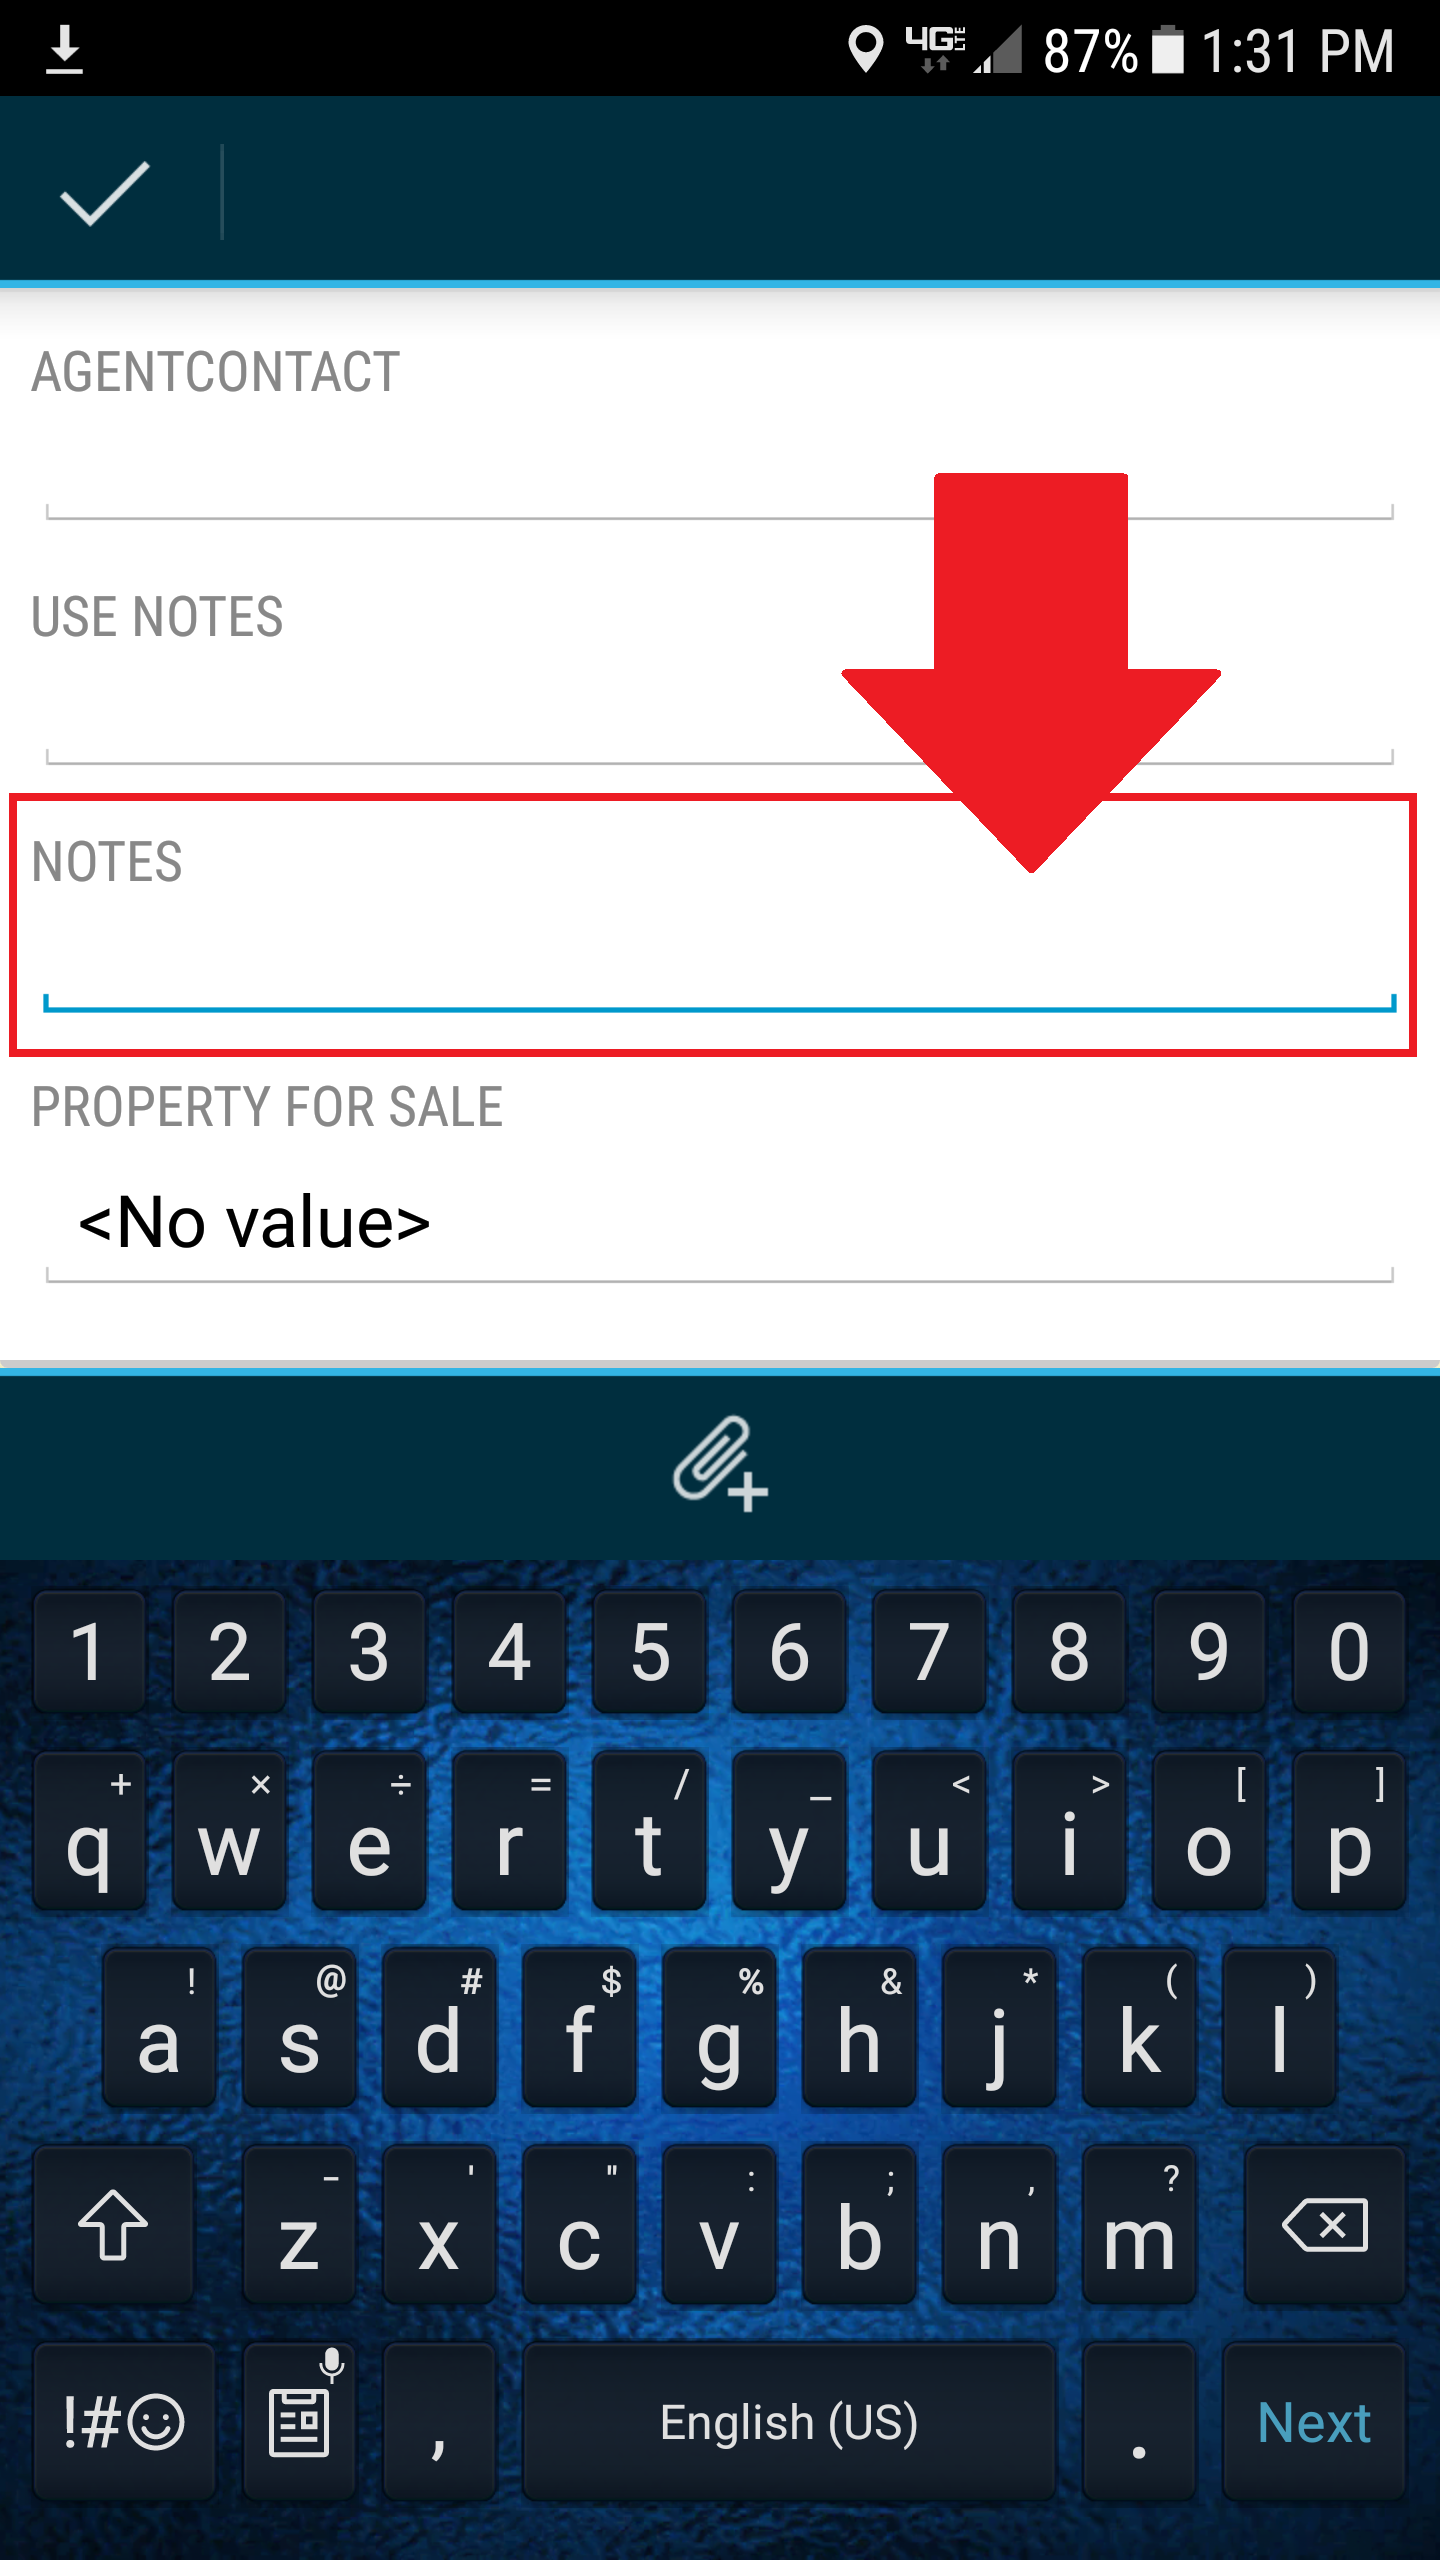
\includegraphics[width=.2\textwidth]{notes.png}
\caption{Placeholder}
\end{wrapfigure}
Property Maintained Yes or No\\
\vspace{2in}

\noindent Picture Comments up to 120 characters\\
\vspace{2in}

\noindent Placeholder\\

\clearpage
\subparagraph{Device 2 Field Operation}In the Forfeiture Field Map, for each site visited, a photo or photos can be added from the Open Camera Application.
%\subparagraph*{}In the Forfeiture Field Map, for each site visited, a photo or photos can be added from the Open Camera Application.

\begin{wrapfigure}{r}{0.5\textwidth}
\centering
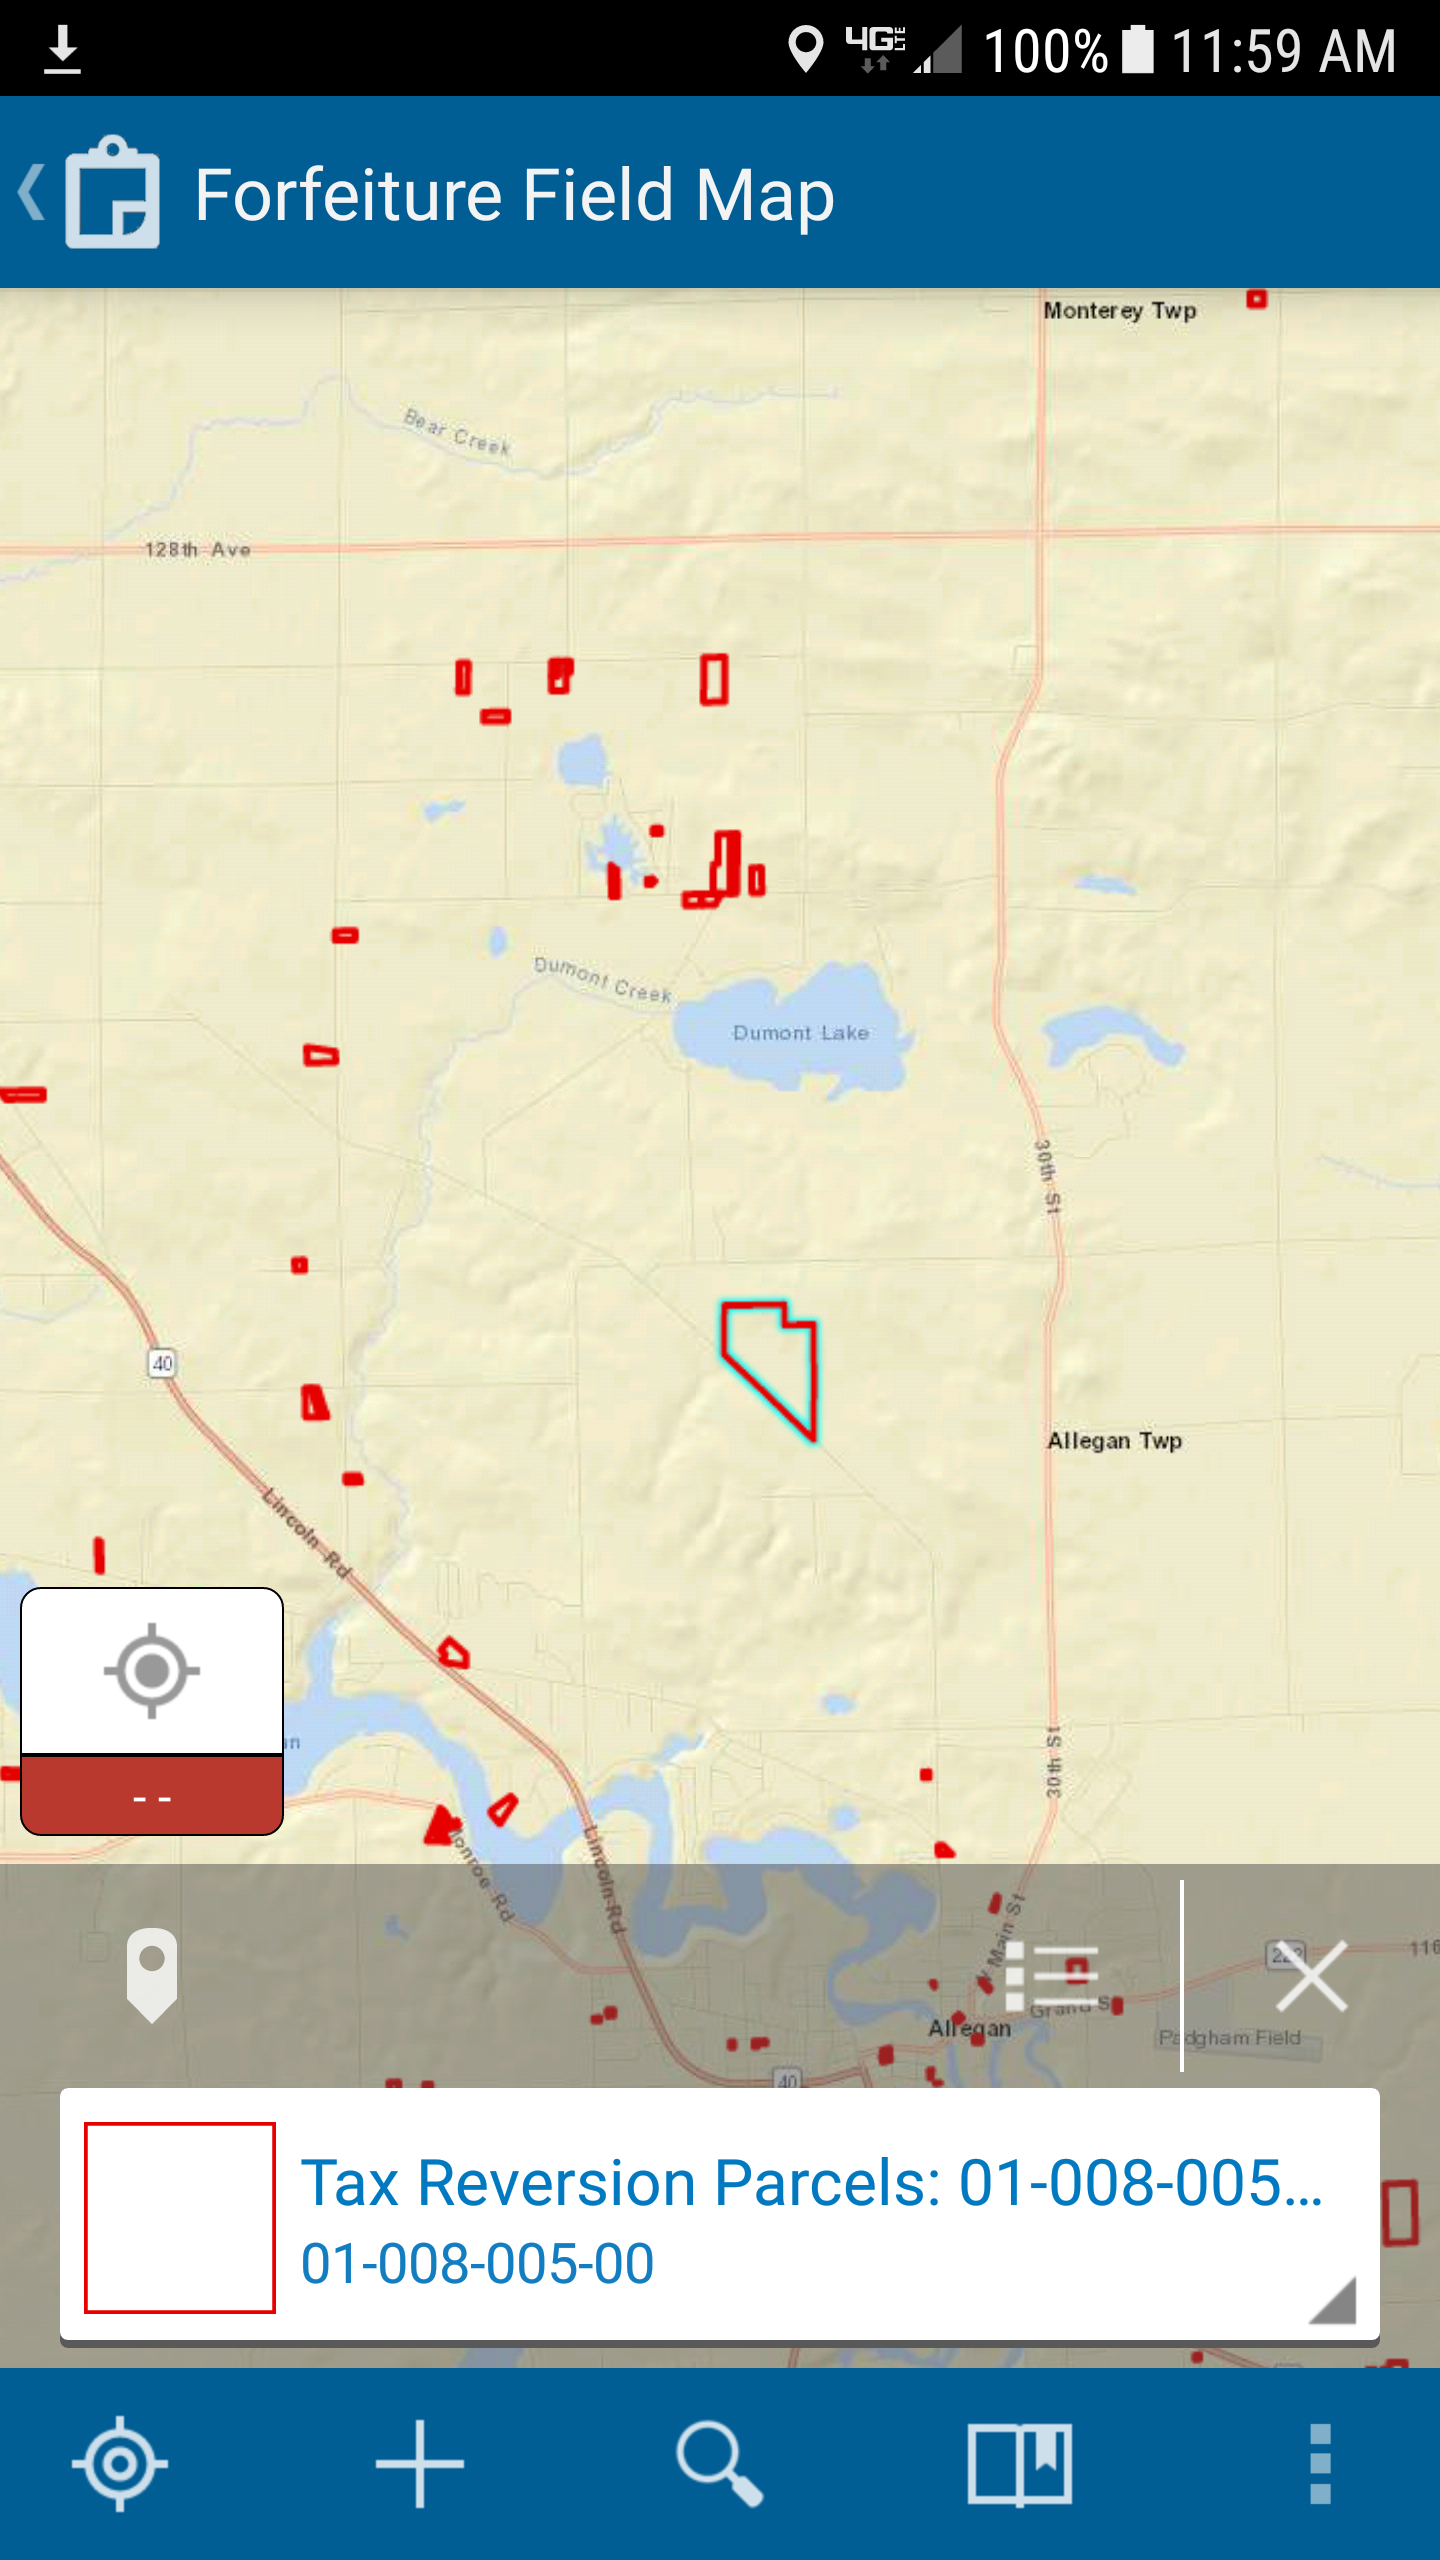
\includegraphics[width=.185\textwidth]{selectParcel.png}
\caption {Select Parcel}
\vspace{.15in}
\HRule \\[.4cm] % Horizontal Line added
\vspace{.15in}
\includegraphics[width=.185\textwidth]{pushAttachmentButton.png}
\caption{Push Attachment Button}
\vspace{.15in}
\HRule \\[.4cm] % Horizontal Line added
\vspace{.15in}
\includegraphics[width=.185\textwidth]{addAttachmentFromGallery.png}
\caption{Add Attachment From Gallery}
\end{wrapfigure}
\vspace{.5in}

Select a parcel from the map\\
\vspace{2in}

\noindent Push Attachment Button
\vspace{2in}

\noindent Select Gallery

\clearpage
\subparagraph*{Device 2 Field Operation Cont.} 
\subparagraph*{\\}

\begin{wrapfigure}{r}{0.5\textwidth}
\centering
\includegraphics[width=.2\textwidth]{openCameraFolderInGallery.png}
\caption {Open Camera Folder}
\vspace{.2in}
\HRule \\[.4cm] % Horizontal Line added
\vspace{.2in}
\includegraphics[width=.2\textwidth]{openCameraFolder.png}
\caption{In the Open Camera Folder}
\vspace{.2in}
\HRule \\[.4cm] % Horizontal Line added
\vspace{.2in}
\includegraphics[width=.2\textwidth]{imageInApp.png}
\caption{Image in the App}
\end{wrapfigure}
Navigate to the Open Camera Folder\\
\vspace{2in}

\noindent From within the Open Camera Folder, Select the appropriate image
\vspace{2in}

\noindent Press the check button to save the image to the parcel 

\clearpage
\paragraph{Daily Postprocessing Routine}Back at the office
\subparagraph{Synchronize Webmap}In Collector for ArcGIS, push the sync button on the Forfeiture Field Map
\subparagraph{Execute Postprocessing Script}A tool in ArcGIS that:

\begin{itemize}
\item Reconciles geodatabase versions
\item Generates forms for each site visited

%Insert screenshot of Postprocesing script in Arc here

\end{itemize}

\clearpage
\subsubsection{Software}
\paragraph{ESRI Licensed Products}
\subparagraph{ArcDesktop}Users of this application need a license to ArcGIS Standard level.

\subparagraph{Enterprise ArcGIS Deployment}This app uses ArcGIS Server and ArcGIS Portal.

\subparagraph{Collector for ArcGIS}Developed and tested on Android(7.0).  Collector is available at the Google Play Store.

\paragraph{Other Software}

\subparagraph{Open Camera for Android}

\begin{figure}[h!]
\centering
    \includegraphics[width=.7\textwidth]{openCameraAppStore.png}
\caption{Open Camera from Google Play Store}
\end{figure}

\end{document}